% The isotropic paper of Paper VII of the hemigroup programme (repository slug `affine`, module
% `iso`, tags iso-v0.1, ...; adr/0001): the isotropic theory in R^d, by reduction to the line, with
% the origin threshold d and the strict dimension filtration. Split on 2026-10-04 (Q-0307) from the
% single article in paper/, of which it was section 3 and Appendix A; the affine paper (paper/)
% restates the four statements of this one that it uses. Built on Paper V's model
% (spatial-hemigroup-scale-space, paper/ and paper-b/): one file per section, every statement shared
% with the blueprint under a `% shared with blueprint <label>` marker with the paper statement's own
% \label equal to the blueprint label (article-kit LINKAGE.md rule 4), so that `linkage check`
% reports it `verbatim`; the proofs of record from the blueprint, shortened where a proof is long;
% the cited facts stated as numbered theorems in section 2.6, each with the ledger's page anchor
% (blueprint/AXIOMS.md, never memory); section 1.1 owns the trust base (Table tab:trust-base,
% in Appendix B since Q-0428, says which statement rests on which cited fact), and the body
% carries no sentence of that kind before a statement
% (WRITING.md section 3; the dispatching session's decision of 2026-10-10, Q-0408, which reversed
% the earlier "printed in the prose before every [A] statement"); one relation-to-the-line
% remark; the frontier named where it occurs.
%
% Structure (adr/0001; notes/PLAN-article-structure.md). The file numbers are the single article's,
% so that section 3 here is blueprint chapter 3:
%   1  Introduction (Q-0307; 1.1 owns the trust base)
%   2  What is used from the line papers (no blueprint nodes; restatements by version; A1-A4)
%   3  The isotropic theory (blueprint ch. 3, parts/03-isotropic.tex)
%   4  Conclusion; 4.1 Open problems (the single article's problem on the origin in dimension d;
%      04-conclusion.tex, a conclusion since Q-0408, the author's review)
%   Appendix A: the proofs moved out of section 3 (Q-0291).
%   Appendix B: Verification, the inventory behind section 1.1 (Q-0414).
%   Back matter: the author's contribution and use of AI (ai-statement.tex) and the declarations
%   (declarations.tex), Q-0311. The declarations are final (Q-0313, the author's declarations of
%   2026-10-04) but for the release DOI; the AI statement is rewritten from the session archive by
%   the archivist (article-kit PROCESS.md § 8, pass 5).
%
% References into the released modules of Paper V cite them by their released statement numbers
% (repo CLAUDE.md): the line paper, \sscite{fagerstrom2026spatial}, tag v0.1, concept DOI
% 10.5281/zenodo.22761631; the cone paper, \sscite{fagerstrom2026cone}, tag cone-v0.1, concept DOI
% 10.5281/zenodo.22864169. No internal label reaches the reader (Q-0344, the author's review):
% shared text writes \prog{V}{Thm.~7.3} and \progpaper{B}, which macros.tex prints as citations,
% and the paper's own prose names the papers. Module C is not cited (the author, 2026-10-04). The affine paper of this
% repository and Paper VI are unreleased: prose about further work, never a \ref.
%
% Voice and register: article-kit docs/WRITING.md (neutral third person, the restraint budget).
% Build: cd paper-iso && latexmk -pdf main.tex. Gates before a commit: the build, `linkage check`
% with every shared statement verbatim, `linkage paper`. LaTeX is written with the file tools,
% never through shell heredocs.

% Q-0448 (the split into a paper and a supplement; records/affine/split_q0448.py and
% split_q0448_roots.py). Three roots, one set of sources:
%   main.tex        the paper (this file);
%   supplement.tex  the supplement: the trust base in full, the cited facts in full, the
%                   proofs that Lean checked, the inventory of the formal development;
%   full.tex        the one document: it defines \isofull and inputs this file, which then
%                   takes the four parts of the supplement as Appendices C to F.
% The paper and the supplement refer to each other through xr-hyper, so each is built after
% the other: python records/affine/build-paper-iso.py builds the three and checks them.
% The \date line below is the one `linkage release` reads; supplement.tex has a copy of it,
% and the build script fails when the two differ.
\documentclass[11pt]{article}
\ifdefined\isofull\else\newcommand{\isoexternal}{supplement}\fi
% Q-0448: the preamble of the three roots of the isotropic paper (main.tex, supplement.tex,
% full.tex), cut unchanged from main.tex by records/affine/split_q0448_roots.py, with the
% loading of xr-hyper added. The comments are those of main.tex.
\usepackage[a4paper,margin=1in]{geometry}
\setlength{\emergencystretch}{1.5em}
\usepackage{amsmath,amssymb,amsthm}
\usepackage{booktabs}
\usepackage{array}      % the ragged-right column R of Table tab:in-print
\newcolumntype{R}[1]{>{\raggedright\arraybackslash}p{#1}}
% Q-0430: Table tab:in-print is longer than a page since its cells carry the primary sources. It
% is a longtable, which breaks between rows; S is its column, R in the size of the table's text
% (the caption stays in the size of the other captions).
\usepackage{longtable}
\newcolumntype{S}[1]{>{\footnotesize\raggedright\arraybackslash}p{#1}}
% N: the column of Table tab:notation, a longtable too so that the two tables print in order.
\newcolumntype{N}[1]{>{\small}p{#1}}
\setlength{\LTcapwidth}{\textwidth}
% Q-0414, round 3: a float may fill most of a page with text below it. LaTeX's defaults send a
% table taller than 0.7 of the page to a page of its own, which Table tab:in-print would leave
% a quarter empty.
\renewcommand{\topfraction}{0.9}
\renewcommand{\textfraction}{0.08}
\renewcommand{\floatpagefraction}{0.85}
\usepackage{graphicx}   % the figure is a PNG from a script in records/ (*.pdf is git-ignored)
% Q-0448: the paper and the supplement refer to each other. A root that defines \isoexternal
% as the name of the other document gets its labels through xr-hyper, which has to be loaded
% before hyperref. The full document defines no \isoexternal. The option nocite keeps the other
% document's bibliography numbers out: each document has its own list of references, and
% without the option every citekey that both cite is reported as a label defined twice.
\ifdefined\isoexternal\usepackage{xr-hyper}\fi
\usepackage[hidelinks]{hyperref}
\ifdefined\isoexternal\externaldocument[][nocite]{\isoexternal}\fi
\hypersetup{
  pdftitle={Spatial Scale Space from Hemigroup Axioms: Rotation-Invariant Self-Decomposable Kernels in Dimension d},
  pdfauthor={Daniel Fagerstr\"om},
}

% Paper-side notation. Mirrors the notation half of blueprint/src/macros.tex (below its rule) so
% that statements shared verbatim with the blueprint compile here unchanged; Paper V's paper/ is
% the model (its macros.tex). Keep the two files in sync by hand: a drifted macro shows up as a
% compile error or a visibly different rendering, never silently. The notation is the programme's
% (hub RELEASES.md rule 3; ADR-0002 of the line repository), extended for d dimensions.
%
% \sscite is the blueprint's citation macro (framework-owned there); here it is plain \cite.

\newcommand{\sscite}[1]{\cite{#1}}

% -- Notation (mirrored from blueprint/src/macros.tex) -------------------------------------
\newcommand{\RR}{\mathbb{R}}
\newcommand{\CC}{\mathbb{C}}
\newcommand{\NN}{\mathbb{N}}
\newcommand{\ZZ}{\mathbb{Z}}
\newcommand{\Cin}{\operatorname{Cin}}   % the entire cosine integral, as in module B
\newcommand{\Levy}{L\'evy}              % the name, accented through one macro
\newcommand{\Matern}{Mat\'ern}          % the same device for the second member's name
\newcommand{\PD}{\mathrm{PD}}           % positive definite d x d matrices
\newcommand{\PSD}{\mathrm{PSD}}         % positive semidefinite d x d matrices
\newcommand{\GL}{\mathrm{GL}}
\newcommand{\Orth}{\mathrm{O}}          % the orthogonal group O(d)
\newcommand{\tp}{\mathsf{T}}            % transpose, written A^{\tp}
\newcommand{\tr}{\operatorname{tr}}
\newcommand{\rank}{\operatorname{rank}}
\newcommand{\diag}{\operatorname{diag}}
\newcommand{\Sym}{\mathrm{Sym}}         % real symmetric d x d matrices
\newcommand{\gl}{\mathfrak{gl}}         % all real d x d matrices, as a Lie algebra

% -- Paper-only convenience ----------------------------------------------------------------
% The blueprint's \ledger{A2} names a ledger entry. The comparison key of `linkage check`
% strips the macro with its argument on both sides, so the paper may render it as it likes; it
% prints the cited fact's name, as section 2.6 states them: C1-C4 for the ledger's A1-A4, C5 for
% A8 (Q-0316: the proofs of record are transcribed verbatim, \ledger included, so the macro maps the
% ledger name to the paper's). Q-0377: C6 for A10, Schoenberg's radial theorem, which section 1.1
% names as a cited fact the machine-checked Theorem thm:filtration-strict(3) rests on.
\makeatletter
\@namedef{ledgerC@A1}{C1}
\@namedef{ledgerC@A2}{C2}
\@namedef{ledgerC@A3}{C3}
\@namedef{ledgerC@A4}{C4}
\@namedef{ledgerC@A8}{C5}
\@namedef{ledgerC@A10}{C6}
% Q-0414: C7 for A11, Karamata's Tauberian theorem at the origin (Q-0416). Until this line the
% item of section 1.1 printed "cited fact A11".
\@namedef{ledgerC@A11}{C7}
\newcommand{\ledger}[1]{\@ifundefined{ledgerC@#1}{cited fact~#1}{\@nameuse{ledgerC@#1}}}
\makeatother

% The blueprint writes the programme's internal labels through two macros, \prog{V}{Thm.~7.3} and
% \progpaper{B}, and prints them as [V, Thm.~7.3] and [B] (blueprint/src/macros.tex). A reader of a
% paper is given the citation instead (Q-0344, the author's review of the isotropic paper: the
% labels mean nothing to a reader): V is the line paper, fagerstrom2026spatial (tag v0.1), B its
% cone module, fagerstrom2026cone (tag cone-v0.1). The comparison key of `linkage check` reads the
% macro source on both sides, so a shared statement stays verbatim. Robust, so that a statement's
% optional title may carry one (inside braces, as any \cite there).
\makeatletter
\@namedef{progkey@V}{fagerstrom2026spatial}
\@namedef{progkey@B}{fagerstrom2026cone}
\newcommand{\prog@key}[1]{\@ifundefined{progkey@#1}{\PackageError{macros}{No citation for the
  programme label #1}{}}{}\edef\prog@thekey{\csname progkey@#1\endcsname}}
\newcommand{\prog@cite}[2]{\cite[#2]{#1}}
\DeclareRobustCommand{\prog}[2]{\prog@key{#1}\expandafter\prog@cite\expandafter{\prog@thekey}{#2}}
\DeclareRobustCommand{\progpaper}[1]{\prog@key{#1}\expandafter\cite\expandafter{\prog@thekey}}
\makeatother

% \restated{V}{Def.~3.1}{def:line-family} and \restatedp (Q-0406, the author's review of the
% isotropic paper's section 3): a numbered place of the line paper or the cone paper that the
% isotropic paper restates in its section 2. The blueprint prints the located citation, as \prog
% does. A paper that carries the restatement under the label of the third argument sends its reader
% there ("Definition 2.1", "(2.1)", "section 2.3"), where the restatement carries the released number;
% a paper without that label prints the located citation. \restatedp is the same place cited as an
% aside, in parentheses. The kind word is read off the label's prefix. The two papers use this one
% definition; records/affine/check-restated-labels.py lists which uses resolve in which paper, and
% fails if one in the isotropic paper does not. The reference itself goes through \paperOrigRef,
% the copy of the kernel's reference command that the wrapper below takes at \begin{document},
% with the wrapper's rule for an equation label written out here. The reason is `linkage paper`:
% it reads a literal reference command whose argument is a macro parameter as a reference to a
% label of that name, and fails its lint on it. For the same reader the section sign is written
% \textsection: the one-letter command in a definition is reported as a bare section pointer.
\makeatletter
\newcommand{\restated@ref}[1]{%
  \IfBeginWith{#1}{eq:}{\textup{(\paperOrigRef{#1})}}{%
  \IfBeginWith{#1}{def:}{Definition~}{%
  \IfBeginWith{#1}{lem:}{Lemma~}{%
  \IfBeginWith{#1}{thm:}{Theorem~}{%
  \IfBeginWith{#1}{prop:}{Proposition~}{%
  \IfBeginWith{#1}{cor:}{Corollary~}{%
  \IfBeginWith{#1}{sec:}{\textsection}{}}}}}}\paperOrigRef{#1}}}
\DeclareRobustCommand{\restated}[3]{\@ifundefined{r@#3}{\prog{#1}{#2}}{\restated@ref{#3}}}
\DeclareRobustCommand{\restatedp}[3]{\@ifundefined{r@#3}{\prog{#1}{#2}}{%
  \IfBeginWith{#3}{eq:}{\restated@ref{#3}}{(\restated@ref{#3})}}}
% \restatedc: a clause, as (source clause)(restatement clause) in its last two arguments.
\DeclareRobustCommand{\restatedc}[5]{\@ifundefined{r@#3}{\prog{#1}{#2#4}}{\restated@ref{#3}#5}}
\makeatother

% Equations are cited with \ref in the blueprint (its render allowlist has no \eqref), and a
% statement shared verbatim must cite them the same way. So the paper wraps \ref, as Paper V's
% paper does: a label beginning `eq:` prints in parentheses, as \eqref would have; every other
% label is untouched. Installed at \begin{document}, after hyperref has finished redefining
% \ref. Use \ref for equations throughout the paper, never \eqref (double parentheses).
% The original is copied with \NewCommandCopy, not \let: the kernel's \ref is itself robust, so
% \let would copy only the wrapper and \DeclareRobustCommand would then loop (Paper V's lesson).
\usepackage{xstring}
\AtBeginDocument{%
  \NewCommandCopy{\paperOrigRef}{\ref}%
  \DeclareRobustCommand{\ref}[1]{\IfBeginWith{#1}{eq:}{\textup{(\paperOrigRef{#1})}}{\paperOrigRef{#1}}}%
}

\numberwithin{equation}{section}

\theoremstyle{plain}
\newtheorem{theorem}{Theorem}[section]
\newtheorem{proposition}[theorem]{Proposition}
\newtheorem{lemma}[theorem]{Lemma}
\newtheorem{corollary}[theorem]{Corollary}
\theoremstyle{definition}
\newtheorem{definition}[theorem]{Definition}
\newtheorem{example}[theorem]{Example}
\theoremstyle{remark}
\newtheorem{remark}[theorem]{Remark}

% \suppl names the place of what Lean checked, and \supplnumbers says how its numbers read.
\ifdefined\isofull
  \newcommand{\suppl}{the supplementary appendices}
  \newcommand{\supplnumbers}{The supplementary appendices are
    Appendices~\ref{supp:trust} to~\ref{supp:verification}.}
\else
  \newcommand{\suppl}{the supplement}
  \newcommand{\supplnumbers}{A statement, a section, an equation or a table whose number
    begins with an S is one of the supplement.}
\fi

\title{Spatial scale space from hemigroup axioms:\\
rotation-invariant self-decomposable kernels in dimension $d$}
\author{Daniel Fagerstr\"om}
% Q-0417: the build frozen for external review (article-kit PROCESS.md section 9) names its
% revision by the tag iso-review-1. "Not yet released" stays in the line, so that `linkage release`
% still reads it as a draft date. The working-draft line, for the first edit after the review
% rounds (a change after a freeze is a new freeze, with a new tag):
% \date{Working draft --- not yet released}
% Q-0432: the second freeze, after the response to the first external review.
% Q-0448: the third freeze, after the response to the second external round, the split into a
% paper and a supplement, and the Lean of the stages (Q-0447).
% The release iso-v0.1 (records/affine/freeze_iso_release.py): the date, the version and the
% version DOI, on one line, as in supplement.tex. The draft line, restored at the first edit
% after the release, is the working-draft line above.
\date{October 14, 2026 (v0.1)\\[3pt] {\normalsize \href{https://doi.org/10.5281/zenodo.23357468}{doi:10.5281/zenodo.23357468}}}

\begin{document}
\maketitle

% Q-0448: the abstract of the paper, cut unchanged from main.tex with the comments above it
% (records/affine/split_q0448_roots.py); main.tex inputs it, and with it full.tex.
% The abstract is new with the split (Q-0307), written for this paper alone: a probability paper on
% the isotropic theory, its four results by name. Each sentence was compared with the statement it
% restates (WRITING.md § 5): the classification with its sufficiency half
% (thm:isotropic-classification), the threshold for kernels with no Gaussian part and the Matern
% reading of its clause (3) (thm:origin-boundedness-d), the strict chain with A_infinity the
% subordinated slice ([B, Prop. 4.9], thm:filtration-strict, lem:threshold-limit), the Cin rays
% (thm:no-cin-ray-in-the-plane). Within 250 words.
% Q-0310 (the whole-paper review's fixes for this paper): "kernels from scale zero" throughout, so
% that "origin" means the centre of R^d only; the threshold sentence restricted to those kernels,
% as thm:origin-boundedness-d is, and the polar profile's normalization named (review flag 4); the
% strictness of Schoenberg's chain attributed to Gneiting (gneiting1999radial, p. 94), the
% self-decomposable chain kept as new (records/affine/PRIOR-ART-novelty-claims.md); the Cin
% sentence says A_2, which is what thm:no-cin-ray-in-the-plane proves.
% Q-0311 (the blind review records/affine/REVIEW-paper-iso.md): framed as a classification of
% kernel families (flag 8); the cascade named a hemigroup, the word of the title (flag 5); what is
% classical (the line threshold, the classification read on laws) said, and the three new results
% named as such (flags 1, 2); the Matern sentence says why the threshold is the Matern range: the
% kernel's density is the Matern function of smoothness gamma - d/2 (flag 9;
% READING-fischer2025variance.md); "the line's cone" defined before use (flag 32). Within 250 words.
% Q-0313 (the scope audit, records/affine/SCOPE-AUDIT-paper-iso.md): the Matern sentence says the
% density is a Matern function only for gamma > d/2, where the smoothness gamma - d/2 is positive (for
% gamma <= d/2 the same formula is no Matern function), and says "bounded" as clause (3) does; "in a
% suitable scale parametrization" dropped from the classification sentence, which holds in every
% gauge (mu_{0,t} is the dilation by chi(t) of the law with exponent F(|xi|)), to stay within 250.
% Q-0316 (pass 2, the blind register review REVIEW-register-paper-iso.md, section 4 flags 4, 5,
% 13, 14): five cited theorems (Wolfe's is C5); Wolfe's radially nonincreasing density in one
% sentence, not counted as new; the Matern sentence marked as a case of the threshold result, the
% kernel named (the variance-gamma law, Fischer et al.) and "a constant times"; "witnesses" and the
% second sense of "threshold" replaced. The title names the object (flag 10; the author's decision of
% 2026-10-05, following the proposal in records/affine/REVIEW-register-paper-iso-fixes.md). Within 250 words.
% Q-0328: the pointwise lower bound of prop:origin-lower-bound-d (d >= 2, c finite) in one sentence
% under the first result; to stay within 250, "of this programme", "convex", "released" and "of
% probability theory" dropped and "the classical semigroup in the scale" made "the one-parameter
% semigroup". 250 words (records/affine/check-paper-iso-backmatter.py).
% Q-0377 (the formalization closed, 125 of 125 nodes \leanok): the last sentence says the results
% are machine-checked and rest on six cited theorems (section 1.1; C6, Schoenberg's radial theorem,
% is new), as Paper V's abstract does in one clause; the line papers, which the formal proofs build
% on without resting on any cited fact of theirs, leave the sentence. To stay within 250, "By a
% theorem of Wolfe" became "By Wolfe's theorem". 249 words.
% Q-0381 (the fidelity review's paper-facing point 6): the profile is defined on (0, infinity), so
% "exceeds d at radius zero" and "a finite value c there" become "exceeds d near radius zero" (for
% a nonincreasing profile, the same as its limit at zero exceeding d) and "a finite limit c there".
% Word for word; still 249 words.
% Q-0414 (the repositioning pass, round 1; records/affine/REPOSITIONING-paper-iso.md): rewritten
% to lead with what section 1 and the conclusion lead with. The question (the axioms name no
% dimension: which families do they allow in R^d, and what does the dimension change); the
% answers in the reader's terms, with c as the power at which the transform falls off (Corollary
% cor:origin-profile-exponent(2)) and no class symbol; why they matter for a measurement (a point
% source recorded as a spike; a family of the line that gives none in the plane); what is new and
% what is not, after the prior art read for this item (the threshold classical on the line and
% assembled from known results in R^d; the radially nonincreasing density Watanabe's; the rate
% for d >= 2, the strictness from A_3 on and the Cin rays "new as far as the author has found");
% seven cited theorems, and "the statements of the main section" for what is machine-checked
% (section 1.1; the Matern sentence is an example drawn in prose). Each sentence compared with
% its statement: thm:isotropic-classification with lem:isotropic-realisation;
% thm:origin-boundedness-d(5) for a kernel from scale zero with no Gaussian part;
% prop:origin-rate-d; cor:origin-profile-exponent(3) ("in every dimension that admits the
% exponent"); thm:origin-boundedness-d(3) with prop:isotropic-bridge(2) for 1/2 < gamma <= 1;
% thm:filtration-strict; thm:no-cin-ray-in-the-plane with prop:line-extreme-rays.
% Q-0414, round 3 (the register review of 2026-10-11b, flags 3, 9, 10, 11, 21, 38, 39; the
% dispatching session's decision E): the family is named by its transform, with "Matern" as the
% gloss (the standard Matern kernel is bounded); the filtration sentence names its objects (the
% exponents allowed in dimension d + 1 are strictly fewer); no ordinals for the two ways the
% dimension enters; the threshold "not found stated for the class", its ingredients known; the
% subject first in the sentence on what is new.
% Q-0428 (the rewrite after the external review, round 1; the author's direction of 2026-10-12,
% records/affine/REVIEW-author-paper-iso.md, last section; records/affine/
% REPOSITIONING-paper-iso-round2.md). The order: the class of cascades and why the semigroup law
% is relaxed; the classification; the centre; the dimension; the verification. No sentence on
% what is new or was not found stated. "From scale zero" is said as "the kernels that take the
% signal to each scale" (the presentation review, item 5). The rate keeps its two forms apart:
% an asymptotic equivalence for c < d, a lower bound of logarithmic growth for c = d (the
% response record of batch R1, section 3; prop:origin-rate-profile-d(1) and (3)). Each sentence
% compared with its statement: thm:isotropic-classification with lem:isotropic-realisation;
% thm:origin-boundedness-d(5) for a kernel from scale zero with no Gaussian part;
% cor:origin-profile-exponent(3) ("can have": in every dimension that admits the exponent);
% thm:origin-boundedness-d(3) with prop:isotropic-bridge(2) for 1/2 < gamma <= 1;
% prop:origin-rate-profile-d(1): q(s) ~ Q s^(c-d) K(s), Q and K from the polar profile, K slowly
% varying (prop:isotropic-exponent-profile(1)); (3): q(s) ~ B L(s) with L(s) >= log(1/s);
% thm:filtration-strict(3); prop:radial-dictionary(2) and (3), said as "correspond to radial
% characteristic functions", without an article, because the abstract does not carry the two
% conditions on the law (no atom at the origin, a finite logarithmic moment);
% thm:filtration-strict(1) with lem:threshold-asymptotic(3). The last sentence is the trust base
% of section 1.1 in short: the dictionary with what is drawn from it and the closed form of the
% constant (lem:exponent-profile-constant) are not machine-checked; the description of the
% separating family as laws, which is not machine-checked either, is not in the abstract.
% 250 words (records/affine/check-paper-iso-backmatter.py).
% (The Lean of Q-0427, for the rate through the Levy measure and the limit of the critical
% values, is merged since.)
% Q-0428, the fixes round (the register review of the front, flags 2, 5, 6, 9, 14, 18, 19; the
% scope audit of 2026-10-12, rows 1, 8, 10, 14). What a hemigroup relaxes is said in the
% sentence that names it (two scale indices; a stage need not be one of the kernels that take
% the signal to a scale), with the axiom that makes the kernels dilations of one law. The word
% "exponent" is not used: the function is F, and "power" is kept for c. One function F of the
% radius gives the kernel on the line and in the plane. The rate is one clause; the constants,
% the two conditions of the dictionary and the asymptote of the critical values are in the body.
% Each sentence compared with its statement: thm:isotropic-classification with
% lem:isotropic-realisation; prop:isotropic-bridge(3) for the Gaussian and the stable kernels;
% thm:origin-boundedness-d(5) for a kernel from scale zero with no Gaussian part;
% prop:origin-rate-profile-d(1) and (3) (a constant in both regimes);
% cor:origin-profile-exponent(3) ("in each dimension that admits it, with the same c");
% thm:origin-boundedness-d(3) with prop:isotropic-bridge(2) for 1/2 < gamma <= 1;
% prop:profile-one-dimension-down(2) for "strictly fewer"; prop:radial-dictionary(2) and (3)
% ("determines a radial characteristic function": the direction from F to the law, which needs
% neither condition on the law to be stated); thm:separating-family-critical-values(4).
% The last sentence was then the second list of section 1.1 in words that matched its four
% items. Since Q-0448 it points to that list and names no count (below); the list has five.
% Word count: records/affine/check-paper-iso-backmatter.py.
% Q-0431 (the author's section review of 2026-10-12, records/affine/REVIEW-author-paper-iso.md).
% His three phrases ("and that name no dimension", "again", "The dimension enters twice") were
% in the abstract of the first review build and are not in this one, which Q-0428 rewrote. Read
% for the same defect, a phrase that points at something the abstract does not have: "one
% closed form" did not say of what, and is "a constant's closed form" (the closed form of the
% constant of the spike, lem:exponent-profile-constant; "with its constant" is five sentences
% up). The sentence "The kernels that take the signal to each scale are the dilations of one
% rotation-invariant self-decomposable law ... and every such law but the point mass occurs" is
% the main result of the contributions paragraph of section 1 and stands as it is, the first
% result after "This paper derives". 250 words.
% Q-0448 (the response to the second external round). Exposition item 1 of
% records/affine/reviews/VERIFY-round2-length-and-exposition.md: "self-decomposable" is glossed
% in a clause (Definition 15.1 of Sato, as section 1 has it: the law is the convolution of its
% image under x -> lambda x with another law, for every 0 < lambda < 1); "admits" is "allows",
% the word of the third sentence, and a sentence says that one F need not give a kernel in
% every dimension, which is prop:profile-one-dimension-down(2); the last sentence points to the
% list of section 1.1 and names no count, so that it stays true when a statement changes
% status. Item 9 of VERIFY-round2-mathematics.md (reviews A, R9, and D, R5): the F that
% determines a radial characteristic function is an allowed one (prop:radial-dictionary(2)
% starts from F in A_d). "As an explicit one-parameter family shows" is gone, for the words.
% Q-0448, the blind draft review after the split (records/affine/
% REVIEW-draft-paper-iso-q0448.md, flags 8, 9 and 10, with the dispositions beside it). Flag 8:
% e^{-F(t|xi|)} is the transform of the kernel at scale t in one labelling of the scales
% (thm:isotropic-classification has chi(t)), not of the one law, and F is introduced. Flag 9:
% "Gaussian part" is not used. The threshold is said for every kernel from scale zero, with
% c <= infinity the power at which the transform falls off: for a datum (a, k_d),
% -log mu-hat / log|xi| tends to k_d(0+) when a = 0 and to infinity when a > 0
% (cor:origin-profile-exponent(1) and (2)), and a kernel with a Gaussian part is bounded (the
% paragraph before thm:origin-boundedness-d), so "bounded exactly when c > d" holds for both,
% by clause (5) of the theorem for a = 0. In the body c is k_d(0+), which for a > 0 can be
% finite; the abstract's c is the power of the fall-off, and "finite c" there means a = 0 and
% k_d(0+) finite, the hypothesis of prop:isotropic-stages(2). The rate "and constant are
% given", with no Levy measure; "characteristic function" has its gloss, "the Fourier
% transform of a law"; the kernels have one name, the Matern kernels of section 1 on, and the
% Bessel scale space is named once. Flag 10: "One F need not give a kernel in every dimension"
% is gone, since "Each higher dimension allows strictly fewer F" says it, and the words go to
% the stages (prop:isotropic-stages(2), 0 < s < t). "c depends on F alone" is
% cor:origin-profile-exponent(2) and (3). Each
% sentence compared with its statement: cor:isotropic-scale-zero-kernels(1) and (3);
% thm:origin-boundedness-d(5); prop:origin-rate-profile-d(1) and (3) with
% lem:exponent-profile-constant(4); prop:isotropic-bridge(2) with
% thm:origin-boundedness-d(3); prop:profile-one-dimension-down(2); prop:radial-dictionary(2)
% and (3).
% Word count: records/affine/check-paper-iso-backmatter.py.
\begin{abstract}
Scale-space axioms usually require the cascade to be a semigroup, which with
rotation and scale invariance leads to Gaussian and stable kernels. The axioms studied here require
only that the stages compose, a hemigroup indexed by two scales, and that rescaling the signal relabels the scales. This paper derives the
rotation-invariant families they allow in $\RR^d$. The kernels that take the signal to each
scale are the dilations of one rotation-invariant law that is self-decomposable: the convolution
of each contracted copy of itself with another law. Every such law but the point mass occurs.
Suitably labelled, the kernel at scale $t$ has Fourier transform $e^{-F(t|\xi|)}$, for one
function $F$. Its density is bounded near the centre exactly when $c > d$, where
$c \le \infty$ is the power at which the transform falls off. Otherwise a point source
is recorded as a spike, whose growth and constant are given. For finite $c$ a
stage between positive scales passes a fixed fraction of the record unchanged. Since $c$
depends on $F$ alone, a kernel bounded on the
line can have a spike in the plane: the \Matern{} kernels of the Bessel scale space,
with transform $(1 + |\xi|^2/2)^{-\gamma}$, do for
$\tfrac12 < \gamma \le 1$. Each higher
dimension allows strictly fewer $F$. An allowed $F(r) \sim c\log r$ determines a radial
characteristic function, the Fourier transform of a law, and is allowed in $\RR^{d+1}$
exactly when that function is a characteristic function there. The statements are
machine-checked in
Lean~4, assuming seven theorems of the literature, except those that \S\ref{sec:trust-base}
lists as proved in print.
\end{abstract}


% §1 Introduction of the isotropic paper --- new with the split (Q-0307, 2026-10-04; adr/0001),
% assembled from the single article's introduction (paper/01-introduction.tex before the split): its
% second paragraph on the axioms of the line papers, its paragraph "The isotropic corner reduces to
% the line" with the comparison with Schoenberg, its contribution 2, its scope sentence on the line
% theory, and the part of 1.1 that concerns section 3, each moved with the wording the new context
% needs. New: the question of this paper alone, the Matern reading of the threshold (from section
% 3.3), the plan. Every sentence that restates a result was compared with its statement
% (WRITING.md § 5). Nothing here is shared with the blueprint.
%
% 1.1 owns the trust base (article-kit PROCESS.md § 7, WRITING.md § 4): the state of the
% formalization, the four cited facts with the statements that rest on them (the blueprint's
% ledger, blueprint/AXIOMS.md, and the cited-fact sentences of section 3), and the figure.
%
% Q-0310 (the whole-paper review's fixes for this paper; records/affine/
% REVIEW-paper-whole-fixes-paper-iso.md): the strictness of Schoenberg's chain is Gneiting's (1999,
% p. 94, Euclid's hat; READING-gneiting1999radial.md, PRIOR-ART-novelty-claims.md).
%
% Q-0311 (the blind review records/affine/REVIEW-paper-iso.md; its flags answered in
% REVIEW-paper-iso-fixes.md): "hemigroup" defined in the first paragraph, with Hazod-Siebert as
% Paper V cites it (Def. 2.14.16, p. 380; READING-hazod2001stable.md) (flag 5); the comparison with
% the classical axioms stated once, as Paper V states it, against Pauwels et al. (flag 12); the
% kernels from scale zero, never "from the origin" (flag 24); the question framed as a
% classification of kernel families (flag 8); a paragraph on prior work in probability (Sato
% Thm. 16.1, p. 99, by Sato 1991, p. 117; Hazod-Siebert Thm. 2.14.21, p. 383; Sato Thm. 28.4 and
% Lemma 28.5, p. 191, by Zolotarev and Wolfe, Rem. 28.6, p. 193; READING-sato1999levy-prior-art.md)
% and one on the scale-space neighbours (Pauwels et al. p. 695; Duits et al. pp. 267, 277) (flags
% 1, 2, 17); the novelty paragraph and the contributions narrowed to the three new results, and its
% two self-contradictions removed (Schoenberg's Theorem 6 is on the infinitely divisible class, as
% the intersection; the witness family is [B]'s) (flags 6, 7, 10, 22); the reduction sentence kept
% here and in 3.2 only (flag 33); the trust base in plain words, with the cited facts renamed C1-C4
% (flags 3, 25, 28).

%
% Q-0316 (pass 2, the blind register review records/affine/REVIEW-register-paper-iso.md; every flag
% answered in REVIEW-register-paper-iso-fixes.md): the prior-work paragraphs split into short
% sentences and a list (flags 6, 7); (ND) named and the parametrization hedge dropped (flags 9, 10);
% the Matern kernels said to have Matern densities, for gamma > d/2, with no third nu (flags 11,
% 13); Sato's two-sided k named as his (flag 12); the line's cone, the folded profile, the
% subordinated slice and the Cin rays pointed to section 2 where they are first used (flag 1); the
% bridge's hypothesis named (flag 2); the frame and the new results made to agree (flag 3); the
% scale-space neighbours positioned against the isotropy axioms of Koenderink, Florack et al.,
% Florack and Lindeberg, each read at the page (flag 15; READING-koenderink1984structure.md,
% READING-florack1992scale.md, READING-florack1997image.md, READING-lindeberg2011generalized.md);
% Wolfe's theorem as the cited fact C5 and the radially nonincreasing density as a proposition; the
% trust base lists every import and says what the line papers' own trust bases are (flags 4, 14).
%
% Q-0328: prop:origin-lower-bound-d (Q-0272, refereed blind) in "The answer", in contribution 1 (the
% same topic, so still three results) and in 1.1 (it spends C3(iii) only, ledger A3(iii); no new
% cited fact). Each sentence compared with the statement: d >= 2, c finite, almost everywhere.
%
% Q-0344 (pass 6, the author's review of this section; every comment answered in
% records/affine/REVIEW-author-paper-iso.md): rewritten as questions, then answers, in plain
% language. No internal label: the earlier papers are named as a reader would ("the line paper",
% "the cone paper", each with its citation; a numbered place in them is \prog{V}{...} or
% \prog{B}{...}, printed as a located citation, macros.tex). Self-decomposable laws cited where they
% are defined (Sato Def. 15.1, p. 90, and Thm. 15.3, p. 91; Steutel-van Harn Ch. V, (1.1), whose
% stored copy prints no page numbers; READING-steutel2004infinite.md), and the Matern covariance
% (Matern 1960, (2.4.5)-(2.4.7), pp. 17-18; Stein 1999, pp. 31 and 48-49; Guttorp-Gneiting; Porcu et
% al.; READING-matern1960spatial.md, READING-stein1999interpolation.md). The reduction to the line
% explained by the projection of a rotation-invariant vector; the bridge explained as a Brownian
% motion run for a random time, citing the time-causal paper (fagerstrom2026hemigroup, Thm. 7.3) and
% the cone paper's Lem. 4.2 and Prop. 4.5. Zolotarev and Wolfe cited from their own papers, read at
% the page (READING-zolotarev1963structure.md, READING-wolfe1971continuity.md). The three prior-work
% paragraphs open with the question they position the paper against; the detail moved to its
% section: the line threshold with Sato's constant to 2.4 (it was there already), the polar
% criterion's attribution to 3.2, Schoenberg's Theorem 6 to 3.4. Every sentence restating a result
% compared with its statement (WRITING.md section 5).
%
% Q-0377 (the formalization closed: 125 of 125 blueprint nodes \leanok, main at dfafe99): 1.1 is
% rewritten as "What is machine-checked" on Paper V's model, with the cited fact C6 (Schoenberg's
% radial theorem, ledger A10), the headline #print axioms block and the trust-base markers
% `linkage check` reads; the contributions end with one clause on the formalization, and the plan
% counts six cited facts. The fidelity review (Q-0376) is named as pending in 1.1.
%
% Q-0407 (the author's decision on pull request #100): the classification on operators is a
% statement, Corollary cor:isotropic-classification-operators (section 3.2), machine-checked. "The
% answers" and "Scope" name it; 1.1 lists it under "What is proved", in the table's row for
% C3(ii), to which the row for C3(iii) refers, and in the #print axioms block. The abstract is
% unchanged: its sentence "classifies the rotation-invariant kernel families" is the theorem, and
% it is at 249 words.
%
% Q-0408 (pass 6, the author's review of sections 3.3, 3.4 and 4): checked against the new
% openings of 3.3 and 3.4 and the conclusion, so that the three tell one story. Two edits. In "The
% answers", c is introduced first as the power at which the kernel's transform falls off, the
% reading 3.3 opens with (Lemma lem:isotropic-exponent-log(1) with clause (1) of the theorem give
% log mu-hat / log|xi| -> -c), and then as the limit of the polar profile; "the density of its
% small jumps measured on the scale of |x|^{-d}" is gone ("jumps" was never introduced; section 2
% says "displacements"). The plan names section 4 as the conclusion with the open problems (4.1).
% The third answer already asks the question of 3.4 in its terms ("an exponent of the line, read
% as a function of |xi|"), and the abstract is unchanged.
% Second round (the blind register review of the new prose, REVIEW-register-paper-iso-q0408-fixes.md):
% "every such law ... occurs" cites Lemma lem:isotropic-realisation with the theorem, as section
% 3.4 and the conclusion do; "Scope" says what Remark rem:isotropic-line now holds (the comparison
% at d = 1) and that the not-carried list is section 4.1's.
% The same round removed from sections 3.3 and 3.4 every sentence that said which cited facts a
% statement "rests on" (the dispatching session's decision of 2026-10-10: WRITING.md section 3
% gives that to this subsection). Each was first compared with Table tab:trust-base, and 1.1
% gained what the sentences said and the table did not: C3(ii) is read by clause (1) of
% Proposition prop:isotropic-radial-monotone only and clause (2) reads C3(iii) with C2 (as
% the Lean has radial_monotone_family and radial_monotone_law), and the lower
% bound is verified for every law whose transform is the datum's, C3(iii) entering through the
% law of a truncated datum (origin_lower_bound takes a law mu with IsLawOf D mu).

%
% Q-0414 (the repositioning pass, round 1; records/affine/REPOSITIONING-paper-iso.md has every
% claim of novelty or attribution made here with the statement that carries it, the source, its
% anchor and the reading note). The section is rewritten against the prior art read after the
% paper was written (records/affine/PRIOR-ART-origin-threshold-reading.md): the questions carry
% their stakes for a measurement; "transform", "exponent", "Gaussian part" and "Levy measure" are
% said at first use; the second answer is in frequency-side words (c is the power at which the
% transform falls off, Corollary cor:origin-profile-exponent(2)); the dimension enters twice,
% through the class A_d and through the threshold d; one name for the Matern kernels, introduced
% once with their identification as the symmetric variance-gamma laws; the prior work on the
% centre of the kernel (the line: Zolotarev, Wolfe, Sato for continuity, Sato-Yamazato for
% boundedness and for the rate, Hartman-Wintner; R^d: Watanabe, Knopova-Schilling,
% Bogdan-Grzywny-Ryznar, Grzywny-Ryznar-Trojan, Cho-Kang-Kim); the cone paper positioned in the
% paragraph on the dimension filtration (cone paper, Prop. 4.9, Lem. 4.12(3), Rem. 4.10 and
% Figure 4, read at the page images of pp. 34, 38 and 39 for this item); the contributions as
% the queue item states them. 1.1 keeps the statement of the trust base; its inventory is
% Appendix B (appendix-verification.tex).
% Anchors: grzywny2019asymptotic by statement number of the published text (advance-access
% pagination 1-66; the journal pages 7193-7258 are not verified). (cho2021estimates and
% bogdan2014density, named above, are no longer cited: the rewrite of Q-0428 removed them.)
% Q-0424 (records/affine/reviews/VERIFY-round1-claims-and-trust-base.md, item 9): the paper
% cites grzywny2019asymptotic by statement number only and never by page, so nothing waits on its
% journal folios. One number collides with the first arXiv version, Corollary 5.8 (there Theorem
% 5.8 is another statement and the corollary is absent; READING-grzywny2019asymptotic.md,
% section 7), and Table tab:in-print says "of the published article" at that citation.
%
% Q-0424 (batch R1 of the response to the external review of round 1; records/affine/reviews/
% RESPONSE-round1-R1.md has every finding with what was done). In this file: question 2 says
% what an unbounded kernel does to the record of a point source, in the invariant form (no
% version of the density bounded near the centre), where it said "no finite value to sample"; and
% section 1.1 (its opening, the departures of C5 and C6, the paragraph on C5, the caption of
% Table tab:trust-base, the closed form of A_beta under "Outside the formal verification"). The abstract, "The
% answers", the prior-work paragraphs and the contributions are not touched: they are the
% framing batch's (R4), written once after the new statements are in.
%
% Q-0428 (the rewrite after the external review, round 1; records/affine/
% REPOSITIONING-paper-iso-round2.md has every attribution made here with its anchor and note, and
% every sentence on what the paper contributes with the statement that carries it). The author's
% direction of 2026-10-12 (records/affine/REVIEW-author-paper-iso.md, last section): the paper is
% a paper in scale-space theory; no apparatus of novelty; attribution exact and made once. So:
% the opening says why the semigroup axiom is relaxed and what that admits (the presentation
% review, item 1); mu_{0,t} and "from scale zero" are defined at first use, with "centre" for the
% point x = 0 (item 5); the answers carry the eight statements of Q-0425 (the rate through the
% polar profile, the dictionary and its consequences, the limit of the critical values) and say
% each result once; the Cin rays are introduced as elementary exponents, with the sentence on
% their superpositions and Jurek and Vervaat's Theorem 7.2 (item 14;
% READING-jurek1983integral-driving-process.md); the bridge is a Gaussian variance mixture before
% it is a process (item 15); "Scope" stands with the answers and names what is not treated (item
% 2). The three paragraphs "Prior work" and the list of contributions in two tiers are replaced
% by "Relation to scale-space theory", "Relation to probability" and "What the paper
% contributes". The anchors of the probability literature are in Table tab:in-print, once.
% 1.1, as first written in this item: two lists, machine-checked and not, with three statements
% written as machine-checked ahead of the Lean of the parallel item Q-0427. That Lean is merged
% since, and the fixes round (below) rewrote the subsection.
% cygan2017asymptotic and leonenko2013tauberian are cited in the numbering of their arXiv
% versions and bingham1997abel in that of the Hokkaido preprint: these are the copies held and
% the ones the paper cites (the author, 2026-10-12), said once, in the caption of Table
% tab:in-print. Their published numbering was not compared.
%
% Q-0428, the fixes round (records/affine/REPOSITIONING-paper-iso-round2-fixes.md has every flag
% of the register review of the front and every row of the scope audit of 2026-10-12 with what
% was done). The order of section 1: the cascade, what the semigroup axiom adds and what
% dropping it gives up and gains; the paper's question, with the axioms on kernels in one
% sentence, on the first page; what is known on the line, with the definitions the answers need;
% what the weaker axiom admits; the questions; the answers, each opening with its claim and held
% to the level of the questions (the two forms of the rate with their constants, the formula
% and the conditions of the dictionary, the sentence on the Urbanik representation and the limit
% of the critical values are in the leads of sections 3.3 and 3.4 and in the sources); scope;
% the two relations; the contributions as three items with their sections; the plan.
% Each sentence on the scale-space literature is held to its reading note (the scope audit,
% section 5): scale invariance is named with rotation invariance; Koenderink's route is a
% diffusion equation, not a semigroup; "stable" is this paper's word for the kernels of Pauwels
% et al. and of Florack et al.; Florack et al. are cited for the words of p. 380, whose formulas
% the note did not read on the page image; Florack's book with its p. 57 for "positive Schwartz
% filters". No sentence places the Matern kernels in the scale-space literature: no reading note
% supports one (the register review's flag 12 is a lead for the librarian).
% Section 1.1: three opening sentences (what Lean checked, what it did not, who compared the
% formal statements with the printed ones), the two lists with each print-only statement named
% in words, what is assumed, then the caveats, short, with the accounts statement by statement
% in Appendix B. The second list had four statements when the Lean of Q-0429 was merged, and
% has five since Q-0448 (Proposition prop:step-exponent-dimensions).

\section{Introduction}\label{sec:introduction}


% Q-0448 (the response to the second external round; records/affine/reviews/
% VERIFY-round2-scale-space-literature.md, sections 2, 3 and 10.2). With rotation and scale
% invariance the semigroup axioms leave the transforms e^{-t|xi|^p}, and positivity leaves
% 0 < p <= 2, the Gaussian included; a further requirement singles the Gaussian out (the order
% was the other way round). The two-scale cascade has its precedent, the causality axiom of
% Alvarez, Guichard, Lions and Morel (p. 203, at the page image; READING-alvarez1993axioms-
% architecture.md). "What is given up with the semigroup is an evolution equation" is gone:
% they obtain one without a semigroup, from locality, which is what is not asked here.
% Q-0448, the blind draft review after the split (records/affine/
% REVIEW-draft-paper-iso-q0448.md, with its dispositions beside it), group 2: one telling in
% section 1. The cascade and the aperture are defined in the first paragraph (flag 19); "stable"
% has its range where the kernels are first written (flag 13; Sato's Theorem 14.14 is for
% 0 < alpha <= 2, the Gaussian included, and so is clause (3) of Proposition
% prop:isotropic-bridge); the first paragraph points to "Relation to scale-space theory" for
% the causality axiom of Alvarez et al. and for what singles the Gaussian out, each of which is
% said there, once (flags 11, 12); that no generator is claimed is a limitation, in section 4
% (flag 7). The second paragraph states the axioms and leaves the questions to their list
% (flag 20).
A scale-space representation measures a signal through an aperture whose size is the scale. A
measurement is convolution with a probability kernel, and the record at a coarser scale is
computed from the record at a finer one by a further convolution, a \emph{stage}. The stages
together are the \emph{cascade}, and the \emph{aperture} at scale $t$ is the kernel that takes
the signal itself to its record at scale $t$.
Scale-space axioms usually require the cascade to be a semigroup in one scale parameter, as those of
the extended class of Pauwels, Van Gool, Fiddelaers and Moons do \sscite{pauwels1995extended}. A
semigroup requires more than a cascade needs: every stage has to be itself one of the apertures, so
that one parameter indexes the stages and the apertures alike. With rotation and scale
invariance the semigroup axioms of the literature leave the probability kernels whose Fourier
transform at the frequency $\xi \in \RR^d$ is $e^{-t|\xi|^p}$, for one $p$ with $0 < p \le 2$.
This paper calls them the \emph{stable kernels} of index $p$. The Gaussian is the stable kernel
of index $2$. The axioms studied here require only that the stages compose. With
$\mu_{s,t}$ the kernel of the stage from scale $s$ to scale $t$, this is
$\mu_{r,t} = \mu_{s,t} * \mu_{r,s}$ for $r \le s \le t$, and how a stage depends on its two
scales is left free. Such a family is a \emph{convolution hemigroup}
(\sscite{hazod2001stable}, Def.~2.14.16, p.~380). What is gained is a larger class of
apertures. The two-scale cascade has a precedent in scale-space theory, and ``Relation to
scale-space theory'' below sets the present axioms beside it and beside the semigroup axioms.

The axioms are those of the author's paper on the line \sscite{fagerstrom2026spatial}, the
\emph{line paper} below, with rotation invariance in place of the reflection symmetry
(Definition~\ref{def:isotropic-operator-family}): an aperture has a size, and no shape and no
preferred direction. Read on the kernels, they say that the stages
compose, that they depend continuously on the pair of scales, that each is rotation invariant,
and that a dilation of the signal only relabels the scales
(Definition~\ref{def:isotropic-kernel-family}). A family of kernels with these properties is an
\emph{isotropic cascade family}, an \emph{isotropic family} for short. The axioms read the same
in every dimension. In imaging $d$ is $2$ or $3$.

On the line the families are classified in the line paper
(Theorem~\ref{thm:line-classification}), and a second paper \sscite{fagerstrom2026cone}, the
\emph{cone paper}, describes the set of them. What is used from the two is restated in
\S\ref{sec:line}. A kernel is a probability measure, and that classification, like everything
after it in this paper, rests on the theory of such measures in probability. So from here on
the paper uses the vocabulary of that theory: a kernel is a \emph{law}, and its Fourier
transform, the transfer function of the smoothing, is the characteristic function of the law.
Stage, scale and cascade keep their meaning, and ``kernel'' stays in use for a law in its role
as an aperture. A frequency is written $\omega$ on the line and $\xi$ in $\RR^d$, and
$\widehat\mu(\omega) = \int e^{i\omega x}\,\mu(dx)$ is the Fourier transform of a kernel $\mu$
on the line, its \emph{transform} for short. The axiom on dilations
makes the apertures, the kernels $\mu_{0,t}$ \emph{from scale zero}, the dilations of one law:
up to a relabelling of the scales, $\mu_{0,t}$ has the
transform $e^{-F(t|\omega|)}$ for one function $F$, the \emph{exponent} of the family. The
cascade makes that law \emph{self-decomposable}: for every $0 < \lambda < 1$ it is the
convolution of its own image under $x \mapsto \lambda x$ with another law
(\sscite{sato1999levy}, Def.~15.1, p.~90; \sscite{steutel2004infinite}, Ch.~V, (1.1)). In a
cascade this is the relation between two scales. The kernel at the finer scale is a contracted
copy of the kernel at the coarser one, and the other law is the stage between them. Every
symmetric self-decomposable law other than the point mass occurs. Such a law is the convolution
of a centred Gaussian, which may be absent, with the law of a sum of independent displacements.
A law of the second kind alone has \emph{no Gaussian part}. Its \emph{\Levy{} measure} gives the
expected number of displacements of each size. On the line the density of that measure at the
size $x$, the two directions counted together and multiplied by $x$, is the \emph{folded
profile} of the law. In $\RR^d$ the same quantity is
taken in polar coordinates, the \emph{polar profile} of \S\ref{sec:isotropic-reduction}. The
Gaussian part and the profile determine the exponent, and the exponent determines them
(\S\ref{sec:line-axioms}; Proposition~\ref{prop:isotropic-polar-reading}(1)).

% Q-0448, the blind draft review (flags 12 and 13): what the semigroup axioms arrive at is said
% in the first paragraph and, with its sources, under "Relation to scale-space theory"; here
% the stable kernels are named as laws. The Bessel scale space is described there, once.
This is what the weaker axiom admits. In probability the stable kernels are the
rotation-invariant stable laws (\sscite{sato1999levy}, Thm.~14.14, p.~86). Among the kernels
added are the laws on the line with transform
$(1 + \omega^2/2)^{-\gamma}$, $\gamma > 0$, whose folded profile is $2\gamma e^{-\sqrt2\,x}$.
This paper calls these laws and their dilations the \emph{\Matern{} kernels} of index $\gamma$.
Scale-space theory knows them as the kernels of the Bessel scale space (``Relation to
scale-space theory'' below). On the line the kernels of integer index are those computed by a
cascade of identical first-order recursive filters, run forward and backward along the signal
(\prog{B}{Prop.~7.2 and Cor.~5.5}). Read as functions of the length $|\xi|$ of a frequency
$\xi \in \RR^d$, the transforms of the stable and the \Matern{} laws are the
transforms of self-decomposable laws on $\RR^d$, for every $d$
(Propositions~\ref{prop:line-filtration}(2) and~\ref{prop:isotropic-bridge}). For
$\gamma > d/2$ the density of the \Matern{} kernel on $\RR^d$ is a \Matern{} covariance
function, of smoothness $\gamma - d/2$. Spatial statistics uses that family to model random
fields whose smoothness is a parameter, and \Matern{} obtained it as a gamma mixture of
Gaussians (\sscite{matern1960spatial}, (2.4.5)--(2.4.7), pp.~17--18;
\sscite{stein1999interpolation}, \S2.7, p.~31, and \S2.10, pp.~48--49;
\sscite{guttorp2006studies}; \sscite{porcu2024matern}). In probability the \Matern{} kernels are
the symmetric variance-gamma laws \sscite{fischer2025variance}, and in potential theory their
densities are dilations of the Bessel kernel \sscite{aronszajn1961theory}
(Example~\ref{ex:matern} has the formulas).

\paragraph{The questions.} Three questions arise.
\begin{enumerate}
\item Which kernel families do the axioms allow in $\RR^d$? Their kernels from scale zero are
the apertures that a scale space with these axioms can use in the plane and in space.
\item What does the dimension change in a kernel? Chiefly, is the kernel bounded at its
\emph{centre}, the point $x = 0$, or does it record an ideal point source as a spike?
\item Does the exponent of a family of the line, read as a function of $|\xi|$, give a family in
the plane and in space? This is the rotation-invariant extension of the family, not the
separable one. The Gaussian and the $\alpha$-scale spaces of Duits et al.\
\sscite{duits2004axioms} pass. Is that general,
or does the set of allowed exponents shrink as $d$ grows?
\end{enumerate}

% Q-0448 (the author's decision of 2026-10-13: what is said twice goes; exposition item 4 of
% records/affine/reviews/VERIFY-round2-length-and-exposition.md): "The answers" and "What the
% paper contributes" are one passage. It opens with the main result, as the author's section
% review of 2026-10-12 asked of the contributions, and the two descriptions follow as the second
% and the third answer.
\paragraph{The answers.} The main result answers the first question. A probability law on
$\RR^d$ is a kernel from scale zero to a positive scale of an isotropic family, an aperture of a
scale space with these axioms, exactly when it is
rotation invariant, self-decomposable and not the point mass at the origin. In every isotropic
family the kernels from scale zero are, up to a relabelling of the scales, the dilations of one
such law, and every such law gives an isotropic family, for every relabelling of the scales
(Corollary~\ref{cor:isotropic-scale-zero-kernels}, with
Theorem~\ref{thm:isotropic-classification} and Lemma~\ref{lem:isotropic-realisation}; on the
operators the theorem is Corollary~\ref{cor:isotropic-classification-operators}). The reason is
a reduction to the line.
A rotation-invariant kernel is determined by its projection on a line through the origin, and
the projections of an isotropic family form a family on the line
(Lemmas~\ref{lem:radial-marginal} and~\ref{lem:isotropic-marginal-family}). Each aperture has
a radially nonincreasing density, so it weights a nearer point at least as much as a farther one
(Proposition~\ref{prop:isotropic-radial-monotone}).

Second, the dimension is a threshold for the kernel at its centre. A kernel with a Gaussian part
is bounded and smooth in every dimension: its transform falls off faster than every power
(\S\ref{sec:isotropic-origin}). For a kernel from scale zero with no Gaussian part,
let $c$ be the power at which its transform falls off at high frequencies:
$-\log\widehat\mu(\xi)/\log|\xi| \to c$ as $|\xi| \to \infty$, with $0 < c \le \infty$
(Corollary~\ref{cor:origin-profile-exponent}). The kernel has a density that is bounded near its
centre exactly when $c > d$, and for $c > d + N$ the density is sure to have $N$ continuous
derivatives (Theorem~\ref{thm:origin-boundedness-d}). The number $c$ belongs to the exponent. It
is the same in every dimension that admits the exponent, and only the threshold moves. So one
exponent can give a kernel that is bounded on the line and has a spike in the plane, and the
\Matern{} kernels, for which $c = 2\gamma$, do this for $\tfrac12 < \gamma \le 1$. When $c < d$
the density grows at the centre like $|x|^{c-d}$ times a \emph{slowly varying} factor, one that
changes more slowly than every power, as a constant or a logarithm does, and when $c = d$ it
grows at least like $\log(1/|x|)$. The factor and the constant are computed from the \Levy{}
measure (Proposition~\ref{prop:origin-rate-profile-d}). Its small displacements decide whether
the kernel is bounded at its centre and how many derivatives it is sure to have, and for a
spike its power and its slowly varying factor. The large ones enter the constant of the spike.

% Q-0448, the blind draft review (flag 24): the stages have a paragraph of their own, with both
% cases of Proposition prop:isotropic-stages (a point mass exactly for no Gaussian part and a
% finite c; a density otherwise). The sentence on what a designer specifies is said of the Levy
% measure, which is what the statements take as given.
A stage of the cascade need not be an aperture. When the kernels have no Gaussian
part and $c$ is finite, the stage from scale $s$ to scale $t > s > 0$ passes a fixed fraction
of the finer record through unchanged and blurs the rest. The fraction is $(s/t)^c$ when the
scales are labelled so that the kernel at scale $t$ is the dilation by $t$. With a Gaussian
part, or with $c = \infty$, as for the stable kernels, a stage is a blur by a density
(Proposition~\ref{prop:isotropic-stages}).

% Q-0448, the blind draft review (flags 2, 21, 22, 23): the third answer at the level of its
% question, in four points: strict at every dimension; what remains in all of them, said as
% Proposition prop:line-filtration(3) says it (the mixtures whose mixing law is a kernel of a
% time-causal family, not every Gaussian variance mixture: every member of the separating
% family is one and is admitted in finitely many dimensions); the simplest exponents, in the
% two sentences of the author's section review of 2026-10-12, unchanged; the test, said and not
% announced, and the family. The detail, with the time-causal literature (now cited in section
% 2.3, where the time-causal theory is introduced) and Proposition
% prop:step-exponent-dimensions, is in sections 2.3 and 3.4.
Third, each dimension admits strictly fewer exponents than the one before. The sets
$\mathcal{A}_d$ of the exponents admitted in dimension $d$ form a strictly decreasing sequence,
the \emph{dimension filtration} (Propositions~\ref{prop:line-filtration}
and~\ref{prop:profile-one-dimension-down}). The exponents that remain in every dimension are
those of the Gaussians whose variance is drawn at random from a kernel of a time-causal scale
space with the same axioms, one that measures a signal in time from its past alone. These
Gaussian variance mixtures include the stable and the \Matern{} kernels
(\S\ref{sec:line-bridge};
Propositions~\ref{prop:line-filtration}(3) and~\ref{prop:isotropic-bridge}). Every exponent of
the line is a
superposition of a Gaussian term and of elementary exponents, each with a \Levy{} measure whose
density is proportional to $1/|x|$ up to a cut-off and zero beyond it
(Proposition~\ref{prop:line-extreme-rays}). The exponents admitted in the plane are still such
superpositions, the \Matern{} and the stable ones among them. What is lost first is each
elementary exponent taken alone: none of them is admitted in the plane
(Proposition~\ref{prop:profile-one-dimension-down}). For the next dimension there is a test.
The exponent of a kernel with no Gaussian part and a finite $c$ determines a function of the
radius $|\xi|$ that is the Fourier transform of a probability law on $\RR^d$, and the exponent
is admitted in $\RR^{d+1}$ exactly when that function is still the transform of a law there
(Proposition~\ref{prop:radial-dictionary}). And one explicit family of exponents is followed
through the dimensions: the dimensions that admit a member are read off its parameter
(Theorem~\ref{thm:separating-family-critical-values}).

% Q-0448, the blind draft review (flag 7): the scope says what the paper is about. Its
% limitations (the kernels from scale zero, the smoothing part of a stage, locality, the
% extrema, the generator) are listed once, in section 4.
\paragraph{Scope.} The axioms and the classification are stated on operators and on their kernels,
and the two forms describe the same families (Lemma~\ref{lem:operators-to-kernels}). The other
statements are on kernels. The paper is theory: it has no
discretization, no implementation and no experiment, and \S\ref{sec:conclusion} lists its
limitations. Apertures with a shape are the subject of
a companion paper on affine covariance, not yet released.
% TODO(module affine): cite the affine paper of this repository (paper/) when released.

% Each sentence against its reading note (records/affine/READING-koenderink1984structure.md,
% -florack1992scale.md, -florack1997image.md, -lindeberg2011generalized.md,
% -pauwels1995extended.md, -duits2004axioms.md; the scope audit of 2026-10-12, section 5).
% Lindeberg is cited by section; the held copy is the preprint, whose pages 5 and 10 these are.
% Florack et al.: (6) and (19), (23)-(25) were read at the page images of pp. 379 and 380
% (READING-florack1992scale-p380.md, Q-0430): G(omega; sigma) = exp(alpha sigma^p omega^p),
% alpha an arbitrary negative constant, "only positive p-values will be of interest", omega the
% magnitude of the frequency; no upper bound on p is stated there and positivity of the kernel
% is not among their conditions, so "when 0 < p <= 2" in the first sentence is this paper's
% (the range in which the filter is the transform of a law; Duits et al. below have it for
% their generators). Pauwels et al., p. 694: recursivity and scale invariance give the transforms
% e^{-a|omega|^alpha t}, alpha > 0; the word "stable" is not theirs.

% Q-0448 (the response to the second external round; VERIFY-round2-scale-space-literature.md,
% sections 1 to 3 and 10.3, with the page of every anchor and the reading note that read it:
% READING-alvarez1993axioms-architecture.md, pp. 203, 204, 206, 211, 214, 226;
% READING-felsberg2004monogenic.md, pp. 7-8; READING-weickert1999linear.md, pp. 239-240;
% READING-burgeth2005bessel.md, pp. 86, 89, 90; READING-burgeth2005relativistic.md, pp. 3, 7).
% Four short paragraphs under one heading: the two-scale cascade and the scale invariance with
% a free relabelling are axioms of Alvarez et al., who ask locality and regularity besides; the
% semigroups with scale invariance, and what leaves the Gaussian alone; the semigroups without
% scale invariance, the Bessel scale space among them, whose kernels are the Matern kernels
% and whose dilations at a fixed index have no composition law there; what the present axioms
% give. Not written, each for the reason of section 10.7 of the record: that the family of
% Pauwels et al. was derived by Iijima; that the shadow is Matheron's descente; that the
% recursive Gaussians are Matern kernels; any constant of p. 87 of Burgeth et al.
\paragraph{Relation to scale-space theory.} The two-scale cascade is the causality axiom of
Alvarez, Guichard, Lions and Morel, who state it as the weaker form of the semigroup, and their
scale invariance, like axiom (A8), lets a dilation relabel the scales in a way that is not
prescribed (\sscite{alvarez1993axioms}, pp.~203, 206 and~226). They require in addition that the
stages be regular and local. For linear operators that commute with the isometries the heat
equation follows, up to a rescaling of the scale (Thm.~3, p.~214). The present axioms keep their
comparison principle as positivity and do not require locality.

% Q-0448, the blind draft review (flags 12, 13, 14, 38). The range of "stable" is fixed in the
% first paragraph, and p = 2 alpha is said for Duits et al. Each route to the Gaussian has a
% sentence that names its assumption, from the reading note of its source: Iijima as reported
% by Weickert et al. (the transforms exp(-xi^(2m)), m = 1, 2, ..., on the line, Lemma 4 and
% Theorem 1, p. 240; positivity gives m = 1) with the regularity that Felsberg and Sommer name
% (p. 8); Koenderink, p. 365 (spurious resolution prohibited, then homogeneity and isotropy);
% Florack et al., (23)-(25), p. 380 (separability fixes p = 2); Florack's book, Assumption 3.1
% and Observation 3.1, p. 57, and Result 3.2, p. 61; Lindeberg, sections 3.1 and 4.1.1. The
% paragraph that recapped the three answers is gone.
The axiom systems that keep a semigroup with scale invariance arrive at the transforms
$e^{-a|\xi|^p}$: Pauwels et al.\ from recursivity and scale invariance
(\sscite{pauwels1995extended}, p.~694 and \S III, p.~695), Duits et al.\ as the semigroups
generated by $-(-\Delta)^\alpha$, positive for $\alpha \in (0,1]$, where $p = 2\alpha$
(\sscite{duits2004axioms}, pp.~267 and~277), with the Poisson scale space of Felsberg and
Sommer at $\alpha = \tfrac12$ (\sscite{felsberg2004monogenic}, Thm.~1, p.~7). A requirement of
another kind leaves the Gaussian alone, and each derivation has its own. Iijima's axioms, the
first, give on the line the transforms $\exp(-\xi^{2m})$, $m = 1, 2, \dots$, of which
positivity leaves the Gaussian (\sscite{weickert1999linear}, pp.~239--240). His derivation
supposes a transform that is differentiable at the origin, which that of the Poisson kernel is
not (\sscite{felsberg2004monogenic}, p.~8). Koenderink prohibits spurious resolution, his
causality, and with homogeneity and isotropy obtains the diffusion equation
(\sscite{koenderink1984structure}, p.~365). Florack et al.\ require separability
(\sscite{florack1992scale}, (23)--(25), p.~380). Florack's book requires filters that are positive
Schwartz functions and form a convolution algebra (\sscite{florack1997image}, p.~57 and
Result~3.2, p.~61). Lindeberg requires that local extrema not be enhanced
(\sscite{lindeberg2011generalized}, \S3.1 and \S4.1.1).

Without scale invariance a semigroup of rotation-invariant kernels need not be of this kind. The
Bessel scale space of Burgeth, Didas and Weickert is the semigroup in $t \ge 0$ of the kernels
with transform $(1 + |\xi|^2)^{-t/2}$, which at $t = 2\gamma$ are dilations of the \Matern{}
kernels of index $\gamma$ (\sscite{burgeth2005bessel}, pp.~86 and~89). It runs along the index
and is not scale invariant. Its authors also dilate the kernels at a fixed index, with no rule
for composing the dilations (p.~90). The hemigroup is that rule
(Proposition~\ref{prop:isotropic-bridge}). The relativistic scale spaces of the same authors
are a second such semigroup \sscite{burgeth2005relativistic}.

% The classification as a statement about laws, and the statements on the centre and on the
% filtration: every anchor is in the table of the sources (sources.tex), once. This paragraph
% says in words what is in print and what the proofs use (the scope audit, row 5: the proofs use
% the seven cited facts, and "uses" was a claim about them that the trust base denies).
% Q-0448, the blind draft review (flags 15 and 40): the two theorems are named by their numbers
% at the claim (their pages and what each states are in Table tab:in-print, which the paragraph
% points to); the clause on the representation of a self-decomposable law by an integral of a
% Levy process, which named no statement of the paper, is gone (the table has it at the
% dictionary). The count of the cited facts is said in the abstract, in 1.1 and in 2.6, and
% no longer here and in the plan.
\paragraph{Relation to probability.} The laws that the axioms select are a known class. Read on
laws, the classification is in print, for the self-similar processes with independent
increments (\sscite{sato1999levy}, Thm.~16.1) and for hemigroups on groups
(\sscite{hazod2001stable}, Thm.~2.14.21). In both the action of a
dilation on the parameter is prescribed. Here it is a relabelling of the scales that the axioms
leave free. The statements on the kernels have counterparts in print as well, for a case or in
another form: on the line, results of Zolotarev, of Wolfe and of Sato and Yamazato
(\S\ref{sec:line-origin}); in $\RR^d$, Tauberian theorems, which pass from the decay of a
transform to the growth of a density. Table~\ref{tab:in-print} in
\S\ref{sec:isotropic-sources} says, statement by statement, where each is in print and for
which case. The proofs given here are written out from the cited facts of
\S\ref{sec:cited-facts} and the statements restated in \S\ref{sec:line}.

\paragraph{Plan of the paper.} \S\ref{sec:line} restates what is used from the line paper and the
cone paper, and the theorems of the literature that the proofs cite, the
\emph{cited facts}.
\S\ref{sec:isotropic} is the isotropic theory: the axioms, then the three questions in their
order.
\S\ref{sec:conclusion} has the limitations and what is left open.
Appendix~\ref{app:isotropic-proofs} has a table of the notation (Table~\ref{tab:notation}), the
sources (\S\ref{sec:isotropic-sources}), the proofs of the classification, the statements that
\S\ref{sec:isotropic} names and does not state, and the proofs of the statements that are
proved in print only. Appendix~\ref{app:verification} says where the formal development is. The
other proofs that Lean checked, the cited facts in full and the list of the formal declarations are
in \suppl. \supplnumbers{} What is machine-checked, and what is proved in print only, is said
next.

\subsection{What is machine-checked}\label{sec:trust-base}
% trust base: begin
% This subsection is the STATEMENT of the trust base (article-kit WRITING.md section 4): what is
% machine-checked, what is assumed, what is neither. Its inventory (tool versions, commands, the
% Lean names of the cited facts, the table of the cited facts per statement, the stamped #print
% axioms block, the account of the statements of section 2 one by one) is Appendix B,
% appendix-verification.tex, under a second pair of "trust base" markers. `linkage check` reads
% every marked region of every .tex file of the paper directory (LINKAGE.md rule 13), each on
% its own. It reads a row of a table, an \item or a sentence that \ref's a statement and says
% "machine-checked" as a claim that the node is \leanok, and "not machine-checked" as a claim
% that it is not. So the items of the two lists are checked one by one, and no other sentence of
% the subsection gives a statement a status.
% C1-C4 are the ledger's A1-A4, C5 is A8, C6 is A10, C7 is A11 (blueprint/trust-boundary.txt).
%
% Q-0428, the fixes round (the register review of the front, structural change 3; the author's
% answer of 2026-10-11, records/affine/REVIEW-author-paper-iso.md: "I have not reviewed the Lean
% statements myself"). The opening is three sentences: what Lean checked, what it did not, who
% compared the formal statements with the printed ones. The print-only statements are named in
% words beside their numbers. The state the prose is written for: five statements proved in
% print and not machine-checked (lem:exponent-profile-constant, prop:radial-dictionary,
% cor:dictionary-filtration, prop:separating-family-mixtures, and since Q-0448
% prop:step-exponent-dimensions), every other statement machine-checked.
%
% Q-0431 (the author's section review of 2026-10-12, verbatim in
% records/affine/REVIEW-author-paper-iso.md: "we focus on what is not what isn't, and this is
% discussed in the AI statement"; and, of the sentences on Proposition prop:isotropic-bridge,
% "It gives the impression that we have just invented an hypothesis out of thin air. When we in
% fact have cited a published result"). The subsection says what is the case. The opening: what
% Lean checked; where the seven theorems are stated; who compared the formal statements with
% the printed ones, with a pointer to the statement on the use of AI; how the rest is
% established (in print, in the text, by scripts). "It did not check ..." and "no human, the
% author included, has read the formal statements" are gone, and so is "No human has read a
% formal statement" at the end of the paragraph on the review. The two lists stay as they are:
% they say what is, and `linkage check` reads them. After the lists, Proposition
% prop:isotropic-bridge is said to be stated for the kernels of a time-causal family, whose
% existence for the three named delays is two cited results (the time-causal paper's
% classification, Halgreen's theorem), outside the formal development: the formal statement
% takes the family as given (IsCausalKernels, and hT for the inverse-gamma delay). "Conditional"
% and "assumes" are gone. The count of seven assumed theorems is about the formal statements
% and stays true. Other sentences turned from what was not done to what is: the statements of
% section 2 in their own papers; the three things "neither machine-checked nor cited" (they are
% proved in print or computed); "No statement uses a computed value"; "no profile with such a
% factor is constructed in Lean" (the example of section 3.3 is computed in the text).
% Q-0448 (the split, specification 3(b)): the subsection is one paragraph and the two lists.
% Its other paragraphs (the statements of section 2, the form of five formal statements, what
% is outside the formal verification, the review of the formal statements) are section S1 of the
% supplement, supp-trust.tex, cut whole (records/affine/split_q0448_roots.py).
% Q-0448, the blind draft review of the split (records/affine/REVIEW-draft-paper-iso-q0448.md,
% flags 1, 3 and 40). The opening names the three parts whose statements have formal
% counterparts, as it did before the split ("of this paper and of its supplement" took in the
% restatements of section 2 and the cited facts of section S2). The three caveats that the
% split had left in section S1 alone stand after the lists (WRITING.md section 4: nothing
% honesty-critical leaves 1.1): the statements of section 2, the time-causal families of
% Proposition prop:isotropic-bridge in the wording of Q-0431, and what is computed. Lemma
% lem:filtration-top is named with what it states. The closing sentence, which repeated the
% plan, is gone.
The statements of \S\ref{sec:isotropic}, of Appendix~\ref{app:isotropic-proofs} and of
\S\ref{supp:proofs} have formal counterparts in the Lean~4 proof
assistant, on its mathematical library Mathlib, except those of the second list below. Lean
checked that each formal statement follows from the formal definitions, its own logical
foundations and seven theorems of the literature, the cited facts \ledger{A1}, \ledger{A2},
\ledger{A3}, \ledger{A4}, \ledger{A8}, \ledger{A10} and \ledger{A11}, which are its only
assumptions. \S\ref{sec:cited-facts} names the seven, each with the page of its source, and
says with which statement each enters: Theorems~\ref{thm:isotropic-classification}
and~\ref{thm:origin-boundedness-d}, Propositions~\ref{prop:isotropic-polar-reading},
\ref{prop:isotropic-radial-monotone} and~\ref{prop:origin-rate-profile-d}, and
Lemma~\ref{lem:filtration-top} of \suppl.
% Q-0449 (the author's final reading, 2026-10-13): the sentence that said with which statement
% each cited fact enters (C3 with the classification, ...) was a forward reference to section
% 2.6; it is there now, after the list. The statements are still named here, without the
% C-numbers: LINKAGE.md rule 13 compares the cited facts this region names with those that the
% statements it \ref's read, and two of them (A8, A11) are read by no other statement named in
% this section.
Table~\ref{tab:trust-base} in
Appendix~\ref{app:verification} has the cited facts of every statement. The statements of the second list are proved in
\S\ref{app:print-proofs}, and their proofs were refereed by AI agents that saw the statements
and their proofs and no other part of the work. The formal statements were compared with the
printed ones by AI agents. \S\ref{supp:trust} has the account of that review, of the form of
the formal statements and of what the text computes, and the statement on the use of AI at the
end of the paper says how the work was done.
\begin{itemize}
% `linkage check` reads each \item as one row and compares its status with the \leanok tag of
% every node it names.
\item \emph{Machine-checked}: every definition, lemma, proposition, theorem and corollary of
these three parts that the second list does not name.
\item \emph{Not machine-checked}, proved in print:
Proposition~\ref{prop:radial-dictionary}, the dictionary between the exponents of logarithmic
growth and the radial characteristic functions;
Corollary~\ref{cor:dictionary-filtration}, the two readings of the test in that dictionary;
Proposition~\ref{prop:separating-family-mixtures}, the separating family as laws;
Lemma~\ref{lem:exponent-profile-constant}, the closed form of the constant $\varkappa_d$;
and Proposition~\ref{prop:step-exponent-dimensions}, the step exponent one and two dimensions up.
% Q-0448, the joining step: Proposition prop:isotropic-stages stood in this list until the Lean
% of queue item Q-0447 was merged. Its three blueprint nodes are \leanok, it falls under the
% first item, and its proof is in the supplement (supp-proofs.tex inputs proof-stages.tex).
% Five statements are in this list.
% Q-0428, at the merge of the Lean of Q-0429 (its second part): the sentence "At this revision
% also: ..." that stood here, with Lemma lem:shadow-polar-profile, Proposition
% prop:profile-one-dimension-down and Theorem thm:separating-family-critical-values, is gone.
% The three are machine-checked and fall under the first item, which names no statement: it is
% the complement of this one. Their items, with their declarations, are in the list of Appendix
% B, where `linkage check` reads their status.
\end{itemize}
The statements of \S\ref{sec:line} are restated from the line paper and the cone paper. The
formal development proves what it needs of them from the seven cited facts, and in their own
papers part of them is proved in print. Proposition~\ref{prop:isotropic-bridge} is stated for
the kernels of a time-causal family. That each of its three named delays has such a family is
the classification of the time-causal paper, with Halgreen's theorem for the inverse-gamma
delay, both cited after the proposition. The formal statement takes the family as given, so
these two results are outside the formal development. The examples, Table~\ref{tab:matern},
the list of $c$ in \S\ref{sec:isotropic-origin} and the figures are computed, in the text or by
scripts, and the statements are independent of the computed values. That a kernel with a
Gaussian part is bounded is argued in \S\ref{sec:isotropic-origin} from \ledger{A1}, with no
formal counterpart.
% Q-0450 (the scope audit of 2026-10-13, mismatch 3): the abstract's threshold covers the
% kernels with a Gaussian part, and for them it is the argument of the paragraph before Theorem
% thm:origin-boundedness-d (the transform is at most e^{-a|xi|^2/2}, and C1 applies), which is
% no numbered statement and has no declaration (isotropic_stage_smooth_density is for a stage,
% 0 < s < t). The abstract's last sentence sends the reader here for what is not
% machine-checked, so it is said here.
% trust base: end

% §2 What is used from the line papers --- the recap of the two released modules of Paper V this
% paper rests on, and the six cited facts. Written from the draft's §2 (Q-0285, 2026-10-04), on
% Paper V's model (paper-b/02-line-paper.tex, paper-c/02-earlier-modules.tex): the paper is read
% on its own, so what the later sections read is RESTATED here, cited by released version.
%
% No blueprint node: this repository's blueprint has no node for a statement of [V] or [B] (repo
% CLAUDE.md: no \uses edge crosses into another repository's blueprint), so every restatement below
% carries a `% no blueprint node:` opt-out naming what it restates (article-kit LINKAGE.md rule 12).
% The cited facts C1-C5 are shared with their blueprint interface nodes thm:cited-A<N> (the
% author's decision of 2026-10-06), verbatim or pinned.
% Each restatement was checked against the released source at its tag (v0.1: paper/02, 04, 06,
% 07; cone-v0.1: paper-b/03, 04), not against the draft. Departures from the draft's §2:
%   - Theorem 2.2 is [V, Thm. 7.3] as released (with its uniqueness clause); the draft's last
%     sentence ("the admissible exponents are exactly the exponents of the symmetric
%     self-decomposable laws") is [V, Prop. 2.13], and is prose after the theorem;
%   - the delay datum of [B, Def. 4.11] has a measurable profile; monotonicity is what makes it
%     causally admissible ([B, Def. 4.1]); the draft ran the two together;
%   - Proposition 2.6 keeps the clauses of [B, Prop. 4.9] that the paper reads, (1), (2) and (4);
%   - after the blind review (Q-0286): the section restates what later STATEMENTS use and what more
%     than one proof uses; a fact of [V] or [B] used once inside a proof is restated in that proof
%     (review flag 4: [B, Lem. 4.12(1)], [B, App. A], [B, Prop. 5.10(2)] are restated in the proofs
%     of section 3). Proposition 2.5 restates [B, Lem. 4.2] only; [B, Prop. 4.5]'s family clause,
%     which no proof used, is a sentence (flag 36). The Cin rays follow [B]'s convention: a ray is
%     the set of positive multiples, its unit member has profile 1_(0,tau) (flag 3);
%   - the cited facts (2.6) are the ledger's "statement as used" (blueprint/AXIOMS.md), which was
%     read at the page; the page anchors are the ledger's.
% The draft's ⟨author⟩ note on ξ versus ω is answered by the blueprint's convention (ξ in §3, ω
% from §4 on), stated in §2.1. Module C is not cited (the author, 2026-10-04).
%
% Q-0307 (the split at §3 | §4, adr/0001): this is the isotropic paper's copy of the section,
% restricted to what §3 and Appendix A use: [V], [B] and the cited facts A1-A4. A5 and A6, and the
% sentences pointing at the axiom scheme, went with the affine paper (paper/02-line-papers.tex). The
% cited facts keep their ledger names, so the two papers name a fact alike.
%
% Q-0310 (the whole-paper review's notation flags for this paper; records/affine/
% REVIEW-paper-whole-fixes-paper-iso.md): the contraction ratio of self-decomposability is lambda,
% not c, so that c is the profile at the origin wherever this paper can choose (the gauge constant
% of thm:isotropic-classification's uniqueness clause is a shared statement, owed at the blueprint,
% records/affine/GATE-paper-iso.md); every "profile" is qualified (folded, polar, delay); the
% section ends with a notation table (2.7), which names the clashes left in shared statements.
%
% Q-0311 (the blind review records/affine/REVIEW-paper-iso.md; REVIEW-paper-iso-fixes.md): the
% affine notation of 2.1 (GL(d), D_A, Sym, PSD/PD, the Loewner order), which this paper never uses,
% is dropped and the image measure defined for a measurable map (flag 14); "restated here" (flag
% 21); the extreme rays "have an explicit form" (flag 34); one sentence maps the programme's terms
% to the probabilist's (subordinator, Bochner subordination, time change, polar decomposition)
% (flag 29); kernels "from scale zero" (flag 24); the cited facts are printed C1-C4, the ledger's
% A1-A4 (blueprint/AXIOMS.md), renamed by records/affine/rename-cited-facts-q0311.py (flag 25);
% the notation table names the second roles of lambda, t and a (flag 26, paper half).
%
% Q-0316 (pass 2, the blind register review REVIEW-register-paper-iso.md, section 2 flags; answered
% in REVIEW-register-paper-iso-fixes.md): the probabilist's dictionary opens the section (flag 8);
% the restatement rule says where a fact used once is restated (flag 3); the exponent convention
% and self-decomposability fixed before use (flag 11); the gauge's role and the classical class
% named (flags 10, 16); the cone module's scope narrowed (flag 1); Bernstein functions in one form
% (flags 14, 15); the superposition written out (flag 12); the line's threshold with its hypothesis
% and its own letters (flags 2, 5, 9, 17, 18); Levy's continuity theorem as classical (flag 13); the
% cited fact C5, Wolfe's theorem with Kanter's definition (ledger A8; brief item 1); the notation
% table gains x and C5's letters (flag 4).
%
% Q-0344 (the author's review of section 1, records/affine/REVIEW-author-paper-iso.md, comment 1):
% the internal labels [V] and [B] are gone from what a reader sees. The two papers are named once
% here as a reader would, "the line paper" and "the cone paper", with their citations; a numbered
% place in them is \prog{V}{...} or \prog{B}{...} (macros.tex), printed as a located citation.
%
% Q-0414, round 2 (the register review of 2026-10-11, REVIEW-register-paper-iso-s2s3-2026-10-11.jsonl,
% answered in REVIEW-register-paper-iso-2026-10-11-fixes.md; the citation audit, shard 2 and shard
% 4, answered in CITATION-AUDIT-paper-iso-fixes.md). The probabilist's dictionary that opened the
% section is gone from there: the subordinator stands at Definition def:line-causal, where its
% exponent is defined, and the polar profile was already tied to C2 after Definition
% def:isotropic-origin-datum. 2.3 opens on why subordination matters here (section 1 has the
% picture), defines "time-causal family" in one sentence and says that its kernels are a
% hypothesis where they are needed, gives the Poisson example in the normalization of Proposition
% prop:isotropic-bridge(3), leads into the bridge by the transform of a Gaussian, and says what
% each notion after Definition def:line-causal is restated for. b_0 >= 0 is in the delay datum;
% the Laplace-transform form is "as in the proof of" the cone paper's Prop. 4.5; Pauwels et al.
% are cited at (A6); negative definiteness is Def. 4.3, p. 36, in the form (4.8), pp. 45-46
% (READING-schilling2012bernstein-schoenberg.md).

\section{What is used from the line papers}\label{sec:line}

% Q-0424 (records/affine/reviews/VERIFY-round1-claims-and-trust-base.md, item 5): "is written to
% be read on its own" claimed more than the printed text gives, since Theorem
% thm:line-classification is restated without proof and the necessity half of Theorem
% thm:isotropic-classification cites it. The statements can be read without the two papers; the
% printed proofs cannot.
% Q-0448, the blind draft review (flags 36 and 40): the two papers are introduced in section 1,
% and the count of the cited facts is section 2.6's; the opening says what the section does.
This section restates, without proof, the statements of the line paper
\sscite{fagerstrom2026spatial} and of the cone paper \sscite{fagerstrom2026cone} that the later
sections use, and names the facts of the literature that the proofs use and do not prove. The
two papers work on the real line $\RR$, with signals of one variable, and are cited in their
released version~0.1, by the statement numbers of that version. With the restatements the
statements of this paper can be
read without the two papers, and its proofs rest on theirs: the classification rests on that of
the line paper (Theorem~\ref{thm:line-classification}). A restated statement carries its released
number in its title, and its proof is at that number.

\subsection{Notation}\label{sec:notation}

For a probability measure $\mu$ on $\RR^d$ the characteristic function is
$\widehat\mu(\xi) = \int e^{i\langle\xi,x\rangle}\,\mu(dx)$. When $\widehat\mu = e^{-F}$ for a
real function $F$, $F$ is the \emph{exponent} of $\mu$. For a measurable map $T$, $T_*\mu := \mu \circ T^{-1}$ is the image measure. On the
line the dilation by $\lambda > 0$ is $D_\lambda f = \lambda^{-1}f(\cdot/\lambda)$, the translation
by $a$ is $\tau_af = f(\cdot - a)$ and the reflection is $Rf = f(-\,\cdot)$. $\Orth(d)$ is the
orthogonal group, $S^{d-1}$ the unit sphere, $\sigma_{d-1}$ its surface measure and
$|S^{d-1}| = \sigma_{d-1}(S^{d-1})$ its surface area. In
\S\ref{sec:isotropic} the frequency on $\RR^d$ is written $\xi$ and the frequency on the line
$\omega$. Table~\ref{tab:notation}, at the head of Appendix~\ref{app:isotropic-proofs}, lists
the symbols that recur, each with its role, and names the letters that keep a second role.
Inside a cited fact the letters are its source's.
% Q-0417: the exception for Lemma lem:operators-to-kernels(2), which wrote omega for a frequency
% on R^d, is gone: the paper's copy of the lemma and its proof in Appendix A now write xi.

\subsection{The axioms and the classification on the line}\label{sec:line-axioms}

The line paper's object is a family of operators on $L^1(\RR)$ indexed by pairs of scales
$s \le t$. The operator $\Phi_{s,t}$ takes the record of a signal at scale $s$ to its record at the
coarser scale $t$. The axioms are these.

% no blueprint node: restates Definition 3.1 of [V] (fagerstrom2026spatial, v0.1)
\begin{definition}[symmetric cascade measurement family, {\prog{V}{Def.~3.1}}]\label{def:line-family}
A family $(\Phi_{s,t})_{0 \le s \le t}$ of linear operators on $L^1(\RR)$ is a \emph{symmetric
cascade measurement family} if:
\begin{enumerate}
\item[(A1)] each $\Phi_{s,t}$ is a bounded operator on $L^1(\RR)$;
\item[(A2)] $\Phi_{s,t}\tau_a = \tau_a\Phi_{s,t}$ for every $a \in \RR$;
\item[(A3)] $\Phi_{s,t}R = R\,\Phi_{s,t}$;
\item[(A4)] $\Phi_{s,t}$ maps nonnegative functions to nonnegative functions;
\item[(A5)] $\int\Phi_{s,t}f = \int f$ for every nonnegative $f \in L^1(\RR)$;
\item[(A6)] $\Phi_{t,t} = \mathrm{Id}$, and $\Phi_{s,t}\Phi_{r,s} = \Phi_{r,t}$ whenever
$r \le s \le t$;
\item[(A7)] for every $f \in L^1(\RR)$ the map $(s,t) \mapsto \Phi_{s,t}f$ is continuous from
$\{0 \le s \le t\}$ to $L^1(\RR)$;
\item[(A8)] there is a family $(S_\lambda)_{\lambda > 0}$ of increasing bijections of
$[0,\infty)$ with $D_\lambda\Phi_{s,t} = \Phi_{S_\lambda s,\,S_\lambda t}D_\lambda$ for all
$0 \le s \le t$ and all $\lambda > 0$;
\item[(ND)] $\Phi_{s,t} \ne \mathrm{Id}$ whenever $s < t$.
\end{enumerate}
\end{definition}

% Q-0448, the blind draft review (flag 11): the comparison of (A6) with the semigroup axioms of
% Pauwels et al. and its attribution to Alvarez et al. are in section 1, once.
Axiom (A6), the \emph{cascade}, requires
that the stages compose, and leaves free how the stage from $s$ to $t$ depends on the two scales:
the family need not be a semigroup in any scale parameter. Axiom (A8) is the scale invariance of
the theory. Dilating the signal changes which scale a stage belongs to, and (A8) requires only that it
relabel the scales by an increasing bijection $S_\lambda$, without fixing in advance how. Axiom (ND)
excludes stages that do nothing. The first consequence of the axioms is that every stage is a
convolution.

% no blueprint node: restates Lemma 4.1 of [V] (fagerstrom2026spatial, v0.1)
\begin{lemma}[from operators to kernels on the line, {\prog{V}{Lem.~4.1}}]\label{lem:line-representation}
Under (A1), (A2), (A4) and (A5), for each pair $0 \le s \le t$ there is a unique probability
measure $\nu_{s,t}$ on $\RR$ with $\Phi_{s,t}f = \nu_{s,t} * f$ for every $f \in L^1(\RR)$; under
(A3) it is symmetric. Conversely every symmetric probability measure on $\RR$ defines an operator
satisfying (A1)--(A5).
\end{lemma}

% Q-0406: section 3 states the axioms on operators first (Definition def:isotropic-operator-family)
% and proves this lemma in dimension d (Lemma lem:operators-to-kernels of the paper).

% Q-0448, the blind draft review (flag 35): how the bijections S_lambda of (A8) and the gauge
% are related, read from the transforms of Theorem thm:line-classification: the kernel of
% D_lambda Phi_{s,t} D_lambda^{-1} has the transform nu-hat_{s,t}(lambda omega), which is that
% of nu_{S s, S t} when chi(S t) = lambda chi(t). The proof of the sufficiency half of Theorem
% thm:isotropic-classification (section A.2) verifies (I4) with the same S_lambda. Flag 34:
% what the subscripts V and I mark.
A \emph{gauge} is an increasing bijection $\chi$ of $[0,\infty)$, hence continuous, with
$\chi(0) = 0$. It labels the scales: the classification below determines a family up to its
gauge, and in a family with gauge $\chi$ axiom (A8) holds with
$S_\lambda = \chi^{-1}(\lambda\,\chi(\cdot))$, so that a dilation by $\lambda$ multiplies
$\chi$ by $\lambda$. A
function
$F : [0,\infty) \to [0,\infty)$ is \emph{admissible} if it has the form \prog{V}{(2.3)}
\begin{equation}\label{eq:admissible-line}
  F(r) = a_{\mathrm V}\,r^2 + \int_0^\infty \bigl(1 - \cos rx\bigr)\,k(x)\,\frac{dx}{x},
\end{equation}
with $a_{\mathrm V} \ge 0$ and $k : (0,\infty) \to [0,\infty)$ nonincreasing,
$\int_0^1 x\,k(x)\,dx < \infty$ and $\int_1^\infty k(x)\,x^{-1}dx < \infty$. The number
$a_{\mathrm V}$ is the \emph{Gaussian coefficient} and $k$ the \emph{folded profile}. A
subscript $\mathrm V$ marks an object of the line, and a subscript $\mathrm I$, from
\S\ref{sec:line-bridge} on, one of the time-causal theory. An admissible
$F$ is the exponent of a symmetric \emph{infinitely divisible} law, one that is for every $n$ the
$n$-fold convolution of a law with itself, and the measure $k(x)\,dx/x$ on $(0,\infty)$ is that
law's \emph{\Levy{} measure} folded onto the half-line: displacements of size about $x$ arrive at
rate $k(x)\,dx/x$, the two directions counted together. The two integrability conditions are
those of \prog{V}{Lem.~2.15}.

% no blueprint node: restates Theorem 7.3 of [V] (fagerstrom2026spatial, v0.1)
\begin{theorem}[the classification on the line, {\prog{V}{Thm.~7.3}}]\label{thm:line-classification}
A family $(\Phi_{s,t})_{0 \le s \le t}$ of operators on $L^1(\RR)$ satisfies (A1)--(A8) and (ND)
if and only if there are a gauge $\chi$ and an admissible $F \not\equiv 0$ such that
$\Phi_{s,t}f = \nu_{s,t} * f$ with symmetric probability measures $\nu_{s,t}$ on $\RR$,
\[
  \widehat\nu_{s,t}(\omega) = \exp\bigl[-\bigl(F(\chi(t)\,\omega) - F(\chi(s)\,\omega)\bigr)\bigr] .
\]
The pair $(\chi, F)$ is unique up to the normalization $\chi(1) = 1$.
\end{theorem}

In the \emph{canonical gauge}, $\chi$ the identity, the kernel from scale zero to scale $t$ has
transform $e^{-F(t\omega)}$: it is the dilation by $t$ of one law. In a formula, a law $\mu$ on
$\RR^d$ is self-decomposable (\S\ref{sec:introduction}) if for every $\lambda \in (0,1)$ there
is a law $\rho_\lambda$, the \emph{residual}, with
\begin{equation}\label{eq:self-decomposable}
  \widehat\mu(\xi) = \widehat\mu(\lambda\xi)\,\widehat\rho_\lambda(\xi), \qquad \xi \in \RR^d
\end{equation}
(on the line \prog{V}{Def.~2.12}). The residuals are the stages of a cascade. The
admissible functions are exactly the exponents of the symmetric self-decomposable laws on the line
\prog{V}{Prop.~2.13}.

% Q-0428 (the presentation review, item 15): the heading says "subordination", the word of
% article-kit WRITING.md section 0 and of the author's review; the label is unchanged.
\subsection{Subordination and the dimension filtration}\label{sec:line-bridge}

% Q-0344 (the author's review of section 2): subordination introduced in plain words first, for a
% computer-vision reader; the example is the Poisson kernel (Duits et al. p. 267,
% READING-duits2004axioms.md) as clause (3) of prop:isotropic-bridge at alpha = 1/2.
\emph{Subordination} builds new smoothing kernels from the Gaussian. Blur the signal with a
Gaussian whose variance is not fixed but drawn at random, and average over the draws. The result
is a \emph{Gaussian variance mixture}, the law of a Brownian motion at a random time (Bochner's
subordination, \sscite{sato1999levy}, \S30, p.~197). A familiar example is the kernel of the
Poisson scale space of Felsberg and Sommer (\sscite{felsberg2004monogenic}, Thm.~1, p.~7), the
$\alpha = \tfrac12$ member of the $\alpha$-scale spaces (\sscite{duits2004axioms}, p.~267). With
transform $e^{-t|\omega|/\sqrt2}$ it is the Gaussian
blurred at a variance drawn from the one-sided stable law of index $\tfrac12$ with Laplace
transform $e^{-t\sqrt\sigma}$ (Proposition~\ref{prop:isotropic-bridge}(3) with
$\alpha = \tfrac12$).

% Q-0414, round 3 (register flags 19, 20 and 30 of the review of sections 2 and 3): what a
% time-causal kernel is, what the classification of the time-causal paper gives in the terms of
% Definition def:line-causal, and why the kernels are a hypothesis here. Read in the text of the
% time-causal paper, version 1.1.0: Theorem 7.3 (a family satisfies its axioms if and only if
% there are a gauge and an exponent of its form (7.1), not identically 0; the kernels in the
% canonical gauge), Propositions 8.5 and 8.8 (the stable exponent s^alpha, 0 < alpha < 1, and the
% gamma exponent gamma log(1 + s), with k(t) = gamma e^{-t}, are of that form) and Proposition
% 8.17 (the scaled inverse-gamma law: self-decomposable by a cited theorem of Halgreen).
% Q-0431 (the author's section review of 2026-10-12: a statement that rests on a cited result is
% not presented as a hypothesis): "The proofs of this paper do not use that classification, so
% a statement that needs the kernels of a time-causal family takes them as a hypothesis" is now
% the sentence on how such a statement is stated. That the formal proofs take the family as
% given is said once, in section 1.1.
% Q-0448, the blind draft review (flags 21 and 33): the sentence on the time-causal literature
% with its four citations stood in the third answer of section 1 and is here, where the
% time-causal theory is introduced. The sentence "A statement of this paper about a
% time-causal family is stated for its kernels, in the form given below" is gone: it said how
% a statement is stated, and the proposition says it.
Subordination matters here because it is how the time-causal theory meets the spatial one. A
time-causal scale space measures a signal in time from its past alone
(\sscite{koenderink1988scale}; \sscite{lindeberg1996scalespace};
\sscite{fagerstrom2005temporal}; \sscite{lindeberg2016time}). In
the time-causal theory of the same axioms \sscite{fagerstrom2026hemigroup} a kernel is a law on
the half-line $[0,\infty)$ of delays: the record at
a time uses the signal at earlier times only, and the delay is how far back it reaches. A
\emph{time-causal family} is a cascade of such laws that satisfies the axioms of the time-causal
paper. That paper classifies these families: in its canonical gauge a family is given by an
exponent of the form of Definition~\ref{def:line-causal} below, and every such exponent other
than $0$ occurs (\sscite{fagerstrom2026hemigroup}, version~1.1.0, Thm.~7.3). Using the delay as
the variance turns a time-causal
family into a family on the line (Proposition~\ref{prop:line-bridge} below, for the exponents),
and into an isotropic family in every $\RR^d$, and no other exponents give an isotropic family in
every dimension (Proposition~\ref{prop:line-filtration}(3) below).

% no blueprint node: restates Definition 4.1 of [B] (fagerstrom2026cone, cone-v0.1), with the delay datum of its Definition 4.11 and the delay law of its Remark 4.3
\begin{definition}[causally admissible exponents, {\prog{B}{Def.~4.1}}]\label{def:line-causal}
A function $F_{\mathrm I} : [0,\infty) \to [0,\infty)$ is \emph{causally admissible} if
\[
  F_{\mathrm I}(\sigma) = b_0\,\sigma
   + \int_0^\infty \bigl(1 - e^{-\sigma u}\bigr)\,k_{\mathrm I}(u)\,\frac{du}{u},
\]
with $b_0 \ge 0$ and $k_{\mathrm I} : (0,\infty) \to [0,\infty)$ nonincreasing,
$\int_0^1 k_{\mathrm I}(u)\,du < \infty$ and $\int_1^\infty k_{\mathrm I}(u)\,u^{-1}du < \infty$.
\end{definition}

The law on $[0,\infty)$ with Laplace transform $e^{-F_{\mathrm I}}$ is the \emph{delay law} of
$F_{\mathrm I}$ \prog{B}{Rem.~4.3}. In probability $F_{\mathrm I}$ is the Laplace exponent of a
subordinator, an increasing \emph{\Levy{} process}, that is, a process with stationary
independent increments (\sscite{sato1999levy}, Def.~21.4, p.~137), with the
further condition that $k_{\mathrm I}$ is nonincreasing. The process advances at the constant
rate $b_0$ and by jumps of size about $u$ at rate $k_{\mathrm I}(u)\,du/u$, and the delay law is
its law at time $1$. In its canonical gauge the kernel of a
time-causal family with exponent $F_{\mathrm I}$, from scale $x$ to scale $y \ge x$, is a law
$\mu^{\mathrm I}_{x,y}$ on $[0,\infty)$ with Laplace transform
$\exp[-(F_{\mathrm I}(y\sigma) - F_{\mathrm I}(x\sigma))]$, $\sigma \ge 0$, as in the proof of
\prog{B}{Prop.~4.5}, and $\mu^{\mathrm I}_{0,1}$ is the delay law.

Two further notions are restated for later use. A pair $(b_0, k_{\mathrm I})$ with $b_0 \ge 0$,
the two integrability conditions and a measurable $k_{\mathrm I}$, monotone or not, is a
\emph{delay datum} \prog{B}{Def.~4.11}, with \emph{delay profile} $k_{\mathrm I}$ and the
exponent $F_{\mathrm I}$ of the formula of Definition~\ref{def:line-causal}.
Definition~\ref{def:isotropic-origin-datum} and Theorem~\ref{thm:origin-boundedness-d}(3) use it
with a nonincreasing profile, and \S\ref{sec:isotropic-filtration} without, because the delay
profiles of the family followed there are not monotone. The cited fact C6 of \S\ref{sec:cited-facts} is
about \emph{Bernstein functions}: nonnegative smooth functions on $(0,\infty)$ whose derivative
is completely monotone, $(-1)^n (f')^{(n)} \ge 0$ for every $n \ge 0$. A causally admissible
exponent is a Bernstein function, and it vanishes at the origin (\prog{B}{\S 4.1}).

The bridge to the line is the substitution $\sigma = \omega^2/2$. A centred Gaussian of variance
$u$ has the transform $e^{-u\omega^2/2}$, so its mixture against the delay law has the transform
$e^{-F_{\mathrm I}(\omega^2/2)}$.

% no blueprint node: restates Lemma 4.2 of [B] (fagerstrom2026cone, cone-v0.1)
\begin{proposition}[the bridge on exponents, {\prog{B}{Lem.~4.2}}]\label{prop:line-bridge}
Let $F_{\mathrm I}$ be causally admissible with data $(b_0, k_{\mathrm I})$. Then
$F(\omega) := F_{\mathrm I}(\omega^2/2)$ is admissible, with Gaussian coefficient
$a_{\mathrm V} = \tfrac12 b_0$.
\end{proposition}

The cone paper lifts this to families \prog{B}{Prop.~4.5}: mixing the centred Gaussian laws of
variance $u$ against the kernels $\mu^{\mathrm I}_{s^2,t^2}$ gives the kernels of a family on the
line that satisfies the axioms, with exponent $F$ in its canonical gauge. The scales enter squared
because the variance of a Gaussian is the square of its width.
Proposition~\ref{prop:isotropic-bridge} is the same construction in $\RR^d$. The
\emph{subordinated slice} $\mathcal{S}$ is the set of the exponents $F_{\mathrm I}(\cdot^2/2)$,
$F_{\mathrm I}$ causally admissible \prog{B}{Prop.~4.6}. The admissible exponents form a convex
cone, and the next proposition is about the part of it that each dimension admits.

% no blueprint node: restates Proposition 4.9 of [B] (fagerstrom2026cone, cone-v0.1), at its clauses (1), (2) and (4)
\begin{proposition}[the dimension filtration, {\prog{B}{Prop.~4.9(1), (2) and~(4)}}]\label{prop:line-filtration}
For an integer $d \ge 1$ let $\mathcal{A}_d$ be the set of admissible $F$ for which
$\xi \mapsto F(|\xi|)$, $\xi \in \RR^d$, is the exponent of a self-decomposable law on $\RR^d$, and
let $\mathcal{A}_\infty$ be the intersection of all the $\mathcal{A}_d$.
\begin{enumerate}
\item $\mathcal{A}_1$ is the whole admissible cone, and $\mathcal{A}_{d+1} \subseteq \mathcal{A}_d$
for every $d \ge 1$.
\item $\mathcal{S} \subseteq \mathcal{A}_d$ for every $d \ge 1$.
\item $\mathcal{A}_\infty = \mathcal{S}$.
\end{enumerate}
So $\mathcal{S} = \mathcal{A}_\infty \subseteq \dots \subseteq \mathcal{A}_2 \subseteq
\mathcal{A}_1$.
\end{proposition}

% Q-0414 (the citation audit of 2026-10-11, shard 4, finding 1): the cone paper proves the
% strictness of the first two inclusions (its Lemma 4.12(3), read at the page image of p. 39).
% Q-0448, the blind draft review (flag 32): the two sentences on which clauses of the source
% are not restated are gone; the title of the proposition names the clauses restated.
Membership in $\mathcal{A}_d$ is what an isotropic family in $\RR^d$ requires of its exponent
(Theorem~\ref{thm:isotropic-classification}).
The cone paper proves that the first two inclusions of the chain are strict
\prog{B}{Lem.~4.12(3)}, and reports numerical evidence for the later ones \prog{B}{Rem.~4.10}.
That every inclusion is strict is Proposition~\ref{prop:profile-one-dimension-down}(2) here.

The extreme rays of the cone of admissible exponents have an explicit form.

% no blueprint node: restates Proposition 3.3 of [B] with the rays of its Lemma 3.1 (fagerstrom2026cone, cone-v0.1)
\begin{proposition}[the extreme rays, {\prog{B}{Prop.~3.3, Lem.~3.1}}]\label{prop:line-extreme-rays}
Write $\Cin(z) := \int_0^z (1 - \cos v)\,v^{-1}dv$. The extreme rays of the cone of admissible
exponents are the Gaussian ray, through $\omega \mapsto \omega^2$, and the $\Cin$ rays, through
the functions $\omega \mapsto \Cin(\tau|\omega|)$, $\tau > 0$, whose folded profile is the unit
step $\mathbf{1}_{(0,\tau)}$. Every admissible exponent is a unique superposition of $\Cin$ rays and
a Gaussian term:
\[
  F(\omega) = a_{\mathrm V}\,\omega^2 + \int_{(0,\infty)}\Cin(\tau|\omega|)\,\varpi(d\tau) ,
\]
with $\varpi = -dk$ the measure on $(0,\infty)$ given by the folded profile,
$\varpi((x,\infty)) = k(x)$ for almost every $x > 0$.
% Q-0424 (records/affine/reviews/VERIFY-round1-mathematics.md, item 7): "for almost every x",
% as the cone paper prints it (Lemma 3.1(2), p. 13: "any positive measure on (0, infinity) with
% varpi((x, infinity)) = k(x) for almost every x > 0", read through the librarian for this item).
% The restatement had dropped the qualifier, and the identity fails at a jump of a profile that
% is not right-continuous.
\end{proposition}

A member of the $\Cin$ ray through $\Cin(\tau|\omega|)$ is $F(\omega) = b\,\Cin(\tau|\omega|)$ with
$b > 0$, with folded profile $b\,\mathbf{1}_{(0,\tau)}$; the function $\Cin(\tau|\omega|)$ itself is
the ray's \emph{unit member}.

% Q-0428 (the presentation review, item 12): "centre" in the heading, as in the prose; the
% label is unchanged.
\subsection{The kernel at its centre, on the line}\label{sec:line-origin}

% Q-0414, round 3 (register flags 10, 22, 23 and 24 of the review of sections 2 and 3; the
% dispatching session's decision G): the order rule (lead, the corollary, then who showed what),
% and this subsection as the one account of the line: continuity, boundedness and the rate. Sato
% p. 191 writes the threshold with c = k(0+) + k(0-), the two half-lines counted together
% (READING-sato1999levy-prior-art.md, section 2; the citation audit, section 1 and rows 4, 20-24).
On the line, whether a kernel from scale zero with no Gaussian part is bounded at its own centre
is decided by one number, the folded profile at the origin, $c := k(0{+})$. The next corollary
says so when $c$ is finite and positive: the kernel is bounded at its centre exactly when
$c > 1$. In it $\phi_1$ is the density of the kernel from scale zero to scale $1$, in the
canonical gauge. Besides the $\Cin$ rays, the corollary names the \Matern{} family. Its member of
index $\gamma > 0$ and range $\theta > 0$ is $F(\omega) = \gamma\log(1 + \theta^2\omega^2)$, the
admissible exponent with Gaussian coefficient $0$ and folded profile $2\gamma e^{-x/\theta}$
(\prog{B}{\S 5.2}).

% no blueprint node: restates Corollary 3.9 of [B] (fagerstrom2026cone, cone-v0.1)
\begin{corollary}[the boundedness threshold on the line, {\prog{B}{Cor.~3.9}}]\label{cor:line-threshold}
Let $F$ be admissible with Gaussian coefficient $0$ and folded profile $k$, let $\phi_1$ be its
kernel at canonical scale $1$, and suppose $c := k(0{+})$ is finite and positive.
\begin{enumerate}
\item If $c > 1$, then $\phi_1$ has a representative continuous on the whole line. If $c \le 1$,
no representative of $\phi_1$ is bounded near the origin.
\item The unit member of every $\Cin$ ray has $c = 1$ and sits at the threshold. The \Matern{}
member of index $\gamma$ and range $\theta$ has $c = 2\gamma$, so its kernel is bounded at the
origin exactly for $\gamma > \tfrac12$.
\end{enumerate}
\end{corollary}

The threshold is classical. A symmetric self-decomposable law on the line with no Gaussian part
has a continuous density exactly when $c > 1$ (\sscite{sato1999levy}, Thm.~28.4, p.~191, where
the two half-lines are counted together in $c$, as in the folded profile). Sato's Remark~28.6
(p.~193) credits this to Zolotarev and to Wolfe: \sscite{zolotarev1963structure}, Thm.~3, p.~131,
is on the derivatives of the density for $c > 1$, and \sscite{wolfe1971continuity}, Thm.~4,
pp.~2069--2070, the condition in both directions. That for $c \le 1$ the density is unbounded,
and not only discontinuous, is a theorem of Sato and Yamazato (\sscite{sato1978distribution},
Thm.~1.5, p.~276). They also give the rate at which an unbounded density grows at the centre,
with its constant (\sscite{sato1978distribution}, Thm.~1.7, p.~277; \sscite{sato1999levy},
Thm.~53.8, pp.~410--411). The form of the corollary in $\RR^d$ is
Theorem~\ref{thm:origin-boundedness-d}, where the threshold is $d$, and the rate is
Proposition~\ref{prop:origin-rate-profile-d}.

\subsection{Two facts of the line used in proofs}\label{sec:line-facts}

Two released statements of the line paper are used inside proofs of \S\ref{sec:isotropic}, and are restated
here. \Levy's classical continuity theorem on the line, which \prog{V}{Prop.~2.8} restates, is used
in Lemma~\ref{lem:isotropic-marginal-family}: if the transforms of laws on $\RR$ converge at every
point to the transform of a law, the laws converge weakly to it. A function $h$ continuous at $0$ with
$h(0) = 0$ and $h(\omega) = h(\varkappa\omega)$ for every $\omega$ and one fixed $\varkappa > 0$
with $\varkappa \ne 1$ vanishes identically \prog{V}{Lem.~6.3}. It is used in
Theorem~\ref{thm:isotropic-classification}.

\subsection{The cited facts}\label{sec:cited-facts}

% Q-0448 (the split, specification 3(b)): the subsection names the seven cited facts, each with
% its source and page, in the words of their statements. The statements in full, as the formal
% development assumes them and with the departures from the sources, are section S2 of the
% supplement (supp-cited-facts.tex), where the markers of the shared statements thm:cited-A1,
% ..., thm:cited-A11 are; the text there is cut from this subsection whole
% (records/affine/split_q0448_roots.py). Each item below was compared with its statement.
Seven theorems of the literature are used and not proved. They are named C1 to C7, C for cited,
to keep them apart from the axioms (A1)--(A8) of the line. \suppl{} states each as it is used
(\S\ref{supp:cited-facts}), and Table~\ref{tab:trust-base} says which of them each statement
rests on. Three depart from the letter of their source, and \S\ref{supp:cited-facts} has the
account. C5 is Wolfe's statement. His printed proof covers the laws with no Gaussian part, and
two results of Kanter's paper \sscite{kanter1977unimodality} cover the others. C6 composes two
theorems of
one book and leaves out the uniqueness that the book states. C7 is one direction of an
equivalence, under narrower hypotheses.
% Q-0448, the blind draft review of the split (flag 17): the three departures are named here,
% one sentence each, from the paragraphs after C5, C6 and C7 in supp-cited-facts.tex (the split
% had left "three of them depart" in the paper and which three in the supplement).
\begin{itemize}
\setlength{\itemsep}{1pt}
\item[C1] \emph{Fourier integrability.} A probability measure $\mu$ on $\RR^d$ with
$\int|\widehat\mu(z)|\,|z|^n\,dz < \infty$ has a density of class $C^n$, whose partial
derivatives of orders up to $n$ tend to $0$ at infinity (\sscite{sato1999levy}, Prop.~28.1,
p.~190).
\item[C2] \emph{The polar criterion.} An infinitely divisible law on $\RR^d$ is
self-decomposable exactly when its \Levy{} measure is, in polar coordinates,
$\lambda(d\eta)\,k_\eta(r)\,dr/r$ with $\lambda$ a finite measure on the sphere and $k_\eta(r)$
nonincreasing in $r$ (\sscite{sato1999levy}, Thm.~15.10, p.~95).
\item[C3] \emph{The \Levy--Khintchine representation.} (i) An infinitely divisible law on
$\RR^d$ has a \emph{generating triplet}: a Gaussian covariance matrix, a \Levy{} measure and a
drift. (ii) The triplet is unique. (iii) Every such triplet is that of an infinitely divisible
law (\sscite{sato1999levy}, Thm.~8.1, pp.~37--38).
\item[C4] A self-decomposable law on $\RR^d$ is infinitely divisible (\sscite{sato1999levy},
Prop.~15.5, p.~93).
\item[C5] \emph{Wolfe's unimodality theorem.} A symmetric self-decomposable law on $\RR^d$ is a
mixture of uniform laws on compact convex symmetric sets (\sscite{wolfe1978unimodality},
Thm.~2, p.~144, with the definitions of \sscite{kanter1977unimodality}, pp.~66 and~70).
\item[C6] \emph{Schoenberg's radial theorem, with the representation of a Bernstein function.}
A real function $\psi$ on $\RR^d$ is \emph{negative definite} when
$\sum_{j,k=1}^n\bigl(\psi(\xi_j) + \psi(\xi_k) - \psi(\xi_j - \xi_k)\bigr)c_j\overline{c_k} \ge 0$
for every $n$, all points $\xi_1, \dots, \xi_n$ of $\RR^d$ and all complex numbers
$c_1, \dots, c_n$.
A function $f \ge 0$ for which $\xi \mapsto f(|\xi|^2)$ is continuous and negative definite on
$\RR^d$ for every $d$ is $f(\sigma) = a + b\sigma + \int_{(0,\infty)}(1 - e^{-\sigma t})\,m(dt)$
for $\sigma > 0$, with $a, b \ge 0$ and $\int(1 \wedge t)\,m(dt) < \infty$
(\sscite{schilling2012bernstein}, Thm.~13.14, p.~212, and Thm.~3.2, p.~21; the definition is
its Def.~4.3, p.~36, in the form (4.8), pp.~45--46).
% Q-0448, the blind draft review (flag 18): the definition of a negative definite function, in
% the form of the display of C6 in the supplement (the book's Definition 4.3, p. 36, in its
% form (4.8) on R^d, pp. 45-46; READING-schilling2012bernstein-schoenberg.md), for a real
% function, which is the case that C6 uses.
\item[C7] \emph{Karamata's Tauberian theorem at the origin.} If the Laplace transform of a
finite measure on $[0,\infty)$ is asymptotic at infinity to $c\,s^{-\rho}\ell(s)$, with
$c, \rho > 0$ and $\ell$ slowly varying, then the mass that the measure gives to $[0,x]$ is
asymptotic to $c\,x^{\rho}\ell(1/x)/\Gamma(1+\rho)$ as $x \downarrow 0$
(\sscite{bingham1987regular}, Thm.~1.7.1$'$, p.~38).
\end{itemize}
% Q-0449 (the author's final reading, 2026-10-13): moved here from section 1.1, where it was a
% forward reference to this list.
Each enters with one statement. C3 enters with the classification
(Theorem~\ref{thm:isotropic-classification}), C2 and C4 with the description of the classes
(Proposition~\ref{prop:isotropic-polar-reading}), C1 with the threshold
(Theorem~\ref{thm:origin-boundedness-d}), C5 with the shape of the density
(Proposition~\ref{prop:isotropic-radial-monotone}), C7 with the rate
(Proposition~\ref{prop:origin-rate-profile-d}) and C6 with the top of the dimension
filtration, $\mathcal{A}_\infty = \mathcal{S}$ (Lemma~\ref{lem:filtration-top} of \suppl).

% Q-0448, the blind draft review (flag 29, in part): the subsection "Notation table", which
% only pointed to the table and counted the letters with a second role, is folded into section
% 2.1 (one sentence there). No letter of a shared statement is renamed (the dispositions).


% §3 The isotropic theory --- blueprint chapter 3 (blueprint/src/parts/03-isotropic.tex). Written
% from the draft's §3 (Q-0285, 2026-10-04), revised after the blind review
% records/affine/REVIEW-paper-sections-2-3.md (Q-0286, the same day): the blueprint flags were fixed
% at the source and the ten changed statements re-transcribed (records/affine/
% transcribe-shared-statements.py), then the paper-side flags were worked; each flag is answered in
% the review record. Every statement is transcribed verbatim from its node under a
% `% shared with blueprint` marker, with the paper statement's \label equal to the blueprint label,
% so that `linkage check` reports it `verbatim`; only the title of def:isotropic-kernel-family
% differs (titles are not compared).
%
% Order. The draft's, not the blueprint's: the axioms and the reduction to the line first (3.1,
% 3.2), then the origin (3.3) and the filtration (3.4). The blueprint puts the origin and the
% filtration first because the classification names their vocabulary; here the vocabulary is
% introduced where the classification needs it (A_d is section 2's, the origin datum comes before
% prop:isotropic-polar-reading), and the one forward reference that remains is to
% def:filtration-thresholds, which defines A_d again with the witness family.
%
% Proofs. The proofs of record are the blueprint's. Short ones are transcribed; long ones are
% shortened to their decisive steps and headed "Sketch", which section 1.1 explains (Paper V's
% convention: the full proof is in the deposited blueprint sources). After section 2.6 a cited fact
% is named by its number and its \ref, with no repeated page anchor (the author's delegation,
% review flag 44); before each [A] node one sentence names the facts it rests on (flag 14).
% Comparisons with the line are collected in Remark rem:isotropic-line (flag 20); "what else ports" is folded into
% it (flag 50). The figure is records/affine/fig-thresholds.py's (flag 40).
%
% Shortened into Appendix A (Q-0291, the author's decision of 2026-10-04, as Q-0290 did for
% section 5; records/affine/move-sections-3-4-to-appendices*.py): every statement stays here; the
% proofs moved verbatim, but for their headings, except the necessity half of
% thm:isotropic-classification, which is the reduction to the line. One sentence per subsection says
% where its proofs are and which cited facts it rests on.
%
% Q-0307 (the split at §3 | §4, adr/0001): moved from paper/ into the isotropic paper, the
% statements and proofs unchanged. Three sentences that pointed into the affine paper's sections
% (the axiom scheme, the operator lemma of its Appendix B, its use of the logarithmic exponent) now
% name it as a companion paper in prose, with a TODO(module) comment, as an unreleased module is
% cited (article-kit WRITING.md § 4). thm:isotropic-classification and thm:origin-boundedness-d
% re-transcribed from the blueprint, where they had moved since (an F'(0) = 0 in the uniqueness
% clause; the delay law stated as a hypothesis in clause (3)).
%
% Q-0311 (the blind review records/affine/REVIEW-paper-iso.md; REVIEW-paper-iso-fixes.md), paper
% prose only, no shared statement touched: no proof is a sketch any more (Appendix A has the full
% proofs of record); the reduction sentence kept in 3.2 (and section 1) only (flag 33); the
% necessity proof points to Proposition prop:line-filtration for A_d (flag 20); Sato's Theorem 28.4
% and Lemma 28.5 before the threshold theorem (flag 2); kernels "from scale zero" (flag 24); the
% role of lem:isotropic-exponent-log(2) said (flag 10); the Matern coincidence explained by the
% kernel's density (Fischer et al. (2.24), p. 10; READING-fischer2025variance.md) (flag 9); the
% witness's non-monotone delay profile before its definition (flag 30); the remark on 3/2 - sqrt 2
% moved after its proof in Appendix A (flag 31); the caption names no repository path (flag 13);
% Remark rem:isotropic-line counts three results carried and one added (flag 19); cited facts C1-C4.
%
% Q-0316 (pass 2, the blind register review REVIEW-register-paper-iso.md, section 3 flags; answered
% in REVIEW-register-paper-iso-fixes.md), paper prose only but for two NEW shared statements, the
% blueprint's prop:isotropic-radial-monotone (Wolfe's theorem, the cited fact C5, made a statement;
% section 3 flag 1, section 4 flags 1, 3, 15) and lem:delay-polar-profile (the witness's membership,
% Appendix A flag 1), transcribed by records/affine/transcribe-shared-statements.py. The statement-
% zone flags 5, 6, 20, 21, 22 are owed at the blueprint (GATE-paper-iso.md).
%
% Q-0328: a new shared statement, prop:origin-lower-bound-d (Q-0272, refereed blind, sound), in 3.3
% after thm:origin-boundedness-d, transcribed by records/affine/transcribe-q0328-origin-lower-bound.py
% (verbatim); the paragraph that said pointwise bounds were open now leads into it, and the comments
% after it compare it with clause (4). Its proof is in Appendix A.
%
% Q-0334: a new shared statement at the end of 3.1, lem:kernels-to-operators (the blueprint node's
% clauses (1) and (3), rendered and pinned; the comment above it says how). The operator-form
% paragraph claims the converse passage through it, the forward passage still waits on the affine
% paper; Remark rem:isotropic-line names it as the one statement read on operators. Its proof is in
% Appendix A.
%
% Q-0406 (pass 6, the author's review of sections 3.1-3.2; records/affine/
% REVIEW-author-paper-iso.md, "§ 3.1-3.2"). 3.1 opens with the axioms on operators (the new shared
% statement def:isotropic-operator-family), then the kernel form, then ONE lemma for both passages,
% labelled lem:operators-to-kernels here and pinned against the blueprint's lem:operators-to-kernels
% and lem:kernels-to-operators; it replaces the lemma of Q-0334 (label lem:kernels-to-operators,
% gone from this paper), and the forward passage no longer waits on the affine paper. 3.2 is
% introduced for a computer-vision reader (marginal, projection, the plan). The paper's copy of
% lem:isotropic-marginal-family refers to Definition def:line-family and drops the restated list
% (pinned). The polar profile is motivated before def:isotropic-origin-datum. Throughout the
% section, a place of the line paper or the cone paper that section 2 restates is cited at the
% restatement: in shared text through \restated / \restatedp (macros.tex), which the blueprint
% prints as the located citation, so those statements stay verbatim; where a statement or a proof
% also carried a "restated: ..." passage that section 2 gives (prop:isotropic-bridge,
% lem:delay-polar-profile, the necessity half of thm:isotropic-classification), the paper's copy
% drops it and is pinned. Every statement number of the section goes up by one (the new
% Definition 3.1). NOT done, and owed once Q-0381 is merged: the statement of
% def:filtration-thresholds, which Q-0381 rewords on another branch on the very lines that cite
% [B, Prop. 4.9], [B, Def. 4.1], [V, (2.3)] and [B, Def. 4.11] (all four restated in section 2), and
% the proof of thm:filtration-strict in Appendix A ([B, Prop. 4.9(1)] and (4), which are
% Proposition prop:line-filtration(1) and (3)). They keep \prog, the located citation.
%
% Q-0407 (the author's decision on pull request #100): the classification on operators, which
% Q-0406 said in two sentences after the theorem, is a new shared statement,
% cor:isotropic-classification-operators, printed as a corollary after
% thm:isotropic-classification with its proof (the comment above it says how the proof differs from
% the proof of record). Every later statement number of the section goes up by one.
% Remark rem:isotropic-line says what the corollary is at d = 1.
%
% Q-0408 (pass 6, the author's review of sections 3.3 and 3.4: "very technical", "not completely
% sure why the results are interesting", "a bit more guiding to the main results in the
% beginning"; records/affine/REVIEW-author-paper-iso.md). Prose only, and the ORDER of the
% statements in 3.3 and 3.4: each subsection opens with the question, why a vision reader cares
% and the results by number, and its main theorem is stated before the lemmas of its proof. No
% shared statement and no proof is changed; records/affine/edits_q0408_sections.py cuts the
% statements out as they stand and pastes them into the new prose. The statement numbers 3.13 to
% 3.23 change (the table in the review record). The comments at the head of 3.3 and of 3.4 say
% what each opening holds and what it was checked against.
% Second round, the same item (the blind register review of the new prose, 34 flags, answered in
% records/affine/REVIEW-register-paper-iso-q0408-fixes.md; records/affine/edits_q0408_round2.py):
% prose of 3.3 and 3.4 again, no statement changed or moved. One decision of that round reverses
% a line of this header ("before each [A] node one sentence names the facts it rests on", flag 14
% of Q-0286): the body no longer says which cited facts a statement rests on. The cited facts are
% the numbered theorems of section 2.6, and section 1.1 owns the accounting (WRITING.md section
% 3; the dispatching session's decision of 2026-10-10). Sections 3.1 and 3.2 had no such sentence
% left; the one that names C2 before the polar form of A_d says which theorem the proposition
% reads, with Sato's attribution, and stays.
%
% Q-0428 (the rewrite after the external review, round 1; records/affine/
% REPOSITIONING-paper-iso-round2.md). Sections 3.3 and 3.4 are rewritten around the eight
% blueprint nodes of Q-0425, three of which are printed here (prop:origin-rate-profile-d,
% prop:radial-dictionary, cor:dictionary-filtration) and five in Appendix A; the comments at the
% head of the two subsections say how. Statements and proofs of the eight are written by
% records/affine/transcribe-q0428-nodes.py. The statements of prop:origin-lower-bound-d and
% prop:origin-upper-bound-d are in Appendix A since this item, for the length of the main text,
% with a paragraph in 3.3 that says what they give. The statement numbers from 3.16 on changed
% (paper-iso/README.md has the list). In 3.2: the plan names the three parts of the subsection,
% and the Levy density f_d is set against the density p of the kernel (the presentation review
% of round 1, items 13 and 6). def:filtration-thresholds is a pinned copy that takes the classes
% from section 2.

\section{The isotropic theory}\label{sec:isotropic}

% Q-0310 (review flag 12): the section opens on its own terms, with no reference to an axiom scheme
% of groups and orders, which is the affine paper's; the kernels-only disclaimer is said once, after
% Definition def:isotropic-kernel-family (flag 31); "profile" is qualified throughout, the
% contraction ratio of self-decomposability is lambda (records/affine/
% REVIEW-paper-whole-fixes-paper-iso.md); the comparison with Schoenberg has one home, section 1.
% Q-0414, round 2 (the register review of 2026-10-11 on sections 2 and 3, answered in
% REVIEW-register-paper-iso-2026-10-11-fixes.md): the opening names what decides boundedness (the
% number c against d), not "it"; in 3.1 the two forms of the axioms are said to be for different
% uses, the pairing of the axioms is said once, with (ND), and the comparison at d = 1 is left to
% Remark rem:isotropic-line; in 3.2 the lead says which proofs are in the body, the kernel "from
% scale zero to the scale t_1 with chi(t_1) = 1" replaces "at canonical scale 1", the paragraph
% before Lemma lem:isotropic-realisation says what the lemma adds to the theorem's "if" half, the
% comment after Proposition prop:isotropic-polar-reading says what clauses (1) and (3) are for and
% gives one datum, the lead of Proposition prop:isotropic-bridge says what it adds to Proposition
% prop:line-filtration(2); Lemma lem:polar-decomposition and the proof of Corollary
% cor:isotropic-classification-operators are in Appendix A (records/affine/
% edits_q0414_round2_moves.py); "corner" is replaced in prose and in the paper's title of
% Proposition prop:isotropic-bridge (the clause titles inside its shared statement kept it until
% Q-0417, which changed them at the blueprint).
An isotropic family measures a signal on $\RR^d$ through rotation-invariant kernels, and a
dilation of the signal only relabels the scales. This section states the axioms
(\S\ref{sec:isotropic-axioms}), classifies the families by reduction to the line
(\S\ref{sec:isotropic-reduction}), describes a kernel at its centre
(\S\ref{sec:isotropic-origin}) and says how the dimension restricts the exponents
(\S\ref{sec:isotropic-filtration}).

\subsection{The axioms}\label{sec:isotropic-axioms}

% Q-0406 (the author's review of section 3, comment 1): the subsection opens with the axioms on
% operators, as the line papers do (the new shared statement def:isotropic-operator-family, a
% blueprint node since this item), then the kernel form, then one lemma connecting the two in both
% directions. The inline paragraph on the operator form is gone.
The axioms are those of the line, Definition~\ref{def:line-family}, with $\RR^d$ in place of $\RR$
and the orthogonal group in place of the reflection. They are stated on operators, which assumes
neither a convolution nor a probability kernel, and on kernels, which is the form the proofs use.
Lemma~\ref{lem:operators-to-kernels} joins the two. The operator $\Phi_{s,t}$ takes the record of
an image at scale $s$ to its record at the coarser scale $t$.

% shared with blueprint def:isotropic-operator-family
\begin{definition}[isotropic cascade measurement family]\label{def:isotropic-operator-family}
Fix an integer $d \ge 1$. On the real space $L^1(\RR^d)$ write $T_af := f(\cdot - a)$ for the
translation by $a \in \RR^d$, $R_Qf := f(Q^{-1}\,\cdot)$ for the action of an orthogonal matrix
$Q \in \Orth(d)$, and $D_\lambda f := \lambda^{-d}f(\cdot/\lambda)$ for the dilation by
$\lambda > 0$. A family $(\Phi_{s,t})_{0 \le s \le t}$ of linear operators on $L^1(\RR^d)$ is an
\emph{isotropic cascade measurement family in dimension $d$} if:
\begin{enumerate}
\item[(A1)] each $\Phi_{s,t}$ is a bounded operator on $L^1(\RR^d)$;
\item[(A2)] \emph{(translation invariance)} $\Phi_{s,t}T_a = T_a\Phi_{s,t}$ for every
$a \in \RR^d$;
\item[(A3)] \emph{(rotation invariance)} $\Phi_{s,t}R_Q = R_Q\Phi_{s,t}$ for every
$Q \in \Orth(d)$;
\item[(A4)] \emph{(positivity)} $\Phi_{s,t}$ maps nonnegative functions to nonnegative functions;
\item[(A5)] \emph{(mass)} $\int\Phi_{s,t}f = \int f$ for every nonnegative $f \in L^1(\RR^d)$;
\item[(A6)] \emph{(cascade)} $\Phi_{t,t} = \mathrm{Id}$, and $\Phi_{s,t}\Phi_{r,s} = \Phi_{r,t}$
whenever $r \le s \le t$;
\item[(A7)] \emph{(continuity)} for every $f \in L^1(\RR^d)$ the map $(s,t) \mapsto \Phi_{s,t}f$
is continuous from $\{0 \le s \le t\}$ to $L^1(\RR^d)$;
\item[(A8)] \emph{(dilation covariance)} there is a family $(S_\lambda)_{\lambda > 0}$ of
increasing bijections of $[0,\infty)$ with
$D_\lambda\Phi_{s,t} = \Phi_{S_\lambda s,\,S_\lambda t}D_\lambda$ for all $0 \le s \le t$ and all
$\lambda > 0$;
\item[(ND)] \emph{(nondegeneracy)} $\Phi_{s,t} \ne \mathrm{Id}$ whenever $s < t$.
\end{enumerate}
\end{definition}

The numbering is that of the line, and Remark~\ref{rem:isotropic-line} compares the two at $d = 1$.
Axioms (A2) and (A3) say that the measurement prefers no position and no direction. The comments
on (A6), (A8) and (ND) in \S\ref{sec:line-axioms} apply unchanged. By (A1), (A2), (A4) and (A5)
each $\Phi_{s,t}$ is convolution by a probability measure, its \emph{kernel}
(Lemma~\ref{lem:operators-to-kernels}(1) below). The remaining axioms then become conditions on
the kernels.

% shared with blueprint def:isotropic-kernel-family
\begin{definition}[isotropic cascade family]\label{def:isotropic-kernel-family}
Fix an integer $d \ge 1$. For $A \in \GL(d)$ write $A_*\mu := \mu \circ A^{-1}$ for the image of a
measure $\mu$ on $\RR^d$, and $\widehat\mu(\xi) = \int e^{i\langle\xi,x\rangle}\mu(dx)$, so that
$\widehat{A_*\mu}(\xi) = \widehat\mu(A^{\tp}\xi)$. An \emph{isotropic cascade family in dimension
$d$} is a family $(\mu_{s,t})_{0 \le s \le t}$ of probability measures on $\RR^d$ such that
\begin{enumerate}
\item[(I1)] \emph{(cascade)} $\mu_{t,t} = \delta_0$, and $\mu_{r,t} = \mu_{s,t} * \mu_{r,s}$
whenever $r \le s \le t$;
\item[(I2)] \emph{(continuity)} for every $\xi \in \RR^d$ the map
$(s,t) \mapsto \widehat\mu_{s,t}(\xi)$ is continuous on $\{0 \le s \le t\}$;
\item[(I3)] \emph{(rotation invariance)} $Q_*\mu_{s,t} = \mu_{s,t}$ for every $Q \in \Orth(d)$
and every pair;
\item[(I4)] \emph{(dilation covariance)} there is a family $(S_\lambda)_{\lambda > 0}$ of
increasing bijections of $[0,\infty)$ with $(\lambda I)_*\mu_{s,t} = \mu_{S_\lambda s,\,S_\lambda t}$
for every $\lambda > 0$ and every pair;
\item[(ND)] \emph{(nondegeneracy)} $\mu_{s,t} \ne \delta_0$ whenever $s < t$.
\end{enumerate}
\end{definition}

% Q-0406: the paragraph that described the operator form inline, with its TODO(module affine), is
% replaced by Definition def:isotropic-operator-family above and the lemma below. The sentence on
% the vocabulary of section 2 is kept.
The two definitions correspond axiom by axiom. (I1) is the cascade (A6), (I2) the continuity (A7),
(I3) the rotation invariance (A3), (I4) the dilation covariance (A8) with the same bijections
$S_\lambda$, and (ND) is (ND). The next lemma says that the two definitions describe the same
families. The point that needs an argument is its clause (2), that the two continuities are the
same: (A7) requires convergence in $L^1(\RR^d)$, and (I2) convergence of the transforms at
each frequency. The proof is in \suppl{} (\S\ref{supp:proofs-axioms}).

% Q-0406: one lemma for both passages, this paper's own instance of two blueprint nodes of
% chapter 4, rendered and so pinned against both (`linkage check --pin-shared`). It replaces the
% lemma of Q-0334, which had the passage from kernels to operators only. What is taken from where:
%   (1) lem:operators-to-kernels(1), without its strong form of uniqueness (mu * gamma = nu * gamma
%       implies mu = nu), which the proof states and uses;
%   (2) "only if" is lem:kernels-to-operators(1); "if" is lem:operators-to-kernels(3), read at
%       f = gamma (the clause's hypothesis, convergence for every f, is more than that node needs);
%   (3) lem:operators-to-kernels(5), which is lem:operators-to-kernels-families(5), its list of
%       axioms replaced by the reference to Definition def:isotropic-operator-family, whose items
%       are that list. "With the bijections of (A8) in (I4)" is not in the node's statement: its
%       proof of record gives it ((I4) is derived with the S_lambda of (A8)), and the Lean states it
%       (operators_to_kernels_isotropic returns IsIsotropicCascadeFamily mu S for the same S);
%   (4) lem:kernels-to-operators(3), its "satisfy the axioms of lem:operators-to-kernels(5)" said
%       as "form an isotropic cascade measurement family".
% Not taken: the transport clause lem:operators-to-kernels(2), which is in the proof, and the
% clauses on the (G, W) families, which are the affine paper's. The notation T_a, R_Q, D_lambda is
% that of Definition def:isotropic-operator-family.
% Q-0417: in clause (2) the frequency on R^d is xi, the letter of this paper (section 2.1 and the
% notation table), where the blueprint nodes and the affine paper's copy write omega. This copy
% only. Q-0327 then renamed the Gaussian density of the two nodes to varphi; the statement here
% does not name it, the proof in Appendix A follows, and the pins below are those of the nodes as
% Q-0327 left them.
% shared with blueprint lem:operators-to-kernels@2a7e1cea1dd4+64892e862e28, lem:kernels-to-operators@8416f2c7edd3+97e85f9d59a2
\begin{lemma}[operators and kernels in dimension $d$]\label{lem:operators-to-kernels}
Fix $d \ge 1$, and for a probability measure $\mu$ on $\RR^d$ and $f \in L^1(\RR^d)$ write
$(\mu * f)(x) := \int f(x - y)\,\mu(dy)$.
\begin{enumerate}
\item \emph{(One operator.)} Let $\Phi$ be a linear operator on $L^1(\RR^d)$ with the four axioms
of Definition~\ref{def:isotropic-operator-family} that concern one operator: (A1) $\Phi$ is
bounded; (A2) $\Phi T_a = T_a\Phi$ for every $a \in \RR^d$; (A4) $\Phi f \ge 0$ whenever
$f \ge 0$; (A5) $\int\Phi f = \int f$ whenever $f \ge 0$. Then there is a unique probability
measure $\mu$ on $\RR^d$ with
\[
  \Phi f = \mu * f, \qquad f \in L^1(\RR^d) .
\]
Conversely, for every probability measure $\mu$ on $\RR^d$ the operator $f \mapsto \mu * f$
satisfies (A1), (A2), (A4) and (A5).
\item \emph{(Continuity.)} Let $\mu_n$ and $\mu$ be probability measures on $\RR^d$. Then
$\widehat\mu_n(\xi) \to \widehat\mu(\xi)$ for every $\xi \in \RR^d$ if and only if
$\mu_n * f \to \mu * f$ in $L^1(\RR^d)$ for every $f \in L^1(\RR^d)$.
\item \emph{(From operators to kernels.)} Let $(\Phi_{s,t})_{0 \le s \le t}$ be an isotropic
cascade measurement family in dimension $d$ (Definition~\ref{def:isotropic-operator-family}), and
for each pair let $\mu_{s,t}$ be the probability measure that (1) gives for $\Phi_{s,t}$. Then
$(\mu_{s,t})_{0 \le s \le t}$ is an isotropic cascade family in dimension $d$
(Definition~\ref{def:isotropic-kernel-family}), with the bijections $S_\lambda$ of (A8) in (I4).
\item \emph{(From kernels to operators.)} Let $(\mu_{s,t})_{0 \le s \le t}$ be an isotropic cascade
family in dimension $d$. Then the operators $\Phi_{s,t}f := \mu_{s,t} * f$ on $L^1(\RR^d)$ form an
isotropic cascade measurement family in dimension $d$, with the bijections $S_\lambda$ of (I4) in
(A8), and the probability measure that (1) gives for $\Phi_{s,t}$ is $\mu_{s,t}$.
\end{enumerate}
\end{lemma}

Clause (1) is Lemma~\ref{lem:line-representation} in $\RR^d$, without the reflection. Clauses (3)
and (4) are inverse to each other: the operators that (4) builds from the kernels of (3) are the
$\Phi_{s,t}$, and the last assertion of (4) says that (3) returns the kernels. So convolution is a
one-to-one correspondence between the isotropic cascade families and the isotropic cascade
measurement families in dimension $d$. From here on a family on $\RR^d$ is given by its kernels.

\subsection{Reduction to the line}\label{sec:isotropic-reduction}

% Q-0406 (the author's review of section 3, comment 2): the subsection is introduced for a
% computer-vision reader: what a marginal is (a projection, as in tomography), why a
% rotation-invariant kernel has one marginal, why it determines the kernel, and the plan.
This subsection classifies the isotropic families by reducing them to the line. The tool is the
projection of a kernel on a line through the origin. Fix a unit vector $e \in \RR^d$. The
\emph{marginal} of a law $\mu$ on $\RR^d$ along $e$ is its image under
$x \mapsto \langle e, x\rangle$, a law on $\RR$. If $\mu$ has a density $p$ and $d \ge 2$, the
marginal has the density
\[
  y \;\longmapsto\; \int_{e^\perp} p(ye + z)\,dz , \qquad y \in \RR ,
\]
the integral of $p$ over the hyperplane through $ye$ orthogonal to $e$. In the plane these are the
integrals of $p$ along the lines orthogonal to $e$. This is the projection of tomography: taken
along every direction, the marginals are the Radon transform of $p$
(\sscite{natterer2001mathematics}, \S II.1, p.~9).
% The Radon transform and the projection-slice theorem are cited from Natterer, read at the page
% (records/affine/READING-natterer2001mathematics.md). His Theorem 1.1 is for Schwartz functions
% and a unitary transform with the other sign; the sentence below says so, and Lemma
% lem:radial-marginal proves the identity for laws, in this paper's convention.

Two facts make the reduction work. A rotation-invariant kernel has the same marginal along every
line, because a rotation takes any line through the origin to any other and leaves the kernel
unchanged. And this one marginal $\kappa$ determines the kernel. The Fourier transform of a
marginal is the transform of the kernel restricted to the line,
$\widehat\kappa(\omega) = \widehat\mu(\omega e)$, which is the projection-slice theorem of
tomography (\sscite{natterer2001mathematics}, Thm.~II.1.1, p.~11, for smooth rapidly decreasing
densities and with another sign and normalization of the transform). The transform of a rotation-invariant kernel is radial, so its values on one line give
it everywhere: $\widehat\mu(\xi) = \widehat\kappa(|\xi|)$. Lemma~\ref{lem:radial-marginal} states
both facts.

The marginals $\kappa_{s,t}$ of an isotropic family inherit its axioms, because projection takes a
convolution to a convolution and a dilation to a dilation. So they are the kernels of a family on
the line in the sense of Definition~\ref{def:line-family}
(Lemma~\ref{lem:isotropic-marginal-family}). The classification on the line,
Theorem~\ref{thm:line-classification}, gives their transforms, and the identity
$\widehat\mu_{s,t}(\xi) = \widehat\kappa_{s,t}(|\xi|)$ carries the answer back to $\RR^d$
(Theorem~\ref{thm:isotropic-classification}). The subsection has three parts: the classification
by projection, a test for membership in $\mathcal{A}_d$ by the polar profile
(Proposition~\ref{prop:isotropic-polar-reading}), and the Gaussian variance mixtures whose
mixing law is a kernel of a time-causal family, which lie in every class
(Proposition~\ref{prop:isotropic-bridge}). The necessity half of the
classification is proved here, and its other proofs in \S\ref{app:classification-proofs}.
The proofs of Lemma~\ref{lem:isotropic-marginal-family} and of
Proposition~\ref{prop:isotropic-bridge} are in \suppl{} (\S\ref{supp:proofs-reduction}).

% shared with blueprint lem:radial-marginal
\begin{lemma}[a rotation-invariant law is determined by its marginal]\label{lem:radial-marginal}
Let $d \ge 1$, let $e \in \RR^d$ be a unit vector and $\pi(x) := \langle e, x\rangle$, and for a
probability measure $\mu$ on $\RR^d$ write $\pi_*\mu$ for its image on $\RR$.
\begin{enumerate}
\item If $Q_*\mu = \mu$ for every $Q \in \Orth(d)$, then $\kappa := \pi_*\mu$ is a symmetric
probability measure on $\RR$, and
\[
  \widehat\mu(\xi) = \widehat\kappa(|\xi|), \qquad \xi \in \RR^d .
\]
In particular $\widehat\mu$ is real and radial, and $\kappa$ does not depend on $e$.
\item Under the hypothesis of (1), $\pi_*\mu = \delta_0$ if and only if $\mu = \delta_0$.
\item For all probability measures $\mu, \mu'$ on $\RR^d$ and every $\lambda > 0$,
$\pi_*(\mu * \mu') = \pi_*\mu * \pi_*\mu'$, $\pi_*\bigl((\lambda I)_*\mu\bigr) =
(\lambda I)_*(\pi_*\mu)$ on $\RR$, and $\pi_*\delta_0 = \delta_0$.
\end{enumerate}
\end{lemma}

Clause (2) is what carries the nondegeneracy (ND) to the line, in every dimension.

% Q-0406 (the author's review of section 3, comment 3): the paper's copy ends at "with the same
% (S_lambda)". The list (A1)-(A8), (ND) that the blueprint node restates from [V, Def. 3.1] is
% Definition def:line-family of section 2 here, and the reader is sent there. The blueprint keeps
% its list, since it has no section 2. Deliberately edited, and pinned.
% shared with blueprint lem:isotropic-marginal-family@e81ae6e86684+f75ee0c4dd9e
\begin{lemma}[the marginals of an isotropic family form a family on the line]\label{lem:isotropic-marginal-family}
Let $(\mu_{s,t})$ be an isotropic cascade family in dimension $d$ with dilation action
$(S_\lambda)$, let $e$ and $\pi$ be as in Lemma~\ref{lem:radial-marginal}, and put
\[
  \kappa_{s,t} := \pi_*\mu_{s,t}, \qquad \Phi_{s,t}f := \kappa_{s,t} * f
  \quad (f \in L^1(\RR)), \qquad 0 \le s \le t .
\]
Then $\widehat\mu_{s,t}(\xi) = \widehat\kappa_{s,t}(|\xi|)$ for every $\xi \in \RR^d$, each
$\kappa_{s,t}$ is a symmetric probability measure, and $(\Phi_{s,t})$ is a symmetric cascade
measurement family in the sense of \restated{V}{Def.~3.1}{def:line-family}, with the same $(S_\lambda)$.
\end{lemma}

The classification in dimension $d$ is now the line's theorem applied to the marginals. The class
$\mathcal{A}_d$ of Proposition~\ref{prop:line-filtration} comes from the cascade itself: the
kernel from scale zero to the scale $t_1$ with $\chi(t_1) = 1$ is self-decomposable, with the
stages as its residuals. A gauge, self-decomposability \ref{eq:self-decomposable} and the
admissible exponents \ref{eq:admissible-line} are as in \S\ref{sec:line-axioms}.

% shared with blueprint thm:isotropic-classification+ef2af91ffb94
\begin{theorem}[the isotropic classification in dimension $d$]\label{thm:isotropic-classification}
% Q-0281 wave 1 (group E): proved. AffineHemigroup.isotropic_classification prints, besides Lean
% core, this module's own ledger A3, clauses (ii) and (iii) (levy_khintchine_unique,
% levy_khintchine_converse; Sato Thm. 8.1), at d = 1, through line_levy_unique
% (prop:line-levy-unique), and nothing of Paper V's: since Q-0365 the development reads the shared
% library's declarations, and blueprint/trust-boundary.txt has no include line. (Until then it
% printed Paper V's cited interface SpatialLine.fourier_toolbox_levy_unique.) The declaration is
% pinned in CIAxiomGuard.lean. The other two declarations of the tag are guarded there too.
Let $d \ge 1$. A family $(\mu_{s,t})_{0 \le s \le t}$ of probability measures on $\RR^d$ is an
isotropic cascade family in dimension $d$ if and only if there are a gauge $\chi$ and an
$F \in \mathcal{A}_d$ with $F \not\equiv 0$ such that
\begin{equation}\label{eq:isotropic-classification}
  \widehat\mu_{s,t}(\xi) = \exp\bigl[-\bigl(F(\chi(t)|\xi|) - F(\chi(s)|\xi|)\bigr)\bigr],
  \qquad 0 \le s \le t,\ \xi \in \RR^d .
\end{equation}
In particular the kernels from scale zero are $\widehat\mu_{0,t}(\xi) = e^{-F(\chi(t)|\xi|)}$. The
pair is unique up to $(\chi,F) \mapsto (c\,\chi,\,F(c^{-1}\,\cdot))$ with $c > 0$, in the sense that if a gauge $\chi'$
and a real function $F'$ on $[0,\infty)$ with $F'(0) = 0$ also satisfy
\ref{eq:isotropic-classification}, then
$\chi' = c\,\chi$ and $F' = F(c^{-1}\,\cdot)$ for some $c > 0$, and $c = 1$ when
$\chi(1) = \chi'(1) = 1$.
\end{theorem}

% Q-0406 (the author's review of section 3, item 5): the necessity paragraph cites the line's
% theorem and the uniqueness of a kernel at their restatements in section 2
% (Theorem thm:line-classification, Lemma lem:line-representation). The proof of record restates
% the theorem in the form it reads and proves the uniqueness in a parenthesis, since the blueprint
% has no section 2. The steps are the same. Deliberately edited, and pinned, as before.
\begin{proof}
\emph{Necessity.} Let $(\mu_{s,t})$ be an isotropic cascade family and let $\kappa_{s,t}$ and
$\Phi_{s,t}$ be as in Lemma~\ref{lem:isotropic-marginal-family}. By that lemma $(\Phi_{s,t})$ is a
symmetric cascade measurement family in the sense of
\restated{V}{Def.~3.1}{def:line-family}, and it is convolution by the symmetric probability
measures $\kappa_{s,t}$. \restated{V}{Thm.~7.3}{thm:line-classification} gives a gauge $\chi$, an
admissible $F \not\equiv 0$ and probability measures $\nu_{s,t}$ on $\RR$ with
$\Phi_{s,t}f = \nu_{s,t} * f$ and
$\widehat\nu_{s,t}(\omega) = \exp[-(F(\chi(t)\omega) - F(\chi(s)\omega))]$. An operator of the
family has only one kernel (Lemma~\ref{lem:line-representation}), so $\nu_{s,t} = \kappa_{s,t}$.
With $\widehat\mu_{s,t}(\xi) = \widehat\kappa_{s,t}(|\xi|)$ from
Lemma~\ref{lem:isotropic-marginal-family}, this gives \ref{eq:isotropic-classification}.

It remains to see $F \in \mathcal{A}_d$. $F$ is admissible, since it has the form
\ref{eq:admissible-line}, and $F(0) = 0$. Put $t_1 := \chi^{-1}(1)$ and $\mu := \mu_{0,t_1}$, so
that $\widehat\mu(\xi) = e^{-F(|\xi|)}$, because $\chi(0) = 0$. For $\lambda \in (0,1)$ put
$s_\lambda := \chi^{-1}(\lambda) \in (0,t_1)$. By \ref{eq:isotropic-classification},
$\widehat\mu(\lambda\xi) = e^{-F(\lambda|\xi|)}$ and
$\widehat\mu_{s_\lambda,t_1}(\xi) = e^{-(F(|\xi|) - F(\lambda|\xi|))}$, so
\[
  \widehat\mu(\xi) = \widehat\mu(\lambda\xi)\,\widehat\mu_{s_\lambda,t_1}(\xi) ,
\]
which is \ref{eq:self-decomposable} with residual $\rho_\lambda = \mu_{s_\lambda,t_1}$. So $\mu$ is
self-decomposable, $\xi \mapsto F(|\xi|)$ is its exponent, and $F \in \mathcal{A}_d$.
The sufficiency and the uniqueness halves are proved in Appendix~\ref{app:isotropic-proofs}.
\end{proof}

% Q-0407 (the author's decision of 2026-10-10 on pull request #100): the classification on
% operators is a numbered statement, the blueprint node cor:isotropic-classification-operators,
% machine-checked (AffineHemigroup.isotropic_classification_operators and
% isotropic_classification_operators_unique). It replaces the two sentences of Q-0406 that said it
% in prose after the theorem. The statement is verbatim. The proof is the proof of record with the
% lemma's clauses re-pointed to this paper's one Lemma lem:operators-to-kernels (its clause (3) is
% the blueprint's lem:operators-to-kernels(5), its clause (4) the blueprint's
% lem:kernels-to-operators(3)) and without the proof of record's last paragraph on what is
% machine-checked, which section 1.1 carries (as Q-0344 and Q-0377 did for other proofs).
% Deliberately edited, and pinned. The blueprint's environment is `theorem`, since it has no
% `corollary`; the label is the same.
With Lemma~\ref{lem:operators-to-kernels} the theorem classifies the operators as well.

% shared with blueprint cor:isotropic-classification-operators+ddc5914f2791
\begin{corollary}[the isotropic classification on operators]\label{cor:isotropic-classification-operators}
Let $d \ge 1$. A family $(\Phi_{s,t})_{0 \le s \le t}$ of linear operators on $L^1(\RR^d)$ is an
isotropic cascade measurement family in dimension $d$ (Definition~\ref{def:isotropic-operator-family}) if and
only if there are a gauge $\chi$, an $F \in \mathcal{A}_d$ with $F \not\equiv 0$, and probability
measures $\mu_{s,t}$ on $\RR^d$ satisfying \ref{eq:isotropic-classification}, such that
\[
  \Phi_{s,t}f = \mu_{s,t} * f, \qquad 0 \le s \le t,\ f \in L^1(\RR^d) .
\]
The measures are then unique, and the pair is unique up to
$(\chi,F) \mapsto (c\,\chi,\,F(c^{-1}\,\cdot))$ with $c > 0$, in the sense that if a gauge $\chi'$,
a real function $F'$ on $[0,\infty)$ with $F'(0) = 0$, and probability measures $\mu'_{s,t}$ on
$\RR^d$ satisfying \ref{eq:isotropic-classification} with $(\chi', F')$ in place of $(\chi, F)$
also give $\Phi_{s,t}f = \mu'_{s,t} * f$ for all $0 \le s \le t$ and all $f \in L^1(\RR^d)$, then
$\mu'_{s,t} = \mu_{s,t}$ for all $0 \le s \le t$, and $\chi' = c\,\chi$ and
$F' = F(c^{-1}\,\cdot)$ for some $c > 0$, and $c = 1$ when $\chi(1) = \chi'(1) = 1$.
\end{corollary}

The `if' half of the theorem
takes probability measures with the transforms \ref{eq:isotropic-classification} as given. The
next lemma supplies them for every pair $(\chi, F)$, from the residuals of the law with exponent
$F(|\cdot|)$. With the uniqueness clause, the pairs therefore parametrise the isotropic cascade
families, up to the rescaling $(\chi,F) \mapsto (c\,\chi, F(c^{-1}\,\cdot))$.

% shared with blueprint lem:isotropic-realisation+f800c22e6ed8
\begin{lemma}[every pair is realised]\label{lem:isotropic-realisation}
Let $d \ge 1$, let $\chi$ be a gauge, and let $F \in \mathcal{A}_d$ with $F \not\equiv 0$. Then
there is an isotropic cascade family $(\mu_{s,t})_{0 \le s \le t}$ in dimension $d$ that satisfies
\ref{eq:isotropic-classification} with the pair $(\chi, F)$.
\end{lemma}

% Q-0448 (review B, S3, of the second external round; records/affine/NODES-q0434.md, section
% 1): the main result as one statement, the blueprint node cor:isotropic-scale-zero-kernels of
% Q-0434, verbatim (the blueprint's environment is `theorem`, since it has no `corollary`; the
% label is the same). Machine-checked: scale_zero_kernels, scale_zero_operators,
% scale_zero_families, scale_zero_relabelling. Its proof is in section A.2 with the other proofs
% of the classification; it cites Proposition prop:isotropic-polar-reading(2), which is stated
% after it, and no proof below depends on the corollary.
% Q-0448, the blind draft review (flag 25): the lead says the statement; the comment after it
% starts at clause (3), since the corollary's own last sentence reads clause (1), and says
% where the proof is.
The theorem and the lemma give the main result: a law is a kernel from scale zero to a positive
scale of an isotropic family exactly when it is rotation invariant, self-decomposable and not the point
mass at the origin.

% shared with blueprint cor:isotropic-scale-zero-kernels+57584c34031d
\begin{corollary}[the kernels from scale zero are the rotation-invariant self-decomposable laws other than $\delta_0$]\label{cor:isotropic-scale-zero-kernels}
Let $d \ge 1$ and let $\mu$ be a probability measure on $\RR^d$. Consider the condition
\begin{enumerate}
\item[(S)] $\mu$ is rotation invariant, that is $Q_*\mu = \mu$ for every $Q \in \Orth(d)$, it is
self-decomposable, and $\mu \ne \delta_0$.
\end{enumerate}
\begin{enumerate}
\item \emph{(On kernels.)} (S) holds if and only if there are an isotropic cascade family
$(\mu_{s,t})_{0 \le s \le t}$ in dimension $d$ and a scale $t > 0$ with $\mu_{0,t} = \mu$.
\item \emph{(On operators.)} (S) holds if and only if there are an isotropic cascade measurement
family $(\Phi_{s,t})_{0 \le s \le t}$ in dimension $d$ (Definition~\ref{def:isotropic-operator-family}) and
a scale $t > 0$ with $\Phi_{0,t}f = \mu * f$ for every $f \in L^1(\RR^d)$.
\item \emph{(The families with this kernel.)} Suppose (S). Then there is an $F \in \mathcal{A}_d$
with $F \not\equiv 0$ and $\widehat\mu(\xi) = e^{-F(|\xi|)}$ for every $\xi \in \RR^d$, and $\mu$
determines $F$ on $[0,\infty)$. Let $t_1 > 0$. A family $(\mu_{s,t})_{0 \le s \le t}$ of
probability measures on $\RR^d$ is an isotropic cascade family in dimension $d$ with
$\mu_{0,t_1} = \mu$ if and only if it satisfies \ref{eq:isotropic-classification} with this $F$
and a gauge $\chi$ with $\chi(t_1) = 1$. The gauge is then unique. For every gauge $\chi$ with
$\chi(t_1) = 1$ there is exactly one such family, and its kernels from scale zero are the
dilations of $\mu$: $\mu_{0,t} = (\chi(t)I)_*\mu$ for every $t > 0$.
\item \emph{(Up to the relabelling of the scales.)} Let $t_1 > 0$, and let
$(\mu_{s,t})_{0 \le s \le t}$ and $(\mu'_{s,t})_{0 \le s \le t}$ be isotropic cascade families
in dimension $d$ with $\mu'_{0,t_1} = \mu_{0,t_1}$. Then there is an increasing bijection
$\theta$ of $[0,\infty)$ with $\theta(t_1) = t_1$ and
$\mu'_{s,t} = \mu_{\theta(s),\theta(t)}$ for all $0 \le s \le t$. If $\chi$ and $\chi'$ are the
gauges that clause (3) gives the two families, for the law $\mu = \mu_{0,t_1}$, then
$\theta := \chi^{-1} \circ \chi'$ is such a bijection.
\end{enumerate}
So the rotation-invariant self-decomposable laws on $\RR^d$ other than the point mass at the
origin are exactly the kernels from scale zero to a positive scale of the isotropic cascade
families in dimension $d$, and a family with a given kernel from scale zero to a given scale is
determined by the gauge (clause (3)), that is up to the relabelling of the scales (clause (4)).
\end{corollary}

Clause (3) says how a family is
recovered from one of its kernels. The law gives the exponent, and what is left free is the
gauge. By clause (4) two families with the same kernel from scale zero to a positive scale
differ by a relabelling of the scales and by nothing else. The proof is in \S\ref{app:classification-proofs}. It uses the
description of the class $\mathcal{A}_d$ in
Proposition~\ref{prop:isotropic-polar-reading}(2) below.

% Q-0406 (the author's review of section 3, comment 4): why A_d needs an explicit form, and what
% the polar profile is, said before the definition: the k of (2.1) in polar coordinates.
The theorem names the class $\mathcal{A}_d$ and does not say which functions belong to it. The
rest of the subsection gives the members an explicit form. On the line that form is
\ref{eq:admissible-line}: a Gaussian coefficient $a_{\mathrm V}$ and a nonincreasing folded
profile $k$, with $k(x)\,dx/x$ the rate at which displacements of size about $x$ occur. In
$\RR^d$ the same two data appear in polar coordinates.
A rotation-invariant \Levy{} measure $\nu_d$ with a density has a radial one, $f_d(|x|)$. It is
the rate of the displacements per unit volume, not the density of the kernel, which is written
$p$ from \S\ref{sec:isotropic-origin} on. The role of $k$ is played by the \emph{polar profile}
\[
  k_d(r) := |S^{d-1}|\,r^d\,f_d(r) , \qquad r > 0 ,
\]
the radial density times $|S^{d-1}|\,r^d$. The factor is chosen so that the displacements of size
between $r_1$ and $r_2$ have the rate $\nu_d(\{r_1 < |x| < r_2\}) = \int_{r_1}^{r_2} k_d(r)\,dr/r$,
the formula of the line. At $d = 1$ the polar profile is the folded profile $k$ of
\ref{eq:admissible-line}, and the Gaussian coefficients are related by $a = 2a_{\mathrm V}$
(Proposition~\ref{prop:isotropic-polar-reading}(2)). The class $\mathcal{A}_d$ then has the
description of the line: its members are the exponents of the pairs $(a, k_d)$ with $k_d$
nonincreasing (Proposition~\ref{prop:isotropic-polar-reading}). The next definition fixes this
vocabulary. It serves \S\ref{sec:isotropic-origin} as well, where the limit $k_d(0{+})$ of the
polar profile at radius $0$ decides how the kernel behaves at its own centre, the origin of
$\RR^d$. Hence the name \emph{origin datum}.
% "The limit k_d(0+)", not "the polar profile at radius 0": the profile is defined on (0, infty).
% Q-0381 makes the same correction to the paragraph this one replaces, on its own branch.

% shared with blueprint def:isotropic-origin-datum
\begin{definition}[isotropic origin data in dimension $d$, and the polar profile]\label{def:isotropic-origin-datum}
Fix an integer $d \ge 1$ and write $\sigma_{d-1}$ for the surface measure of the unit sphere
$S^{d-1} \subset \RR^d$ and $|S^{d-1}| = \sigma_{d-1}(S^{d-1})$ for its surface area. An
\emph{isotropic origin datum in dimension $d$} is a pair
$(a, k_d)$ with $a \ge 0$ and $k_d : (0,\infty) \to [0,\infty)$ nonincreasing, subject to
\[
  \int_0^1 k_d(r)\,r\,dr < \infty
  \qquad\text{and}\qquad
  \int_1^\infty k_d(r)\,\frac{dr}{r} < \infty .
\]
Its \Levy{} measure is the rotation-invariant measure $\nu_d$ on $\RR^d \setminus \{0\}$ with radial
density $f_d(r) = k_d(r)\,\bigl(|S^{d-1}|\,r^d\bigr)^{-1}$, so that
\begin{equation}\label{eq:polar-decomposition}
  \int_{\RR^d} g \,d\nu_d
   = \frac{1}{|S^{d-1}|}\int_{S^{d-1}}\!\!\sigma_{d-1}(d\eta)\int_0^\infty g(r\eta)\,k_d(r)\,\frac{dr}{r}
\end{equation}
for every nonnegative Borel $g$ vanishing at the origin. Its \emph{exponent} is
\begin{equation}\label{eq:isotropic-exponent}
  F_d(\xi) = \tfrac12 a|\xi|^2
   + \int_{\RR^d}\bigl(1 - \cos\langle \xi, x\rangle\bigr)\,\nu_d(dx), \qquad \xi \in \RR^d ,
\end{equation}
and its \emph{law} is the symmetric infinitely divisible law $\mu$ on $\RR^d$ with
$\widehat\mu = e^{-F_d}$. We call $k_d$ the datum's \emph{polar profile} and
$c := k_d(0{+}) \in [0,\infty]$ its \emph{profile at the origin}. The datum is
\emph{subordinated} when there is a delay datum $(a, k_{\mathrm I})$ in the sense of
\restated{B}{Def.~4.11}{sec:line-bridge}, with $k_{\mathrm I}$ nonincreasing, whose polar profile \prog{B}{(4.6)} is $k_d$:
\begin{equation}\label{eq:polar-profile-d}
  k_d(r) = \frac{2}{\Gamma(d/2)}\int_0^\infty v^{d/2-1}e^{-v}\,
    k_{\mathrm I}\Bigl(\frac{r^2}{2v}\Bigr)\,dv , \qquad r > 0 .
\end{equation}
\end{definition}

The polar profile is the integral over the sphere of the profile $k_\eta$ of the polar
criterion C2 (\S\ref{sec:cited-facts}). The delay datum and its delay profile $k_{\mathrm I}$
are those of \S\ref{sec:line-bridge}, and \ref{eq:polar-profile-d} is how a delay profile
becomes a polar profile. The identity \ref{eq:polar-decomposition} is polar coordinates
(Lemma~\ref{lem:polar-decomposition} in the appendix). The next proposition describes
$\mathcal{A}_d$ in polar form, by that criterion.

% Q-0414, round 2: the attribution of the polar criterion is at C2's statement in section 2.6
% (register flag 27: the lead repeated the anchor against section 2.6's rule).
% shared with blueprint prop:isotropic-polar-reading+a05b6f8669b9
\begin{proposition}[the polar form of $\mathcal{A}_d$]\label{prop:isotropic-polar-reading}
Let $d \ge 1$ and $F : [0,\infty) \to [0,\infty)$.
\begin{enumerate}
\item \emph{(The reading.)} $\xi \mapsto F(|\xi|)$ is the exponent of a self-decomposable law on
$\RR^d$ if and only if it is the exponent $F_d$ of an isotropic origin datum $(a,k_d)$ in
dimension $d$ (Definition~\ref{def:isotropic-origin-datum}):
\[
  F(|\xi|) = \tfrac12 a|\xi|^2 + \int_{\RR^d}\bigl(1 - \cos\langle\xi,x\rangle\bigr)\,
    \frac{k_d(|x|)}{|S^{d-1}|\,|x|^d}\,dx , \qquad \xi \in \RR^d .
\]
The datum is then unique, $k_d$ up to modification on a Lebesgue-null set.
\item \emph{(The class.)} If this holds, $F$ is admissible, of the form
\ref{eq:admissible-line} with $a_{\mathrm V} = \tfrac12 a'$ and $k = k_1$ for its datum
$(a',k_1)$ in dimension $1$. So $\mathcal{A}_d$ is the set of $F$ for which $F(|\cdot|)$ is the
exponent of an isotropic origin datum in dimension $d$.
\item \emph{(The classification in polar form.)} A family $(\mu_{s,t})_{0 \le s \le t}$ of
probability measures on $\RR^d$ is an isotropic cascade family in dimension $d$ if and only if
there are a gauge $\chi$ and an isotropic origin datum $(a,k_d)$ in dimension $d$, not both trivial
($a > 0$, or $k_d$ not almost everywhere $0$), with \ref{eq:isotropic-classification} for
\[
  F(r) = \tfrac12 a\,r^2 + \int_{\RR^d}\bigl(1 - \cos(r\langle e_1,x\rangle)\bigr)\,
    \frac{k_d(|x|)}{|S^{d-1}|\,|x|^d}\,dx , \qquad r \ge 0 .
\]
\end{enumerate}
\end{proposition}

Clause (1) is the test for membership in $\mathcal{A}_d$, and the uniqueness of the datum is what
lets \S\ref{sec:isotropic-origin} speak of the profile at the origin of a kernel. Clause (3) is
the classification with the class written out. For example, the datum
$(0, b\,\mathbf{1}_{(0,\tau)})$ has the \Levy{} density $b\,(|S^{d-1}|\,|x|^d)^{-1}$ on the ball
of radius $\tau$ and none outside it, and its exponent is in $\mathcal{A}_d$. For $d \ge 2$ that
exponent is not a member of a $\Cin$ ray
(Proposition~\ref{prop:profile-one-dimension-down}(3)), although a $\Cin$ ray has the same step
as its folded profile: the polar profile is not the folded profile of the same exponent. One exponent has a
datum in each
dimension that admits it, with a different polar profile in each, and the folded profile belongs
to its marginal.

The bridge from the time-causal theory (\S\ref{sec:line-bridge}) carries over to $\RR^d$. The
variance mixtures of $d$-dimensional Gaussians against the kernels of a time-causal family form
an isotropic family in every dimension. That their exponents lie in every $\mathcal{A}_d$ is
Proposition~\ref{prop:line-filtration}(2). The next proposition adds the kernels themselves, as
explicit mixtures with their gauge, and names three families by their transforms: the \Matern{}
kernels, which are the example of \S\ref{sec:isotropic-origin}, and, recorded for reference, the
stable kernels and the Student-t kernels.

% Q-0406 (the author's review of section 3, item 5): the paper's copy says "causally admissible in
% the sense of Definition def:line-causal" and drops the formula and conditions that the blueprint
% node restates from [B, Def. 4.1] after "restated:", which section 2 gives. The statement names
% neither b_0 nor k_I afterwards. Deliberately edited, and pinned.
% Q-0417: the blueprint node's clause titles say "kernels" for "corner" and its clause (4) "a
% time-causal family as above" for "a causal family as above, the causal Bessel family"; the copy
% below follows and is re-pinned, and the lead above no longer says that the statement calls the
% three families corners.
% Q-0431 (the author's section review of 2026-10-12): clause (4) as reworded at the blueprint
% (records/affine/edits_q0431_blueprint_clause4.py): its title is "The Student-t kernels", and
% "if the inverse-gamma laws are the delay kernels of the family" replaces the parenthesis on
% what the cone paper leaves as a hypothesis. The logical form is the same. Re-pinned, this
% marker alone (records/formalization/pin-one-marker.py). The lead no longer says "under a
% hypothesis".
% shared with blueprint prop:isotropic-bridge@b6e24c6ab78f+30da3ba9bb1b
\begin{proposition}[the bridge in dimension $d$, and three named families]\label{prop:isotropic-bridge}
Let $F_{\mathrm I}$ be causally admissible in the sense of \restated{B}{Def.~4.1}{def:line-causal}.
Suppose $F_{\mathrm I} \not\equiv 0$. Let $(\mu^{\mathrm I}_{x,y})_{0 \le x \le y}$ be probability
measures on $[0,\infty)$ with
\[
  \int_{[0,\infty)} e^{-\sigma u}\,\mu^{\mathrm I}_{x,y}(du)
   = \exp\bigl[-\bigl(F_{\mathrm I}(y\sigma) - F_{\mathrm I}(x\sigma)\bigr)\bigr], \qquad \sigma \ge 0 ,
\]
the kernels of a time-causal family in its canonical gauge, as \restated{B}{Prop.~4.5}{sec:line-bridge} takes them. Fix
$d \ge 1$, let $g^{(d)}_u$ be the centred Gaussian law on $\RR^d$ with covariance $uI$ for $u > 0$
and $g^{(d)}_0 := \delta_0$, and put
\begin{equation}\label{eq:isotropic-bridge}
  \mu_{s,t} := \int_{[0,\infty)} g^{(d)}_u\;\mu^{\mathrm I}_{s^2,t^2}(du), \qquad 0 \le s \le t,
  \qquad F(r) := F_{\mathrm I}\bigl(\tfrac12 r^2\bigr) .
\end{equation}
\begin{enumerate}
\item \emph{(The family.)} $(\mu_{s,t})$ is an isotropic cascade family in dimension $d$ with
$S_\lambda t = \lambda t$, and
$\widehat\mu_{s,t}(\xi) = \exp[-(F(t|\xi|) - F(s|\xi|))]$: it is the family of
Theorem~\ref{thm:isotropic-classification} with gauge $\chi = \mathrm{id}$ and exponent $F$, and
$F \in \mathcal{A}_d$, for every $d \ge 1$.
\item \emph{(The \Matern{} kernels.)} If $F_{\mathrm I}(\sigma) = \gamma\log(1+\sigma)$ with
$\gamma > 0$, then $F(r) = \gamma\log(1 + r^2/2)$ and
$\widehat\mu_{0,t}(\xi) = (1 + t^2|\xi|^2/2)^{-\gamma}$.
\item \emph{(The stable kernels.)} If $F_{\mathrm I}(\sigma) = \sigma^\alpha$ with
$0 < \alpha \le 1$, then $F(r) = 2^{-\alpha}r^{2\alpha}$ and
$\widehat\mu_{0,t}(\xi) = \exp(-2^{-\alpha}t^{2\alpha}|\xi|^{2\alpha})$, of index
$2\alpha \in (0,2]$. At $\alpha = 1$, $\mu_{s,t} = g^{(d)}_{t^2-s^2}$, the Gaussian.
\item \emph{(The Student-t kernels.)} Let $\vartheta > 0$ and let $T_1$ be the scaled
inverse-gamma law of shape $\vartheta$ of \prog{B}{Prop.~5.10}, with density
$u^{-\vartheta-1}e^{-1/(2u)}/(2^\vartheta\Gamma(\vartheta))$. For every
$t > 0$ the Gaussian variance mixture $\int g^{(d)}_u\,P(t^2T_1 \in du)$ is a probability measure
on $\RR^d$ with transform
\[
  \frac{2^{1-\vartheta}}{\Gamma(\vartheta)}\,(t|\xi|)^\vartheta\,K_\vartheta(t|\xi|) ,
\]
$K_\vartheta$ being the modified Bessel function of the second kind of order $\vartheta$.
If $\mu^{\mathrm I}_{0,1}$ is the law of $T_1$, that is, if the inverse-gamma laws are the
delay kernels of the family, then these mixtures are the kernels $\mu_{0,t}$ of
clause (1), and their exponent is in $\mathcal{A}_d$.
\end{enumerate}
\end{proposition}

% Q-0414, round 3 (register flag 20 of the review of sections 2 and 3): the two levels of
% hypothesis, and when the first is met. Grounded in the time-causal paper, version 1.1.0:
% Theorem 7.3 (every exponent of its form (7.1), not identically 0, is the exponent of a family,
% with the kernels in the canonical gauge), Propositions 8.8 and 8.5 (the gamma and the stable
% exponents are of that form), Proposition 8.17 (the scaled inverse-gamma law is self-decomposable
% by a theorem of Halgreen, which that paper cites); the cone paper's Prop. 4.5(3), p. 28, leaves
% the existence of that family as a hypothesis.
% Q-0424 (the author's decision D6, option (i); records/affine/reviews/
% VERIFY-round1-mathematics.md, item 10): Halgreen's theorem is read at the page
% (records/affine/READING-halgreen1979self.md; Z. Wahrscheinlichkeitstheorie verw. Gebiete 47
% (1979), 13-17, pp. 13-15 at the image): the density (1) of GIGD(lambda, chi, psi), "any GIGD is
% a generalized Gamma-convolution" (p. 13), the parameter domain chi > 0, psi >= 0 for lambda < 0
% and the credit to Bondesson (1977) for lambda < 0, psi = 0 (p. 14), the conclusion for
% lambda <= 0 (p. 15). The paper's T_1 is GIGD(-vartheta, 1, 0). The clause of the proposition is
% not touched: it stays conditional, and the paragraph says that its hypothesis is a theorem in
% print. The citekey halgreen1979self enters the bibliography with this item (references.bib is
% regenerated by the dispatching session; until then this citation is undefined in the build).
% Q-0430: the published paper of Bondesson is held and was read at the page images of pp. 50-52
% (records/affine/READING-bondesson1978infinite.md): its section 4 shows that the reciprocal of
% a gamma variable of every shape nu > 0 is a generalized Gamma-convolution, hence infinitely
% divisible; self-decomposability is not stated there. So Bondesson is cited for the first
% half of the sentence and Halgreen (p. 13, the class as Thorin's self-decomposable laws; pp.
% 13-15, the theorem for the whole family, psi = 0 included) for the second. "Where this case
% is credited to Bondesson" is gone: Halgreen credits a preprint of 1977 of the same title,
% which is not held, and that it is this paper was not verified.
% Q-0431 (the author's section review of 2026-10-12, records/affine/REVIEW-author-paper-iso.md:
% "It gives the impression that we have just invented an hypothesis out of thin air. When we in
% fact have cited a published result"). The paragraph says what is the case, once: the
% proposition is about the kernels of a time-causal family, and each of the three named
% families has them, by the classification of the time-causal paper, with Halgreen's theorem
% for the inverse-gamma delay. No "hypothesis", "conditional" or "keeps it as a hypothesis".
% The anchors are those of the paragraph before this item, with Prop. 8.17 of the time-causal
% paper added for the inverse-gamma delay: its proof, p. 38, reads "Self-decomposability of T_1
% is a theorem of Halgreen ...; by Lemma 7.1 its exponent is of the form (7.1) ... and Theorem
% 7.3 makes the family admissible" (records/affine/reviews/VERIFY-round1-mathematics.md, item
% 10). That the formal statement takes the family as given is section 1.1's to say.
% Q-0448, the blind draft review (flag 33): the first sentence said how the proposition is
% stated; it now says what is at stake, that the kernels it starts from exist.
The kernels $\mu^{\mathrm I}_{x,y}$ from which the proposition starts exist for each of the
three named families. The exponents
$\gamma\log(1+\sigma)$ and $\sigma^\alpha$ of clauses (2) and (3) are causally admissible, and
the classification of the time-causal paper supplies a family for every causally admissible
exponent (\sscite{fagerstrom2026hemigroup}, version~1.1.0, Thm.~7.3 with Props.~8.8 and~8.5;
at $\alpha = 1$ the exponent $\sigma$ is the drift term of Definition~\ref{def:line-causal},
$b_0 = 1$ and $k_{\mathrm I} = 0$, and its family is that of the pure delays $\delta_{y-x}$,
Cor.~7.4 and Rem.~7.5 there). The inverse-gamma laws of clause (4) are generalized gamma
convolutions (Bondesson \sscite{bondesson1978infinite}, \S4, pp.~51--52; Halgreen
\sscite{halgreen1979self}, pp.~13--15, for every generalized inverse Gaussian law), and a
generalized gamma convolution is self-decomposable (\sscite{bondesson1992generalized}, \S3.1,
p.~30; the class and this property are Thorin's). So they are the delay laws of a time-causal
family (\sscite{fagerstrom2026hemigroup}, Prop.~8.17, by its Thm.~7.3). Clause (2)
is the \Matern{} member of \S\ref{sec:line-origin} at range $1/\sqrt2$, carried to $\RR^d$ with
the same index.

\subsection{The kernel at its centre}\label{sec:isotropic-origin}

% Q-0428, the fixes round (records/affine/REPOSITIONING-paper-iso-round2-fixes.md). The
% subsection keeps the order of its statements: the threshold, its corollary, the shape, the rate
% through the transform, the rate through the polar profile; the two bounds are in Appendix A.
% New in this round: the opening says what a spike costs a user and gives the answer, and no
% more; a list of c for the kernels a reader knows; the Matern kernel as a numbered example,
% carried through the threshold, the rate and the rate through the profile; a profile with an
% unbounded factor; the dependence on the scale. Each lead carries its own piece of what the
% opening used to state in advance. Attribution is in section 3.5 (sources.tex), once.
% The history of the subsection before this item is in git and in
% records/affine/REPOSITIONING-paper-iso.md and -round2.md.
The classification describes the kernels of an isotropic family by their transforms. This
subsection asks what a kernel from scale zero looks like at its own centre, the origin of $\RR^d$:
whether a point source is recorded as a blob of finite height or as a \emph{spike}, a density
that is unbounded at the centre. The kernels from scale zero of a family are the dilations of
one law (Theorem~\ref{thm:isotropic-classification}), so a spike is there at every scale. It
costs a user two things. A sampled kernel has no central value. And the peak of the record of a
point source depends on the size of the cell that records it: the peak is the mass that the
kernel gives the cell divided by the volume of the cell, and it grows without bound as the cell
shrinks. The record of a bounded image $f$ stays bounded by $\sup|f|$ whatever the kernel, a
kernel being a probability measure.

One number decides, against the dimension. For a kernel from scale zero with no Gaussian part
the number is $c = k_d(0{+})$, the limit of its polar profile at radius zero
(Definition~\ref{def:isotropic-origin-datum}). In the frequency domain $c$ is the power at which
the transform falls off (Corollary~\ref{cor:origin-profile-exponent}). The kernel has a bounded
density exactly when $c > d$ (Theorem~\ref{thm:origin-boundedness-d}).
Figure~\ref{fig:matern-centre} shows one exponent in three dimensions, with $c = 3/2$: the
kernel is bounded on the line and has a spike in the plane and in space.

% The float stands between two paragraphs (placement !htb), so that it does not land at the top of
% a page inside a sentence.
\begin{figure}[!htb]
\centering
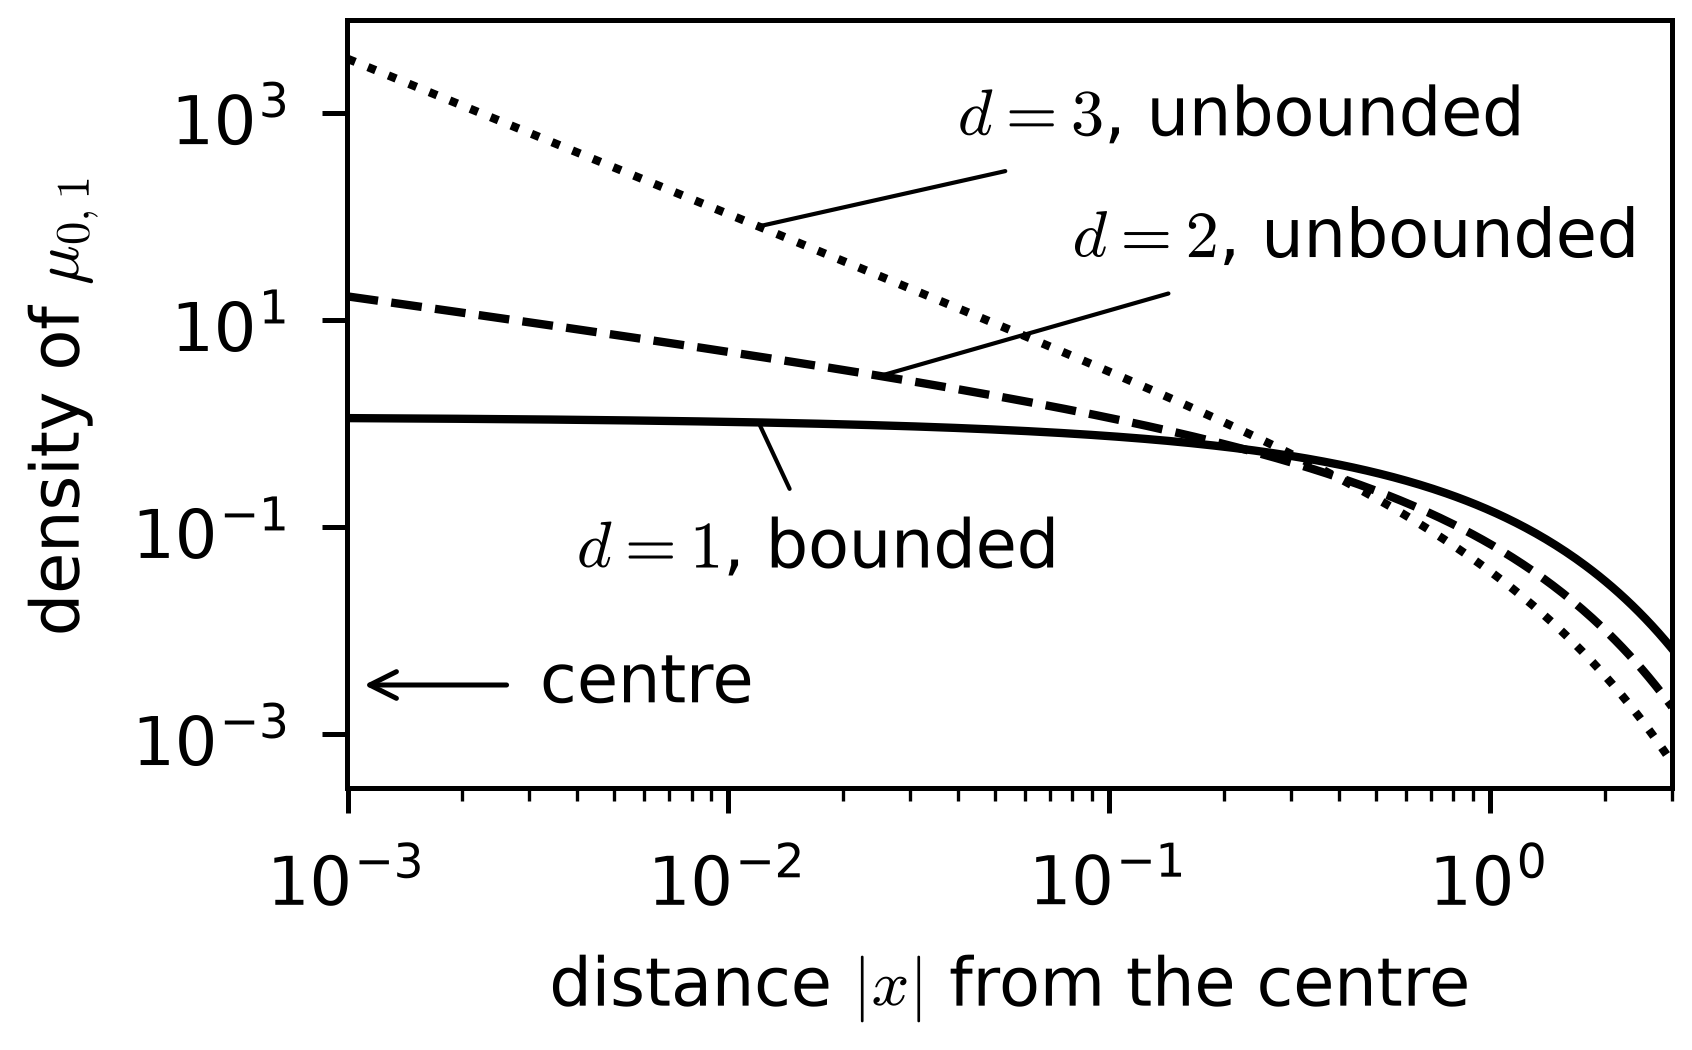
\includegraphics[width=0.45\textwidth]{fig-matern-centre.png}
\caption{The radial density of the \Matern{} kernel $\mu_{0,1}$ of index $\gamma = 3/4$ on
$\RR^d$, $d = 1, 2, 3$, on logarithmic axes, from its closed form \ref{eq:matern-density}. Here
$c = 3/2$. On the line the density is bounded and the curve levels off at the centre. In the
plane and in space it is unbounded, and the curve has the slope $c - d$ there, $-\tfrac12$ in
the plane and $-\tfrac32$ in space. Computed by a script deposited with the paper.}
\label{fig:matern-centre}
\end{figure}

% What the theorem decides comes first, and the comments on its clauses after it (the register
% review, flag 32). A kernel with a Gaussian part: F_d >= a|xi|^2/2, so the transform is
% integrable against every power, and C1 applies with every n.
% Q-0448 (the response to the second external round; records/affine/reviews/
% VERIFY-round2-mathematics.md, items 7 and 11b, and VERIFY-round2-length-and-exposition.md,
% section 4, item 7). The Gaussian part with its argument in full. Which clauses carry the result
% is said before the statement, with the formula of g_t, which clause (4) takes from a lemma of
% the supplement; that c > 0 only excludes the point mass.
The theorem decides boundedness for the kernels with no Gaussian part. A kernel with a Gaussian
part has a bounded smooth density in every dimension: the exponent of a datum $(a,k_d)$ is at
least $\tfrac12 a|\xi|^2$, so for $a > 0$ the transform is at most $e^{-a|\xi|^2/2}$, and C1
applies with every $n$. In clause (4), $g_t$ is the Gaussian density of variance $t$,
\[
  g_t(x) = (2\pi t)^{-d/2}e^{-|x|^2/2t} , \qquad x \in \RR^d ,\ t > 0 ,
\]
which the statement takes from Lemma~\ref{lem:positive-transform-origin} of \suppl. Here $t$ is
not a scale, and $\int g_t\,d\mu$ is the value at the centre of the kernel blurred by $g_t$.
% Q-0448, the blind draft review (flag 26): the comments on the clauses, which stood here
% before the reader had seen the statement, follow it.

% shared with blueprint thm:origin-boundedness-d
\begin{theorem}[the boundedness threshold in dimension $d$ is the dimension]\label{thm:origin-boundedness-d}
Let $d \ge 1$, let $(0, k_d)$ be an isotropic origin datum in dimension $d$ with Gaussian
coefficient $0$, let $\mu$ be its law, put $c := k_d(0{+}) \in [0,\infty]$ and suppose $c > 0$.
\begin{enumerate}
\item \emph{(The profile at the origin is a decay exponent.)} For every finite $\beta < c$ there
is $C_\beta < \infty$ with
\[
  \bigl|\widehat\mu(\xi)\bigr| \le C_\beta\,(1+|\xi|)^{-\beta}, \qquad \xi \in \RR^d .
\]
\item \emph{(Above the threshold: bounded, and a ladder of derivatives.)} Let $N \ge 0$ be an
integer. If $c > d + N$ then $\mu$ has a density of class $C^N$ on the whole of $\RR^d$, all of
whose partial derivatives of orders $0,\dots,N$ tend to $0$ at infinity. In particular $c > d$
makes the density continuous and bounded, and $c = \infty$ makes it $C^\infty$.
\item \emph{(At and below the threshold, on the subordinated slice: unbounded.)} Suppose the
datum is subordinated, with delay datum $(0,k_{\mathrm I})$ of exponent $F_{\mathrm I}$, that $W$
is a random delay whose law, a probability measure on $[0,\infty)$, has Laplace transform
$e^{-F_{\mathrm I}}$, and that $Z$ is standard normal on $\RR^d$, independent of $W$. Then
$c = 2\,k_{\mathrm I}(0{+})$, $W > 0$ almost surely, $\mu$ is the law of $\sqrt{W}Z$, and $\mu$
has the radial density
\begin{equation}\label{eq:mixture-density}
  p(x) = \int_0^\infty (2\pi u)^{-d/2}e^{-|x|^2/2u}\,\Pr(W \in du) .
\end{equation}
This $p$ is nonincreasing in $|x|$, and
\[
  \lim_{x \to 0} p(x) = (2\pi)^{-d}\int_{\RR^d}\widehat\mu(\xi)\,d\xi
   = \frac{(2\pi)^{-d/2}}{\Gamma(d/2)}\int_0^\infty \sigma^{d/2-1}e^{-F_{\mathrm I}(\sigma)}\,d\sigma ,
\]
finite exactly when $c > d$. If $c \le d$, then for every representative $q$ of $\mu$'s
density, every $\delta > 0$ and every $M$ there is an $x$ with $0 < |x| < \delta$ and
$q(x) > M$: no representative is bounded near the origin.
\item \emph{(At and below the threshold, for every datum: unbounded.)} Suppose $c \le d$. Then
$\int_{\RR^d}\widehat\mu(\xi)\,d\xi = \infty$, and there are no $\delta > 0$ and $M < \infty$ with
$\mu(B) \le M|B|$ for every Borel set $B \subseteq \{|x| < \delta\}$. In particular, for every
representative $q$ of a density of $\mu$, every $\delta > 0$ and every $M$ there is an $x$ with
$0 < |x| < \delta$ and $q(x) > M$. Quantitatively, with $g_t$ the heat kernel of
Lemma~\ref{lem:positive-transform-origin}, there is $C > 0$ with
\[
  \int_{\RR^d} g_t\,d\mu \ge C\,t^{-(d-c)/2} \quad (c < d), \qquad
  \int_{\RR^d} g_t\,d\mu \ge C\,\log\frac1t \quad (c = d), \qquad 0 < t \le 1 ,
\]
and for every $\beta$ with $0 < \beta < c$ there is $C'_\beta$ with
$\int g_t\,d\mu \le C'_\beta\,t^{-(d-\beta)/2}$ for all $t > 0$. And
$\log\int g_t\,d\mu / \log(1/t) \to (d-c)/2$ as $t \downarrow 0$.
\item \emph{(The dichotomy.)} The law $\mu$ has a density bounded near the origin, that is, a
density $q$ with $q(x) \le M$ whenever $|x| < \delta$, for some $\delta > 0$ and $M < \infty$,
exactly when $c > d$.
\end{enumerate}
\end{theorem}

% The laws of the theorem: Theorem thm:isotropic-classification with Lemma
% lem:isotropic-realisation and Proposition prop:isotropic-polar-reading(1) (the register
% review, flag 35: the sketch with C4 and C3 is gone). Why the threshold is the dimension: the
% value at the centre as the integral of the transform, the two bounds on the transform, and
% Lemma lem:positive-transform-origin(2), whose attribution to an observation of Feller is in
% Appendix A, where the lemma is stated.
By Theorem~\ref{thm:isotropic-classification} and
Proposition~\ref{prop:isotropic-polar-reading}, the laws of the theorem are the kernels from scale
zero with no Gaussian part, and they are all the rotation-invariant self-decomposable laws on
$\RR^d$ with no Gaussian part other than the point mass. The hypothesis $c > 0$ only
excludes the point mass: $k_d$ is nonincreasing, so $c$ is its supremum. The result is clause
(5), the threshold. Clauses (1) and (2) are its bounded side: the profile at the origin gives
the decay of the transform, and the decay gives the derivatives. Clause (4) is its unbounded
side, for every datum. Clause (3) is for the subordinated data, the Gaussian variance mixtures
whose mixing law is a delay law of \S\ref{sec:line-bridge}: it adds the density as an explicit
mixture, its value at the centre, and $c$ read off the delay profile,
$c = 2k_{\mathrm I}(0{+})$. $N$ continuous derivatives are enough
for the derivative filters of order up to $N$ built from the kernel to be bounded continuous
functions.

The threshold is the dimension for a reason that is seen in the frequency domain. The value at
the centre of a continuous density is $(2\pi)^{-d}\int_{\RR^d}\widehat\mu(\xi)\,d\xi$ when the
transform is integrable. For finite $c$ and large $|\xi|$ the transform lies between a constant
times $|\xi|^{-c}$ and, for every $\beta < c$, a constant times $|\xi|^{-\beta}$
(Lemma~\ref{lem:isotropic-exponent-log}(1) and clause (1)), so it is integrable exactly when
$c > d$. And a law with a nonnegative transform and a density bounded near the origin has an
integrable transform (Lemma~\ref{lem:positive-transform-origin}(2) of \suppl).

The theorem takes $c$ from the \Levy{} measure in dimension $d$. The corollary reads it, and the
Gaussian coefficient, off the exponent.

% shared with blueprint cor:origin-profile-exponent+a6748e79e77b
\begin{corollary}[the exponent determines the Gaussian coefficient and the profile at the origin]\label{cor:origin-profile-exponent}
Let $d \ge 1$, let $(a, k_d)$ be an isotropic origin datum in dimension $d$, let $F_d$ be its
exponent, and put $c := k_d(0{+}) \in [0,\infty]$.
\begin{enumerate}
\item \emph{(The Gaussian coefficient.)} $F_d(\xi)/|\xi|^2 \to \tfrac12 a$ as $|\xi| \to \infty$.
\item \emph{(The profile at the origin.)} As $|\xi| \to \infty$,
\[
  \frac{F_d(\xi) - \tfrac12 a|\xi|^2}{\log|\xi|} \to c ,
\]
where the limit is $+\infty$ when $c = \infty$. In particular, if $a = 0$ and $\mu$ is the datum's
law, then $-\log|\widehat\mu(\xi)|/\log|\xi| \to c$.
\item \emph{(The same numbers in every dimension.)} Let $d' \ge 1$, let $(a', k'_{d'})$ be an
isotropic origin datum in dimension $d'$ with exponent $F'_{d'}$, and suppose that the two exponents
are one function of the radius: there is a function $F$ on $[0,\infty)$ with $F_d(\xi) = F(|\xi|)$
for every $\xi \in \RR^d$ and $F'_{d'}(\xi') = F(|\xi'|)$ for every $\xi' \in \RR^{d'}$. Then
$a' = a$ and $k'_{d'}(0{+}) = k_d(0{+})$.
\end{enumerate}
\end{corollary}

% The consequence for the classes A_d is drawn from three numbered statements, each cited:
% Proposition prop:line-filtration(1) (the nesting), Proposition prop:isotropic-polar-reading (a
% member of A_d has a datum in dimension d) and clause (5) of the theorem.
For a datum with no Gaussian part, clause (2) is the reading of $c$ as the power at which the
transform falls off, and clause (3) removes the dimension. An exponent
$F \in \mathcal{A}_D$ belongs to $\mathcal{A}_d$ for every $d \le D$
(Proposition~\ref{prop:line-filtration}(1)), and in each of these dimensions $F(|\cdot|)$ is the
exponent of a datum (Proposition~\ref{prop:isotropic-polar-reading}). By clause (3) these data
have one Gaussian coefficient and one $c$, and clause (5) of the theorem holds in each of these
dimensions with that $c$. So a kernel that is bounded on the line can have a spike in the plane.

% The number c for the kernels a reader knows (the register review, flag 11; the scope audit,
% row 20: the stable kernels have c = infinity by Corollary cor:origin-profile-exponent applied
% to the exponent of Proposition prop:isotropic-bridge(3), and nothing else is used). Only what
% the statements give: the Gaussian's datum is (a, 0); for F(r) = 2^(-alpha) r^(2 alpha) with
% 2 alpha < 2, F/r^2 -> 0 gives a = 0 and F/log r -> infinity gives c = infinity; the Poisson
% kernel is 2 alpha = 1 (section 2.3); a member of a Cin ray has the folded profile
% b 1_(0,tau), and the unit member has c = 1 (Corollary cor:line-threshold(2)).
For the kernels that a reader knows, the number $c$ is as follows.
\begin{itemize}
\item The Gaussian has a Gaussian part, and no \Levy{} measure. It is outside the theorem, and
it is bounded and smooth.
\item The stable kernels of index $p < 2$ have an exponent that is a multiple of $r^p$
(Proposition~\ref{prop:isotropic-bridge}(3)). So $F(r)/r^2 \to 0$ and
$F(r)/\log r \to \infty$: by clauses (1) and (2) of the corollary they have no Gaussian part and
$c = \infty$, and they are smooth in every dimension, by clause (2) of the theorem. The Poisson
kernel of \S\ref{sec:line-bridge} is the case $p = 1$.
\item The \Matern{} kernel of index $\gamma$ has $c = 2\gamma$ (Example~\ref{ex:matern} below).
\item On the line the member $b\,\Cin(\tau|\omega|)$ of a $\Cin$ ray has the folded profile
$b\,\mathbf 1_{(0,\tau)}$, so $c = b$, and the unit member sits at the threshold
(Corollary~\ref{cor:line-threshold}(2)).
\end{itemize}

An unbounded density could be unbounded at many points. The next proposition says that it is
unbounded at the centre only: the density of every kernel from scale zero, with or without a
Gaussian part, is radially nonincreasing, and so finite at every positive radius.

% shared with blueprint prop:isotropic-radial-monotone+d19bc0659397
\begin{proposition}[the kernels from scale zero have a radially nonincreasing density]\label{prop:isotropic-radial-monotone}
Let $d \ge 1$.
\begin{enumerate}
\item Let $(\mu_{s,t})$ be an isotropic cascade family in dimension $d$ and let $t > 0$. Then
$\mu_{0,t}$ has a density $p$ with $p(x) = q(|x|)$ for $x \ne 0$, where
$q : (0,\infty) \to [0,\infty)$ is nonincreasing.
\item The same holds for the law of every isotropic origin datum $(a,k_d)$ in dimension $d$ that is
not trivial ($a > 0$, or $k_d$ not almost everywhere $0$).
\end{enumerate}
\end{proposition}

% The name a reader needs to use the statement, and no more (the register review, flag 18; the
% citation audit, note on row 39): the anchor is in section 3.5.
% Q-0448, the blind draft review (flag 16): Watanabe's case as the table of the sources has it,
% with its number, and Wolfe's part named apart from it (the proof of the proposition starts
% from C5; READING-watanabe1983isoperimetric.md, sections 1 to 3).
For the law at each time of a symmetric \Levy{} process whose Gaussian covariance is a multiple
of the identity and whose \Levy{} measure has a radially
nonincreasing density the statement is Watanabe's (\sscite{watanabe1983isoperimetric},
Proposition, p.~488; Table~\ref{tab:in-print}). The proof given here derives it from Wolfe's
theorem C5.

% Q-0448 (the response to the second external round; the author's decision of 2026-10-13 that
% nothing is stated twice; records/affine/reviews/VERIFY-round2-length-and-exposition.md,
% section 4, items 8 and 9). The rate is stated once in the main text, through the polar
% profile. The rate through the transform, prop:origin-rate-d, is a lemma of the supplement,
% from which the proof of the rate through the profile starts. The two statements from which
% the rate takes its constants, prop:isotropic-exponent-profile and
% lem:exponent-profile-constant, are stated here, before it, verbatim, with the markers and
% pins they had in Appendix A. The lead defines "varies slowly", "asymptotic" and the constant
% R(d,c) of the Riesz kernel, which the statements below take from that lemma.
The rest of the subsection gives the rate of the spike, computed from the \Levy{} measure. A
positive function $L$ \emph{varies slowly}
at infinity when $L(\lambda\rho)/L(\rho) \to 1$ as $\rho \to \infty$ for every $\lambda > 0$, as
a constant or a logarithm does, and at $0$ when the same holds as its argument decreases to
$0$. Two functions are \emph{asymptotic}, written $f \sim g$, when their quotient tends to $1$.
The density at distance $s$ from the centre is governed by the transform at the frequencies up
to about $1/s$. For the pure power $|\xi|^{-c}$ with $c < d$ this is exact: its inverse Fourier
transform is the Riesz kernel $R(d,c)\,|x|^{c-d}$, with
\[
  R(d,c) := \frac{\Gamma\bigl(\tfrac{d-c}{2}\bigr)}{2^{c}\,\pi^{d/2}\,\Gamma\bigl(\tfrac c2\bigr)} .
\]
The transform of a kernel with a finite $c$ need not be a constant times $|\xi|^{-c}$. The next
proposition says what it is asymptotic to: the power $|\xi|^{-c}$ times a constant and a factor $K(1/|\xi|)$
that varies slowly, both computed from the polar profile. The lemma after it gives in closed
form the one constant that depends on the dimension alone, $\varkappa_d$.

% shared with blueprint prop:isotropic-exponent-profile+f9bd366628e2
\begin{proposition}[the exponent at infinity through the polar profile]\label{prop:isotropic-exponent-profile}
Let $d \ge 1$, let $(0,k_d)$ be an isotropic origin datum in dimension $d$ with Gaussian
coefficient $0$ and $0 < c := k_d(0{+}) < \infty$, let $F_d$ be its exponent, put
$C_k := \int_1^\infty k_d(r)\,dr/r$, and let $e$ be a unit vector of $\RR^d$. Write
$\Cin(X) = \int_0^X (1 - \cos u)\,du/u$ and put
\[
  K(x) := \exp\Bigl[\int_x^1 \bigl(c - k_d(u)\bigr)\,\frac{du}{u}\Bigr] \qquad (0 < x \le 1) .
\]
\begin{enumerate}
\item \emph{(The factor.)} $K$ is continuous and nonincreasing on $(0,1]$, with
$1 = K(1) \le K(x) \le x^{-c}$. For every $a > 0$, $K(ax)/K(x) \to 1$ as $x \downarrow 0$; the
quotient is defined for $0 < x \le \min\{1, 1/a\}$. If $\int_0^1 (c - k_d(u))\,du/u < \infty$,
then $K(x)$ increases, as $x \downarrow 0$, to the finite limit
\[
  K(0{+}) := \exp\int_0^1 \bigl(c - k_d(u)\bigr)\,\frac{du}{u} \;\ge\; 1 .
\]
If the integral diverges, then $K(x) \to \infty$ as $x \downarrow 0$, and $K(0{+}) := \infty$.
\item \emph{(Two constants.)} The limit
\[
  g_\infty := \lim_{X\to\infty}\bigl(\Cin(X) - \log X\bigr)
\]
exists, and $-3 \le g_\infty \le \tfrac{13}{4}$. The function
$\eta \mapsto \log|\langle e,\eta\rangle|$ is integrable on $S^{d-1}$ for $\sigma_{d-1}$, and
\[
  \lambda_d := \frac{1}{|S^{d-1}|}\int_{S^{d-1}}\log|\langle e,\eta\rangle|\,\sigma_{d-1}(d\eta)
  \in (-\infty, 0]
\]
does not depend on $e$, with $\lambda_1 = 0$. Put $\varkappa_d := g_\infty + \lambda_d$.
\item \emph{(The exponent.)} As $\rho \to \infty$,
\[
  F_d(\rho e) - \bigl(c\log\rho - \log K(1/\rho) + C_k\bigr) \to c\,\varkappa_d ,
  \qquad\text{that is}\qquad
  \frac{e^{-F_d(\rho e)}}{e^{-C_k - c\varkappa_d}\,\rho^{-c}\,K(1/\rho)} \to 1 .
\]
Moreover, for every $\rho \ge 1$,
\[
  c\,(\lambda_d - 3) \;\le\; F_d(\rho e) - \bigl(c\log\rho - \log K(1/\rho) + C_k\bigr)
  \;\le\; \tfrac{13}{4}\,c .
\]
More generally, for every $\rho > 0$,
\[
  c\,(\lambda_d - 3) \;\le\; F_d(\rho e) - \int_{1/\rho}^{\infty}k_d(r)\,\frac{dr}{r}
  \;\le\; \tfrac{13}{4}\,c ,
\]
and for $\rho \ge 1$ the integral equals $c\log\rho - \log K(1/\rho) + C_k$.
\item \emph{(When the transform is comparable to a power.)} For every $\xi$ with $|\xi| \ge 1$,
\[
  e^{-13c/4 - C_k}\,K(1/|\xi|) \;\le\; |\xi|^{c}\,e^{-F_d(\xi)} \;\le\;
  e^{c(3-\lambda_d) - C_k}\,K(1/|\xi|) .
\]
So $|\xi|^{c}e^{-F_d(\xi)}$ is bounded on $\{|\xi| \ge 1\}$ if and only if
$\int_0^1 (c - k_d(u))\,du/u < \infty$, and then it tends to
$e^{-C_k - c\varkappa_d}\,K(0{+})$ as $|\xi| \to \infty$.
\end{enumerate}
\end{proposition}

% shared with blueprint lem:exponent-profile-constant+ab60b01e109d
\begin{lemma}[the constant of the exponent in closed form]\label{lem:exponent-profile-constant}
Let $\psi := \Gamma'/\Gamma$ be the digamma function on $(0,\infty)$ and
$\gamma_{\mathrm E} := -\psi(1) = -\Gamma'(1)$ Euler's constant. For an integer $d \ge 1$ let
$g_\infty$, $\lambda_d$ and $\varkappa_d = g_\infty + \lambda_d$ be the constants of
Proposition~\ref{prop:isotropic-exponent-profile}(2).
\begin{enumerate}
\item $g_\infty = \gamma_{\mathrm E}$.
\item $\lambda_d = \tfrac12\bigl[\psi(\tfrac12) - \psi(\tfrac d2)\bigr]$.
\item Hence
\[
  \varkappa_d = \gamma_{\mathrm E} + \tfrac12\bigl[\psi(\tfrac12) - \psi(\tfrac d2)\bigr]
   = \tfrac12\bigl(\gamma_{\mathrm E} - \psi(\tfrac d2)\bigr) - \log 2 ,
\]
so that $\varkappa_1 = \gamma_{\mathrm E}$, $\varkappa_2 = \gamma_{\mathrm E} - \log 2$,
$\varkappa_3 = \gamma_{\mathrm E} - 1$, and $\varkappa_{d+2} = \varkappa_d - 1/d$ for every
$d \ge 1$.
\item \emph{(The constants in closed form.)} For real numbers $c > 0$ and $C$,
\[
  e^{-C - c\varkappa_d}
   = 2^{c}\exp\Bigl(-C - \tfrac c2\bigl(\gamma_{\mathrm E} - \psi(\tfrac d2)\bigr)\Bigr) .
\]
Consequently, with $R(d,c)$ the constant of Lemma~\ref{prop:origin-rate-d}(1) for $0 < c < d$,
\[
  R(d,c)\,e^{-C - c\varkappa_d}
   = \frac{\Gamma\bigl(\tfrac{d-c}{2}\bigr)}{\pi^{d/2}\,\Gamma\bigl(\tfrac c2\bigr)}\,
     \exp\Bigl(-C - \tfrac c2\bigl(\gamma_{\mathrm E} - \psi(\tfrac d2)\bigr)\Bigr),
\]
and
\[
  (2\pi)^{-d}\,|S^{d-1}|\,e^{-C - d\varkappa_d}
   = \frac{2}{\pi^{d/2}\,\Gamma\bigl(\tfrac d2\bigr)}\,
     \exp\Bigl(-C - \tfrac d2\bigl(\gamma_{\mathrm E} - \psi(\tfrac d2)\bigr)\Bigr) .
\]
\end{enumerate}
\end{lemma}

The proposition has no hypothesis on $c$ against $d$, so it describes the transform above the
threshold as well. Of $g_\infty$ it uses only that the limit exists, with the bounds of clause
(2), and the lemma gives its value. When $c \le d$ the density follows the transform as the
Riesz kernel follows the pure power. For $c < d$ the density $q(s)$ at distance $s$ from the
centre is asymptotic, as $s \downarrow 0$, to $R(d,c)\,s^{-d}\,\widehat\mu(e/s)$, with $e$ a
unit vector. This step from the transform to the density is a Tauberian theorem,
Lemma~\ref{prop:origin-rate-d}(1) of \suppl, from which the statements here cite the constant
$R(d,c)$, and \S\ref{sec:isotropic-sources} says where it is in print. At $c = d$ the transform is at the edge of integrability, and an integral of $K$
takes the place of the power. In the statement $s$ is a distance from the centre, not a scale.
% Q-0448, the blind draft review of the split (flags 3 and 27): the paragraph states clause (1)
% of Lemma prop:origin-rate-d for the density, which the paper's reader does not have, and no
% longer clause (1) of the proposition below with a second definition of A.

% shared with blueprint prop:origin-rate-profile-d+2165aacf61aa
\begin{proposition}[the rate at the centre through the polar profile]\label{prop:origin-rate-profile-d}
Let $d \ge 1$, let $(0, k_d)$ be an isotropic origin datum in dimension $d$ with Gaussian
coefficient $0$, let $\mu$ be its law, and suppose that $c := k_d(0{+})$ satisfies $0 < c \le d$.
Let $C_k$, $K$ and $\varkappa_d$ be as in Proposition~\ref{prop:isotropic-exponent-profile}, let $|S^{d-1}|$
be the surface measure of the unit sphere and $V_d$ the volume of the unit ball, and put
\[
  A := e^{-C_k - c\,\varkappa_d} .
\]
The law $\mu$ has a density $p$ with $p(x) = q(|x|)$ for $x \ne 0$, where
$q : (0,\infty) \to [0,\infty)$ is nonincreasing. Let $q$ be any such function. All limits are as
$s \downarrow 0$.
\begin{enumerate}
\item \emph{(Below the threshold.)} Let $c < d$, let $R(d,c)$ be the constant of
Lemma~\ref{prop:origin-rate-d}(1), and put $Q := R(d,c)\,A$. Then
\[
  \frac{q(s)}{Q\,s^{c-d}\,K(s)} \to 1
  \qquad\text{and}\qquad
  \frac{\mu(\{|x| \le s\})}{Q\,|S^{d-1}|\,c^{-1}\,s^{c}\,K(s)} \to 1 .
\]
\item \emph{(When a pure power holds.)} Let $c < d$. If
$\int_0^1 (c - k_d(u))\,du/u < \infty$, then $q(s)\,s^{d-c} \to Q\,K(0{+})$, a finite positive
number, and there is $C < \infty$ with $q(s) \le C\,s^{c-d}$ for every $s > 0$. If the integral
diverges, then $q(s)\,s^{d-c} \to \infty$, and there is no such $C$.
\item \emph{(At the threshold.)} Let $c = d$, and put
\[
  \mathcal{L}(s) := \int_s^1 K(y)\,\frac{dy}{y} \quad (0 < s \le 1), \qquad
  B := (2\pi)^{-d}\,|S^{d-1}|\,A .
\]
Then
\[
  \frac{q(s)}{B\,\mathcal{L}(s)} \to 1
  \qquad\text{and}\qquad
  \frac{\mu(\{|x| \le s\})}{B\,V_d\,s^{d}\,\mathcal{L}(s)} \to 1 .
\]
Moreover $\log(1/s) \le \mathcal{L}(s) \le K(s)\log(1/s)$ for $0 < s \le 1$. If
$\int_0^1 (d - k_d(u))\,du/u < \infty$, then
\[
  \frac{\mathcal{L}(s)}{\log(1/s)} \to K(0{+})
  \qquad\text{and}\qquad
  \frac{q(s)}{\log(1/s)} \to B\,K(0{+}) ,
\]
both limits finite and positive. If the integral diverges, then
$\mathcal{L}(s)/\log(1/s) \to \infty$ and $q(s)/\log(1/s) \to \infty$.
\end{enumerate}
\end{proposition}

% After the statement: the closed forms of Q and B are the second and third displays of clause
% (4) of Lemma lem:exponent-profile-constant at C = C_k. The peak of the record of a point
% source is read once from the limits for the mass of a ball: mu({|x| <= s}) over V_d s^d, with
% |S^{d-1}| = d V_d ("the peak of the opening" until Q-0448; the second external round, review
% C, R2). The profile with an unbounded factor is the blind referee's, with K in closed form
% (records/affine/check-q0428-prose-values.py, part (b)). The dependence on the scale is a
% computation of the prose, listed as such in the supplement (the same script, part (g)).
% Q-0448, the blind draft review (flag 27): the closed forms of Q and B are the second and the
% third display of clause (4) of the lemma, at C = C_k (with c = d in the third), and are not
% displayed again.
Lemma~\ref{lem:exponent-profile-constant}(4) at $C = C_k$ gives $Q$ and $B$ in closed form.
So the kernel at its centre is computed from its \Levy{} measure: the power is $c - d$, the
factor $K(s)$ is one integral of the polar profile over $(s,1)$, and the constant depends on
$c$, on $d$ and on the profile beyond radius $1$. By clauses (2) and (3) the density is
asymptotic to a constant times $|x|^{c-d}$, or times $\log(1/|x|)$ at the threshold, exactly
when $K$ is bounded. The
limits for the mass of a ball give the peak of the record of a point source, the mass of the
recording cell divided by its volume. For a cell of radius $s$ round the centre it is
asymptotic to $(d/c)\,Q\,s^{c-d}K(s)$ for $c < d$ and to $B\,\mathcal{L}(s)$ for $c = d$,
because $|S^{d-1}| = d\,V_d$.

% Q-0448 (VERIFY-round2-length-and-exposition.md, section 4, item 9; the author's decision that
% nothing is stated twice): the example in one place, after the rate, where it had four (after
% the corollary, after each form of the rate, and in section 3.4). It names its delay law, so
% that the hypotheses of the clauses it uses are seen to be met. The closed form is Fischer et
% al., the display after (24), p. 241, at mu = theta = 0, s = gamma and Sigma = I
% (READING-fischer2025variance.md), and it is the mixture eq:mixture-density against the gamma
% law (records/affine/check-matern-rate-constants.py, part (a)). It is the Bessel kernel
% G_{2 gamma} of Aronszajn and Smith at range 1/sqrt 2, p(x) = 2^{d/2} G_{2 gamma}(sqrt 2 x), for
% every gamma > 0 ((4,1), p. 416; READING-aronszajn1961theory.md, section 3), and the two
% regimes at the centre are their (4,2), rescaled. The coefficient of the spike is read from
% the identity A K(0+) = 2^gamma, which holds because the transform is asymptotic both to
% A rho^(-c) K(1/rho) (Proposition prop:isotropic-exponent-profile(3)) and to
% 2^gamma rho^(-2 gamma); the rate through the transform is not needed. The numbers of the
% table: records/affine/check-q0448-matern-table.py, with its output beside it.
\begin{example}[the \Matern{} kernels]\label{ex:matern}
The \Matern{} kernel of index $\gamma > 0$ is the kernel from scale zero with exponent
$F(r) = \gamma\log(1 + r^2/2)$ (Proposition~\ref{prop:isotropic-bridge}(2)). Here
$F(r) = F_{\mathrm I}(r^2/2)$ with $F_{\mathrm I}(\sigma) = \gamma\log(1+\sigma)$, which is
causally admissible with delay profile $k_{\mathrm I}(u) = \gamma e^{-u}$, and its delay law is
the gamma law of shape $\gamma$, with density $u^{\gamma-1}e^{-u}/\Gamma(\gamma)$. So $F$ lies in
every $\mathcal{A}_d$ (Proposition~\ref{prop:line-filtration}(2)), its datum in each dimension
is subordinated (Lemma~\ref{lem:delay-polar-profile}), and clause (3) of
Theorem~\ref{thm:origin-boundedness-d} applies with a gamma-distributed $W$. It gives
$c = 2k_{\mathrm I}(0{+}) = 2\gamma$. So the kernel is bounded exactly when $\gamma > d/2$: for
$\gamma > \tfrac12$ on the line, for $\gamma > 1$ in the plane and for $\gamma > \tfrac32$ in
space. The mixture \ref{eq:mixture-density} is here, at scale $1$
(\sscite{fischer2025variance}, (24) and the display after it, p.~241),
\begin{equation}\label{eq:matern-density}
  p(x) = \frac{2}{(2\pi)^{d/2}\,\Gamma(\gamma)}
    \Bigl(\frac{|x|}{\sqrt2}\Bigr)^{\gamma - d/2} K_{\gamma - d/2}\bigl(\sqrt2\,|x|\bigr) ,
\end{equation}
with $K_\nu$ the modified Bessel function of the second kind. For $\gamma > d/2$ this is the
\Matern{} function of smoothness $\gamma - d/2$ and range $1/\sqrt2$ (\sscite{porcu2024matern},
(9) of the arXiv version), so the kernel is bounded exactly where it is a \Matern{} covariance
function. For every $\gamma > 0$ it is the Bessel kernel of potential theory, dilated by
$1/\sqrt2$ (\sscite{aronszajn1961theory}, (4,1), p.~416). The authors of the Bessel scale
space (\S\ref{sec:introduction}) note that the
kernel with $2\gamma = d + 1$ is continuous and not differentiable at the centre, and the kernel
with $2\gamma = d + 3$ twice continuously differentiable (\sscite{burgeth2005bessel}, p.~87).
The continuity and the two derivatives are the cases $N = 0$ and $N = 2$
of clause (2) of Theorem~\ref{thm:origin-boundedness-d}.
% Q-0448, the blind draft review (flags 12 and 37): which kernel of the Bessel scale space this
% is, is said once, in section 1; "not differentiable" is not a case of clause (2), which
% gives derivatives and is silent on the next one.

By \ref{eq:polar-profile-d} with the delay profile $\gamma e^{-u}$, the polar profile of the
kernel is
\[
  k_d(r) = \frac{4\gamma}{\Gamma(d/2)}\Bigl(\frac{r}{\sqrt2}\Bigr)^{d/2}K_{d/2}\bigl(\sqrt2\,r\bigr) ,
\]
which is $2\gamma e^{-\sqrt2\,r}$ on the line and $2\gamma(1 + \sqrt2\,r)e^{-\sqrt2\,r}$ in
space. For it the integral $\int_0^1 (c - k_d(u))\,du/u$ is finite, so the factor $K$ is
bounded, and for $\gamma < d/2$ the spike is a pure power
(Proposition~\ref{prop:origin-rate-profile-d}(2)). Its coefficient needs no integral. The
transform $(1 + \rho^2/2)^{-\gamma}$ is asymptotic to $2^{\gamma}\rho^{-2\gamma}$, and to
$A\,\rho^{-c}K(1/\rho)$ by Proposition~\ref{prop:isotropic-exponent-profile}(3), so
$A\,K(0{+}) = 2^{\gamma}$ in every dimension. Hence, as $x \to 0$,
\[
  p(x) \sim \frac{\Gamma(d/2 - \gamma)}{2^{\gamma}\pi^{d/2}\,\Gamma(\gamma)}\,|x|^{2\gamma - d}
  \quad \bigl(\gamma < \tfrac d2\bigr), \qquad
  p(x) \sim \frac{2}{(2\pi)^{d/2}\,\Gamma(d/2)}\,\log\frac{1}{|x|}
  \quad \bigl(\gamma = \tfrac d2\bigr) ,
\]
the coefficients being $Q\,K(0{+})$ and $B\,K(0{+})$. The second case is index $1$ in the
plane. Both are the behaviour of the closed form \ref{eq:matern-density} at the centre
(\sscite{aronszajn1961theory}, (4,2), p.~416, in the present scaling). Table~\ref{tab:matern}
has the numbers for $\gamma = 3/4$, the kernel of Figure~\ref{fig:matern-centre}.
\end{example}

\begin{table}[!htb]
\centering
\small
\begin{tabular}{@{}ccccccl@{}}
\toprule
$d$ & $c - d$ & $C_k$ & $K(0{+})$ & $A$ & $Q$ & the density at the centre \\
\midrule
$1$ & $\tfrac12$ & $0.171$ & $4.741$ & $0.355$ & & bounded, with $p(0) \approx 1.180$ \\
$2$ & $-\tfrac12$ & $0.359$ & $2.023$ & $0.831$ & $0.277$ & $p(x) \sim 0.560\,|x|^{-1/2}$ \\
$3$ & $-\tfrac32$ & $0.535$ & $1.524$ & $1.104$ & $0.0701$ & $p(x) \sim 0.107\,|x|^{-3/2}$ \\
\bottomrule
\end{tabular}
\caption{The \Matern{} kernel $\mu_{0,1}$ of index $\gamma = 3/4$, at scale $1$ in the gauge
$\chi(t) = t$, for which $c = 3/2$, in dimensions $1$,
$2$ and $3$: the constants of Propositions~\ref{prop:isotropic-exponent-profile}
and~\ref{prop:origin-rate-profile-d}, and the density at the centre. In each dimension
$A\,K(0{+}) = 2^{3/4}$. Computed by a script deposited with the paper.}
\label{tab:matern}
\end{table}

The factor need not be bounded. Let $0 < c < d$, and let $k_d(u) = c\,(1 - 1/(2 + \log(1/u)))$
for $0 < u \le 1$, continued beyond radius $1$ by a nonincreasing function with $C_k < \infty$.
The profile approaches $c$ like $1/\log(1/u)$, the integral diverges, and
$K(x) = (1 + \tfrac12\log(1/x))^{c}$. So $q(s) \sim Q\,s^{c-d}\,(1 + \tfrac12\log(1/s))^{c}$:
the spike exceeds every multiple of the pure power, by a power of a logarithm.

The statements are for one law, and a family has a kernel for each scale. The kernel from scale
zero to scale $t$ is the dilation of the law by $\chi(t)$, with density
$\chi(t)^{-d}\,p(x/\chi(t))$. For $c < d$ this is asymptotic at the centre to
$\chi(t)^{-c}\,Q\,|x|^{c-d}K(|x|)$, because $K$ varies slowly. So the power and the factor are
the same at every scale, and the constant is multiplied by $\chi(t)^{-c}$. The radius $1$ in $K$
and in $C_k$ is the unit of length at the scale where $\chi(t) = 1$.

% The two bounds are stated in Appendix A (Propositions prop:origin-lower-bound-d and
% prop:origin-upper-bound-d). The paragraph says what each gives that the rate does not, with
% its hypotheses, why the lower bound needs d >= 2 and what holds on the line, what the
% constants depend on, and that together they give the order (the register review, flag 30).
% The last two sentences keep c < d and c = d apart (the scope audit, row 3: at c = d a bound at
% the power c would be a bounded density, which Theorem thm:origin-boundedness-d(4) excludes).
% Q-0448, the blind draft review, the length: the paragraph keeps what each bound gives. What
% the appendix says after each statement (why the lower bound needs d >= 2, and the line) and
% what the comment on clause (2) of the rate says (when a bound at the power c itself holds)
% are not repeated here.
Two bounds complement the rate, and \S\ref{app:further-statements} states them. An
asymptotic equivalence gives no radius on which an inequality holds and no constant for it. For
$d \ge 2$ and a finite $c$ the kernel is bounded from below near its centre:
$\mu(E) \ge c_1\int_E |x|^{c-d}\,dx$ for every Borel set $E$ in a ball $\{|x| < \delta\}$, with
$\delta$ and $c_1$ given in terms of $d$, of $c$ and of the polar profile
(Proposition~\ref{prop:origin-lower-bound-d}). For $c \le d$ and every $\beta < c$ the
density is bounded from above at every radius: $q(s) \le (A_\beta/V_d)\,s^{\beta-d}$, with $V_d$
the volume of the unit ball and a constant $A_\beta$ that \suppl{} gives in closed form
(Proposition~\ref{prop:origin-upper-bound-d}; \S\ref{supp:proofs-origin}). For $d \ge 2$ and $c \le d$ the
two bounds together give the
order of the density at the centre, $\log p(x)/\log(1/|x|) \to d - c$ (its clause (3)).

% Q-0448, the blind draft review (flags 5 and 6): the lead says what a stage does to a record,
% in the two cases of the proposition; what was said "in plain words" after the statement is
% here, and the comment after the statement keeps what the lead does not say. The Matern case
% gamma = 1, which stood in Example ex:matern before the proposition was stated, follows it.
\paragraph{The stages.} The statements above are about the kernels from scale zero. A stage
$\mu_{s,t}$ with $s > 0$, which is what a cascade applies to a record, is a residual of such a
kernel (\S\ref{sec:line-axioms}), and need not be a dilation of it. When the kernels have no Gaussian
part and $c$ is finite, a stage does not blur everything. It returns the fraction
$(\chi(s)/\chi(t))^c$ of the record at scale $s$ unchanged, and adds a blur of that record by a
density of mass $1 - (\chi(s)/\chi(t))^c$. With a Gaussian part, or with $c = \infty$, as for
the stable kernels, a stage is a blur by a density.

% Q-0448 (review D, R1, of the second external round; records/affine/NODES-q0434.md, section 2;
% the author's decision of 2026-10-13 that the stages are machine-checked, by queue item
% Q-0447). One proposition for the three blueprint nodes of Q-0434 on the stages:
%   clause (1)  lem:isotropic-stage-levy-measure, for l = chi(s) and L = chi(t): its clause (1)
%               and its last sentence (the transform of the stage, the mass), which is the form
%               the node itself gives for a family; the node's statement for a datum and two
%               numbers 0 < l < L is the first paragraph of the proof;
%   clause (2)  prop:isotropic-stage-atom, its four clauses as the items (a) to (d);
%   clause (3)  prop:isotropic-stage-density, its three clauses as the items (a) to (c), and
%               its closing sentence, which closes the proposition.
% Nothing is added to the three statements and nothing of the second and third is left out.
% Pinned against the three nodes, statement and proof, after reading.
% Machine-checked since the Lean of Q-0447 was merged (the joining step of Q-0448): the three
% nodes are \leanok, the proposition is under the first list of section 1.1, its proof is in the
% supplement (supp-proofs.tex inputs proof-stages.tex), and it has an item in the list of
% section S4 and a row in the table of Appendix B (records/affine/gen-verification-table.py,
% ROWS; axioms-iso-all-declarations.py, TABLE1). The proofs of record's closing paragraphs,
% which Q-0447 rewrote, are not printed, as for every proof; the one sentence of them that is
% (after item (d) of clause (2)) follows the blueprint, and the marker is pinned again.
% shared with blueprint lem:isotropic-stage-levy-measure@db25bbbf95b6+26ef2b33d950, prop:isotropic-stage-atom@e901f7de9352+6df4676673ea, prop:isotropic-stage-density@83e3e3ecc9fb+ae42a1d0f900
\begin{proposition}[the stages of a cascade]\label{prop:isotropic-stages}
Let $d \ge 1$, let $(\mu_{s,t})_{0 \le s \le t}$ be an isotropic cascade family in dimension $d$,
and let $\chi$ be a gauge and $F \in \mathcal{A}_d$ with $F \not\equiv 0$ that satisfy
\ref{eq:isotropic-classification} (Theorem~\ref{thm:isotropic-classification}). Let $(a, k_d)$ be
an isotropic origin datum in dimension $d$ with exponent $\xi \mapsto F(|\xi|)$, put
$c := k_d(0{+}) \in [0,\infty]$, let $0 < s < t$, and put
$\lambda := \chi(s)/\chi(t) \in (0,1)$. The \emph{\Levy{} measure of the stage} is the measure
$\nu_{s,t}$ on $\RR^d \setminus \{0\}$ with the density
$\kappa_{s,t}(|x|)\,\bigl(|S^{d-1}|\,|x|^d\bigr)^{-1}$, where
\[
  \kappa_{s,t}(r) := k_d\Bigl(\frac{r}{\chi(t)}\Bigr) - k_d\Bigl(\frac{r}{\chi(s)}\Bigr)
  \qquad (r > 0) .
\]
\begin{enumerate}
\item \emph{(The \Levy{} measure of a stage.)} $\kappa_{s,t} \ge 0$, the measure $\nu_{s,t}$ is
rotation invariant, and $\int_{\RR^d}(|x|^2 \wedge 1)\,\nu_{s,t}(dx) < \infty$. The transform of
the stage is
\begin{equation}\label{eq:stage-transform}
  \widehat\mu_{s,t}(\xi) = \exp\Bigl[-\tfrac12 a\bigl(\chi(t)^2 - \chi(s)^2\bigr)|\xi|^2
     - \int_{\RR^d}\bigl(1 - \cos\langle\xi,x\rangle\bigr)\,\nu_{s,t}(dx)\Bigr],
  \qquad \xi \in \RR^d ,
\end{equation}
and $\nu_{s,t}(\RR^d \setminus \{0\}) = c\,\log\bigl(\chi(t)/\chi(s)\bigr)$, in $[0,\infty]$. So
$\nu_{s,t}$ is a finite measure exactly when $c < \infty$.
\item \emph{(No Gaussian part and a finite $c$: a point mass at the centre.)} Suppose that
$a = 0$ and that $c$ is finite, and put $m := c\,\log(\chi(t)/\chi(s))$. Then $c > 0$, and:
\begin{enumerate}
\item[(a)] \emph{(The stage is compound Poisson.)}
$\mu_{s,t} = e^{-m}\sum_{n \ge 0}\nu_{s,t}^{*n}/n!$, with $\nu_{s,t}^{*0} = \delta_0$, and
$e^{-m} = \lambda^c$.
\item[(b)] \emph{(A point mass at the centre and a smoothing part.)} The measure
$\eta_{s,t} := \lambda^c\sum_{n \ge 1}\nu_{s,t}^{*n}/n!$ is absolutely continuous with respect
to Lebesgue measure, of total mass $1 - \lambda^c$, and
\[
  \mu_{s,t} = \lambda^c\,\delta_0 + \eta_{s,t} .
\]
So $\mu_{s,t}(\{0\}) = (\chi(s)/\chi(t))^c \in (0,1)$, and $\mu_{s,t}$ has no density.
\item[(c)] \emph{(The operator.)} With $p_{s,t} \ge 0$ a density of $\eta_{s,t}$, an integrable
function of integral $1 - \lambda^c$, the operator of the stage is
\[
  \mu_{s,t} * f = \Bigl(\frac{\chi(s)}{\chi(t)}\Bigr)^{c} f + p_{s,t} * f ,
  \qquad f \in L^1(\RR^d) .
\]
\item[(d)] \emph{(Not self-decomposable.)} $\mu_{s,t}$ is not self-decomposable.
\end{enumerate}
\item \emph{(Infinitely divisible; the stages with a density.)}
\begin{enumerate}
\item[(a)] $\mu_{s,t}$ is infinitely divisible and has the generating triplet
$\bigl(a(\chi(t)^2 - \chi(s)^2)\,I,\ \nu_{s,t},\ 0\bigr)$: its Gaussian part has the variance
$a(\chi(t)^2 - \chi(s)^2)$ in every direction, and its \Levy{} measure has the polar profile
$\kappa_{s,t}$ and the mass $c\,\log(\chi(t)/\chi(s))$.
\item[(b)] If $a = 0$ and $c = \infty$, then $\mu_{s,t}$ is absolutely continuous with respect
to Lebesgue measure. In particular it has no point mass.
\item[(c)] If $a > 0$, then $\mu_{s,t}$ has a bounded density of class $C^\infty$, all of whose
partial derivatives are bounded.
\end{enumerate}
\end{enumerate}
So a stage $\mu_{s,t}$ with $0 < s < t$ has a point mass at the centre exactly when the datum
has no Gaussian part and a finite profile at the origin, and it has a density in the two other
cases.
\end{proposition}

Clauses (1) and (3) give the stage as a law: it is infinitely divisible, and its \Levy{}
measure is the difference of two dilations of that of the kernel. The fraction of clause (2) tends to $0$
as $s \downarrow 0$, and the kernels from scale zero have no point mass. The number $c$, the
ratio $\chi(t)/\chi(s)$ and the product $a\,\chi(t)^2$ are the same for every pair
$(\chi, F)$ of the family, by the uniqueness clause of
Theorem~\ref{thm:isotropic-classification}. For the \Matern{} kernels of
Example~\ref{ex:matern}, in the gauge $\chi(t) = t$ of
Proposition~\ref{prop:isotropic-bridge}, the fraction is $(s/t)^{2\gamma}$. At $\gamma = 1$ the
stage is $\mu_{s,t} = (s/t)^2\delta_0 + (1 - (s/t)^2)\,\mu_{0,t}$ in every dimension, a point
mass and a multiple of the kernel at scale $t$: its transform is
$(1 + s^2\sigma)/(1 + t^2\sigma) = (s/t)^2 + (1 - (s/t)^2)/(1 + t^2\sigma)$ at
$\sigma = |\xi|^2/2$.

\subsection{The dimension filtration}\label{sec:isotropic-filtration}

% Q-0428, the fixes round (records/affine/REPOSITIONING-paper-iso-round2-fixes.md; the register
% review of sections 3.3 to 4, structural change 3). The subsection states what it quotes, once.
% Three statements: the dictionary (prop:radial-dictionary, with what it is in words before it and
% the Matern exponent put through it after it); the test on the Levy measure
% (prop:profile-one-dimension-down, the node that Q-0429 split from the corollary: statements on
% data, no law and no characteristic function), with its two readings in the dictionary
% (cor:dictionary-filtration, the label kept, the statement now those readings only); and the
% separating family (def:filtration-thresholds, then thm:separating-family-critical-values, the
% node of Q-0429 that carries "F^(w) in A_D iff w <= w_D", the strict decrease and the limit).
% thm:filtration-strict and thm:no-cin-ray-in-the-plane are not printed since Q-0448 (section S4
% of the supplement lists their declarations): they are the same facts as the new theorem on
% another footing and as clause (3) of the new proposition. One word per sense: "dimension" for a place in the chain, "step" for the
% profile b 1_(0,tau), "bump" for the box on [1,2] of the separating family.
% Attribution is in section 3.5 (sources.tex), once.
In every dimension an isotropic family is given by the same kind of object, a gauge and an
exponent $F$, a function of one variable: the transform of its kernel from scale zero is
$e^{-F(\chi(t)|\xi|)}$ (Theorem~\ref{thm:isotropic-classification}). The familiar families use one
exponent in every dimension. The Gaussian has $F(r) = \tfrac12 r^2$, and the $\alpha$-scale
spaces, which are written on $\RR^d$ \sscite{duits2004axioms}, have a multiple of
$r^{2\alpha}$ (Proposition~\ref{prop:isotropic-bridge}(3)). This subsection asks whether that is
general. Does the exponent of a family in dimension $d$ give a family in dimension $d + 1$ when
it is read as a function of $|\xi|$? By Theorem~\ref{thm:isotropic-classification} and
Lemma~\ref{lem:isotropic-realisation}, the exponents of the isotropic families in dimension $d$
are exactly the members $F \not\equiv 0$ of the class $\mathcal{A}_d$ of
Proposition~\ref{prop:line-filtration}. The way down is always open, since
$\mathcal{A}_{d+1} \subseteq \mathcal{A}_d$. The way up is not: in every dimension some exponents
are lost. The exponents admitted in every dimension are exactly those of the subordinated
families of \S\ref{sec:line-bridge} (Proposition~\ref{prop:line-filtration}(3)), the \Matern{}
and the stable kernels among them (Proposition~\ref{prop:isotropic-bridge}).

The subsection has three parts. The first matches the exponents of the kernels with no
Gaussian part and a finite $c$ with probability laws on $\RR^d$, and says which of them are
admitted one dimension up. The second is a test on the \Levy{} measure, for every exponent,
with what becomes of the simplest exponent that fails it. The third follows one family of
exponents through the dimensions.

% What the dictionary is, in words, before the statement (the register review, flag 4), and what
% each condition on the law does in terms of the polar profile (flag 28). k_d/c is nonincreasing,
% tends to 1 at radius zero and to 0 at infinity (the second integrability condition of
% Definition def:isotropic-origin-datum); the statement has Pr(|X| > r) = k_d(r+)/c. E log^+ R
% = int_1^infty Pr(R > r) dr/r, by Tonelli. An atom of mass p at the origin changes (c, the law)
% to (c(1 - p), the law conditioned off the origin) and leaves F unchanged (the node's
% annotation, point (iv) of the comment before it). Omega_2 = J_0 and Omega_3(t) = sin t / t:
% records/affine/check-q0428-prose-values.py, part (d).
The first statement is for the kernels of \S\ref{sec:isotropic-origin} with no Gaussian part
and a finite $c$. Their exponents are the members of $\mathcal{A}_d$ that grow like a logarithm,
$F(r)/\log r \to c$ with $0 < c < \infty$ (Corollary~\ref{cor:origin-profile-exponent}). The
\Matern{} kernels are among them, and the Gaussian and the stable kernels are not. Let $k_d$ be
the polar profile of such a kernel. The function $k_d/c$ decreases from $1$ at radius zero to
$0$ at infinity, so it is, up to its values at its jumps, the tail $r \mapsto \Pr(R > r)$ of a
random radius $R > 0$. Let $X$ be that radius in a direction drawn uniformly from the sphere.
The transform of the law of $X$ is a function $\phi(|\xi|)$ of the radius alone, a
\emph{radial characteristic function} on $\RR^d$. Read as a function of a displacement, it is
equally an isotropic correlation function that is valid in $\RR^d$. The proposition says that
$F$ and the pair $(c, \phi)$ determine each other, and that $F$ is admitted one dimension up
exactly when the same function of the radius is still the transform of a probability law on
$\RR^{d+1}$.

In the statement $\Omega_d(t)$ is the mean of $\cos(t\langle e,\eta\rangle)$ over the unit
sphere, the transform along a ray of the uniform law on the sphere: $\Omega_1 = \cos$,
$\Omega_2 = J_0$, the Bessel function of order zero, and $\Omega_3(t) = \sin t/t$. A random
vector $X$ stands for its law, and $\log^+ := \max\{\log, 0\}$. Two conditions are put on the
law. The first, $\mathbb{E}\log^+|X| < \infty$, a \emph{finite logarithmic moment}, is the
condition $\int_1^\infty k_d(r)\,dr/r < \infty$ of Definition~\ref{def:isotropic-origin-datum},
because $\mathbb{E}\log^+|X| = \int_1^\infty \Pr(|X| > r)\,dr/r$. The second, no atom at the
origin, makes $k_d(0{+}) = c$: an atom of mass $p$ there would give the same $F$ with
$c(1-p)$ in place of $c$, so the condition is what makes the pair unique.

% shared with blueprint prop:radial-dictionary+675deea1f81e
\begin{proposition}[the dictionary between $\mathcal{A}_d$ and the radial characteristic functions]\label{prop:radial-dictionary}
Let $d \ge 1$. For $t \ge 0$ put
\[
  \Omega_d(t) := \frac{1}{|S^{d-1}|}\int_{S^{d-1}}\cos\bigl(t\langle e,\eta\rangle\bigr)\,
     \sigma_{d-1}(d\eta) ,
\]
which does not depend on the unit vector $e$; $\Omega_1 = \cos$. Call a random vector $X$ in
$\RR^d$ \emph{rotation invariant} when $QX$ has the law of $X$ for every $Q \in \Orth(d)$. Its
characteristic function is then real and radial,
\[
  \mathbb{E}\,e^{i\langle\xi,X\rangle} = \phi(|\xi|), \qquad
  \phi(r) := \mathbb{E}\,\Omega_d\bigl(r|X|\bigr) \quad (r \ge 0) ,
\]
the function $\phi$ determines the law of $X$, and $X$ has the law of $R\,U$, where $R$ has the
law of $|X|$ and $U$ is uniformly distributed on $S^{d-1}$ and independent of $R$.
\begin{enumerate}
\item \emph{(From a law to an exponent.)} Let $X$ be a rotation-invariant random vector in
$\RR^d$ with $\Pr(X = 0) = 0$, let $\phi$ be as above, and let $0 < c < \infty$. Then
$\int_0^1 (1 - \phi(u))\,du/u < \infty$ if and only if $\mathbb{E}\log^+|X| < \infty$. In that
case the function
\[
  F(r) := c\int_0^r \bigl(1 - \phi(u)\bigr)\,\frac{du}{u} \qquad (r \ge 0)
\]
belongs to $\mathcal{A}_d$: $\xi \mapsto F(|\xi|)$ is the exponent of the isotropic origin datum
$(0,k_d)$ in dimension $d$ with $k_d(r) = c\,\Pr(|X| > r)$. Its profile at the origin is
$k_d(0{+}) = c$, and $F(r)/\log r \to c$ as $r \to \infty$.
\item \emph{(From an exponent to a law.)} Conversely, let $F \in \mathcal{A}_d$ and suppose that
$F(r)/\log r$ has a limit $c \in (0,\infty)$ as $r \to \infty$. Then $F$ is the function of
clause (1) for this $c$ and for a rotation-invariant $X$ with $\Pr(X = 0) = 0$ and
$\mathbb{E}\log^+|X| < \infty$, whose law is unique. Moreover $F$ is continuously differentiable
on $(0,\infty)$, with
\[
  \phi(r) = 1 - \frac{r\,F'(r)}{c} \quad (r > 0), \qquad
  \Pr(|X| > r) = \frac{k_d(r{+})}{c} \quad (r > 0)
\]
for every isotropic origin datum $(0,k_d)$ in dimension $d$ with exponent $\xi \mapsto F(|\xi|)$.
So $(c, \text{the law of } X) \mapsto F$ is a bijection from the pairs of clause (1) with
$\mathbb{E}\log^+|X| < \infty$ onto the set of the $F \in \mathcal{A}_d$ for which $F(r)/\log r$
has a limit in $(0,\infty)$. These are the members of $\mathcal{A}_d$ with Gaussian coefficient
$0$ and profile at the origin in $(0,\infty)$.
\item \emph{(The next dimension.)} Let $F$, $c$, $X$ and $\phi$ be as in clause (1), with
$\mathbb{E}\log^+|X| < \infty$. Then $F \in \mathcal{A}_{d+1}$ if and only if
$\zeta \mapsto \phi(|\zeta|)$, $\zeta \in \RR^{d+1}$, is the characteristic function of a random
vector $X'$ in $\RR^{d+1}$. Every such $X'$ is rotation invariant, with $\Pr(X' = 0) = 0$ and
$\mathbb{E}\log^+|X'| < \infty$, its first $d$ coordinates have the law of $X$, and $F$ is the
function of clause (1) in dimension $d + 1$ for the same $c$ and for $X'$.
\end{enumerate}
\end{proposition}

% The Matern exponent through the dictionary (the register review, flag 4): phi(r) =
% 1 - r F'(r)/c = 1 - (r^2/2)/(1 + r^2/2) = (1 + r^2/2)^(-1), and the tail of the radius of the
% Matern kernel of index 1 on the line is e^(-sqrt 2 r), so that 2 gamma times it is the folded
% profile of section 2.4 at range 1/sqrt 2 (records/affine/check-q0428-prose-values.py, part
% (c)). The classes of Schoenberg and their strictness: section 3.5 has the anchors.
% Q-0448, the blind draft review (flag 31): the two sentences that restated clause (2) of the
% proposition directly after it are gone.
For the \Matern{} exponent $F(r) = \gamma\log(1 + r^2/2)$, with $c = 2\gamma$, clause (2) gives
\[
  \phi(r) = 1 - \frac{rF'(r)}{2\gamma} = \Bigl(1 + \frac{r^2}{2}\Bigr)^{-1} ,
\]
the transform of the \Matern{} kernel of index $1$. By the same clause the polar profile of the
\Matern{} kernel
of index $\gamma$ is $2\gamma$ times the tail of the radius of the \Matern{} kernel of index $1$,
which on the line is $e^{-\sqrt2\,r}$. The radial functions that are
characteristic functions on $\RR^m$ form classes that decrease as $m$ grows, the classes of
Schoenberg (\sscite{schoenberg1938metric}, \S2.1 and Thm.~2, pp.~816--817), and they decrease
strictly in
every dimension (\sscite{gneiting1999radial}, p.~94). By
clause (3) a function of the class of $\RR^d$ that is not in the class of $\RR^{d+1}$ serves as
$\phi$ and gives an exponent in $\mathcal{A}_d$ and not in $\mathcal{A}_{d+1}$, when its law has
no atom at the origin and a finite logarithmic moment.

% The second statement: the node prop:profile-one-dimension-down of Q-0429. Its clause (1) cites
% the blueprint node prop:isotropic-polar-classification(2), the blueprint's split of clause (2)
% of prop:isotropic-polar-reading, which this paper prints whole; so the copy says Proposition
% prop:isotropic-polar-reading(2), and the statement is pinned for that reason
% (records/affine/transcribe-q0428-nodes.py, LABEL_MAP). "Shadow" is glossed here, where it is
% first used (the register review, flag 20), and what a jump is for a kernel (flag 21).
The second statement needs no law and no characteristic function, and it holds for every
exponent, with or without a Gaussian part. It follows the \Levy{} measure one dimension down.
The \emph{shadow} of a rotation-invariant \Levy{} measure on $\RR^{d+1}$ is its image under the
projection onto $\RR^d$, restricted to $\RR^d \setminus \{0\}$. The polar profile of the shadow
is an average of the profile
upstairs over the radii at least as large (Lemma~\ref{lem:shadow-polar-profile}), and such an
average is continuous. So a polar profile with a jump, which belongs to a \Levy{} density with
a jump at that radius, is the shadow of nothing.

% shared with blueprint prop:profile-one-dimension-down@fe01b96e0cf9+58ff7a6e5cbc
\begin{proposition}[the profile one dimension down; the step datum; the $\Cin$ rays]\label{prop:profile-one-dimension-down}
Let $d \ge 1$.
\begin{enumerate}
\item \emph{(The profile one dimension down is continuous.)} Let $F \in \mathcal{A}_{d+1}$, and
let $(a',k')$ be an isotropic origin datum in dimension $d + 1$ with exponent
$\zeta \mapsto F(|\zeta|)$; there is one, by Proposition~\ref{prop:isotropic-polar-reading}(2). Then
$F \in \mathcal{A}_d$, and every isotropic origin datum
$(a,k_d)$ in dimension $d$ with exponent $\xi \mapsto F(|\xi|)$ has $a = a'$ and
\[
  k_d(r) = \frac{|S^{d-1}|}{|S^{d}|}\int_{\RR} k'\bigl(r\sqrt{1+u^2}\bigr)\,(1+u^2)^{-(d+1)/2}\,du
  \qquad\text{for every } r > 0 .
\]
In particular $k_d$ is continuous on $(0,\infty)$. So if $F \in \mathcal{A}_d$ and some isotropic
origin datum in dimension $d$ with exponent $\xi \mapsto F(|\xi|)$ has a polar profile with a
discontinuity, then $F \notin \mathcal{A}_{d+1}$.
\item \emph{(Strictness at every step, with a witness.)} Let $b > 0$ and $\tau > 0$. Then
$(0, b\,\mathbf 1_{(0,\tau)})$ is an isotropic origin datum in dimension $d$, and its exponent is
radial: it is $\xi \mapsto G(|\xi|)$ for a function $G$ on $[0,\infty)$. This $G$ belongs to
$\mathcal{A}_d \setminus \mathcal{A}_{d+1}$. Hence $\mathcal{A}_{d+1} \subsetneq \mathcal{A}_d$
for every $d \ge 1$.
\item \emph{(The $\Cin$ rays.)} At $d = 1$, $G(r) = b\,\Cin(\tau r)$. So no $\Cin$ ray belongs
to $\mathcal{A}_2$, nor to $\mathcal{A}_D$ for any $D \ge 2$.
\end{enumerate}
\end{proposition}

% The arccos example is the shadow on the line of the step of the plane: C_1 = 1/pi, and
% (b/pi) int 1{r sqrt(1+u^2) < tau} du/(1+u^2) = (2b/pi) arctan sqrt(tau^2/r^2 - 1)
% = (2b/pi) arccos(r/tau) (records/affine/check-q0428-prose-values.py, part (e)).
Clause (1) is a test that needs one dimension only: an exponent of $\mathcal{A}_d$ whose polar
profile there has a jump is admitted in no higher dimension. For example, the step
$b\,\mathbf 1_{(0,\tau)}$ of the plane has on the line the shadow $(2b/\pi)\arccos(r/\tau)$ on
$(0,\tau)$, which falls continuously from $b$ to $0$: one projection removes the sharp edge. The
converse of the test fails, since the family below has smooth profiles and still leaves the
classes. Clause (2) makes the simplest datum a \emph{witness} in every dimension, an exponent
that is admitted there and not one dimension up. Clause (3) is about the $\Cin$ rays, the
elementary exponents of \S\ref{sec:introduction}, whose folded profile is a single step
(Proposition~\ref{prop:line-extreme-rays}). Every member of $\mathcal{A}_2$ is an exponent of
the line, and so still a superposition of them and of a Gaussian term. What the clause excludes
is a $\Cin$ ray
taken alone, which is the exponent of no isotropic family in the plane or in any higher
dimension.
% Q-0448, the blind draft review (flag 21): the passage repeated the third answer of section 1
% nearly word for word. Section 1 keeps the two sentences of the author's section review of
% 2026-10-12; here the first of them is said in one clause, with its reason (a member of A_2
% is admissible on the line, Proposition prop:line-filtration(1)), and the second is unchanged.

% The two readings of the proposition in the dictionary are Corollary cor:dictionary-filtration,
% which is stated in Appendix A beside its proof (the length of the main text).
Read in the dictionary, the first two clauses say the following
(Corollary~\ref{cor:dictionary-filtration}, in \S\ref{app:print-proofs}). The law that the
dictionary matches with an exponent admitted one dimension up has a radius with no atom. And
the law that it matches with the step datum is the uniform law on the sphere of radius $\tau$,
whose radius is an atom, so $\zeta \mapsto \Omega_d(\tau|\zeta|)$ is
not a characteristic function on $\RR^{d+1}$: the function $\cos(\tau|\zeta|)$ is not the
transform of a probability law in the plane, nor $J_0(\tau|\zeta|)$ of one in space.
% Q-0448, the blind draft review (flag 30): the shadow is defined as a measure, as Lemma
% lem:shadow-polar-profile(3) has it, and the vector X of the dictionary is the law that the
% dictionary matches with an exponent, not a property of the kernel.

% Q-0448 (review D, R2, of the second external round; records/affine/NODES-q0434.md, section
% 3): the blueprint node prop:step-exponent-dimensions of Q-0434, verbatim. Proved in print, as
% the dictionary is, with whose function Omega_d it is stated: it is in the second list of
% section 1.1 and its proof is in section A.4. The question "The step witnesses" has left
% section 4.1.
The step datum is excluded from the next dimension as the exponent of a cascade. It remains the
exponent of an infinitely divisible law there, and in exactly one dimension more.

% shared with blueprint prop:step-exponent-dimensions+992a08ec7dcc
\begin{proposition}[the step exponent one and two dimensions up]\label{prop:step-exponent-dimensions}
Let $d \ge 1$, $b > 0$ and $\tau > 0$. For an integer $n \ge 1$ let $\Omega_n$ be the function of
Proposition~\ref{prop:radial-dictionary} in dimension $n$, and put
\[
  G_n(\rho) := b\int_0^\tau \bigl(1 - \Omega_n(r\rho)\bigr)\,\frac{dr}{r} \qquad (\rho \ge 0) ,
\]
so that $\xi \mapsto G_n(|\xi|)$, $\xi \in \RR^n$, is the exponent of the step datum
$(0, b\,\mathbf 1_{(0,\tau)})$ in dimension $n$ (Corollary~\ref{cor:dictionary-filtration}(2), in whose
form the substitution $r = \tau u/\rho$ puts the integral). Write
$G := G_d$. It is the function of Proposition~\ref{prop:profile-one-dimension-down}(2), and by that clause
with the nesting of the classes, $G \in \mathcal{A}_D$ exactly when $D \le d$. Say that a
function $\psi \ge 0$ on $\RR^D$ is \emph{the exponent of an infinitely divisible law} when
$e^{-\psi}$ is the characteristic function of an infinitely divisible probability measure on
$\RR^D$.
\begin{enumerate}
\item \emph{(Exactly two dimensions more.)} Let $D \ge 1$ be an integer. The function
$\zeta \mapsto G(|\zeta|)$, $\zeta \in \RR^D$, is the exponent of an infinitely divisible law on
$\RR^D$ if and only if $D \le d + 2$.
\item \emph{(Dimension $d + 2$.)} For every $\rho \ge 0$,
\begin{equation}\label{eq:step-exponent-two-up}
  G_d(\rho) = G_{d+2}(\rho) + \frac{b}{d}\bigl(1 - \Omega_{d+2}(\tau\rho)\bigr) .
\end{equation}
So the infinitely divisible law on $\RR^{d+2}$ with exponent $\zeta \mapsto G(|\zeta|)$ is the
convolution of the law of the step datum $(0, b\,\mathbf 1_{(0,\tau)})$ of dimension $d + 2$ with
the compound Poisson law $e^{-b/d}\sum_{n \ge 0}(b/d)^n\sigma_\tau^{*n}/n!$, where $\sigma_\tau$
is the uniform probability measure on the sphere of radius $\tau$ of $\RR^{d+2}$: jumps at the
rate $b/d$, uniformly distributed on that sphere. Its generating triplet is
$(0,\ \nu^{\mathrm{step}}_{d+2} + \tfrac{b}{d}\,\sigma_\tau,\ 0)$, with $\nu^{\mathrm{step}}_{d+2}$
the \Levy{} measure of that step datum.
\item \emph{(Dimension $d + 1$.)} The infinitely divisible law on $\RR^{d+1}$ with exponent
$\zeta \mapsto G(|\zeta|)$ has the generating triplet $(0, \nu', 0)$, where $\nu'$ is the
rotation-invariant measure on $\RR^{d+1} \setminus \{0\}$ with the density
$k'(|z|)\,(|S^{d}|\,|z|^{d+1})^{-1}$ and
\[
  k'(s) := 2b\,C_{d+1}\Bigl[J_{d+2}\Bigl(\frac{\tau}{s}\Bigr)
     + \frac{1}{d}\Bigl(\frac{s}{\tau}\Bigr)^{d}\frac{s}{\sqrt{\tau^2 - s^2}}\Bigr]
  \quad (0 < s < \tau), \qquad k'(s) := 0 \quad (s \ge \tau) ,
\]
with $J_n(x) := \int_1^x v^{1-n}(v^2-1)^{-1/2}\,dv$ for $x \ge 1$ and $C_n = |S^{n-1}|/|S^{n}|$
as in Lemma~\ref{lem:shadow-polar-profile}. The function $k'$ is positive on $(0,\tau)$,
$k'(s) \to b$ as $s \downarrow 0$, and $k'(s) \to \infty$ as $s \uparrow \tau$. For $d = 1$,
$k'(s) = b\,\tau/\sqrt{\tau^2 - s^2}$, and for $d = 2$,
$k'(s) = (2b/\pi)\bigl[\arccos(s/\tau) + s/\sqrt{\tau^2 - s^2}\bigr]$, on $(0,\tau)$.
\end{enumerate}
In particular a $\Cin$ ray, $G(r) = b\,\Cin(\tau r)$, which is the case $d = 1$
(Proposition~\ref{prop:profile-one-dimension-down}(3)), is the exponent of an infinitely divisible law in the
plane and in space, of a self-decomposable law in neither, and of no infinitely divisible law on
$\RR^4$.
\end{proposition}

% Q-0448, the blind draft review (flag 28): what the statement means for a measurement, once
% (the lead and the statement's last sentence say the rest), and what clauses (2) and (3) give.
% Not self-decomposable: for some ratio lambda the dilation by lambda of the law has no
% residual, so "for some pairs of scales", not for all.
So one can still measure with the dilations of this kernel in dimensions $d + 1$ and $d + 2$,
but they form no cascade: for some pairs of scales the record at the coarser one is not a
convolution of the record at the finer one. Clauses (2) and (3) say what the kernel is made of.
In dimension $d + 2$ it is the step kernel of that dimension with isolated displacements of the
one length $\tau$ added, at the rate $b/d$. In dimension $d + 1$ its polar profile $k'$ is no
step: it starts from $b$ at the centre and is unbounded at the radius $\tau$, so it is not
nonincreasing. The $J_n$ of its formula is the integral defined in the clause, not a Bessel
function.

% The third statement. Why the values are critical is said before the supremum (the register
% review, flag 24): by eq:witness-polar the polar profile is a multiple of 1/r plus 2w times a
% difference of incomplete Gamma functions, and its derivative is nonpositive at r exactly when
% eq:threshold-criterion holds at z = r^2/2 (the proof of Lemma lem:threshold-monotone).
The third statement follows one family through the dimensions, the family $F^{(w)}$, $w > 0$,
of the cone paper. It has the form of the bridge,
$F^{(w)}(r) = F^{(w)}_{\mathrm I}(r^2/2)$ for a delay datum (\S\ref{sec:line-bridge}), and its
delay profile is a power plus a bump of height $w$ on $[1,2]$. In dimension $d$ its polar profile
is the sum of a multiple of $1/r$, which decreases, and of $w$ times the polar profile of the
bump, which rises before it falls (its closed form is \ref{eq:witness-polar} of \suppl). The sum
is nonincreasing exactly when
$w\,z^m\bigl(e^{-z} - 2^{-d/2}e^{-z/2}\bigr) \le \tfrac12\Gamma(m)$ for every $z > 0$, with
$m = (d+1)/2$, that is, when the bump is no higher than the decrease of the power allows
(Lemma~\ref{lem:threshold-monotone} of \suppl). The definition names the largest such height
$w_d$, through
the supremum of the left side. These are the \emph{critical values} of the family.

% Q-0428: the paper's copy takes the classes and the subordinated slice from section 2
% (Proposition prop:line-filtration, section 2.3), where the blueprint node defines them again,
% since the blueprint has no section 2. The family, its polar profile and the critical values
% are the node's words. Deliberately edited, and pinned.
% shared with blueprint def:filtration-thresholds@d02425a9c43c
\begin{definition}[the separating family and its critical values]\label{def:filtration-thresholds}
Let $\mathcal{S}$, $\mathcal{A}_d$ and $\mathcal{A}_\infty$ be the subordinated slice and the
classes of \restated{B}{Prop.~4.9}{prop:line-filtration}, sets of functions on $[0,\infty)$. For $w > 0$ let
$D^{(w)}$ be the delay datum \restatedp{B}{Def.~4.11}{sec:line-bridge} with drift $0$ and profile
$k^{(w)}_{\mathrm I}(u) = u^{-1/2} + w\,\mathbf{1}_{[1,2]}(u)$, let $F^{(w)}_{\mathrm I}$ be its
exponent, put $F^{(w)}(\omega) := F^{(w)}_{\mathrm I}(\omega^2/2)$ for $\omega \ge 0$, and write
$k^{(w)}_d$ for its polar profile \ref{eq:polar-profile-d} in dimension $d$. Finally put
\begin{equation}\label{eq:threshold-constant}
  M_d := \sup_{z>0}\, z^m\bigl(e^{-z} - 2^{-d/2}e^{-z/2}\bigr),
  \qquad w_d := \frac{\Gamma(m)}{2M_d}, \qquad m := \frac{d+1}{2} .
\end{equation}
\end{definition}

The theorem says in which dimensions each member of the family is admitted.

% shared with blueprint thm:separating-family-critical-values+0c52eb76172f
\begin{theorem}[the separating family and its critical values]\label{thm:separating-family-critical-values}
Let $F^{(w)}$, $w > 0$, be the separating family of Definition~\ref{def:filtration-thresholds} and
$w_1, w_2, \dots$ its critical values.
\begin{enumerate}
\item \emph{(Membership.)} For every integer $D \ge 1$ and every $w > 0$,
$F^{(w)} \in \mathcal{A}_D$ if and only if $w \le w_D$.
\item \emph{(The critical values decrease strictly.)} $w_1 > w_2 > w_3 > \dots > 0$.
\item \emph{(Their limit.)} $\sqrt D\,w_D \to \sqrt\pi$ as $D \to \infty$.
\item \emph{(The dimensions in which a member is admitted.)} Let $w > 0$. If
$w \in (w_{d+1}, w_d\,]$ for an integer $d \ge 1$, then $F^{(w)} \in \mathcal{A}_D$ for
$D = 1, \dots, d$ and for no $D > d$. If $w > w_1$, then $F^{(w)}$ belongs to no
$\mathcal{A}_D$. Every $w \in (0, w_1]$ lies in exactly one of the intervals
$(w_{d+1}, w_d\,]$. Each of these intervals is nonempty, so
$\mathcal{A}_d \setminus \mathcal{A}_{d+1}$ contains a member of the family, and
$\mathcal{A}_{d+1} \subsetneq \mathcal{A}_d$, for every integer $d \ge 1$.
\end{enumerate}
\end{theorem}

% The reading: the case w = 4 of Figure 2 in the text (the register review, flag 12); the caveat
% on the limit at d = 2, 3 (flag 13): sqrt(2) w_2 = 7.41 and sqrt(3) w_3 = 5.55 against
% sqrt(pi) = 1.772, so w_2 and w_3 are 4.2 and 3.1 times sqrt(pi/d) (the node's annotation,
% "Numbers"; records/affine/reviews/verify-round1-scripts/a_critical_values-output.txt). The
% sentence that separates a kernel in every dimension from a cascade in every dimension (flag
% 23): if F_I^(w) were causally admissible, F^(w) would lie in S, hence in every A_D
% (Proposition prop:line-filtration(2)), against clause (4).
So no member is admitted in every dimension. Figure~\ref{fig:thresholds} shows the member
$w = 4$. Here
$w_3 < 4 \le w_2$, so $F^{(4)}$ is admitted on the line and in the plane and not in space, as
the cone paper proves (\prog{B}{Lem.~4.12(3)}).
% Q-0448, the blind draft review (flag 40): which of the two inequalities the formal
% development has is said in section S1 of the supplement, not in the body. The cone paper's
% Lemma 4.12(3) states F^(4) in A_2 and not in A_3 (read in its released text, tag cone-v0.1,
% paper-b/04-bridge.tex), which by clause (1) of the theorem is the two inequalities. Panel (b) shows why: the polar profile of $F^{(4)}$ is nonincreasing in
dimensions $1$ and $2$, and in dimension $3$ it rises on an interval, so it is not the polar
profile of a datum there. The critical values are not given in closed form: $M_d$ is the
maximum of a function whose stationary point solves a transcendental equation. Those of the
figure are computed numerically from \ref{eq:threshold-constant}, and the first three are the
values that the cone paper reports, $12.61$, $5.24$ and $3.21$ (\prog{B}{Rem.~4.10}, where $w$
is written $c$). Clause (3) gives the order of the decrease, $d^{-1/2}$, and not the
critical values in the dimensions of imaging: $w_2$ and $w_3$ are about $4.2$ and $3.1$ times
$\sqrt{\pi/d}$. There the computed values are the guide.
Two bounds hold in closed form (Lemma~\ref{lem:threshold-limit} of \suppl): with $m = (d+1)/2$,
\[
  \frac{e^{-1/2}}{2\sqrt m} \;\le\; w_d \quad (d \ge 1), \qquad
  w_d \;\le\; \frac{\sqrt{\pi/2} + \sqrt\pi + 4}{2\,(1 - \varepsilon_d)\sqrt m} \quad (d \ge 3),
  \qquad \varepsilon_d := 2^{-d/2}e^{m/2} .
\]
In this family each dimension tolerates a lower bump.
% Q-0448, the blind draft review of the split (flag 3): the two bounds that Figure
% fig:thresholds draws are those of Lemma lem:threshold-limit, a lemma of the supplement, and
% are stated here (the lemma has the upper one whenever eps_d < 1, which for an integer d is
% d >= 3: eps_d = e^(1/4) (e/4)^(d/4), below 1 exactly for d > 1/log(4/e) = 2.59).

% The float stands between two paragraphs (placement !htb), so that it does not land at the top of
% a page inside a sentence.
\begin{figure}[!htb]
\centering
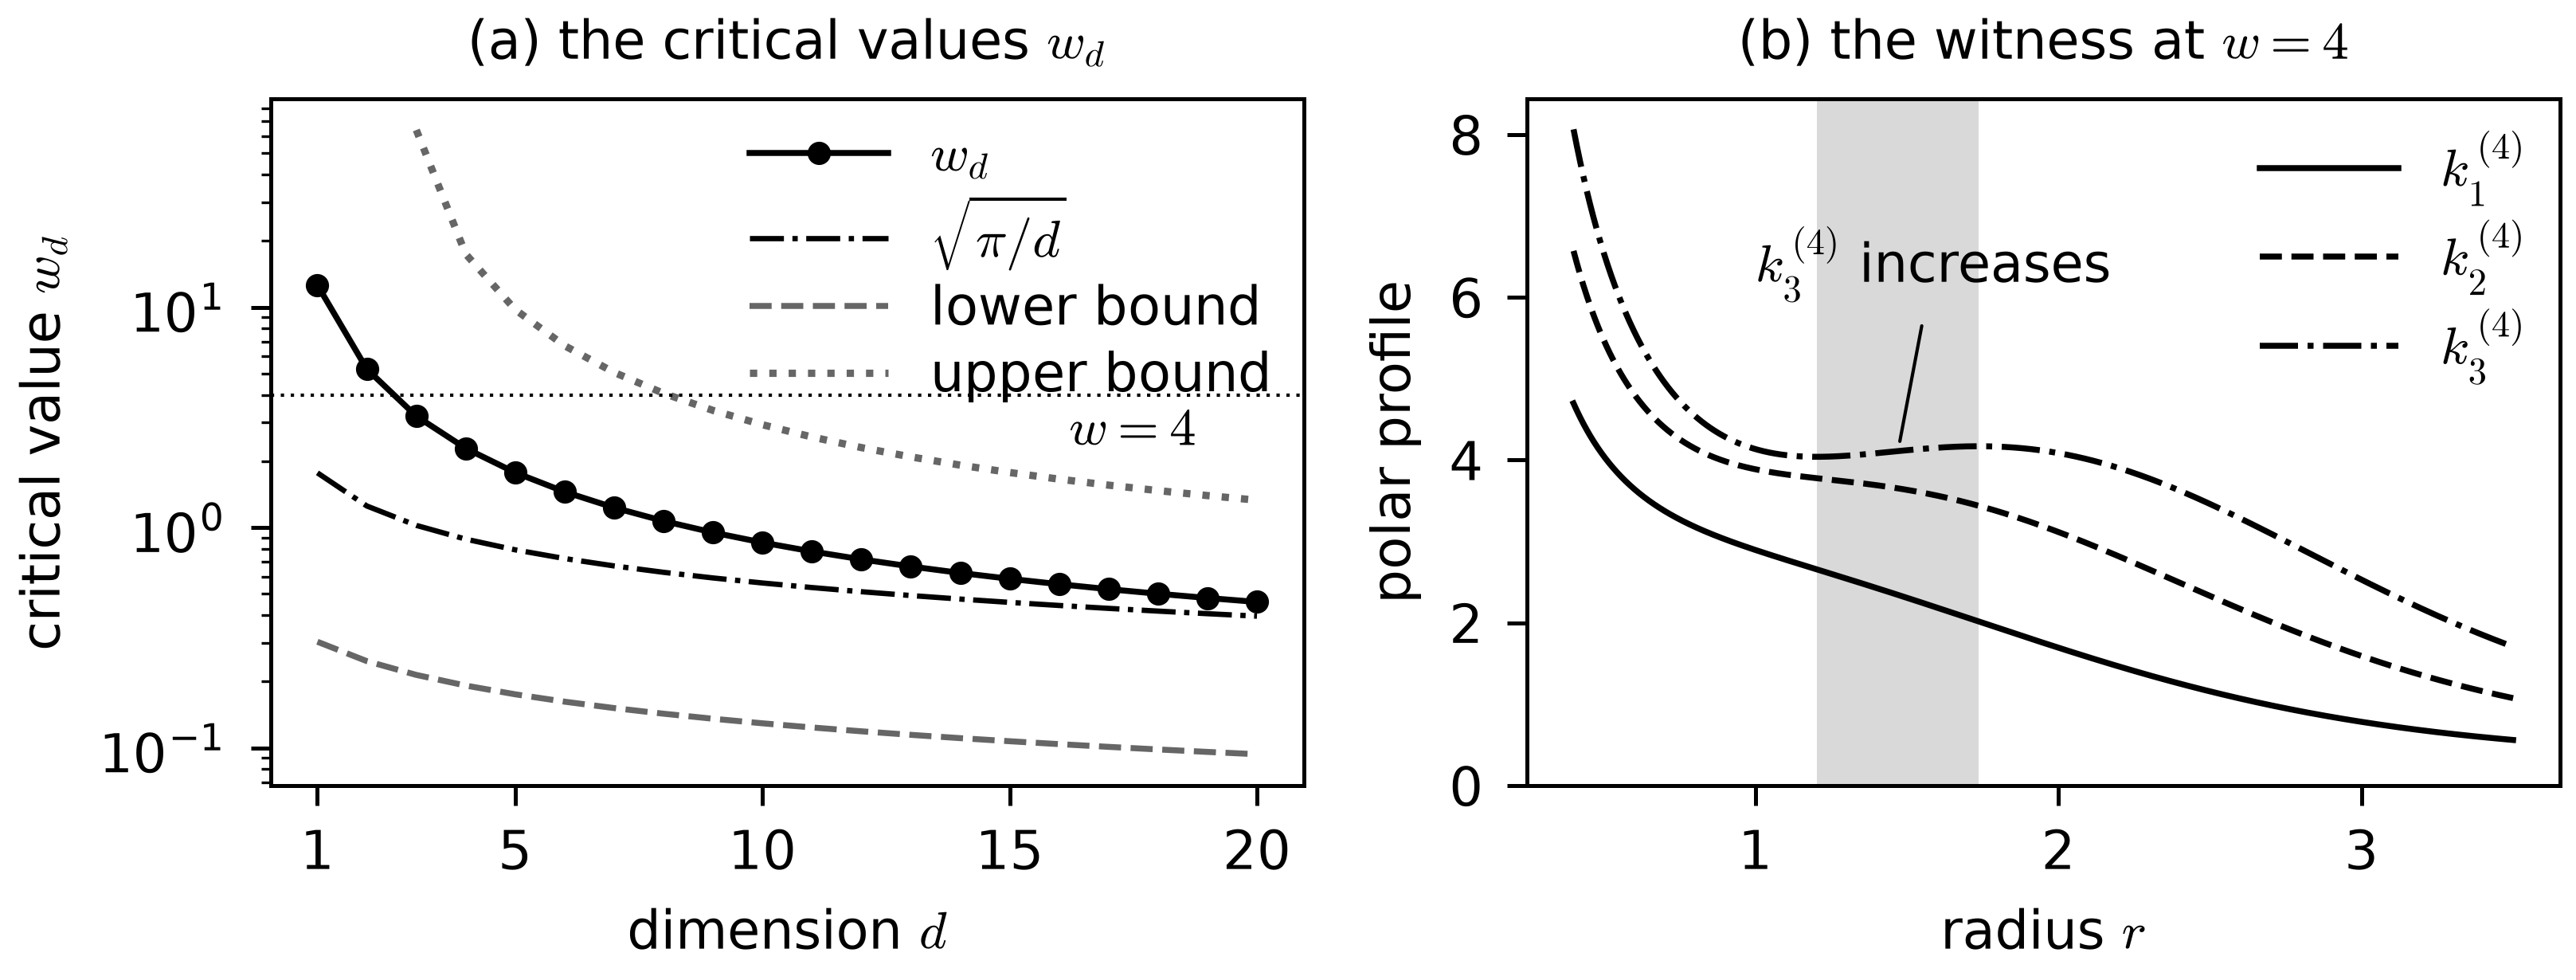
\includegraphics[width=0.86\textwidth]{fig-thresholds.png}
\caption{(a) The critical values $w_d$ of Definition~\ref{def:filtration-thresholds} for
$d = 1, \dots, 20$, computed numerically, on a logarithmic scale, with the lower and the upper
bound displayed in the text, the upper one for $d \ge 3$, and the asymptote $\sqrt{\pi/d}$ of
Theorem~\ref{thm:separating-family-critical-values}(3). The horizontal line $w = 4$ crosses the
sequence between $d = 2$ and $d = 3$. (b) The polar profiles $k^{(4)}_d$ of $F^{(4)}$
(Definition~\ref{def:filtration-thresholds}) in dimensions $1$, $2$ and $3$: nonincreasing in
dimensions $1$ and $2$, increasing on the marked interval, about $(1.20, 1.74)$, in dimension
$3$. Computed by a script deposited with the paper.}
\label{fig:thresholds}
\end{figure}

As laws the members of the family are ordinary kernels in every dimension. For every $w > 0$ and
every $D$ the function $e^{-F^{(w)}(|\xi|)}$ is the transform of a Gaussian variance mixture on
$\RR^D$, a rotation-invariant infinitely divisible law
(Proposition~\ref{prop:separating-family-mixtures}(2)). In the dimensions that do not admit
$F^{(w)}$ that law lacks self-decomposability alone, the property that gives a cascade its
stages (its clause (3)). So the family separates a kernel in every dimension from a cascade in
every dimension. Its delay profile is not monotone, and its delay exponent $F^{(w)}_{\mathrm I}$
is not causally admissible: otherwise $F^{(w)}$ would be a member of $\mathcal{S}$, and so of
every $\mathcal{A}_D$ (Proposition~\ref{prop:line-filtration}(2)).

\begin{remark}[relation to the line]\label{rem:isotropic-line}
At $d = 1$ the definitions, the classification and the threshold of this section are those of the
line. $\Orth(1) = \{\pm1\}$, so Definition~\ref{def:isotropic-operator-family} is
Definition~\ref{def:line-family}, Corollary~\ref{cor:isotropic-classification-operators} is
Theorem~\ref{thm:line-classification}, and $\mathcal{A}_1$ is the admissible cone. The polar
profile $k_1$ is the folded profile of \ref{eq:admissible-line}, so $k_1(0{+})$ is the constant
$c$ of Corollary~\ref{cor:line-threshold}, whose two regimes and threshold are
Theorem~\ref{thm:origin-boundedness-d}(2), (4) and (5). What of the line theory is not carried to
$\RR^d$ is said in \S\ref{sec:conclusion}.
\end{remark}

% §4 Conclusion, with the open problems as its subsection 4.1 (Q-0408; the file was
% 04-open-problems.tex and the section "Open problems") --- paper-only. Q-0307 (the split at §3 | §4, adr/0001): the single article's
% section 6 (paper/06-open-problems.tex), problem 4, "The origin in dimension d >= 2", moved here
% verbatim but for its \ref to the affine paper's section; its other problems are about the affine
% theory and stayed there. Stated as open, never promised (hub RELEASES.md rule 1); no statement of
% the paper depends on an answer.
%
% Q-0428 (the rewrite after the external review, round 1; records/affine/
% REPOSITIONING-paper-iso-round2.md). The conclusion is on the footing of section 1: what the
% hemigroup axioms give in dimension d, in the order of the three questions, and what follows for
% a family taken from the line to the plane or to space. The paragraph that listed what is new
% and what was not found stated is gone (the direction of the author of 2026-10-12). Each sentence
% restates a statement of section 3, compared with it (WRITING.md section 5): "from scale zero"
% and "no Gaussian part" for the threshold; c < d and c = d apart for the rate; the dictionary
% for the exponents of logarithmic growth, with its two conditions on the law; the jump test as
% Corollary cor:dictionary-filtration(1) states it. 4.1: the two questions that Q-0425 answered
% (the slowly varying factor through the polar profile; the limit of sqrt(d) w_d) are removed
% with their TODO(Q-0425). What remains: the derivatives at the centre for c > d, and the stages
% from a positive scale. (Whether a step witness stays infinitely divisible one dimension up was
% the third until Q-0448: Proposition prop:step-exponent-dimensions answers it.) No sentence says
% what a search of the literature found.
% Q-0428, the fixes round (records/affine/REPOSITIONING-paper-iso-round2-fixes.md): the practice paragraph
% reduced to what a user takes away, the limitations in section 4 proper, the open problems each
% specific.
% Q-0431 (the author's section review of 2026-10-12, records/affine/REVIEW-author-paper-iso.md).
% The opening leads with the main result in the terms of the contributions paragraph of section
% 1 (the kernels of the isotropic scale spaces are the rotation-invariant self-decomposable
% laws), and "The axioms of the line ... name no dimension" is gone: the author removed the same
% phrase from the abstract ("it is said that it is on the line"). The last sentence of the third
% paragraph says "taken alone" of a Cin ray, as section 3.4 now does: the exponents admitted in
% the plane are still superpositions of the rays and a Gaussian term.
\section{Conclusion}\label{sec:conclusion}

% Q-0448 (the author's decision of 2026-10-13: what is said twice goes; exposition item 4 of
% records/affine/reviews/VERIFY-round2-length-and-exposition.md). The answers are given once,
% in section 1. This section keeps the limitations and the open problems. The sentence on the
% main result says "from scale zero" (review B, R4: the stages are kernels of the family and
% are not self-decomposable in general).
The hemigroup axioms define, in every dimension, the scale spaces whose kernels from scale zero
are the dilations of a rotation-invariant self-decomposable law, and every such law other than
the point mass at the origin is such a kernel
(Corollary~\ref{cor:isotropic-scale-zero-kernels}). \S\ref{sec:introduction} says what follows for
the kernel at its centre and for the dimension.

% The limitations, in section 4 proper (the register review, flag 9). The generator on the line
% is the cone paper's Prop. 6.2.
% Q-0448, the blind draft review (flag 7): the limitations are listed here and nowhere else
% (the first paragraph of section 1 and its "Scope" had three of them). Of a stage the
% sentence says what Proposition prop:isotropic-stages gives, the point mass with its size, and
% what it leaves, the smoothing part at its centre, which is the open problem "The stages".
The paper has four limitations. It gives no generator of
the scale evolution: the evolution equation that the cone paper has on the line
\prog{B}{Prop.~6.2} is not carried to $\RR^d$. It proves nothing in $\RR^d$ on locality or on
the extrema of the smoothed signal. Its statements on the centre are about the kernels from
scale zero: of a stage $\mu_{s,t}$ with $s > 0$ and no Gaussian part it gives the point mass
and its size
(Proposition~\ref{prop:isotropic-stages}), and it does not examine the smoothing part at its
centre. And the dictionary covers the
exponents of logarithmic growth only: for the kernels
with a Gaussian part or with $c = \infty$ the paper matches no law on $\RR^d$ with the exponent.

\subsection{Open problems}\label{sec:open-problems}

% Each question names the regime and the quantity (the register review, flags 36 and 37); no
% count is announced (flag 38). What is not treated is in section 4, as limitations.
\paragraph{The derivatives.} Let $d + N - 1 < c < d + N$ with an integer $N \ge 1$. The density
then has $N - 1$ continuous derivatives (Theorem~\ref{thm:origin-boundedness-d}(2)), and the
theorem says nothing of the next one. Is the radial derivative of order $N$ of the density
asymptotic at the centre to a constant times $|x|^{c-d-N}$ times the slowly varying factor $K$
of Proposition~\ref{prop:origin-rate-profile-d}, as the density itself is for $c < d$? And what
takes the place of the logarithm at $c = d + N$? On the line both are answered by Sato and
Yamazato, for every finite $c$ (\sscite{sato1978distribution}, Thms.~1.6 and~1.7).

% Q-0448 (the second external round, review D, R1 and R2; VERIFY-round2-mathematics.md, items
% 12 and 13): the question which stages have a density and which a point mass is answered by
% Proposition prop:isotropic-stages, and what is left of it is asked here. The question on the
% step witnesses is answered by Proposition prop:step-exponent-dimensions and has left the list.
\paragraph{The stages.} Let the kernels have no Gaussian part. Is the absolutely continuous
part of a stage $\mu_{s,t}$ with $s > 0$ bounded near the centre when $c$ is finite
(Proposition~\ref{prop:isotropic-stages}(2)), and what number decides it? And is the density of
a stage bounded when $c = \infty$?
% Q-0450 (the scope audit of 2026-10-13, mismatch 5): with a Gaussian part the stage has a
% bounded smooth density (Proposition prop:isotropic-stages(3)(c)), so both questions, and the
% limitation above, are for the kernels with no Gaussian part.


% Appendix A (Q-0291): the proofs moved out of section 3, in its order; the main text names each
% and points here. Appendix B (Q-0414): the inventory of the formal verification that section 1.1
% names (WRITING.md section 4), under its own "trust base" markers.
\appendix
% Appendix A --- deferred proofs of section 3. Moved out of section 3 (Q-0291, the author's decision
% of 2026-10-04 to shorten sections 3 and 4 by moving material to appendices, as Q-0290 did for
% section 5; records/affine/move-sections-3-4-to-appendices*.py, three passes). The proofs are
% unchanged but for their headings, in main-text order: lem:radial-marginal,
% lem:isotropic-marginal-family, the sufficiency and uniqueness halves of
% thm:isotropic-classification, prop:isotropic-polar-reading, prop:isotropic-bridge (3.2);
% lem:positive-transform-origin, lem:isotropic-exponent-log, thm:origin-boundedness-d (3.3);
% lem:threshold-monotone, lem:threshold-limit, thm:filtration-strict, thm:no-cin-ray-in-the-plane
% (3.4). Every statement stays in section 3, which keeps the necessity half of
% thm:isotropic-classification: the reduction to the line.
%
% Q-0310 (the whole-paper review's notation flags; records/affine/
% REVIEW-paper-whole-fixes-paper-iso.md), in the proofs only: the contraction ratio of
% self-decomposability is lambda (it was c, which is the profile at the origin); the
% sphere-averaged profile is \bar k (K is the constant of lem:threshold-limit and the Bessel
% function); the unit vector of lem:isotropic-exponent-log's proof is \widehat\xi (theta is the
% Matern range); the shadow measure of thm:no-cin-ray-in-the-plane's proof is \bar\nu (m is
% (d+1)/2); "profile" is qualified. The gauge ratio c of the uniqueness proof matches the shared
% statement and is owed at the blueprint (records/affine/GATE-paper-iso.md).
%
% Q-0311 (the blind review records/affine/REVIEW-paper-iso.md, flag 3): the three proofs that were
% sketches (lem:isotropic-exponent-log, thm:origin-boundedness-d, lem:threshold-limit) are now the
% blueprint's proofs of record in full (blueprint/src/parts/03-isotropic.tex), transcribed with the
% paper's conventions: "Lemma~\ref" for a bare \ref, the cited facts by their paper names C1-C4,
% the unit vector \widehat\xi for the blueprint's theta (the Matern range), the radius r of the
% punctured balls in clause (3) for the blueprint's eta (the sphere variable), y for the dummy
% variable of clause (4), and C_k defined in clause (3), where the blueprint uses it for the delay
% profile's tail without a definition. No proof of the paper is a sketch now. The remark on
% 3/2 - sqrt 2 moved here from section 3.4, after its proof (flag 31).
%
% Q-0316 (pass 2, the blind register review REVIEW-register-paper-iso.md, Appendix A flags 1-25):
% the proof-zone flags were fixed at the blueprint's proofs of record, and every proof here is
% re-transcribed from them verbatim by records/affine/transcribe-proofs-q0316.py (the cited facts
% through \ledger, which macros.tex prints as C1-C5). Two proofs are new: those of
% prop:isotropic-radial-monotone and lem:delay-polar-profile (the witness's membership, flag 1).
% The remark after lem:threshold-monotone is paper prose (flag 22), shortened.
%
% Q-0328: the proof of record of prop:origin-lower-bound-d, verbatim (records/affine/
% transcribe-q0328-origin-lower-bound.py), after that of thm:origin-boundedness-d. Its register was
% brought to the Q-0316 pass's at the blueprint first (seven participial clauses and two semicolons
% made sentences, no step changed).
%
% Q-0406 (pass 6, the author's review of section 3; records/affine/REVIEW-author-paper-iso.md):
% A.1 is the proof of the one lemma on operators and kernels, in both directions, from the two
% proofs of record (the comment above it says how). Item 5 of the brief: a place of the line paper
% or the cone paper that section 2 restates is cited at the restatement, through \restated and
% \restatedp (macros.tex; the blueprint changed by the same markup, so the proofs stay verbatim);
% the proof of prop:isotropic-bridge drops a restatement that section 2 gives, and is pinned. Not
% touched: the proof of thm:filtration-strict, which Q-0381 is rewriting on another branch (its
% [B, Prop. 4.9(1)] and (4) are Proposition prop:line-filtration(1) and (3) and are owed).

% Q-0448 (the split into a paper and a supplement; the author's decision of 2026-10-13, option
% (b) of records/affine/reviews/VERIFY-round2-length-and-exposition.md, section 3): this file is
% Appendix A of the paper. It keeps the notation, the sources, the proofs of the classification,
% the statements that the main text names and that are proved in the supplement, and the
% statements that Lean did not check, with their proofs. The proofs that Lean checked are in
% supp-proofs.tex, each cut from this file unchanged (records/affine/split_q0448.py).
% `linkage check` reads every .tex file of the directory and matches a proof to its statement
% by the \ref of its heading, so a proof in the supplement is still compared with the blueprint.
% One rule decides the place of a proof: checked by Lean, the supplement; proved in print only,
% here. Two exceptions, both in print: the proofs of the classification (short, and the result
% the paper is about), and the proof of Proposition prop:profile-one-dimension-down (half a
% page, and the corollary proved in print reads it).
% A statement that changes status moves by one edit of the lists of section 1.1 and by moving
% its proof between this file and supp-proofs.tex.
\section{Notation, sources, and the proofs given in print}\label{app:isotropic-proofs}

This appendix has the notation (Table~\ref{tab:notation}), the sources of the statements
(\S\ref{sec:isotropic-sources}), the proofs of the classification
(\S\ref{app:classification-proofs}), five statements that the main text names and does not state
(\S\ref{app:further-statements}), and the proofs of the statements that are proved in print
only (\S\ref{app:print-proofs}). The proofs that Lean checked are in \suppl, except those of the
classification and that of Proposition~\ref{prop:profile-one-dimension-down}, which is in
\S\ref{app:print-proofs}.
% Q-0448, the blind draft review of the split (flag 4): the sentence that says how the numbers
% of the supplement read (\supplnumbers) is in "Plan of the paper", before the first S-number.

% Q-0428: the notation table of section 2.7, moved here as it stood (its rows for the new symbols were
% added in the same item).
% Q-0310: the notation table the brief asks for at the end of section 2 (review flag 25 and the clash
% map; records/affine/REVIEW-paper-whole-fixes-paper-iso.md). Paper-only; every row was checked
% against its first use. The second roles named are in shared statements and are owed at the
% blueprint (records/affine/GATE-paper-iso.md; Q-0311 added lambda_d, t and a, review flag 26).
% Q-0430: a longtable, as Table tab:in-print now is (sources.tex). As a float it could not stand
% on the appendix's first page and came out after that table, which is no float any more, so
% that Table 2 was printed before Table 1. Its rows and its caption are unchanged; N is the
% column p in the size of the table's text (main.tex).
{\renewcommand{\arraystretch}{0.88}
\begin{longtable}{@{}N{0.2\textwidth}N{0.76\textwidth}@{}}
\toprule
symbol & role \\
\midrule
\endhead
\bottomrule
\endfoot
\bottomrule
\addlinespace
\caption{Notation of \S\ref{sec:isotropic} and Appendix~\ref{app:isotropic-proofs}.}
\label{tab:notation}
\endlastfoot
$\xi$, $\omega$ & frequency on $\RR^d$, on the line \\
$s \le t$, $\chi$, $S_\lambda$ & scales; a gauge; the action of a dilation on the scales \\
$\lambda$, $\rho_\lambda$; $\lambda_d$ & a dilation factor; for $\lambda \in (0,1)$ in
  \ref{eq:self-decomposable}, the contraction ratio, and $\rho_\lambda$ the residual; the number
  $2^{-d/2}$ in Lemma~\ref{lem:threshold-monotone}, and the mean of $\log|\langle e,\eta\rangle|$
  over the sphere in Proposition~\ref{prop:isotropic-exponent-profile} (in C2, $\lambda$ is a
  measure on the sphere) \\
$\Phi_{s,t}$; $T_a$, $R_Q$, $D_\lambda$ & the operators of a family; on $L^1(\RR^d)$, the
  translation by $a$, the action of $Q \in \Orth(d)$ and the dilation by $\lambda$
  (Definition~\ref{def:isotropic-operator-family}; on the line $\tau_a$, $R$ and $D_\lambda$) \\
$\mu_{s,t}$; $\nu_{s,t}$, $\kappa_{s,t}$ & the kernels of a family on $\RR^d$; kernels on the line \\
$x$; $\mu^{\mathrm I}_{x,y}$ & a point of $\RR^d$ or of $\RR$; in $\mu^{\mathrm I}_{x,y}$, $x \le y$
  are scales of a time-causal family \\
$u_K$, $\Lambda$ & in C5, the uniform law on a convex set $K$, and the mixing measure \\
$F$, $F_d$, $F_{\mathrm I}$ & an exponent on the line \ref{eq:admissible-line}; the exponent of an
  isotropic origin datum on $\RR^d$; a causally admissible exponent \\
$a_{\mathrm V}$, $a$, $b_0$ & the Gaussian coefficient on the line; that of an isotropic origin datum,
  $a_{\mathrm V} = \tfrac12 a$ (in Lemma~\ref{lem:isotropic-exponent-log}(2), a dilation factor);
  the drift of a delay datum \\
$k$, $k_d$, $k_{\mathrm I}$ & the folded profile; the polar profile, the radial \Levy{} density times
  $|S^{d-1}|\,r^d$; the delay profile \\
$c$ & the profile at the origin, $k_d(0{+})$, and $k(0{+})$ on the line; in the uniqueness clause of
  Theorem~\ref{thm:isotropic-classification}, the ratio of two gauges \\
$\nu_d$, $f_d$; $p$, $q$ & the \Levy{} measure of an isotropic origin datum, and its radial
  density; the density of a kernel and its radial form, $p(x) = q(|x|)$ \\
$K$, $C_k$, $\varkappa_d$ & the slowly varying factor of the rate, the integral of the
  polar profile beyond radius $1$, and a constant of the dimension
  (Proposition~\ref{prop:isotropic-exponent-profile}); $K_\nu$ is a Bessel function, and in
  Lemma~\ref{lem:threshold-limit} $K$ is a number \\
$A$, $Q$, $B$; $R(d,c)$ & the constants of Proposition~\ref{prop:origin-rate-profile-d}, and that
  of Lemma~\ref{prop:origin-rate-d}. Elsewhere $A_\beta$ is the constant of
  Proposition~\ref{prop:origin-upper-bound-d}, $Q$ an orthogonal matrix
  (Definition~\ref{def:isotropic-operator-family}, Proposition~\ref{prop:radial-dictionary}), $B$
  a Borel set (Theorem~\ref{thm:origin-boundedness-d}(4) and C2), $R_Q$ the action of $Q$, and
  $R$ a random radius (Proposition~\ref{prop:radial-dictionary}) \\
$L$; $\mathcal{L}$ & the slowly varying factor of a transform, $\widehat\mu = |\xi|^{-c}L(|\xi|)$;
  the function $\int_s^1 K(y)\,dy/y$ of Proposition~\ref{prop:origin-rate-profile-d}(3) \\
$e$ & a unit vector of $\RR^d$, as in $\widehat\mu(e/s)$; in $e^{-C_k}$ and the like, the base of
  the exponential \\
$\Omega_d$, $\phi$, $X$ & in \S\ref{sec:isotropic-filtration}, the characteristic function of the
  uniform law on the unit sphere along a ray; that of a rotation-invariant random vector $X$
  (in \S\ref{sec:line-origin} $\phi_1$ is a density, and in
  Proposition~\ref{prop:isotropic-exponent-profile} $X$ is a real variable) \\
$\mathcal{A}_d$, $\mathcal{A}_\infty$, $\mathcal{S}$ & the classes of
  Proposition~\ref{prop:line-filtration}; their intersection; the subordinated slice \\
$b\,\Cin(\tau|\omega|)$; $\tau_a$ & a member of a $\Cin$ ray, of folded profile
  $b\,\mathbf{1}_{(0,\tau)}$; the translation by $a$ \\
$\gamma$, $\theta$; $\alpha$; $\vartheta$ & the \Matern{} index and range; the stable kernels, of
  index $2\alpha$; the shape of the Student-t kernels \\
$W$, $Z$; $T_1$ & a random delay and a standard normal vector; the scaled inverse-gamma delay \\
$w$, $w_d$, $M_d$, $m$ & the parameter of the separating family, its critical values,
  $m = (d+1)/2$ (Definition~\ref{def:filtration-thresholds}) \\
$\tau$ & the cut-off of a $\Cin$ ray and of a step datum; in \S\ref{sec:isotropic-sources},
  the time of a \Levy{} process, the kernel being its law at $\tau = 1$; a constant of
  Proposition~\ref{prop:origin-lower-bound-d} \\
$s$ & in Proposition~\ref{prop:origin-rate-profile-d} and in Lemma~\ref{prop:origin-rate-d} of
  \suppl, a distance from the centre of the kernel, not a scale \\
$g_t$, $g^{(d)}_u$ & the heat kernel at variance $t$ (here $t$ is not a scale); the centred
  Gaussian law of covariance $uI$ \\
\end{longtable}
}

% Q-0428, the fixes round: the one home of the attributions (sources.tex). It stands here and not
% at the end of section 3 because of the length.
% Sources --- the one home of the attributions of section 3 (Q-0428, the fixes round; the register
% review of sections 3.3 to 4, structural change 1, flags 1, 8, 16, 17, 18; the author's direction
% of 2026-10-12: attribution exact and made once). Paper-only: nothing here is shared with the
% blueprint. Until this round the table stood in the opening of section 3.3, before every
% statement it lists, with a third column that graded each statement ("restated", "extended",
% "proved"); the column is gone, and the cells are the source, its anchor and the case that the
% source covers. The statements of the body carry no sentence of attribution, but for two names a
% reader needs to use a statement (Watanabe after the shape; Halgreen for the Student-t clause).
%
% Anchors, each from the note that read it at the page (records/affine/), all confirmed by the
% citation audit of 2026-10-12 (CITATION-AUDIT-paper-iso-2026-10-12.md, 45 sites, all right):
% sato1999levy, Thm. 16.1, p. 99, by Sato 1991, p. 117, and the proof of Thm. 8.1(ii), p. 40
% (READING-sato1999levy-prior-art.md); hazod2001stable, Thm. 2.14.21, p. 383, with its limit
% condition (READING-hazod2001stable.md; the audit's note on row 38); knopova2013note, p. 126 and
% Lemma 2.6, p. 132 (READING-knopova2013note.md); grzywny2019asymptotic, Example 3, Thm. 3.5,
% Prop. 5.3, (5.4), by the numbers of the published article (READING-grzywny2019asymptotic.md);
% sato1978distribution, Lemma 5.1, p. 298, Thm. 1.7, p. 277 (READING-sato1978distribution.md);
% bingham1987regular, Thm. 3.7.3, pp. 162-163; watanabe1983isoperimetric, Proposition, p. 488
% (READING-watanabe1983isoperimetric.md: the law at each time of a symmetric Levy process whose
% Levy measure is isotropic unimodal; the audit's note on row 39); leonenko2013tauberian, Thms. 3
% and 4, arXiv v1 (READING-leonenko2013tauberian.md, with its addendum: the survey is where the
% theorems are collected; the citation is to the book); bingham1997abel, Thms. 1.1 and 1.2 and
% (1.4) of the preprint (READING-bingham1997abel.md, with its addendum: both for a function
% ultimately decreasing to zero); cygan2017asymptotic,
% Thms. 8 and 9, arXiv v2 (READING-cygan2017asymptotic.md); jurek1983integral, Thm. 3.2, p. 252,
% Thm. 4.1, p. 254, Thm. 7.2, p. 259 (READING-jurek1983integral-driving-process.md);
% sato1984operator, Thm. 4.1, p. 86; jurek1992operator, Cor. 1.7, pp. 1056-1057;
% jurek1993operator, Prop. 3.9.6, pp. 180-182; schoenberg1938metric, section 2.1 and Thm. 2,
% pp. 816-817; gneiting1999radial, p. 94; cambanis1981theory, Lemma 2, p. 371, Cor. 2, p. 372
% (the radius of a projection); fang1990symmetric, Thm. 2.10, p. 36 (the density of the
% projection itself, the audit's note on row 17; never its remark of p. 37); the cone paper,
% Lem. 4.12 and Rem. 4.10; trabs2014infinitely, Prop. 1, p. 58.
%
% Q-0430 (the primary sources, read at the page images; records/affine/
% CITATIONS-primary-sources-A.md and -B.md with their reading notes, and
% CITATION-CHANGES-q0430.md for every citation added, changed or left out, with the reason):
% leonenko1999limit, Thm. 1.4.3, p. 65 (the implication from the covariance function to the
% spectral function: 0 < alpha < n, n >= 1, no monotonicity), its proof on p. 104 from
% Lemma 1.4.11, p. 72; Thm. 1.4.4, pp. 66-67 (the book prints the monotonicity of the density
% as "decreasing for ||lambda|| >= k", the survey has (0, eps]: the cell says "a nonincreasing
% function of the radius" and quotes neither; nor the book's remark on c_5(1, alpha), p. 67,
% nor the constant of its Example 1.4.1, both misprinted); the credits of its Comments, p. 351;
% leonenko1991tauberian, Corollary of Lemma 2, p. 1542 of the translation (a pure power, the
% constant L(n) a_n(alpha)/Gamma(1 + alpha) with L(n) "a constant");
% soni1975slowlya, Thms. 1 and 2, p. 169, with the remark of p. 171; soni1975slowlyc,
% Thms. 17(a) and 18(a), pp. 613-614, the Hankel kernel on pp. 617-618 (its display of the
% coefficients c_j is off by a factor sqrt 2: no constant is taken from it). Bingham 1972 and
% Ridenhour and Soni 1974, to which Bingham and Inoue give their Theorem 1.2, are not cited:
% the first is a theorem for another transform, the second the converse implication under
% other conditions (READING-bingham1972tauberian.md, READING-ridenhour1974parseval.md).
% sato1983stationary, Thms. 5.1-5.3, pp. 546-547; jurek1982integral, Thms. 2.1 and 3.1,
% folios 388 and 390; wolfe1982continuous, Thm. 1, p. 306, Cor. 3, p. 307;
% daley2014dimension, Prop. 11 with (3.8), p. 1821, Lemma 12, p. 1822 (its Thm. 4, p. 1815, was
% read in the text layer only and is not cited).
% The versions cited (the author, 2026-10-12: the copies held are the ones the paper cites):
% cygan2017asymptotic and leonenko2013tauberian in the numbering of their arXiv versions (v2,
% v1), bingham1997abel in that of the Hokkaido preprint (no. 370), said once, in the caption.
% Their published numbering was not compared. grzywny2019asymptotic is cited by the statement
% numbers of the published article and never by a page.
%
% Q-0450 (the citation audit of 2026-10-13, CITATION-AUDIT-paper-iso-2026-10-13.md, 54 sites):
% two rows corrected. bogdan2014density, (19): p. 11 of the arXiv version held (v2), not p. 9,
% which has (17) and (18); read again at the page for this item. watanabe1983isoperimetric,
% Proposition, p. 488: its condition (3) is S = aI with a >= 0 and the Levy measure isotropic
% unimodal, so the row and the sentence after Proposition prop:isotropic-radial-monotone name
% the Gaussian covariance as well.

\subsection{Sources}\label{sec:isotropic-sources}

Table~\ref{tab:in-print} says where the main statements of \S\ref{sec:isotropic} are in print,
statement by statement, with the case that each source covers. Several of the sources are
written for a \Levy{} process (\S\ref{sec:line-bridge}): with a
law of exponent $F_d$ they study the laws with the transforms $e^{-\tau F_d}$, $\tau > 0$, the
laws of the process at the times $\tau$. The time is not the scale of this paper. The time
multiplies the exponent, and the scale rescales the frequency. A kernel is the law at time $1$,
and the law at time $\tau$ is a kernel with $\tau c$ in place of $c$.

% Q-0430: a longtable (it is longer than a page and breaks between rows). The struts of a row
% are those of the table's text size: \arraystretch is the ratio of the two line spacings.
{\renewcommand{\arraystretch}{0.81}
\begin{longtable}{@{}S{0.2\textwidth}S{0.76\textwidth}@{}}
\toprule
statement & where it is in print, and for which case \\
\midrule
\endhead
\bottomrule
\endfoot
\bottomrule
\addlinespace
\caption{Where the main statements of \S\ref{sec:isotropic} are in print, and for which case.
Three sources are cited in the numbering of the version that was read, which is not the
journal's: the Hokkaido preprint for \sscite{bingham1997abel}, and the arXiv versions for
\sscite{cygan2017asymptotic} and \sscite{leonenko2013tauberian}. The numbers of
\sscite{grzywny2019asymptotic} are those of the published article, and the pages of
\sscite{leonenko1991tauberian} those of the English translation.}
\label{tab:in-print}
\endlastfoot
Thm.~\ref{thm:isotropic-classification} and Cor.~\ref{cor:isotropic-scale-zero-kernels}, the
classification &
  Read on laws: a process with independent increments on $\RR^d$ that is self-similar up to a
  change of scale and a deterministic shift has self-decomposable laws, and every
  self-decomposable law but a point mass is the law at time $1$ of one
  (\sscite{sato1999levy}, Thm.~16.1, p.~99, due to Sato \sscite{sato1991selfsimilar}). On
  groups, a law is self-decomposable exactly when it is the limit of the kernels $\mu_{0,t}$ of
  a continuous hemigroup that a contracting one-parameter group of automorphisms maps into
  itself (\sscite{hazod2001stable}, Thm.~2.14.21, p.~383). \\
\addlinespace
Thm.~\ref{thm:origin-boundedness-d}, the threshold &
  On the line: \S\ref{sec:line-origin}. For the laws of a \Levy{} process on $\RR^d$: bounded
  when $c > d$, unbounded when $c \le d/2$ (\sscite{knopova2013note}, p.~126, and the proof of
  Lemma~2.6, p.~132). The threshold with its boundary case $c = d$, for two families: the
  \Matern{} kernels (the sources quoted in Example~\ref{ex:matern}, where two of the kernels
  above the threshold are given with their derivatives) and the laws with transform
  $(1 + |\xi|^\alpha)^{-\tau}$ (\sscite{grzywny2019asymptotic}, Example~3). \\
\addlinespace
Cor.~\ref{cor:origin-profile-exponent}, $c$ read off the exponent &
  Clause (1), for every infinitely divisible law: \sscite{sato1999levy}, proof of Thm.~8.1(ii),
  p.~40. Clause (2) for a finite $c$: on the line, an asymptotic form of the transform with its
  constant (\sscite{sato1978distribution}, Lemma~5.1, p.~298); in $\RR^d$ it follows from an
  equivalence for the \Levy{} processes whose laws are rotation invariant with radially
  nonincreasing densities (\sscite{grzywny2019asymptotic}, Thm.~3.5) by de Haan's theorem on
  functions whose increments are governed by a slowly varying function
  (\sscite{bingham1987regular}, Thm.~3.7.3, pp.~162--163). \\
\addlinespace
Prop.~\ref{prop:isotropic-radial-monotone}, the shape &
  For the law at each time of a symmetric \Levy{} process whose Gaussian covariance is a
  multiple of the identity and whose \Levy{} measure has a radially
  nonincreasing density: \sscite{watanabe1983isoperimetric}, Proposition, p.~488. That a
  self-decomposable law on $\RR^d$ which is not degenerate is absolutely continuous:
  \sscite{sato1999levy}, Thm.~27.13, p.~181, proved by Sato in 1982 (p.~196). \\
\addlinespace
Lemma~\ref{prop:origin-rate-d} of \suppl, the rate through the transform: clause (1) for
$c < d$, quoted before Proposition~\ref{prop:origin-rate-profile-d}, and clause (2) for $c = d$ &
  Clause (1), for a rotation-invariant probability law on $\RR^d$, $d \ge 1$, whose transform is
  $|\xi|^{-c}$ times a slowly varying factor, $0 < c < d$: the mass of a ball
  (\sscite{leonenko1999limit}, Thm.~1.4.3, p.~65, where the law is the spectral measure of a
  random field and the transform its covariance function), and the density when it is a
  nonincreasing function of the radius (the same book, Thm.~1.4.4, pp.~66--67). The book
  gives the two theorems for a transform asymptotic to a power to Leonenko and Olenko, and
  their proofs with a slowly varying factor to Olenko (p.~351). For a power the mass of a
  ball is \sscite{leonenko1991tauberian}, Corollary, p.~1542, with a constant that is not given
  in closed form. The survey \sscite{leonenko2013tauberian} collects both theorems, as its
  Thms.~3 and~4, with related ones. \\
\addlinespace
Lemma~\ref{prop:origin-rate-d}, through Hankel transforms &
  For $c > (d-3)/2$ the mass of a ball in clause (1) also follows from
  the Abel--Tauber theorem for Hankel transforms, in the direction from a function that is
  ultimately decreasing to zero to its transform. For a bounded function, which is the case
  $d \ge 3$: \sscite{soni1975slowlya}, Thm.~1, p.~169, with the remark on p.~171, and, as an
  equivalence for a function decreasing on the half-line, \sscite{soni1975slowlyc},
  Thm.~17(a), p.~613, with pp.~617--618 for the Hankel kernel. With local integrability in
  place of boundedness, and so for every $d$: \sscite{bingham1997abel}, Thm.~1.2. The mass of
  a ball in clause (2) follows from the boundary case of that theorem
  (\sscite{soni1975slowlya}, Thm.~2, p.~169, and \sscite{soni1975slowlyc}, Thm.~18(a),
  pp.~613--614, for a bounded function; \sscite{bingham1997abel}, Thm.~1.1 with (1.4)). \\
\addlinespace
Lemma~\ref{prop:origin-rate-d}, on the line, and the method of its proof &
  On the line: the theorem of Sato and Yamazato quoted in \S\ref{sec:line-origin}. The method
  of proof, an average of the transform against a positive kernel read as a Laplace transform of
  the mass of balls: with the Poisson kernel, for the spectral measure of a random field,
  \sscite{leonenko1999limit}, Lemma~1.4.11, p.~72, and the proof on p.~104; with the Gaussian
  kernel, in $\RR^d$, for the measure of the expected time that a \Levy{} process spends in a
  set, \sscite{cygan2017asymptotic}, Thm.~8 with its proof, and Thm.~9. The constant of the
  mass of a ball in clause (1), $R(d,c)\,|S^{d-1}|/c$, is the constant of these two theorems at
  the index $c$. \\
\addlinespace
Prop.~\ref{prop:origin-rate-profile-d}, the rate through the profile &
  On the line: the same theorem of Sato and Yamazato, with their lemma cited at
  Corollary~\ref{cor:origin-profile-exponent} above. In $\RR^d$, for the \Levy{} processes whose
  laws have radially nonincreasing densities and as the time $\tau$ tends to $0$: the density at
  $x$ is asymptotic to $\tau$ times the \Levy{} density at $x$ times the transform of the law at
  the frequencies of length $1/|x|$ (\sscite{grzywny2019asymptotic}, Thm.~3.9). The constant
  $R(d,\tau c)$ of the proposition for the law at time $\tau$ agrees with it in that limit. \\
\addlinespace
Props.~\ref{prop:origin-lower-bound-d} and~\ref{prop:origin-upper-bound-d}, the two bounds;
Lemma~\ref{lem:isotropic-exponent-log} &
  For the \Levy{} processes whose laws have radially nonincreasing densities, a lower bound and the
  comparison of a radially nonincreasing density with its average, on which the upper bound rests
  (\sscite{grzywny2019asymptotic}, Prop.~5.3 and (5.4)). The lemma on the line:
  \sscite{trabs2014infinitely}, Prop.~1, p.~58, and the same lemma of Sato and Yamazato. The
  two-sided estimates of \sscite{bogdan2014density} for such processes assume an exponent whose
  growth lies between two powers of positive order ((19), p.~11, of the arXiv version), which a
  finite $c$ excludes. \\
\addlinespace
Prop.~\ref{prop:isotropic-stages}, the stages &
  On the line, for the \Matern{} kernel of index $1$: the stage between two scales of ratio $r$
  as a mixture in which no displacement has the weight $r^2$ (\prog{B}{Prop.~7.2}, with (7.2)). \\
\addlinespace
Prop.~\ref{prop:radial-dictionary}, the dictionary &
  Clauses (1) and (2) are a case of the representation of a self-decomposable law as the limit
  law of the integrals $\int_0^t e^{-s}\,dY(s)$ of a \Levy{} process $Y$
  (\sscite{jurek1983integral}, Thms.~3.2 and~4.1, pp.~252 and~254; \sscite{sato1984operator},
  Thm.~4.1, p.~86): the case in which $Y$ moves by isolated jumps, at the rate $c$ and with the
  law of $X$. The representation is also in \sscite{sato1983stationary}, Thms.~5.1--5.3,
  pp.~546--547 (the law of a stationary process of Ornstein--Uhlenbeck type), in
  \sscite{jurek1982integral}, Thms.~2.1 and~3.1, pp.~388 and~390 (operator-self-decomposable
  laws on a Banach space), and, on the line, in \sscite{wolfe1982continuous}, Thm.~1, p.~306,
  and Cor.~3, p.~307 (the limit in law of $e^{-\gamma t}\int_0^t e^{\gamma u}\,dB(u)$,
  $\gamma > 0$). In radial form: \sscite{jurek1992operator}, Cor.~1.7, pp.~1056--1057, restated as
  \sscite{jurek1993operator}, Prop.~3.9.6, pp.~180--182. The classes of the radial
  characteristic functions on $\RR^m$ decrease in $m$, with the mixtures of Gaussians as their
  intersection (\sscite{schoenberg1938metric}, \S2.1 and Thm.~2, pp.~816--817), and strictly
  (\sscite{gneiting1999radial}, p.~94). \\
\addlinespace
Prop.~\ref{prop:profile-one-dimension-down} and Cor.~\ref{cor:dictionary-filtration}, the test
on the \Levy{} measure &
  For probability laws, the radius of a projection of a rotation-invariant law
  (\sscite{cambanis1981theory}, Lemma~2, p.~371, and Cor.~2, p.~372) and the density of the
  projection (\sscite{fang1990symmetric}, Thm.~2.10, p.~36). See also
  \sscite{daley2014dimension}: Prop.~11 with (3.8), p.~1821, for the radius law of a radial
  characteristic function in a lower dimension, the law of its radius times an independent
  variable with values in $(0,1)$. The formula of Lemma~\ref{lem:shadow-polar-profile} is (3.8)
  with the \Levy{} measure in place of the law. And Lemma~12, p.~1822: $\Omega_d$ is a
  characteristic function on $\RR^d$ and not on $\RR^{d+1}$, which is the last assertion of
  Corollary~\ref{cor:dictionary-filtration}(2). The representation of a
  self-decomposable law of which the $\Cin$ rays are the elementary terms on the line:
  \sscite{jurek1983integral}, Thm.~7.2, p.~259. \\
\addlinespace
Thm.~\ref{thm:separating-family-critical-values}, the separating family &
  The family, the members $w = 8$ and $w = 4$ as witnesses in dimensions $1$ and $2$, and the
  first critical values, computed numerically: \prog{B}{Lem.~4.12 and Rem.~4.10}. \\
\end{longtable}
}


\subsection{The proofs of the classification}\label{app:classification-proofs}

The necessity half of Theorem~\ref{thm:isotropic-classification} is proved in
\S\ref{sec:isotropic-reduction}. This subsection has the other proofs of the classification:
those of Lemma~\ref{lem:radial-marginal}, of the sufficiency and uniqueness halves of the
theorem, of Corollary~\ref{cor:isotropic-classification-operators}, of
Lemma~\ref{lem:isotropic-realisation}, of Proposition~\ref{prop:isotropic-polar-reading} and of
Corollary~\ref{cor:isotropic-scale-zero-kernels}.
The proofs of Lemmas~\ref{lem:operators-to-kernels} and~\ref{lem:isotropic-marginal-family},
which carry arguments of the line paper from the line to $\RR^d$, are in \suppl.

\begin{proof}[Proof of Lemma~\ref{lem:radial-marginal}]
\emph{(1).} $\pi_*\mu$ is a probability measure because $\pi$ is measurable, and for $\omega \in \RR$
\[
  \widehat\kappa(\omega) = \int_{\RR} e^{i\omega y}\,\kappa(dy)
   = \int e^{i\omega\langle e, x\rangle}\,\mu(dx) = \widehat\mu(\omega e) .
\]
A rotation-invariant law has a radial transform: if $|\eta| = |\eta'|$, let $Q$ be the identity when
$\eta = \eta'$ and otherwise the reflection in the hyperplane orthogonal to $\eta - \eta'$, an
element of $\Orth(d)$ with $Q^{\tp} = Q$ and $Q\eta = \eta'$; then
$\widehat\mu(\eta) = \widehat{Q_*\mu}(\eta) = \widehat\mu(Q^{\tp}\eta) = \widehat\mu(\eta')$.
Since $|\,|\xi|e\,| = |\xi|$, this gives $\widehat\mu(\xi) = \widehat\mu(|\xi|e) =
\widehat\kappa(|\xi|)$ for every $\xi \in \RR^d$. Since $-I \in \Orth(d)$ and $\pi(-x) = -\pi(x)$,
the image of $\kappa$ under $\omega \mapsto -\omega$ is $\pi_*((-I)_*\mu) = \kappa$, so $\kappa$ is
symmetric and $\widehat\kappa$ is real; hence so is $\widehat\mu$. For another unit vector $e'$ with
marginal $\kappa'$, $|\omega e'| = |\omega e|$ gives $\widehat{\kappa'}(\omega) = \widehat\mu(\omega e')
= \widehat\mu(\omega e) = \widehat\kappa(\omega)$ for every $\omega \in \RR$, so $\kappa' = \kappa$
by uniqueness of the transform on $\RR$.

\emph{(2).} If $\mu = \delta_0$ then $\pi_*\mu = \delta_0$. Conversely, if $\kappa = \delta_0$ then
$\widehat\kappa \equiv 1$, so $\widehat\mu \equiv 1 = \widehat{\delta_0}$ by (1), and
$\mu = \delta_0$ by uniqueness of the transform on $\RR^d$.

\emph{(3).} $\mu * \mu'$ is the image of $\mu \otimes \mu'$ under $(x,y) \mapsto x + y$, and
$\pi(x+y) = \pi(x) + \pi(y)$, so $\pi_*(\mu * \mu')$ is the image of $\pi_*\mu \otimes \pi_*\mu'$
under addition on $\RR$, which is $\pi_*\mu * \pi_*\mu'$. The other two identities are
$\pi(\lambda x) = \lambda\pi(x)$ and $\pi(0) = 0$.
\end{proof}

\begin{proof}[Proof of Theorem~\ref{thm:isotropic-classification}, sufficiency and uniqueness]
\emph{Sufficiency.} Let $\chi$ be a gauge and $F \in \mathcal{A}_d$ with $F \not\equiv 0$, and let
$(\mu_{s,t})$ be a family of probability measures on $\RR^d$ satisfying
\ref{eq:isotropic-classification}. First, $F$ is
continuous on $[0,\infty)$ with $F(0) = 0$: on $0 \le r \le \Omega$ the integrand of
\ref{eq:admissible-line} is at most $\max\{2,\Omega^2/2\}\,(1 \wedge x^2)\,k(x)/x$, which is
integrable by the two conditions on $k$, so dominated convergence applies. The axioms are read off
the transform, a probability measure on $\RR^d$ being determined by its
transform. (I1): the exponents of $\mu_{s,t}$ and $\mu_{r,s}$ add up to that of $\mu_{r,t}$, and
the exponent of $\mu_{t,t}$ is $0$. (I2): $F$ is continuous, and so is $\chi$, an increasing
bijection of $[0,\infty)$. (I3): $\widehat{Q_*\mu_{s,t}}(\xi) = \widehat\mu_{s,t}(Q^{\tp}\xi)$ and
$|Q^{\tp}\xi| = |\xi|$. (I4): with $S_\lambda := \chi^{-1}(\lambda\,\chi(\cdot))$, an increasing
bijection of $[0,\infty)$,
$\widehat{(\lambda I)_*\mu_{s,t}}(\xi) = \widehat\mu_{s,t}(\lambda\xi)
= \widehat\mu_{S_\lambda s,S_\lambda t}(\xi)$. (ND): let $s < t$ and suppose
$\mu_{s,t} = \delta_0$, so that $F(\chi(t)r) = F(\chi(s)r)$ for every $r \ge 0$. If $s = 0$ this
says $F(\chi(t)r) = 0$ for every $r$, and $\chi(t) > 0$ gives $F \equiv 0$. If $s > 0$ it says
$F(r) = F(\varkappa r)$ for every $r$, with $\varkappa := \chi(s)/\chi(t) \in (0,1)$. Iterating,
$F(r) = F(\varkappa^nr) \to F(0) = 0$, so again $F \equiv 0$ (\restated{V}{Lem.~6.3}{sec:line-facts}). Both contradict
$F \not\equiv 0$.

\emph{Uniqueness.} Let $(\chi',F')$ also satisfy \ref{eq:isotropic-classification}. Both exponents
are real, so taking logarithms of the kernels from scale zero, $F(\chi(t)r) = F'(\chi'(t)r)$ for
all $t, r \ge 0$, since $\chi(0) = \chi'(0) = 0$ and $F(0) = F'(0) = 0$. At $t' := \chi'^{-1}(1)$ this reads $F'(r) = F(c^{-1}r)$ with
$c^{-1} := \chi(t') > 0$. Hence $F(\chi(t)r) = F(c^{-1}\chi'(t)r)$ for all $t$ and $r$. If
$\chi(t) \ne c^{-1}\chi'(t)$ for some $t > 0$, then $F(r) = F(\varkappa r)$ for every $r$ with
$\varkappa := c^{-1}\chi'(t)/\chi(t) \ne 1$, and $F \equiv 0$ as in the previous paragraph (with
$\varkappa^{-1}$ in place of $\varkappa$ if $\varkappa > 1$), a contradiction. So
$\chi' = c\,\chi$. When $\chi(1) = \chi'(1) = 1$ this gives $c = 1$.
\end{proof}

% Q-0414, round 2: the proof of Corollary cor:isotropic-classification-operators, moved here
% from section 3.2 (records/affine/edits_q0414_round2_moves.py); the body is unchanged.
\begin{proof}[Proof of Corollary~\ref{cor:isotropic-classification-operators}]
\emph{Necessity.} Let $(\Phi_{s,t})$ be an isotropic cascade measurement family in dimension $d$.
By Lemma~\ref{lem:operators-to-kernels}(1) each $\Phi_{s,t}$ is convolution by a probability measure
$\mu_{s,t}$ on $\RR^d$, and by Lemma~\ref{lem:operators-to-kernels}(3) the family $(\mu_{s,t})$ is an
isotropic cascade family in dimension $d$. The necessity direction of
Theorem~\ref{thm:isotropic-classification} gives a gauge $\chi$ and an $F \in \mathcal{A}_d$ with
$F \not\equiv 0$ satisfying \ref{eq:isotropic-classification}.

\emph{Sufficiency.} Let $\chi$, $F$ and $(\mu_{s,t})$ be as in the statement. By the sufficiency
direction of Theorem~\ref{thm:isotropic-classification} the family $(\mu_{s,t})$ is an isotropic cascade
family in dimension $d$. By Lemma~\ref{lem:operators-to-kernels}(4) the operators
$f \mapsto \mu_{s,t} * f$, which are the $\Phi_{s,t}$, form an isotropic cascade measurement family
in dimension $d$.

\emph{Uniqueness.} Let $\chi'$, $F'$ and $(\mu'_{s,t})$ be as in the last sentence of the
statement. For $0 \le s \le t$ the probability measures $\mu_{s,t}$ and $\mu'_{s,t}$ give the same
operator $\Phi_{s,t}$, so they are equal, by the uniqueness clause of
Lemma~\ref{lem:operators-to-kernels}(1). Hence $(\chi', F')$ satisfies
\ref{eq:isotropic-classification} for the family $(\mu_{s,t})$, and the uniqueness clause of
Theorem~\ref{thm:isotropic-classification} gives $c$.
\end{proof}

\begin{proof}[Proof of Lemma~\ref{lem:isotropic-realisation}]
Let $\mu$ be a self-decomposable probability measure on $\RR^d$ with
$\widehat\mu(\xi) = e^{-F(|\xi|)}$, which the definition of $\mathcal{A}_d$ provides. For
$c \in (0,1)$ let $\rho_c$ be a residual of $\mu$. As $\widehat\mu(c\,\xi) = e^{-F(c|\xi|)} \ne 0$,
\ref{eq:self-decomposable} forces $\widehat\rho_c(\xi) = e^{-(F(|\xi|) - F(c|\xi|))}$; put
$\rho_0 := \mu$ and $\rho_1 := \delta_0$, so that this formula holds for every $c \in [0,1]$, as
$F(0) = 0$. For $0 \le s \le t$ put
\[
  \mu_{s,t} := \bigl(\chi(t)I\bigr)_*\,\rho_{\chi(s)/\chi(t)} ,
\]
with $\chi(s)/\chi(t) := 0$ when $\chi(t) = 0$, that is, when $s = t = 0$; then $\mu_{0,0}$ is
the image of $\mu$ under the zero map, $\delta_0$. Since
$0 \le \chi(s) \le \chi(t)$, the index lies in $[0,1]$, and
\[
  \widehat\mu_{s,t}(\xi) = \widehat\rho_{\chi(s)/\chi(t)}\bigl(\chi(t)\xi\bigr)
  = \exp\bigl[-\bigl(F(\chi(t)|\xi|) - F(\chi(s)|\xi|)\bigr)\bigr] ,
\]
because $\chi(s)/\chi(t)\cdot\chi(t)|\xi| = \chi(s)|\xi|$, both sides being $0$ when
$\chi(t) = 0$. Each $\mu_{s,t}$ is a probability measure, the image of one, so by the sufficiency
direction of Theorem~\ref{thm:isotropic-classification} $(\mu_{s,t})$ is an isotropic cascade family, and
it satisfies \ref{eq:isotropic-classification} with $(\chi, F)$ by construction.
\end{proof}

% Q-0414, round 2: Lemma lem:polar-decomposition, moved here from section 3.2 with its proof
% (records/affine/edits_q0414_round2_moves.py). The lead sentence is paper prose.
The proofs of this paper integrate against the \Levy{} measure of an isotropic origin datum in
polar coordinates. The identity \ref{eq:polar-decomposition} of
Definition~\ref{def:isotropic-origin-datum} is stated once, as a lemma.

% shared with blueprint lem:polar-decomposition
\begin{lemma}[the polar decomposition of an isotropic origin datum's \Levy{} measure]\label{lem:polar-decomposition}
Let $d \ge 1$ and let $(a, k_d)$ be an isotropic origin datum in dimension $d$ with \Levy{} measure
$\nu_d$. Then \ref{eq:polar-decomposition} holds for every nonnegative Borel $g$ on $\RR^d$
vanishing at the origin, $\sigma_{d-1}$ being the surface measure of $S^{d-1}$ and $|S^{d-1}|$ its
surface area.
\end{lemma}

\begin{proof}
By definition $\nu_d$ has the density $f_d(|x|) = k_d(|x|)(|S^{d-1}||x|^d)^{-1}$ on
$\RR^d \setminus \{0\}$. In polar coordinates $x = r\eta$, $dx = r^{d-1}dr\,\sigma_{d-1}(d\eta)$, so
for $g \ge 0$ Borel and vanishing at the origin
$\int g\,d\nu_d = \int_{S^{d-1}}\sigma_{d-1}(d\eta)\int_0^\infty g(r\eta)\,
k_d(r)(|S^{d-1}|r^d)^{-1}r^{d-1}\,dr$, which is \ref{eq:polar-decomposition}.
\end{proof}

\begin{proof}[Proof of Proposition~\ref{prop:isotropic-polar-reading}]
\emph{(1), forward.} Let $\mu$ be self-decomposable on $\RR^d$ with
$\widehat\mu(\xi) = e^{-F(|\xi|)}$. By \ledger{A4} it is infinitely divisible, and by \ledger{A3}(i)
it has a generating triplet $(A,\nu,\gamma)$. For $Q \in \Orth(d)$,
$\widehat{Q_*\mu}(\xi) = \widehat\mu(Q^{\tp}\xi) = \widehat\mu(\xi)$, so $Q_*\mu = \mu$. The
unit ball is $Q$-invariant, so substituting $x = Q^{\tp}y$ in the representation shows that
$Q_*\mu$ has triplet $(QAQ^{\tp}, Q_*\nu, Q\gamma)$. By uniqueness, \ledger{A3}(ii),
$QAQ^{\tp} = A$ and $Q_*\nu = \nu$ for every $Q$. For unit vectors $e, e'$ choose $Q$ with
$Qe = e'$. Then $\langle e',Ae'\rangle = \langle e, Q^{\tp}AQ\,e\rangle = \langle e,Ae\rangle$, so
$\langle\xi,A\xi\rangle = a|\xi|^2$ with $a := \langle e,Ae\rangle \ge 0$. The real part of
$e^{i\theta} - 1 - i\theta\mathbf 1_D$ is $\cos\theta - 1$, so taking moduli in the representation,
\[
  F(|\xi|) = -\log\bigl|\widehat\mu(\xi)\bigr|
   = \tfrac12 a|\xi|^2 + \int_{\RR^d}\bigl(1 - \cos\langle\xi,x\rangle\bigr)\,\nu(dx) .
\]
Since $\mu$ is self-decomposable, \ledger{A2} gives $\nu(B) = \int_{S}\lambda(d\eta)\int_0^\infty
\mathbf 1_B(r\eta)\,k_\eta(r)\,dr/r$ with $\lambda$ a finite measure on $S = S^{d-1}$ and
$k_\eta(r)$ measurable in $\eta$ and nonincreasing in $r$.
A nonincreasing $k_\eta$ differs from its right limit
$k_\eta(r+) = \sup\{k_\eta(q) : q \in \mathbb Q,\ q > r\}$ at countably many $r$ only, a
Lebesgue-null set. Replacing $k_\eta(r)$ by $k_\eta(r+)$ therefore changes no integral in the
display, and makes the kernel jointly measurable in $(\eta,r)$, as a countable supremum of
measurable functions. Taking $B = \{x : |x| \in C\}$ for Borel $C \subset (0,\infty)$ and
exchanging the integrals, the image of $\nu$ under $x \mapsto |x|$ is
\[
  \nu\bigl(\{x : |x| \in C\}\bigr) = \int_C \bar k(r)\,\frac{dr}{r} ,
  \qquad \bar k(r) := \int_S k_\eta(r+)\,\lambda(d\eta) ,
\]
and $\bar k$ is nonincreasing with values in $[0,\infty]$. Integrating $|x|^2 \wedge 1$ against
$\nu$ through this image gives
$\int_0^\infty(r^2 \wedge 1)\bar k(r)\,dr/r = \int(|x|^2 \wedge 1)\,\nu(dx) < \infty$, which
contains the pair of conditions of Definition~\ref{def:isotropic-origin-datum}. They force $\bar k < \infty$
on $(0,\infty)$, because a nonincreasing function infinite at some $r_0$ is infinite on $(0,r_0]$.
So $(a, \bar k)$ is an isotropic origin datum. Let $\nu_d$ be its \Levy{} measure, the right side
of \ref{eq:polar-decomposition}. By Lemma~\ref{lem:polar-decomposition} the image of $\nu_d$ under
$x \mapsto |x|$ is $\bar k(r)\,dr/r$ on $(0,\infty)$, the same as that of $\nu$.

It remains to see that $\nu_d = \nu$. Both are invariant under every $Q \in \Orth(d)$ ($\nu$ by the
first paragraph, $\nu_d$ by the invariance of $\sigma_{d-1}$), both vanish at the origin, and both
are finite on each set $U_\varepsilon = \{x : |x| > \varepsilon\}$, $\varepsilon > 0$. A finite
measure $m$ invariant under $\Orth(d)$ has a transform that depends only on its radial image:
$\widehat m(Q\xi) = \widehat m(\xi)$ for every $Q$, a reflection carries $\xi$ to $|\xi|\theta$ for
any unit $\theta$, and averaging over $\theta$ against $\sigma_{d-1}/|S^{d-1}|$ and exchanging the
integrals gives
\[
  \widehat m(\xi) = \frac{1}{|S^{d-1}|}\int_{[0,\infty)}\Phi(|\xi|,r)\,(|\cdot|_*m)(dr) ,
  \qquad
  \Phi(s,r) := \int_S e^{i s r\langle e_1,\theta\rangle}\,\sigma_{d-1}(d\theta) ,
\]
the inner sphere integral $\int_S e^{i s\langle x,\theta\rangle}\sigma_{d-1}(d\theta)$ depending on
$x$ only through $|x|$, again by the invariance of $\sigma_{d-1}$. Applied to the restrictions of
$\nu$ and $\nu_d$ to $U_\varepsilon$, which are invariant and have the same radial image, this gives
equal transforms, so the restrictions are equal. Letting $\varepsilon \downarrow 0$ along
$1/(n+1)$ gives $\nu = \nu_d$ off the origin, hence everywhere. The display for $F$ is therefore
$F(|\xi|) = \tfrac12 a|\xi|^2 + \int(1 - \cos\langle\xi,x\rangle)\,\nu_d(dx)$, the exponent of the
datum $(a, \bar k)$.

\emph{(1), converse.} Let $(a,k_d)$ be a datum with $F_d = F(|\cdot|)$. Its \Levy{} measure
$\nu_d$ satisfies $\int(|x|^2 \wedge 1)\,d\nu_d < \infty$ by the two conditions, so by
\ledger{A3}(iii) there is an infinitely divisible $\mu$ with triplet $(aI, \nu_d, 0)$. As $\nu_d$
is symmetric, the odd part of the integrand integrates to $0$ and
$\widehat\mu = e^{-F_d}$: $\mu$ is the datum's law. Its \Levy{} measure has the form of
\ledger{A2} with $\lambda = \sigma_{d-1}$ and $k_\eta = k_d/|S^{d-1}|$ for every $\eta$,
nonincreasing in $r$. So $\mu$ is self-decomposable by \ledger{A2}.

\emph{(1), uniqueness.} Two data with the same exponent have the same law, hence by \ledger{A3}(ii)
the same Gaussian matrix $aI$ and the same \Levy{} measure. The images of the two \Levy{}
measures under $x \mapsto |x|$ are then equal; by Lemma~\ref{lem:polar-decomposition} they are
$k_d(r)\,dr/r$ and $k_d'(r)\,dr/r$ on $(0,\infty)$, so $k_d = k_d'$ almost everywhere.

\emph{(2).} Let $\mu$ be the law of clause (1), $e_1$ the first basis vector and $\pi(x) :=
\langle e_1,x\rangle$. Then $\pi_*\mu$ is self-decomposable on $\RR$. If $\rho_\varkappa$ is a
residual of $\mu$ for the ratio $\varkappa \in (0,1)$, then $\pi_*\rho_\varkappa$ is one of
$\pi_*\mu$:
\[
  \widehat{\pi_*\mu}(\omega) = \widehat\mu(\omega e_1)
   = \widehat\mu(\varkappa\omega e_1)\,\widehat\rho_\varkappa(\omega e_1)
   = \widehat{\pi_*\mu}(\varkappa\omega)\,\widehat{\pi_*\rho_\varkappa}(\omega) .
\]
Its exponent is $F(|\omega|)$.
Clause (1) at $d = 1$ gives a datum $(a',k_1)$ in dimension $1$ with, as $|S^0| = 2$ and the
integrand is even,
\[
  F(|\omega|) = \tfrac12 a'\omega^2 + \int_{\RR}\bigl(1 - \cos\omega x\bigr)\frac{k_1(|x|)}{2|x|}\,dx
   = \tfrac12 a'\omega^2 + \int_0^\infty\bigl(1 - \cos\omega x\bigr)\,k_1(x)\,\frac{dx}{x} ,
\]
which is \ref{eq:admissible-line} with $a_{\mathrm V} = \tfrac12 a'$ and $k = k_1$. The two
integrability conditions are the same pair. With the definition of $\mathcal{A}_d$ in
Proposition~\ref{prop:line-filtration} this is the description of the class.

\emph{(3).} By Theorem~\ref{thm:isotropic-classification} and clause (2), the family is isotropic exactly
when \ref{eq:isotropic-classification} holds for a gauge and an $F \not\equiv 0$ with $F(|\cdot|)$
the exponent $F_d$ of a datum. The displayed $F(r)$ is $F_d(re_1)$, and $F_d$ is radial. Finally
$F \equiv 0$ exactly when the datum is trivial. If $a = 0$ and $k_d = 0$ almost everywhere then
$F_d \equiv 0$. Conversely $F_d \equiv 0$ makes the law $\delta_0$, whose triplet is $(0,0,0)$,
so $a = 0$ and $k_d = 0$ almost everywhere by the uniqueness of clause (1).
\end{proof}

% Q-0448: the proof of record of cor:isotropic-scale-zero-kernels (Q-0434), written by
% records/affine/transcribe-q0448-nodes.py and pinned. It stands after the proof of
% Proposition prop:isotropic-polar-reading, which it cites.
\begin{proof}[Proof of Corollary~\ref{cor:isotropic-scale-zero-kernels}]
\emph{A kernel from scale zero satisfies (S).} Let $(\mu_{s,t})$ be an isotropic cascade family in
dimension $d$ and let $t > 0$. Then $\mu_{0,t}$ is rotation invariant by (I3), and
$\mu_{0,t} \ne \delta_0$ by (ND). By Theorem~\ref{thm:isotropic-classification} there are a gauge $\chi$
and an $F \in \mathcal{A}_d$ with \ref{eq:isotropic-classification}, so that
$\widehat\mu_{0,t}(\xi) = e^{-F(\chi(t)|\xi|)}$. By the definition of $\mathcal{A}_d$
(Proposition~\ref{prop:line-filtration}) there is a self-decomposable probability measure $\mu'$ on
$\RR^d$ with $\widehat{\mu'}(\xi) = e^{-F(|\xi|)}$. Put $\lambda := \chi(t) > 0$. Then
$\widehat{(\lambda I)_*\mu'}(\xi) = \widehat{\mu'}(\lambda\xi) = e^{-F(\lambda|\xi|)}
= \widehat\mu_{0,t}(\xi)$, so $\mu_{0,t} = (\lambda I)_*\mu'$, a probability measure on $\RR^d$
being determined by its transform. The image of a self-decomposable law under $\lambda I$ is
self-decomposable: if $\rho_c$ is a residual of $\mu'$ for the ratio $c \in (0,1)$, then
$\widehat{\mu'}(\lambda\xi) = \widehat{\mu'}(c\lambda\xi)\,\widehat\rho_c(\lambda\xi)$ is
\ref{eq:self-decomposable} for $(\lambda I)_*\mu'$ with the residual $(\lambda I)_*\rho_c$. So
$\mu_{0,t}$ satisfies (S).

\emph{The exponent of a law with (S).} Let $\mu$ satisfy (S). By Lemma~\ref{lem:radial-marginal}(1)
its transform is real and radial. It has no zero: $\mu$ is infinitely divisible by \ledger{A4},
so by \ledger{A3}(i) it has a generating triplet, and its transform is the exponential of a
complex-valued function. A real continuous function on $\RR^d$ that has no zero and takes the
value $1$ at the origin is positive. Fix a unit vector $e$ and put
$F(r) := -\log\widehat\mu(re)$ for $r \ge 0$. Then $F(0) = 0$, $F \ge 0$ because
$|\widehat\mu| \le 1$, and $\widehat\mu(\xi) = \widehat\mu(|\xi|e) = e^{-F(|\xi|)}$ for every
$\xi$, the transform being radial. So $\xi \mapsto F(|\xi|)$ is the exponent of the
self-decomposable law $\mu$, and $F$ is admissible by
Proposition~\ref{prop:isotropic-polar-reading}(2). Hence $F \in \mathcal{A}_d$. If $F$ vanished on
$[0,\infty)$ the transform of $\mu$ would be $1$ and $\mu$ would be $\delta_0$, so
$F \not\equiv 0$. A function $F'$ with $\widehat\mu(\xi) = e^{-F'(|\xi|)}$ for every $\xi$ has
$F'(r) = -\log\widehat\mu(re) = F(r)$ for every $r \ge 0$.

\emph{Clause (3), the equivalence.} Let $\mu$ satisfy (S), let $F$ be its exponent, let
$t_1 > 0$, and let $(\mu_{s,t})$ be a family of probability measures on $\RR^d$. Suppose first
that it satisfies \ref{eq:isotropic-classification} with $F$ and a gauge $\chi$ with
$\chi(t_1) = 1$. By the sufficiency direction of Theorem~\ref{thm:isotropic-classification}, $F$ being in
$\mathcal{A}_d$ and not identically $0$, it is an
isotropic cascade family, and
$\widehat\mu_{0,t_1}(\xi) = e^{-F(\chi(t_1)|\xi|)} = e^{-F(|\xi|)} = \widehat\mu(\xi)$, because
$\chi(0) = 0$ and $F(0) = 0$. So $\mu_{0,t_1} = \mu$. Conversely let $(\mu_{s,t})$ be an
isotropic cascade family with $\mu_{0,t_1} = \mu$. By the necessity direction of
Theorem~\ref{thm:isotropic-classification} there are a gauge $\chi'$ and an $F' \in \mathcal{A}_d$ with
\ref{eq:isotropic-classification}. Put $c := \chi'(t_1) > 0$. The kernel from scale zero to
scale $t_1$ gives $e^{-F'(c|\xi|)} = \widehat\mu(\xi) = e^{-F(|\xi|)}$, that is $F'(cr) = F(r)$
for every $r \ge 0$. Then $\chi := c^{-1}\chi'$ is a gauge with $\chi(t_1) = 1$, and
$F'(\chi'(t)|\xi|) = F'(c\,\chi(t)|\xi|) = F(\chi(t)|\xi|)$ for every $t \ge 0$. So the family
satisfies \ref{eq:isotropic-classification} with $(\chi, F)$.

\emph{Clause (3), the rest.} Let two gauges $\chi$ and $\chi''$ with
$\chi(t_1) = \chi''(t_1) = 1$ both satisfy \ref{eq:isotropic-classification} with $F$ for one
family. By the uniqueness clause of Theorem~\ref{thm:isotropic-classification}, applied with $F' = F$,
which vanishes at $0$, there is $c > 0$ with $\chi'' = c\,\chi$, and at $t_1$ this reads $c = 1$.
Let $\chi$ be any gauge with $\chi(t_1) = 1$. By Lemma~\ref{lem:isotropic-realisation} there is a
family of probability measures that satisfies \ref{eq:isotropic-classification} with
$(\chi, F)$, and by the equivalence it is an isotropic cascade family with $\mu_{0,t_1} = \mu$.
It is the only one, because \ref{eq:isotropic-classification} gives the transform of every
$\mu_{s,t}$. For $t > 0$,
$\widehat{(\chi(t)I)_*\mu}(\xi) = \widehat\mu(\chi(t)\xi) = e^{-F(\chi(t)|\xi|)}
= \widehat\mu_{0,t}(\xi)$, so $\mu_{0,t} = (\chi(t)I)_*\mu$.

\emph{Clause (1).} One direction is the first paragraph. For the other let $\mu$ satisfy (S).
Clause (3) with $t_1 = 1$ and the gauge $\chi = \mathrm{id}$ gives an isotropic cascade family
with $\mu_{0,1} = \mu$.

\emph{Clause (2).} Let $(\Phi_{s,t})$ be an isotropic cascade measurement family in dimension
$d$ and let $t > 0$ with $\Phi_{0,t}f = \mu * f$ for every $f$. By
Lemma~\ref{lem:operators-to-kernels}(1) each $\Phi_{s,t}$ is convolution by a probability measure
$\mu_{s,t}$, which it determines, and by Lemma~\ref{lem:operators-to-kernels}(3) the family
$(\mu_{s,t})$ is an isotropic cascade family in dimension $d$. As $\mu_{0,t}$ and $\mu$ give the
same operator, $\mu_{0,t} = \mu$, and (S) holds by clause (1). Conversely let $\mu$ satisfy (S).
By clause (1) there are an isotropic cascade family $(\mu_{s,t})$ and a $t > 0$ with
$\mu_{0,t} = \mu$. By Lemma~\ref{lem:operators-to-kernels}(4) the operators
$\Phi_{s,t}f := \mu_{s,t} * f$ form an isotropic cascade measurement family in dimension $d$,
and $\Phi_{0,t}f = \mu * f$.

\emph{Clause (4).} Let the two families be as in the clause and put $\mu := \mu_{0,t_1}$. By
the first paragraph $\mu$ satisfies (S). Let $F$ be its exponent, and let $\chi$ and $\chi'$ be
the gauges of the two families by clause (3), so that $\chi(t_1) = \chi'(t_1) = 1$. Then
$\theta := \chi^{-1} \circ \chi'$ is an increasing bijection of $[0,\infty)$ with
$\theta(t_1) = t_1$ and $\chi \circ \theta = \chi'$. Let $0 \le s \le t$, so that
$0 \le \theta(s) \le \theta(t)$. By \ref{eq:isotropic-classification} the transforms of
$\mu'_{s,t}$ and of $\mu_{\theta(s),\theta(t)}$ are both
$\exp[-(F(\chi'(t)|\xi|) - F(\chi'(s)|\xi|))]$, so $\mu'_{s,t} = \mu_{\theta(s),\theta(t)}$.
\end{proof}

\subsection{Statements named in the main text}\label{app:further-statements}

The five statements of this subsection are named in \S\ref{sec:isotropic} or used in the proofs
of \S\ref{app:print-proofs}. Lean checked them, and their proofs are in \suppl. The first
bounds the transform of a kernel with a finite $c$ from below.

% shared with blueprint lem:isotropic-exponent-log
\begin{lemma}[a profile bounded at the origin gives a logarithmic exponent]\label{lem:isotropic-exponent-log}
Let $d \ge 1$, let $(0,k_d)$ be an isotropic origin datum in dimension $d$ with Gaussian
coefficient $0$ and $c = k_d(0{+}) < \infty$, let $F_d$ be its exponent, and put
$C_k := \int_1^\infty k_d(r)\,dr/r$.
\begin{enumerate}
\item \emph{(The exponent grows at most like $c\log|\xi|$.)} For every $\xi$ with $|\xi| \ge 1$,
\[
  F_d(\xi) \le c\log|\xi| + \tfrac{13}{4}\,c + 2C_k ,
  \qquad\text{so}\qquad
  e^{-F_d(\xi)} \ge e^{-13c/4 - 2C_k}\,|\xi|^{-c} .
\]
\item \emph{(The exponent is logarithmic.)} For every $a > 0$,
$F_d(a\xi) - F_d(\xi) \to c\log a$ as $|\xi| \to \infty$. Equivalently, for a unit vector $e$ the
function $g(u) := F_d(\sqrt u\,e)$, $u \ge 0$, satisfies $g(au) - g(u) \to \tfrac c2\log a$ as
$u \to \infty$, for every $a > 0$.
\end{enumerate}
\end{lemma}

Clause (1) is the lower bound on the transform quoted in \S\ref{sec:isotropic-origin}, and it
is used in Theorem~\ref{thm:origin-boundedness-d}(4) and in
Corollary~\ref{cor:origin-profile-exponent}(2). For a finite $c$, clause (2) says more than that
corollary: $e^{-F_d(\xi)} = |\xi|^{-c}L(|\xi|)$ with $L$ slowly varying, and
Proposition~\ref{prop:isotropic-exponent-profile} gives $L$ through the polar profile.

Two bounds complement the rate of \S\ref{sec:isotropic-origin}. Each is for one kernel, with
its constants. The first bounds the spike from below, for $d \ge 2$ and a finite $c$, and is
stated for the kernel as a measure before it is stated for its density.

% shared with blueprint prop:origin-lower-bound-d+69c7d8a91a64
\begin{proposition}[a pointwise lower bound at the origin]\label{prop:origin-lower-bound-d}
Let $d \ge 2$, let $(0, k_d)$ be an isotropic origin datum in dimension $d$ with Gaussian
coefficient $0$, let $\mu$ be its law, and suppose that $c := k_d(0{+})$ is finite, $0 < c < \infty$.
Then there are $\delta > 0$ and $c_1 > 0$ with
\begin{equation}\label{eq:origin-lower-bound}
  \mu(E) \ge c_1\int_E |x|^{c-d}\,dx \qquad\text{for every Borel set } E \subseteq \{|x| < \delta\} .
\end{equation}
In particular:
\begin{enumerate}
\item the density $q$ of the absolutely continuous part of $\mu$ satisfies
$q(x) \ge c_1|x|^{c-d}$ for Lebesgue-almost every $x$ with $|x| < \delta$; so does every density of
$\mu$ when $\mu$ has one, and every representative of $q$ is at least
$c_1|x|^{c-d}$ almost everywhere near the origin, which tends to $\infty$ as $x \to 0$ when $c < d$;
\item $\mu(\{|x| < r\}) \ge c_1|S^{d-1}|\,c^{-1}\,r^{c}$ for $0 < r \le \delta$.
\end{enumerate}
The constants can be taken as follows. Let $\varepsilon_0 \in (0,1]$ satisfy
$k_d(\varepsilon_0) \ge c/2$, put $C_k := \int_1^\infty k_d(r)\,dr/r$, let $V_d$ be the volume of the
unit ball, and put
\[
  \tau := \min\Bigl\{\tfrac12,\ \bigl(\tfrac{3}{4d^2c}\bigr)^{1/2}\Bigr\},\quad
  \kappa_0 := \Bigl(\frac{c}{2|S^{d-1}|}\Bigr)^{2}\frac{V_d}{8^d},\quad
  \delta := \frac{\varepsilon_0}{2},\quad
  c_1 := \frac{\kappa_0}{4}\,\tau^{c}e^{-C_k}\min\{2^{c-d},4^{c-d}\} .
\]
\end{proposition}

For $c \le d$ the power cannot be improved. A bound $c_1|x|^{\beta-d}$ with $\beta < c$ would give
$\int g_t\,d\mu \ge C\,t^{-(d-\beta)/2}$, against the upper bound of
Theorem~\ref{thm:origin-boundedness-d}(4) at a power between $\beta$ and $c$. For $c > d$ the
bound tends to $0$ and says little, the density being continuous and positive at the centre.
The proof uses $d \ge 2$ at one step, the choice of a nonzero vector orthogonal to a given
point. On the line, where that step fails, the rate gives the bound near the centre for
$c < 1$, without a radius.

The second proposition bounds the spike from above, when $c \le d$, at every power below $c$.
The upper bound of clause (4) of Theorem~\ref{thm:origin-boundedness-d} on the blurred kernel
gives a bound on the mass of a ball, and a radially nonincreasing density is at most its
average over a ball.

% shared with blueprint prop:origin-upper-bound-d+0f6cbfb1cb1f
\begin{proposition}[an upper bound at the origin, and the order of the density there]\label{prop:origin-upper-bound-d}
Let $d \ge 1$, let $(0, k_d)$ be an isotropic origin datum in dimension $d$ with Gaussian
coefficient $0$, let $\mu$ be its law, and suppose that $c := k_d(0{+})$ satisfies $0 < c \le d$.
Let $V_d$ be the volume of the unit ball of $\RR^d$.
\begin{enumerate}
\item \emph{(The mass of a ball.)} For every $\beta$ with $0 < \beta < c$ there is
$A_\beta < \infty$ with
\[
  \mu(\{|x| < r\}) \le A_\beta\,r^{\beta} \qquad\text{for every } r > 0 .
\]
One may take $A_\beta = (2\pi)^{d/2}e^{1/2}\,C'_\beta$, for every constant $C'_\beta$ with which
the upper bound of Theorem~\ref{thm:origin-boundedness-d}(4) holds.
\item \emph{(The density.)} The law $\mu$ has a density $p$ with $p(x) = q(|x|)$ for $x \ne 0$,
where $q : (0,\infty) \to [0,\infty)$ is nonincreasing. For every such $q$, every $0 < \beta < c$, and
$A_\beta = (2\pi)^{d/2}e^{1/2}\,C'_\beta$ with $C'_\beta$ as in clause (1),
\[
  q(r) \le \frac{A_\beta}{V_d}\,r^{\beta-d} \qquad\text{for every } r > 0 .
\]
\item \emph{(The order at the origin, for $d \ge 2$.)} Let $d \ge 2$, let $\delta$ and $c_1$ be
the constants displayed at the end of Proposition~\ref{prop:origin-lower-bound-d}, and let $q$ be as in
clause (2). Then
$q(r) \ge c_1\,r^{c-d}$ for every $r$ with $0 < r < \delta$, with no exceptional set. With
$p(x) = q(|x|)$,
\[
  \frac{\log p(x)}{\log(1/|x|)} \to d - c \quad (x \to 0), \qquad
  \frac{\log \mu(\{|x| < r\})}{\log r} \to c \quad (r \downarrow 0) .
\]
\end{enumerate}
\end{proposition}

With the lower bound, clause (3) gives the logarithmic order of the density for $d \ge 2$. At
$c = d$ its first limit is $0$, and how the density grows there is clause (3) of
Proposition~\ref{prop:origin-rate-profile-d}. \suppl{} gives the constant $A_\beta$ in closed
form, after the proof.

Proposition~\ref{prop:profile-one-dimension-down} rests on the next lemma: the part of a
rotation-invariant \Levy{} measure on $\RR^{d+1}$ that a projection sees in $\RR^d$, its
\emph{shadow}, has a polar profile in closed form, and that profile is continuous.

% shared with blueprint lem:shadow-polar-profile+1355442004bb
\begin{lemma}[the polar profile of a shadow]\label{lem:shadow-polar-profile}
Let $d \ge 1$, let $(a, k')$ be an isotropic origin datum in dimension $d + 1$, with \Levy{}
measure $\nu'$ and exponent $F'$, and let $\Pi(x,y) := x$ be the projection of
$\RR^{d+1} = \RR^d \times \RR$ on the first $d$ coordinates. Put
\[
  C_d := \frac{|S^{d-1}|}{|S^{d}|}, \qquad
  \bar k(r) := C_d\int_{\RR} k'\bigl(r\sqrt{1+u^2}\bigr)\,(1+u^2)^{-(d+1)/2}\,du \quad (r > 0) .
\]
\begin{enumerate}
\item $C_d\int_{\RR}(1+u^2)^{-(d+1)/2}\,du = 1$. So $\bar k(r)$ is a mean of the values of $k'$
on $[r,\infty)$, and $0 \le \bar k(r) \le k'(r)$.
\item $\bar k$ is nonincreasing and continuous on $(0,\infty)$, and $\bar k(0{+}) = k'(0{+})$ in
$[0,\infty]$.
\item $(a, \bar k)$ is an isotropic origin datum in dimension $d$. Its \Levy{} measure $\bar\nu$
is the image of $\nu'$ under $\Pi$, restricted to $\RR^d \setminus \{0\}$: for every nonnegative
Borel $g$ on $\RR^d$ vanishing at the origin, $\int g(\Pi z)\,\nu'(dz) = \int g\,d\bar\nu$. The
restriction removes nothing: the image of $\nu'$ gives the origin of $\RR^d$ the mass
$\nu'(\{z \ne 0 : \Pi z = 0\}) = 0$. The exponent of $(a,\bar k)$ is
$\xi \mapsto F'\bigl((\xi,0)\bigr)$, $\xi \in \RR^d$.
\end{enumerate}
In particular, if $F'(\zeta) = F(|\zeta|)$ for a function $F$ on $[0,\infty)$, then $(a,\bar k)$
is an isotropic origin datum in dimension $d$ with exponent $\xi \mapsto F(|\xi|)$.
\end{lemma}

Applied $n$ times, the lemma gives the shadow in dimension $d$ of a datum in dimension $d + n$.
The last lemma says that the bridge formula and the polar profile \ref{eq:polar-profile-d} hold
for a delay datum whose delay profile is not monotone, as that of the separating family is not.

% Q-0406 (the author's review of section 3, item 5): the paper's copy says "a delay datum in the
% sense of section 2.3, with exponent F_I" and drops the conditions and the formula that the
% blueprint node restates from [B, Def. 4.11] after "restated:", which section 2.3 gives; it keeps
% the one point the lemma turns on, that the delay profile need not be monotone. Deliberately
% edited, and pinned.
% shared with blueprint lem:delay-polar-profile@fa344f467980
\begin{lemma}[the polar profile of a delay datum, without monotonicity]\label{lem:delay-polar-profile}
Let $d \ge 1$ and let $(b_0, k_{\mathrm I})$ be a delay datum in the sense of \restated{B}{Def.~4.11}{sec:line-bridge},
with exponent $F_{\mathrm I}$; its delay profile $k_{\mathrm I}$ is measurable and not necessarily
monotone. Let $k_d$ be its polar profile \ref{eq:polar-profile-d}. Then $k_d$ is finite and measurable on
$(0,\infty)$, with
\[
  \int_0^1 k_d(r)\,r\,dr < \infty
  \qquad\text{and}\qquad
  \int_1^\infty k_d(r)\,\frac{dr}{r} < \infty ,
\]
and
\[
  F_{\mathrm I}\bigl(\tfrac12|\xi|^2\bigr) = \tfrac12 b_0|\xi|^2
   + \int_{\RR^d}\bigl(1 - \cos\langle\xi,x\rangle\bigr)\,\frac{k_d(|x|)}{|S^{d-1}|\,|x|^d}\,dx ,
   \qquad \xi \in \RR^d .
\]
In particular, if $k_d$ is nonincreasing, then $(b_0,k_d)$ is an isotropic origin datum in
dimension $d$ whose exponent is $\xi \mapsto F_{\mathrm I}(\tfrac12|\xi|^2)$.
\end{lemma}

The last clause of the lemma is also what makes the datum of the \Matern{} kernel in
Example~\ref{ex:matern} a subordinated one.

\subsection{The statements proved in print}\label{app:print-proofs}

% Q-0448: the statements of the second list of section 1.1, each with its proof. A statement
% that Lean comes to check leaves this subsection for supp-proofs.tex, and the list.
This subsection has the proofs of the statements that are not machine-checked
(\S\ref{sec:trust-base}). Three of them are stated in the main text,
Lemma~\ref{lem:exponent-profile-constant} and Propositions~\ref{prop:radial-dictionary}
and~\ref{prop:step-exponent-dimensions}, and two are stated here,
Corollary~\ref{cor:dictionary-filtration} and
Proposition~\ref{prop:separating-family-mixtures}. The proof of
Proposition~\ref{prop:profile-one-dimension-down}, which Lean checked, is given with them,
because the corollary reads that proposition in the dictionary.

\begin{proof}[Proof of Lemma~\ref{lem:exponent-profile-constant}]
\emph{Three facts about $\Gamma$.} For $a > 0$, $\Gamma(a) = \int_0^\infty t^{a-1}e^{-t}\,dt$. On
a compact interval $[a_0,a_1] \subset (0,\infty)$ the derivative of the integrand in $a$,
$t^{a-1}e^{-t}\log t$, is bounded in absolute value by
$(t^{a_0-1} + t^{a_1-1})\,e^{-t}\,|\log t|$, which is integrable on $(0,\infty)$. So one may
differentiate under the integral sign:
\[
  \Gamma'(a) = \int_0^\infty t^{a-1}e^{-t}\log t\,dt ,
\]
the integral converging absolutely. Consequently, if a random variable $T$ has the gamma law of
shape $a$, with density $t^{a-1}e^{-t}/\Gamma(a)$ on $(0,\infty)$, then $\log T$ is integrable and
$\mathbb{E}\log T = \psi(a)$. At $a = 1$ this reads
$\gamma_{\mathrm E} = -\int_0^\infty e^{-v}\log v\,dv$. Next, $\Gamma(a+1) = a\,\Gamma(a)$ gives
$\psi(a+1) = \psi(a) + 1/a$. Last, the duplication formula
$\Gamma(a)\,\Gamma(a+\tfrac12) = 2^{1-2a}\sqrt\pi\,\Gamma(2a)$ gives, on taking logarithms and
differentiating, $\psi(a) + \psi(a+\tfrac12) = 2\psi(2a) - 2\log 2$. At $a = \tfrac12$,
\[
  \psi(\tfrac12) = \psi(1) - 2\log 2 = -\gamma_{\mathrm E} - 2\log 2 .
\]

\emph{Clause (1).} Let $G(X) = \Cin(X) - \log^+ X$ be as in the proof of
Proposition~\ref{prop:isotropic-exponent-profile}, so that $-3 \le G \le \tfrac{13}{4}$ and
$G(X) \to g_\infty$ as $X \to \infty$. For $0 < \varepsilon < 1$ put
\[
  J(\varepsilon) := \int_0^\infty \bigl(1 - \cos u\bigr)\,e^{-\varepsilon u}\,\frac{du}{u} .
\]
\emph{(a)} $(1 - \cos u)/u = \int_0^1 \sin(tu)\,dt$, and
$\int_0^\infty \sin(tu)\,e^{-\varepsilon u}\,du = t/(\varepsilon^2 + t^2)$. The function
$|\sin(tu)|\,e^{-\varepsilon u}$ is integrable on $(0,1) \times (0,\infty)$, so Fubini's theorem
gives
\[
  J(\varepsilon) = \int_0^1 \frac{t\,dt}{\varepsilon^2 + t^2}
   = \tfrac12\log\bigl(1 + \varepsilon^{-2}\bigr)
   = \log\frac1\varepsilon + \tfrac12\log\bigl(1 + \varepsilon^{2}\bigr) .
\]
\emph{(b)} $e^{-\varepsilon u} = \int_u^\infty \varepsilon e^{-\varepsilon x}\,dx$. The integrand
$(1 - \cos u)\,u^{-1}\,\varepsilon e^{-\varepsilon x}\,\mathbf 1\{u < x\}$ is nonnegative, so
Tonelli's theorem gives
\[
  J(\varepsilon) = \int_0^\infty \varepsilon e^{-\varepsilon x}\,\Cin(x)\,dx
   = \int_0^\infty e^{-v}\,\Cin(v/\varepsilon)\,dv .
\]
\emph{(c)} For $v > 0$,
\[
  \Cin(v/\varepsilon) - \log\frac1\varepsilon
   = G(v/\varepsilon) + \Bigl[\log^+\frac v\varepsilon - \log\frac1\varepsilon\Bigr] .
\]
The bracket equals $\log v$ when $v \ge \varepsilon$. When $v < \varepsilon$ it equals
$\log\varepsilon$, which lies between $\log v$ and $0$. So the bracket is bounded by $|\log v|$ in
absolute value and tends to $\log v$ as $\varepsilon \downarrow 0$. As $|G| \le \tfrac{13}{4}$ and
$G(v/\varepsilon) \to g_\infty$, dominated convergence with the integrable function
$e^{-v}(\tfrac{13}{4} + |\log v|)$ gives, by (b) and $\int_0^\infty e^{-v}dv = 1$,
\[
  J(\varepsilon) - \log\frac1\varepsilon \to g_\infty + \int_0^\infty e^{-v}\log v\,dv
   = g_\infty - \gamma_{\mathrm E} \qquad (\varepsilon \downarrow 0) .
\]
\emph{(d)} By (a) the left side is $\tfrac12\log(1 + \varepsilon^2)$, which tends to $0$. Hence
$g_\infty = \gamma_{\mathrm E}$.

\emph{Clause (2).} Let $Z$ be a standard Gaussian vector of $\RR^d$, with density
$(2\pi)^{-d/2}e^{-|x|^2/2}$, and $e$ a unit vector. In polar coordinates, for a Borel
$h \ge 0$ on $S^{d-1}$ and a Borel $f \ge 0$ on $(0,\infty)$,
\[
  \mathbb{E}\bigl[h(Z/|Z|)\,f(|Z|)\bigr]
   = \int_{S^{d-1}}h\,d\sigma_{d-1}\int_0^\infty f(r)\,(2\pi)^{-d/2}e^{-r^2/2}\,r^{d-1}\,dr .
\]
With $h = 1$ and the substitution $t = r^2/2$, using $|S^{d-1}| = 2\pi^{d/2}/\Gamma(d/2)$, this
shows that $|Z|^2/2$ has the gamma law of shape $d/2$. With $f = 1$ it shows that $Z/|Z|$ has the
law $\sigma_{d-1}/|S^{d-1}|$. The coordinate $\langle e,Z\rangle$ is a standard Gaussian variable,
so $\langle e,Z\rangle^2/2$ has the gamma law of shape $\tfrac12$, by the case $d = 1$. By the
first fact, $\log|Z|$ and $\log|\langle e,Z\rangle|$ are integrable, with
\[
  \mathbb{E}\log|Z| = \tfrac12\bigl[\log 2 + \psi(\tfrac d2)\bigr], \qquad
  \mathbb{E}\log|\langle e,Z\rangle| = \tfrac12\bigl[\log 2 + \psi(\tfrac12)\bigr] .
\]
Since $\langle e,Z\rangle = |Z|\,\langle e, Z/|Z|\rangle$,
\[
  \lambda_d = \mathbb{E}\log\bigl|\langle e, Z/|Z|\rangle\bigr|
   = \mathbb{E}\log|\langle e,Z\rangle| - \mathbb{E}\log|Z|
   = \tfrac12\bigl[\psi(\tfrac12) - \psi(\tfrac d2)\bigr] .
\]

\emph{Clause (3).} The first expression is clauses (1) and (2). The second follows from
$\psi(\tfrac12) = -\gamma_{\mathrm E} - 2\log 2$. At $d = 1$ the first expression is
$\gamma_{\mathrm E}$. At $d = 2$ the second is
$\tfrac12(\gamma_{\mathrm E} - \psi(1)) - \log 2 = \gamma_{\mathrm E} - \log 2$. By
$\psi(a+1) = \psi(a) + 1/a$ at $a = d/2$,
$\varkappa_{d+2} = \varkappa_d - \tfrac12\cdot\tfrac2d = \varkappa_d - 1/d$, and so
$\varkappa_3 = \varkappa_1 - 1$.

\emph{Clause (4).} By the second expression of clause (3),
$-c\varkappa_d = c\log 2 - \tfrac c2(\gamma_{\mathrm E} - \psi(\tfrac d2))$, which is the first
display. The second follows from
$R(d,c) = \Gamma(\tfrac{d-c}{2})/(2^{c}\pi^{d/2}\Gamma(\tfrac c2))$. For the third take $c = d$
in the first display and use $|S^{d-1}| = 2\pi^{d/2}/\Gamma(\tfrac d2)$:
$(2\pi)^{-d}\cdot 2\pi^{d/2}\,\Gamma(\tfrac d2)^{-1}\cdot 2^{d} = 2/(\pi^{d/2}\Gamma(\tfrac d2))$.
\end{proof}

\begin{proof}[Proof of Proposition~\ref{prop:radial-dictionary}]
\emph{The function $\Omega_d$.} For unit vectors $e, e'$ take $Q \in \Orth(d)$ with $Qe = e'$.
Then $\langle e',\eta\rangle = \langle e,Q^{\tp}\eta\rangle$, and $\sigma_{d-1}$ is invariant
under $Q^{\tp}$, so the integral defining $\Omega_d(t)$ is the same for $e'$ as for $e$. At
$d = 1$ the sphere is $\{\pm1\}$ and $\Omega_1(t) = \cos t$. $\Omega_d$ is continuous, by
dominated convergence, $|\Omega_d| \le 1$ and $\Omega_d(0) = 1$. For $x \in \RR^d$ and $t \ge 0$,
\begin{equation}\label{eq:sphere-mean-cos}
  \frac{1}{|S^{d-1}|}\int_{S^{d-1}}e^{it\langle x,\theta\rangle}\,\sigma_{d-1}(d\theta)
   = \Omega_d\bigl(t|x|\bigr) .
\end{equation}
Indeed the imaginary part vanishes by the symmetry $\theta \mapsto -\theta$ of $\sigma_{d-1}$.
The real part is the definition of $\Omega_d(t|x|)$ with $e = x/|x|$ when $x \ne 0$, and both
sides are $1$ when $x = 0$.

\emph{The preamble.} Let $X$ be rotation invariant. As $-I \in \Orth(d)$, $-X$ has the law of
$X$, so the characteristic function is real:
$\mathbb{E}\,e^{i\langle\xi,X\rangle} = \mathbb{E}\cos\langle\xi,X\rangle$. Let $\xi \in \RR^d$
and let $\theta$ be a unit vector. There is $Q \in \Orth(d)$ with $Q\xi = |\xi|\theta$, and
$Q^{\tp}X$ has the law of $X$, so
\[
  \mathbb{E}\cos\langle\xi,X\rangle = \mathbb{E}\cos\langle\xi,Q^{\tp}X\rangle
   = \mathbb{E}\cos\bigl(|\xi|\langle\theta,X\rangle\bigr) .
\]
The left side does not depend on $\theta$. Averaging over $\theta$ against
$\sigma_{d-1}/|S^{d-1}|$, exchanging the two integrals of a bounded continuous function, and using
\ref{eq:sphere-mean-cos} gives
$\mathbb{E}\,e^{i\langle\xi,X\rangle} = \mathbb{E}\,\Omega_d(|\xi||X|) = \phi(|\xi|)$. By the
uniqueness theorem for characteristic functions, $\phi$ determines the law of $X$. Let $R$ have
the law of $|X|$ and let $U$ be uniform on $S^{d-1}$, that is of law $\sigma_{d-1}/|S^{d-1}|$,
and independent of $R$. By \ref{eq:sphere-mean-cos} and Fubini's theorem,
$\mathbb{E}\,e^{i\langle\xi,RU\rangle} = \mathbb{E}\,\Omega_d(R|\xi|) = \phi(|\xi|)$. So $RU$ has
the law of $X$, by the same theorem.

\emph{Step A: the identity.} Let $R$ be a random variable with values in $(0,\infty)$, let
$0 < c < \infty$, and put $k(r) := c\,\Pr(R > r)$ for $r > 0$ and
$\phi(v) := \mathbb{E}\,\Omega_d(vR)$ for $v \ge 0$. Then for every $\rho > 0$,
\begin{equation}\label{eq:dictionary-identity}
  \int_0^\infty\bigl(1 - \Omega_d(\rho r)\bigr)\,k(r)\,\frac{dr}{r}
   = c\int_0^\rho\bigl(1 - \phi(v)\bigr)\,\frac{dv}{v} ,
\end{equation}
both sides in $[0,\infty]$. Indeed, as $1 - \Omega_d \ge 0$, Tonelli's theorem applies twice, with
the substitution $r = vR/\rho$ in between:
\[
\begin{aligned}
  \int_0^\infty\bigl(1 - \Omega_d(\rho r)\bigr)\,c\,\Pr(R > r)\,\frac{dr}{r}
   &= c\,\mathbb{E}\int_0^R\bigl(1 - \Omega_d(\rho r)\bigr)\frac{dr}{r}
   = c\,\mathbb{E}\int_0^\rho\bigl(1 - \Omega_d(vR)\bigr)\frac{dv}{v} \\
   &= c\int_0^\rho\bigl(1 - \phi(v)\bigr)\frac{dv}{v} .
\end{aligned}
\]
Moreover, if $\nu$ is the measure on $\RR^d \setminus \{0\}$ with the density
$k(|x|)\,(|S^{d-1}|\,|x|^d)^{-1}$, then for $\xi \ne 0$, by polar coordinates, Tonelli's theorem
and \ref{eq:sphere-mean-cos},
\begin{equation}\label{eq:dictionary-polar}
  \int_{\RR^d}\bigl(1 - \cos\langle\xi,x\rangle\bigr)\,\nu(dx)
   = \int_0^\infty\bigl(1 - \Omega_d(|\xi| r)\bigr)\,k(r)\,\frac{dr}{r} .
\end{equation}
The same holds for every nonnegative Borel $k$ in place of this one.

\emph{Step B: the two integrability conditions.} With $R$, $c$ and $k$ as in Step~A, Tonelli's
theorem gives
\[
  \int_1^\infty k(r)\,\frac{dr}{r} = c\,\mathbb{E}\int_1^{\max\{R,1\}}\frac{dr}{r}
   = c\,\mathbb{E}\log^+R ,
\]
and $\int_0^1 k(r)\,r\,dr \le c/2$ because $k \le c$.

\emph{Step C: the logarithmic moment read on $\phi$.} Put
$H_d(s) := \int_0^s (1 - \Omega_d(v))\,dv/v$ for $s \ge 0$. It is nonnegative and nondecreasing.
The pair $(0,\mathbf 1_{(0,1)})$ is an isotropic origin datum in dimension $d$, with profile at
the origin $1$ and with $\int_1^\infty\mathbf 1_{(0,1)}(r)\,dr/r = 0$. By
\ref{eq:dictionary-polar} and \ref{eq:dictionary-identity} with $R \equiv 1$ and $c = 1$, its
exponent at a point of norm $s$ is $H_d(s)$. So Lemma~\ref{lem:isotropic-exponent-log}(1) gives
$H_d(s) \le \log s + \tfrac{13}{4}$ for $s \ge 1$, and hence
$H_d(s) \le \log^+ s + \tfrac{13}{4}$ for every $s \ge 0$, $H_d$ being nondecreasing. And
Corollary~\ref{cor:origin-profile-exponent}(2) gives $H_d(s)/\log s \to 1$ as $s \to \infty$, so there is
$s_0 > 1$ with $H_d(s) \ge \tfrac12\log s$ for $s \ge s_0$. Now let $R$ and $\phi$ be as in
Step~A. By Tonelli's theorem and the substitution $v \mapsto vR$,
\[
  \int_0^1\bigl(1 - \phi(v)\bigr)\frac{dv}{v}
   = \mathbb{E}\int_0^1\bigl(1 - \Omega_d(vR)\bigr)\frac{dv}{v} = \mathbb{E}\,H_d(R) .
\]
By the two bounds on $H_d$,
$\tfrac12\,\mathbb{E}\log^+R - \tfrac12\log s_0 \le \mathbb{E}\,H_d(R) \le
\mathbb{E}\log^+R + \tfrac{13}{4}$. So $\int_0^1(1 - \phi(v))\,dv/v$ is finite if and only if
$\mathbb{E}\log^+R$ is.

\emph{Clause (1).} Let $X$ be as in the clause and $R := |X|$, which is positive almost surely.
By the preamble $\phi(v) = \mathbb{E}\,\Omega_d(vR)$, and the equivalence is Step~C. Suppose
$\mathbb{E}\log^+|X| < \infty$ and put $k_d(r) := c\,\Pr(|X| > r)$. It is nonincreasing with
values in $[0,c]$, and $k_d(0{+}) = c\,\Pr(|X| > 0) = c$. By Step~B it satisfies the two
conditions of Definition~\ref{def:isotropic-origin-datum}. So $(0,k_d)$ is an isotropic origin datum in
dimension $d$. By \ref{eq:dictionary-polar} and \ref{eq:dictionary-identity} its exponent at
$\xi \ne 0$ is $c\int_0^{|\xi|}(1 - \phi(v))\,dv/v = F(|\xi|)$, and both vanish at $\xi = 0$. By
Proposition~\ref{prop:isotropic-polar-reading}(2), $F \in \mathcal{A}_d$. By
Corollary~\ref{cor:origin-profile-exponent}(2) for this datum, read along a ray, $F(r)/\log r \to c$.

\emph{Clause (2), existence.} Let $F \in \mathcal{A}_d$ with $F(r)/\log r \to c \in (0,\infty)$.
By Proposition~\ref{prop:isotropic-polar-reading}(2), $\xi \mapsto F(|\xi|)$ is the exponent of an
isotropic origin datum $(a,k_d)$ in dimension $d$. By Corollary~\ref{cor:origin-profile-exponent}(1),
$F(r)/r^2 \to \tfrac12 a$; as $F(r)/\log r$ has a finite limit, $F(r)/r^2 \to 0$, so $a = 0$.
Then Corollary~\ref{cor:origin-profile-exponent}(2) gives $F(r)/\log r \to k_d(0{+})$, so $k_d(0{+}) = c$.
As in the proof of Lemma~\ref{lem:isotropic-exponent-log}, $k_d(r) \to 0$ as $r \to \infty$. Put
$G(r) := k_d(r{+})/c$ for $r > 0$. It is nonincreasing and right-continuous, it tends to $1$ as
$r \downarrow 0$ and to $0$ as $r \to \infty$, and $c\,G = k_d$ off the countable set of the
discontinuities of $k_d$. So there is a random variable $R$ with values in $(0,\infty)$ and
$\Pr(R > r) = G(r)$ for every $r > 0$. Let $U$ be uniform on $S^{d-1}$ and independent of $R$,
and $X := RU$. Then $X$ is rotation invariant, $|X| = R$, $\Pr(X = 0) = 0$, and by Step~B and
$c\,G = k_d$ almost everywhere,
$c\,\mathbb{E}\log^+|X| = \int_1^\infty k_d(r{+})\,dr/r = \int_1^\infty k_d(r)\,dr/r < \infty$.
Its function $\phi$ is that of
Step~A. Let $\rho > 0$ and let $e$ be a unit vector. By \ref{eq:dictionary-polar} for $k_d$, the
equality $k_d = c\,\Pr(R > \cdot)$ almost everywhere, and \ref{eq:dictionary-identity},
\[
  F(\rho) = \int_0^\infty\bigl(1 - \Omega_d(\rho r)\bigr)\,k_d(r)\,\frac{dr}{r}
   = c\int_0^\rho\bigl(1 - \phi(v)\bigr)\frac{dv}{v} .
\]
So $F$ is the function of clause (1) for $c$ and $X$. As $\phi$ is continuous, the integrand
$(1 - \phi(v))/v$ is continuous on $(0,\infty)$, so $F$ is continuously differentiable there, with
$rF'(r) = c\,(1 - \phi(r))$. The datum $(0,k_d)$ was any datum with exponent $F(|\cdot|)$, and
$\Pr(|X| > r) = k_d(r{+})/c$ by construction.

\emph{Clause (2), uniqueness.} Suppose $F$ is also the function of clause (1) for $c_1$ and
$X_1$, with $\mathbb{E}\log^+|X_1| < \infty$ and radial function $\phi_1$. By clause (1),
$F(r)/\log r \to c_1$, so $c_1 = c$. Both integrands being continuous, differentiation gives
$c\,(1 - \phi_1(r)) = rF'(r) = c\,(1 - \phi(r))$ for every $r > 0$, and
$\phi_1(0) = \phi(0) = 1$. So $\phi_1 = \phi$, and $X_1$ has the law of $X$ by the preamble. In
particular $\Pr(|X| > r) = k_d(r{+})/c$ holds for the one law and every datum, since the
construction above can start from any datum. \emph{The bijection.} By clause (1) the map sends a
pair $(c, \text{law of } X)$ into the set named; by the existence part it is onto, and by the
uniqueness part it is one to one. The set is that of the members of $\mathcal{A}_d$ with
Gaussian coefficient $0$ and profile at the origin in $(0,\infty)$: one inclusion was shown at
the start of the existence part, and the other is Corollary~\ref{cor:origin-profile-exponent}(2).

\emph{Clause (3), if.} Let $X'$ be a random vector in $\RR^{d+1}$ with characteristic function
$\zeta \mapsto \phi(|\zeta|)$. For $Q \in \Orth(d+1)$ the characteristic function of $QX'$ is
$\zeta \mapsto \phi(|Q^{\tp}\zeta|) = \phi(|\zeta|)$, so $QX'$ has the law of $X'$: $X'$ is
rotation invariant. Let $\Pi$ be the projection on the first $d$ coordinates. The characteristic
function of $\Pi X'$ at $\xi \in \RR^d$ is that of $X'$ at $(\xi,0)$, that is $\phi(|\xi|)$. So
$\Pi X'$ has the law of $X$, and $\Pr(X' = 0) \le \Pr(\Pi X' = 0) = \Pr(X = 0) = 0$. By the
preamble in dimension $d + 1$, the radial function of $X'$ is $\phi$. As
$\int_0^1(1 - \phi(u))\,du/u = F(1)/c < \infty$, clause (1) in dimension $d + 1$ gives
$\mathbb{E}\log^+|X'| < \infty$ and $F \in \mathcal{A}_{d+1}$, with $F$ the function of that
clause for $c$ and $X'$.

\emph{Clause (3), only if.} Let $F \in \mathcal{A}_{d+1}$. By clause (1) in dimension $d$,
$F(r)/\log r \to c$. So clause (2) applies in dimension $d + 1$: there is a rotation-invariant
$X'$ in $\RR^{d+1}$ with $\Pr(X' = 0) = 0$ and $\mathbb{E}\log^+|X'| < \infty$ whose radial
function is $r \mapsto 1 - rF'(r)/c$ on $(0,\infty)$. By clause (2) in dimension $d$ this
function is $\phi$. Both radial functions equal $1$ at $0$. So the characteristic function of
$X'$ is $\zeta \mapsto \phi(|\zeta|)$.
\end{proof}

\begin{proof}[Proof of Proposition~\ref{prop:profile-one-dimension-down}]
\emph{Clause (1).} By Lemma~\ref{lem:shadow-polar-profile}, with $\bar k$ the function displayed in
the clause, $(a',\bar k)$ is an isotropic origin datum in dimension $d$ with exponent
$\xi \mapsto F(|\xi|)$. So $F \in \mathcal{A}_d$, by
Proposition~\ref{prop:isotropic-polar-reading}(2). Let $(a,k_d)$ be any isotropic origin datum in
dimension $d$ with that exponent. By the uniqueness in Proposition~\ref{prop:isotropic-polar-reading}(1),
$a = a'$ and $k_d = \bar k$ almost everywhere on $(0,\infty)$. Let $r > 0$, and choose points
$r_n \downarrow r$ and $s_n \uparrow r$ at which $k_d = \bar k$. As $k_d$ is nonincreasing,
$\bar k(r_n) = k_d(r_n) \le k_d(r) \le k_d(s_n) = \bar k(s_n)$, and both ends tend to
$\bar k(r)$, because $\bar k$ is continuous (Lemma~\ref{lem:shadow-polar-profile}(2)). So
$k_d(r) = \bar k(r)$ for every $r > 0$, and $k_d$ is continuous. The next sentence of the clause
is the contrapositive.

\emph{Clause (2).} The function $k := b\,\mathbf 1_{(0,\tau)}$ is nonnegative and nonincreasing
on $(0,\infty)$, with $\int_0^1 k(r)\,r\,dr \le b/2$ and
$\int_1^\infty k(r)\,dr/r = b\log^+\tau$. So $(0,k)$ is an isotropic origin datum in dimension
$d$ (Definition~\ref{def:isotropic-origin-datum}). Its exponent $F_d$ is finite and nonnegative, as that
of every datum, and radial: for
$Q \in \Orth(d)$ the substitution $x = Qy$ in \ref{eq:isotropic-exponent} gives
$F_d(Q\xi) = F_d(\xi)$, because $Q$ preserves Lebesgue measure and the radial density of the
\Levy{} measure. So $F_d(\xi) = G(|\xi|)$ with $G(r) := F_d(re_1)$ for $r \ge 0$, and
$G \in \mathcal{A}_d$ by Proposition~\ref{prop:isotropic-polar-reading}(2). The profile $k$ has the
left limit $b$ and the right limit $0$ at $\tau$. By clause (1), $G \notin \mathcal{A}_{d+1}$.
So $\mathcal{A}_{d+1} \ne \mathcal{A}_d$. The inclusion
$\mathcal{A}_{d+1} \subseteq \mathcal{A}_d$ follows from clause (1), since for every
$F \in \mathcal{A}_{d+1}$, $\zeta \mapsto F(|\zeta|)$ is the exponent of an isotropic origin datum
in dimension $d + 1$, by Proposition~\ref{prop:isotropic-polar-reading}(2).

\emph{Clause (3).} At $d = 1$ the sphere is $S^0 = \{\pm1\}$, with $\sigma_0$ the counting
measure. By \ref{eq:polar-decomposition} the exponent of the datum
$(0, b\,\mathbf 1_{(0,\tau)})$ at $\omega \in \RR$ is
$b\int_0^\tau(1 - \cos\omega r)\,dr/r$, which is $b\,\Cin(\tau|\omega|)$: for $\omega \ne 0$ by
the substitution $v = |\omega| r$, and both vanish at $\omega = 0$. So
$G(r) = b\,\Cin(\tau r)$.
This is the $\Cin$ ray of Proposition~\ref{prop:line-extreme-rays}, the admissible exponent with
Gaussian coefficient $0$ and profile $b\,\mathbf 1_{(0,\tau)}$. By clause (2) it is not in
$\mathcal{A}_2$. By clause (1), with the datum that
Proposition~\ref{prop:isotropic-polar-reading}(2) supplies,
$\mathcal{A}_{D+1} \subseteq \mathcal{A}_D$ for every $D \ge 1$, so
$\mathcal{A}_D \subseteq \mathcal{A}_2$ for $D \ge 2$, and the ray is in none of them.
\end{proof}

The corollary reads the first two clauses of
Proposition~\ref{prop:profile-one-dimension-down} in the dictionary of
Proposition~\ref{prop:radial-dictionary}.

% shared with blueprint cor:dictionary-filtration+60d4f00473ee
\begin{corollary}[the test and the step datum, read in the dictionary]\label{cor:dictionary-filtration}
Let $d \ge 1$, and let $\Omega_d$ be the function of Proposition~\ref{prop:radial-dictionary}.
\begin{enumerate}
\item \emph{(The jump size has no atom.)} In the terms of
Proposition~\ref{prop:radial-dictionary}: if $F$ and $X$ are as in its clause (1), with
$\mathbb{E}\log^+|X| < \infty$, and $F \in \mathcal{A}_{d+1}$, then $\Pr(|X| = r) = 0$ for every
$r > 0$.
\item \emph{(The step datum.)} Let $b > 0$ and $\tau > 0$, and put
\[
  G(r) := b\int_0^r \bigl(1 - \Omega_d(\tau u)\bigr)\,\frac{du}{u} \qquad (r \ge 0) .
\]
Then $\xi \mapsto G(|\xi|)$ is the exponent of the datum $(0, b\,\mathbf 1_{(0,\tau)})$ in
dimension $d$, so that $G$ is the function of Proposition~\ref{prop:profile-one-dimension-down}(2), and in
Proposition~\ref{prop:radial-dictionary} it is the function of $c = b$ and of $X$ uniformly distributed on
the sphere of radius $\tau$. Hence $\zeta \mapsto \Omega_d(\tau|\zeta|)$ is not a characteristic
function on $\RR^{d+1}$.
\end{enumerate}
\end{corollary}

% A sentence of paper prose stands between the statement and its proof: `linkage check` reads a
% proof that directly follows a statement as that statement's proof, heading included.
Both clauses are read off the proposition through clause (1) of the dictionary.

\begin{proof}[Proof of Corollary~\ref{cor:dictionary-filtration}]
\emph{Clause (1).} Let $F$ and $X$ be as in
Proposition~\ref{prop:radial-dictionary}(1), with $\mathbb{E}\log^+|X| < \infty$, and
$F \in \mathcal{A}_{d+1}$. By that clause
$(0, c\,\Pr(|X| > \cdot))$ is a datum in dimension $d$ with exponent $F(|\cdot|)$, so its profile
is continuous, by Proposition~\ref{prop:profile-one-dimension-down}(1), and
$\Pr(|X| = r) = \Pr(|X| \ge r) - \Pr(|X| > r)$ is $1/c$ times the jump of
that profile at $r$, which is $0$.

\emph{Clause (2).} Let $U$ be uniformly distributed on $S^{d-1}$ and $X := \tau U$. It is
rotation invariant, $\Pr(X = 0) = 0$, $\mathbb{E}\log^+|X| = \log^+\tau < \infty$, and its radial
function is $\phi(r) = \Omega_d(\tau r)$. By Proposition~\ref{prop:radial-dictionary}(1) with $c = b$, the
function $G$ belongs to $\mathcal{A}_d$, and $\xi \mapsto G(|\xi|)$ is the exponent of the datum
$(0,k_d)$ with $k_d(r) = b\,\Pr(\tau > r) = b\,\mathbf 1_{(0,\tau)}(r)$. So $G$ is the function
of Proposition~\ref{prop:profile-one-dimension-down}(2), and $G \notin \mathcal{A}_{d+1}$ by that clause. By
Proposition~\ref{prop:radial-dictionary}(3), $G \notin \mathcal{A}_{d+1}$ says that
$\zeta \mapsto \phi(|\zeta|) = \Omega_d(\tau|\zeta|)$ is not a characteristic function on
$\RR^{d+1}$.
\end{proof}

% Q-0448: the proof of record of prop:step-exponent-dimensions (Q-0434), written by
% records/affine/transcribe-q0448-nodes.py and pinned. Its identity eq:shadow-identity is in
% the proof of Lemma lem:shadow-polar-profile, in the supplement.
\begin{proof}[Proof of Proposition~\ref{prop:step-exponent-dimensions}]
\emph{Four facts.} (a) For $n \ge 1$ and $\zeta \in \RR^n$, \ref{eq:sphere-mean-cos} with
$t = \tau$ and $x = \zeta$ says that $\zeta \mapsto \Omega_n(\tau|\zeta|)$ is the characteristic
function of the uniform probability measure on the sphere of radius $\tau$ of $\RR^n$, the image
of $\sigma_{n-1}/|S^{n-1}|$ under $\theta \mapsto \tau\theta$. (b) $\Omega_n$ is continuous and
$0 \le 1 - \Omega_n(t) \le t^2/2$, because $1 - \cos u \le u^2/2$ and
$|\langle e,\eta\rangle| \le 1$ on the sphere. (c) Let $(0,k)$ be an isotropic origin datum in
dimension $n$. By \ref{eq:polar-decomposition} with $g(x) = 1 - \cos\langle\xi,x\rangle$, by
Tonelli's theorem for a nonnegative integrand, and by the definition of $\Omega_n$ with
$e = \xi/|\xi|$, its exponent at $\xi \ne 0$ is
\[
  \frac{1}{|S^{n-1}|}\int_{S^{n-1}}\sigma_{n-1}(d\eta)\int_0^\infty
     \bigl(1 - \cos(r\langle\xi,\eta\rangle)\bigr)\,k(r)\,\frac{dr}{r}
   = \int_0^\infty \bigl(1 - \Omega_n(r|\xi|)\bigr)\,k(r)\,\frac{dr}{r} ,
\]
and both sides vanish at $\xi = 0$. For $k = b\,\mathbf 1_{(0,\tau)}$ this is $G_n(|\xi|)$, which
is finite by (b). (d) Let $\nu$ be a symmetric \Levy{} measure on $\RR^n$ and $v \ge 0$. The
infinitely divisible law with triplet $(vI, \nu, 0)$ that \ledger{A3}(iii) supplies has the
transform $\exp[-\tfrac12 v|\zeta|^2 - \int(1 - \cos\langle\zeta,z\rangle)\,\nu(dz)]$. Indeed
the integrand $e^{i\langle\zeta,z\rangle} - 1 - i\langle\zeta,z\rangle\mathbf 1_D(z)$ of the
representation has the real part $\cos\langle\zeta,z\rangle - 1$, and its imaginary part is odd
in $z$ and integrable against $\nu$, being at most $|\zeta|^2|z|^2/2$ in modulus on $D$ (as
$|\sin u - u| \le u^2/2$ for every real $u$) and at most $1$ off $D$; so the integral of the
imaginary part against the symmetric measure $\nu$ is $0$.

\emph{The shadow of the step two dimensions down.} The step datum
$(0, b\,\mathbf 1_{(0,\tau)})$ of dimension $d + 2$ has the exponent
$\zeta \mapsto G_{d+2}(|\zeta|)$, by (c). By Lemma~\ref{lem:shadow-polar-profile} with $d + 1$ in place
of $d$, its shadow $(0,k_1)$ is an isotropic origin datum in dimension $d + 1$ with exponent
$\zeta \mapsto G_{d+2}(|\zeta|)$, $\zeta \in \RR^{d+1}$, and
\[
  k_1(s) = C_{d+1}\int_{\RR} b\,\mathbf 1_{\{s\sqrt{1+w^2} < \tau\}}\,(1+w^2)^{-(d+2)/2}\,dw
         = 2b\,C_{d+1}\,J_{d+2}\Bigl(\frac{\tau}{s}\Bigr) \quad (0 < s < \tau),
\]
by the substitution $v = \sqrt{1+w^2}$ on $w > 0$, for which $dw = v\,(v^2-1)^{-1/2}dv$; and
$k_1(s) = 0$ for $s \ge \tau$. By the same lemma, the shadow $(0,k_2)$ of $(0,k_1)$ is an
isotropic origin datum in dimension $d$ with exponent $\xi \mapsto G_{d+2}(|\xi|)$,
$\xi \in \RR^d$, and
\[
  k_2(r) = C_d\,C_{d+1}\,b\int_{\RR}\int_{\RR}
     \mathbf 1_{\{r\sqrt{(1+u^2)(1+w^2)} < \tau\}}\,(1+w^2)^{-(d+2)/2}\,(1+u^2)^{-(d+1)/2}\,dw\,du .
\]
Substitute $w = y/\sqrt{1+u^2}$ in the inner integral. Then $(1+u^2)(1+w^2) = 1 + u^2 + y^2$ and
$(1+w^2)^{-(d+2)/2}(1+u^2)^{-(d+1)/2}\,dw = (1+u^2+y^2)^{-(d+2)/2}\,dy$, so with $q = (u,y)$
\[
  k_2(r) = C_d\,C_{d+1}\,b\int_{\RR^2}\mathbf 1_{\{r\sqrt{1+|q|^2} < \tau\}}\,
     (1+|q|^2)^{-(d+2)/2}\,dq .
\]
The same computation with the indicator replaced by $1$, and the normalisation of
Lemma~\ref{lem:shadow-polar-profile}(1) in the dimensions $d$ and $d + 1$, give
$C_d\,C_{d+1}\int_{\RR^2}(1+|q|^2)^{-(d+2)/2}\,dq = 1$. In polar coordinates of the plane, with
$v = \sqrt{1+|q|^2}$, the integral of $\mathbf 1_{\{v < x\}}(1+|q|^2)^{-(d+2)/2}$ is
$2\pi\int_1^x v^{-d-1}\,dv = (2\pi/d)(1 - x^{-d})$ for $x \ge 1$, and $0$ for $x < 1$. At
$x = \infty$ this gives
\begin{equation}\label{eq:shadow-constants}
  2\pi\,C_d\,C_{d+1} = d ,
\end{equation}
and at $x = \tau/r$ it gives
\[
  k_2(r) = b\Bigl(1 - \Bigl(\frac{r}{\tau}\Bigr)^{d}\Bigr) \quad (0 < r < \tau), \qquad
  k_2(r) = 0 \quad (r \ge \tau) .
\]

\emph{Clause (2), the identity.} Fix $\rho \ge 0$ and put $h(r) := 1 - \Omega_d(r\rho)$ and
$h_2(r) := 1 - \Omega_{d+2}(r\rho)$. By (c) for the datum $(0,k_2)$, whose exponent is
$G_{d+2}(|\cdot|)$, and by the definition of $G_{d+2}$,
\begin{equation}\label{eq:step-two-forms}
  \int_0^\tau h_2(r)\,\frac{dr}{r} = \frac{G_{d+2}(\rho)}{b}
   = \int_0^\tau h(r)\,\frac{dr}{r} - \tau^{-d}\int_0^\tau h(r)\,r^{d-1}\,dr .
\end{equation}
This holds for every $\tau > 0$, the parameter $\tau$ having been arbitrary. By (b) the
functions $h$ and $h_2$ are continuous with $0 \le h(r), h_2(r) \le r^2\rho^2/2$, so the three
integrals are continuously differentiable functions of $\tau > 0$. Differentiating
\ref{eq:step-two-forms} in $\tau$,
\[
  \frac{h_2(\tau)}{\tau} = \frac{h(\tau)}{\tau} + d\,\tau^{-d-1}\int_0^\tau h(r)\,r^{d-1}\,dr
     - \frac{h(\tau)}{\tau} ,
\]
that is
\[
  \tau^{-d}\int_0^\tau h(r)\,r^{d-1}\,dr = \frac{1}{d}\bigl(1 - \Omega_{d+2}(\tau\rho)\bigr) .
\]
By the definition of $G_d$ and \ref{eq:step-two-forms},
$G_d(\rho) - G_{d+2}(\rho) = b\,\tau^{-d}\int_0^\tau h(r)\,r^{d-1}\,dr$, which is
\ref{eq:step-exponent-two-up}.

\emph{Clause (2), the law.} Let $\mu^{\mathrm{step}}$ be the law of the step datum of dimension
$d + 2$, the infinitely divisible law with triplet $(0,\nu^{\mathrm{step}}_{d+2},0)$ that
\ledger{A3}(iii) supplies; its transform is $e^{-G_{d+2}(|\zeta|)}$, by (c) and (d). Let
$\pi := e^{-b/d}\sum_{n \ge 0}(b/d)^n\sigma_\tau^{*n}/n!$. It is a probability measure, and by
(a) its transform is
$e^{-b/d}\sum_n\bigl((b/d)\,\Omega_{d+2}(\tau|\zeta|)\bigr)^n/n!
= \exp\bigl[-\tfrac{b}{d}(1 - \Omega_{d+2}(\tau|\zeta|))\bigr]$. It is infinitely divisible: for
$m \ge 1$ the law defined in the same way with $b/(dm)$ in place of $b/d$ has the transform
$\widehat\pi^{1/m}$, so its $m$-fold convolution is $\pi$. The convolution of two infinitely
divisible laws is infinitely divisible, the convolution of their roots being a root. So
$\mu^{\mathrm{step}} * \pi$ is infinitely divisible, and by \ref{eq:step-exponent-two-up} its
transform is $e^{-G_d(|\zeta|)}$. Put
$\nu^{(d+2)} := \nu^{\mathrm{step}}_{d+2} + \tfrac{b}{d}\,\sigma_\tau$. It is the sum of a
\Levy{} measure and a finite measure that gives the origin no mass, so it is a \Levy{} measure,
and it is symmetric. By (a) and (c),
$\int(1 - \cos\langle\zeta,z\rangle)\,\nu^{(d+2)}(dz) = G_{d+2}(|\zeta|)
+ \tfrac{b}{d}(1 - \Omega_{d+2}(\tau|\zeta|)) = G_d(|\zeta|)$. The infinitely divisible law with
triplet $(0,\nu^{(d+2)},0)$, which \ledger{A3}(iii) supplies, therefore has the transform
$e^{-G_d(|\zeta|)}$, by (d). So it is $\mu^{\mathrm{step}} * \pi$, and the triplet of a law is
unique (\ledger{A3}(ii)).

\emph{Clause (3).} Write $k' = k_1 + k_2'$ on $(0,\infty)$, with $k_1$ as above and
\[
  k_2'(s) := (2b\,C_{d+1}/d)\,(s/\tau)^d\,s\,(\tau^2 - s^2)^{-1/2} \quad (0 < s < \tau), \qquad
  k_2'(s) := 0 \quad (s \ge \tau) .
\]
Both are nonnegative and Borel. The identity
\ref{eq:shadow-identity} holds for every nonnegative Borel profile $h$, monotone or not. For
$h = k_1$ its function $\bar h$ is $k_2$. For $h = k_2'$ and $0 < r < \tau$ put
$A := \sqrt{\tau^2 - r^2}$. The integrand of $\bar h(r)$ vanishes unless $|u| < A/r$, and there
$k_2'(r\sqrt{1+u^2})\,(1+u^2)^{-(d+1)/2} = (2b\,C_{d+1}/d)\,r^{d+1}\tau^{-d}\,(A^2 - r^2u^2)^{-1/2}$.
Since $\int_{-A/r}^{A/r}(A^2 - r^2u^2)^{-1/2}\,du = \pi/r$, and by \ref{eq:shadow-constants},
\[
  \bar h(r) = C_d\cdot\frac{2b\,C_{d+1}}{d}\cdot\frac{r^{d+1}}{\tau^{d}}\cdot\frac{\pi}{r}
            = b\Bigl(\frac{r}{\tau}\Bigr)^{d} \quad (0 < r < \tau), \qquad
  \bar h(r) = 0 \quad (r \ge \tau) .
\]
Adding the two, \ref{eq:shadow-identity} for $h = k'$ has $\bar h = k_2 + b\,(r/\tau)^d
\mathbf 1_{(0,\tau)} = b\,\mathbf 1_{(0,\tau)}$: for every nonnegative Borel $g$ on $\RR^d$
vanishing at the origin,
\begin{equation}\label{eq:step-one-up-image}
  \int_{\RR^{d+1}} g(\Pi z)\,\nu'(dz) = \int_{\RR^d} g\,d\nu^{\mathrm{step}}_d ,
\end{equation}
with $\Pi$ the projection on the first $d$ coordinates and $\nu^{\mathrm{step}}_d$ the \Levy{}
measure of the step datum of dimension $d$. The measure $\nu'$ is rotation invariant, having a
radial density, and gives the origin no mass. It is a \Levy{} measure: in polar coordinates of
$\RR^{d+1}$, $\int(|z|^2 \wedge 1)\,\nu'(dz) \le \int_0^\tau k'(s)\,s\,ds$, and $k'$ is bounded
on $(0,\tau/2]$ and at most a constant times $(\tau - s)^{-1/2}$ on $[\tau/2,\tau)$. Put
$\psi(\zeta) := \int(1 - \cos\langle\zeta,z\rangle)\,\nu'(dz)$ for $\zeta \in \RR^{d+1}$, which
is finite. It depends on $|\zeta|$ only, by the invariance of $\nu'$. For $\xi \in \RR^d$,
\ref{eq:step-one-up-image} with $g(x) = 1 - \cos\langle\xi,x\rangle$ gives
$\psi((\xi,0)) = G_d(|\xi|)$, by (c). So $\psi(\zeta) = G_d(|\zeta|)$ for every
$\zeta \in \RR^{d+1}$. The infinitely divisible law with triplet $(0,\nu',0)$, which
\ledger{A3}(iii) supplies, has the transform $e^{-\psi}$, by (d), and its triplet is unique (\ledger{A3}(ii)). The properties of $k'$: both terms are
positive on $(0,\tau)$, since $J_{d+2}(x) > 0$ for $x > 1$. As $s \downarrow 0$ the second term
tends to $0$, and $2C_{d+1}J_{d+2}(\tau/s) \to 2C_{d+1}J_{d+2}(\infty)
= C_{d+1}\int_{\RR}(1+w^2)^{-(d+2)/2}\,dw = 1$, by Lemma~\ref{lem:shadow-polar-profile}(1) in dimension
$d + 1$. As $s \uparrow \tau$ the first term tends to $0$ and the second to $\infty$. The closed
forms. By Lemma~\ref{lem:shadow-polar-profile}(1), $C_2 = (\int_{\RR}(1+u^2)^{-3/2}du)^{-1} = \tfrac12$
and $C_3 = (\int_{\RR}(1+u^2)^{-2}du)^{-1} = 2/\pi$. Differentiation shows
$J_3(x) = \sqrt{x^2-1}/x$ and $J_4(x) = \tfrac12\bigl[\sqrt{x^2-1}/x^2 + \arccos(1/x)\bigr]$,
both sides vanishing at $x = 1$. For $d = 1$ this gives
$k'(s) = b\bigl[\sqrt{\tau^2-s^2}/\tau + s^2/(\tau\sqrt{\tau^2-s^2})\bigr]
= b\,\tau/\sqrt{\tau^2-s^2}$, and for $d = 2$,
$k'(s) = (2b/\pi)\bigl[s\sqrt{\tau^2-s^2}/\tau^2 + \arccos(s/\tau)
+ s^3/(\tau^2\sqrt{\tau^2-s^2})\bigr] = (2b/\pi)\bigl[\arccos(s/\tau) + s/\sqrt{\tau^2-s^2}\bigr]$.

\emph{Clause (1), ``if''.} Let $D \le d + 2$, let $\mu$ be the law of clause (2), and let $P$ be
the projection of $\RR^{d+2}$ on its first $D$ coordinates. The image $P_*\mu$ has the transform
$\zeta \mapsto \widehat\mu((\zeta,0)) = e^{-G_d(|\zeta|)}$, $\zeta \in \RR^D$. It is infinitely
divisible: the image of a convolution under a linear map is the convolution of the images, so
the image of an $m$-th convolution root of $\mu$ is one of $P_*\mu$.

\emph{Clause (1), ``only if''.} Let $D \ge d + 3$ and suppose that an infinitely divisible law on
$\RR^D$ has the transform $e^{-G_d(|\zeta|)}$. Its image under the projection on the first
$d + 3$ coordinates is infinitely divisible with the transform $e^{-G_d(|\zeta|)}$ on
$\RR^{d+3}$, as in the previous paragraph. So let $D = d + 3$, and let $\mu'$ be such a law. By
\ledger{A3}(i) it has a triplet $(A,\nu',\gamma)$. Its transform is invariant under $\Orth(D)$,
so, as in the first paragraph of the proof of Proposition~\ref{prop:isotropic-polar-reading} from its
third sentence on, which reads of
the law only that it is infinitely divisible with a radial transform, \ledger{A3}(ii) gives
$\langle\zeta,A\zeta\rangle = \alpha|\zeta|^2$ with $\alpha \ge 0$ and $Q_*\nu' = \nu'$ for every
$Q \in \Orth(D)$, and
\[
  G_d(|\zeta|) = \tfrac12\alpha|\zeta|^2
     + \int_{\RR^{d+3}}\bigl(1 - \cos\langle\zeta,z\rangle\bigr)\,\nu'(dz), \qquad \zeta \in \RR^{d+3} .
\]
Only the modulus of the representation is used for this display: $\mu'$ is not assumed
symmetric, and $-\log|\widehat{\mu'}(\zeta)| = G_d(|\zeta|)$ because $e^{-G_d}$ is real and
positive.
Let $\Pi$ be the projection of $\RR^{d+3}$ on its first $d + 2$ coordinates, and let $\bar\nu$ be
the image of $\nu'$ under $\Pi$, restricted to $\RR^{d+2} \setminus \{0\}$. It is symmetric, and
it is a \Levy{} measure, because $|\Pi z| \le |z|$ gives
$\int(|y|^2 \wedge 1)\,\bar\nu(dy) \le \int(|z|^2 \wedge 1)\,\nu'(dz) < \infty$. For
$\eta \in \RR^{d+2}$, $\langle(\eta,0),z\rangle = \langle\eta,\Pi z\rangle$, and the integrand
vanishes where $\Pi z = 0$, so
$G_d(|\eta|) = \tfrac12\alpha|\eta|^2 + \int(1 - \cos\langle\eta,y\rangle)\,\bar\nu(dy)$. By
\ledger{A3}(iii) there is an infinitely divisible law on $\RR^{d+2}$ with triplet
$(\alpha I,\bar\nu,0)$, and by (d) its transform is $e^{-G_d(|\eta|)}$. The law of clause (2) has the
same transform and the triplet $(0,\nu^{(d+2)},0)$. The two laws are equal, and by
\ledger{A3}(ii) $\alpha = 0$ and $\bar\nu = \nu^{(d+2)}$. Let
$E := \{y \in \RR^{d+2} : |y| = \tau\}$. Then
$\bar\nu(E) = \nu^{(d+2)}(E) \ge \tfrac{b}{d}\,\sigma_\tau(E) = \tfrac{b}{d} > 0$.

On the other hand $\bar\nu(E) = \nu'(\Pi^{-1}E)$, and
$\Pi^{-1}E = \{z \in \RR^{d+3} : |\Pi z| = \tau\}$ lies in $\{|z| \ge \tau\}$. Let $m$ be the
restriction of $\nu'$ to $\{|z| \ge \tau\}$. It is a finite measure, because
$\int(|z|^2 \wedge 1)\,d\nu' < \infty$, it is invariant under $\Orth(d+3)$, and
$m(\Pi^{-1}E) = \bar\nu(E) > 0$, so $m \ne 0$. Let $Z$ be a random vector in $\RR^{d+3}$ with the
law $m/m(\RR^{d+3})$. It is rotation invariant, so by the preamble of
Proposition~\ref{prop:radial-dictionary} it has the law of $R\,U$, with $R$ of the law of $|Z|$, so that
$R \ge \tau$, and $U$ uniformly distributed on $S^{d+2}$ and independent of $R$. Hence
\[
  \frac{m(\Pi^{-1}E)}{m(\RR^{d+3})} = \Pr\bigl(R\,|\Pi U| = \tau\bigr)
   = \int \Pr\bigl(|\Pi U| = \tau/r\bigr)\,\Pr(R \in dr) .
\]
For every $w \in [0,1]$, $\Pr(|\Pi U| = w) = 0$. Indeed $|\Pi u|^2 = 1 - u_{d+3}^2$ on the
sphere, so the event is $\{U \in K\}$ with $K := \{z \in \RR^{d+3} : z_{d+3}^2 = (1-w^2)|z|^2\}$,
a cone. The cone is Lebesgue-null: if $w > 0$ it is the set
$\{w^2z_{d+3}^2 = (1-w^2)|\Pi z|^2\}$, which meets every line parallel to the last axis in at
most two points, and if $w = 0$ it is the last axis. In polar coordinates the Lebesgue measure
of $K \cap \{1 < |z| < 2\}$ is $\sigma_{d+2}(K \cap S^{d+2})\int_1^2 r^{d+2}\,dr$, so
$\sigma_{d+2}(K \cap S^{d+2}) = 0$. Therefore $m(\Pi^{-1}E) = 0$, a contradiction.

\emph{The last sentence.} For $d = 1$, $G(r) = b\,\Cin(\tau r)$ and the ray is in no
$\mathcal{A}_D$ with $D \ge 2$, by Proposition~\ref{prop:profile-one-dimension-down}(3). The rest is clause
(1) with $d + 2 = 3$.
\end{proof}

The last proposition says what the members of the separating family of
Definition~\ref{def:filtration-thresholds} are as laws.

% shared with blueprint prop:separating-family-mixtures+5fd15a56009e
\begin{proposition}[the separating family as laws]\label{prop:separating-family-mixtures}
Let $w > 0$, and let $F^{(w)}_{\mathrm I}$, $F^{(w)}$ and the critical values $w_D$ be as in
Definition~\ref{def:filtration-thresholds}.
\begin{enumerate}
\item \emph{(Closed form.)} For $\sigma \ge 0$ and $r \ge 0$,
\[
  F^{(w)}_{\mathrm I}(\sigma) = 2\sqrt{\pi\sigma} + w\int_1^2\bigl(1 - e^{-\sigma u}\bigr)\frac{du}{u},
  \qquad
  F^{(w)}(r) = \sqrt{2\pi}\,r + w\int_1^2\bigl(1 - e^{-u r^2/2}\bigr)\frac{du}{u} .
\]
\item \emph{(A Gaussian variance mixture in every dimension.)} Let $Z_0$ be a standard Gaussian
real variable, $N$ a Poisson variable of mean $w\log 2$, and $U_1, U_2, \dots$ variables with the
density $(u\log 2)^{-1}$ on $[1,2]$, all independent, and put
\[
  W := \frac{2\pi}{Z_0^2} + \sum_{j=1}^{N}U_j .
\]
Then $W > 0$ almost surely and $\mathbb{E}\,e^{-\sigma W} = e^{-F^{(w)}_{\mathrm I}(\sigma)}$ for
every $\sigma \ge 0$. For every integer $D \ge 1$, if $Z$ is a standard Gaussian vector of
$\RR^D$ independent of $W$, then $\sqrt W\,Z$ has the characteristic function
$\xi \mapsto e^{-F^{(w)}(|\xi|)}$ on $\RR^D$. Its law $\mu^{(w)}_D$ is rotation invariant and
infinitely divisible. It is the convolution of the law with characteristic function
$e^{-\sqrt{2\pi}|\xi|}$, a rotation-invariant Cauchy law, and of a compound Poisson law, with
characteristic function $\exp\bigl[-w\int_1^2(1 - e^{-u|\xi|^2/2})\,du/u\bigr]$.
\item \emph{(Self-decomposable up to the critical dimension.)} For every integer $D \ge 1$,
$\mu^{(w)}_D$ is self-decomposable if and only if $F^{(w)} \in \mathcal{A}_D$, that is, by
Theorem~\ref{thm:separating-family-critical-values}(1), if and only if $w \le w_D$. Consequently, if
$w \in (w_{d+1}, w_d\,]$ for an integer
$d \ge 1$, then $\mu^{(w)}_D$ is self-decomposable exactly for $D \le d$, and if $w > w_1$ it is
self-decomposable in no dimension.
\end{enumerate}
\end{proposition}

% A sentence of paper prose stands between the statement and its proof.
In clause (2) the two summands of $W$ are a one-sided stable variable of index $\tfrac12$ and a
compound Poisson sum.

\begin{proof}[Proof of Proposition~\ref{prop:separating-family-mixtures}]
\emph{Clause (1).} By Definition~\ref{def:filtration-thresholds} the delay datum $D^{(w)}$ has drift $0$
and profile $k^{(w)}_{\mathrm I}(u) = u^{-1/2} + w\,\mathbf 1_{[1,2]}(u)$, so
$F^{(w)}_{\mathrm I}(\sigma) = \int_0^\infty(1 - e^{-\sigma u})\,u^{-3/2}\,du +
w\int_1^2(1 - e^{-\sigma u})\,du/u$. Integrating by parts, for $\sigma > 0$,
\[
\begin{aligned}
  \int_0^\infty\bigl(1 - e^{-\sigma u}\bigr)\,u^{-3/2}\,du
   &= \Bigl[-2u^{-1/2}\bigl(1 - e^{-\sigma u}\bigr)\Bigr]_0^\infty
     + 2\sigma\int_0^\infty u^{-1/2}e^{-\sigma u}\,du \\
   &= 2\sigma\cdot\Gamma(\tfrac12)\,\sigma^{-1/2} = 2\sqrt{\pi\sigma} ,
\end{aligned}
\]
the bracket vanishing at both ends. At $\sigma = 0$ both sides are $0$. The second formula is the
first at $\sigma = r^2/2$.

\emph{Clause (2), a Gaussian integral.} For $\beta \ge 0$,
\begin{equation}\label{eq:gaussian-inverse-square}
  \int_0^\infty e^{-x^2 - \beta^2/x^2}\,dx = \frac{\sqrt\pi}{2}\,e^{-2\beta} .
\end{equation}
For $\beta = 0$ this is the Gaussian integral. Let $\beta > 0$. Then
$x^2 + \beta^2/x^2 = (x - \beta/x)^2 + 2\beta$. Put
$J := \int_0^\infty e^{-(x - \beta/x)^2}dx$. The substitution $x = \beta/y$ gives
$J = \int_0^\infty e^{-(y - \beta/y)^2}\,\beta y^{-2}\,dy$. Adding the two expressions,
$2J = \int_0^\infty e^{-(x - \beta/x)^2}(1 + \beta/x^2)\,dx = \int_{\RR}e^{-t^2}dt = \sqrt\pi$,
by the substitution $t = x - \beta/x$, an increasing bijection of $(0,\infty)$ onto $\RR$ with
$dt = (1 + \beta/x^2)\,dx$.

\emph{Clause (2), the Laplace transform of $W$.} Let $\varkappa > 0$ and $\sigma \ge 0$. With
$z = \sqrt2\,x$ and \ref{eq:gaussian-inverse-square} at $\beta^2 = \sigma\varkappa/2$,
\[
  \mathbb{E}\,e^{-\sigma\varkappa/Z_0^2}
   = \frac{2}{\sqrt{2\pi}}\int_0^\infty e^{-z^2/2 - \sigma\varkappa/z^2}\,dz
   = \frac{2}{\sqrt\pi}\int_0^\infty e^{-x^2 - \sigma\varkappa/(2x^2)}\,dx
   = e^{-\sqrt{2\sigma\varkappa}} .
\]
At $\varkappa = 2\pi$ this is $e^{-2\sqrt{\pi\sigma}}$. For the sum, conditioning on $N$,
\[
\begin{aligned}
  \mathbb{E}\,e^{-\sigma\sum_{j \le N}U_j}
   &= \sum_{n \ge 0}e^{-w\log 2}\frac{(w\log 2)^n}{n!}\bigl(\mathbb{E}\,e^{-\sigma U_1}\bigr)^n
   = \exp\bigl[-w\log 2\,\bigl(1 - \mathbb{E}\,e^{-\sigma U_1}\bigr)\bigr] \\
   &= \exp\Bigl[-w\int_1^2\bigl(1 - e^{-\sigma u}\bigr)\frac{du}{u}\Bigr] ,
\end{aligned}
\]
because $\log 2\,(1 - \mathbb{E}\,e^{-\sigma U_1}) = \int_1^2(1 - e^{-\sigma u})\,du/u$. By
independence and clause (1), $\mathbb{E}\,e^{-\sigma W} = e^{-F^{(w)}_{\mathrm I}(\sigma)}$. And
$W \ge 2\pi/Z_0^2 > 0$ almost surely.

\emph{Clause (2), the mixture.} Let $D \ge 1$ and let $Z$ be a standard Gaussian vector of
$\RR^D$ independent of $W$. Conditioning on $W$, and using that $\sqrt u\,Z$ has the
characteristic function $e^{-u|\xi|^2/2}$,
\[
  \mathbb{E}\,e^{i\langle\xi,\sqrt W Z\rangle} = \mathbb{E}\,e^{-W|\xi|^2/2}
   = e^{-F^{(w)}_{\mathrm I}(|\xi|^2/2)} = e^{-F^{(w)}(|\xi|)} .
\]
The characteristic function is radial, so the law $\mu^{(w)}_D$ of $\sqrt W\,Z$ is invariant
under $\Orth(D)$, by the uniqueness theorem for characteristic functions. By clause (1) it
factors as $e^{-\sqrt{2\pi}|\xi|}$ times
$\exp[-w\int_1^2(1 - e^{-u|\xi|^2/2})\,du/u]$. The same computation with $W$ replaced by each
of its two summands shows that the first factor is the characteristic function of
$\sqrt{2\pi}\,Z/|Z_0|$ and the second that of $\sqrt{\sum_{j\le N}U_j}\,Z$. The second is also
the characteristic function of the compound Poisson sum $\sum_{j \le N}\sqrt{U_j}\,Z_j$, with
$Z_1, Z_2, \dots$ independent standard Gaussian vectors independent of the rest, by the
computation made above for the Laplace transform. So $\mu^{(w)}_D$ is the convolution of the
two laws.

\emph{Clause (2), infinite divisibility.} Let $n \ge 1$, let $N_n$ be a Poisson variable of mean
$(w\log 2)/n$, independent of the rest, and put
$W_n := 2\pi/(n^2Z_0^2) + \sum_{j \le N_n}U_j$. The two computations above, at
$\varkappa = 2\pi/n^2$ and with $w/n$ in place of $w$, give
$\mathbb{E}\,e^{-\sigma W_n} = e^{-F^{(w)}_{\mathrm I}(\sigma)/n}$. So the law $\mu_n$ of
$\sqrt{W_n}\,Z$ has the characteristic function $e^{-F^{(w)}(|\xi|)/n}$, and its $n$-fold
convolution has the characteristic function of $\mu^{(w)}_D$. Hence
$\mu^{(w)}_D = \mu_n^{\ast n}$ for every $n$: it is infinitely divisible.

\emph{Clause (3), the reading in laws.} $F^{(w)} \in \mathcal{A}_D$ means that $F^{(w)}$ is
admissible and that $\xi \mapsto F^{(w)}(|\xi|)$ is the exponent of a self-decomposable law on
$\RR^D$. A law with the characteristic function $e^{-F^{(w)}(|\xi|)}$ is $\mu^{(w)}_D$, by
clause (2) and the uniqueness theorem. And if $\mu^{(w)}_D$ is self-decomposable, $F^{(w)}$ is
admissible, by Proposition~\ref{prop:isotropic-polar-reading}(2). So $F^{(w)} \in \mathcal{A}_D$
exactly when $\mu^{(w)}_D$ is self-decomposable.

\emph{Clause (3), the criterion and the windows.} By
Theorem~\ref{thm:separating-family-critical-values}(1), $F^{(w)} \in \mathcal{A}_D$ exactly when
$w \le w_D$. By its clause (4) this holds exactly for $D \le d$ when $w \in (w_{d+1}, w_d\,]$,
and for no $D$ when $w > w_1$. With the reading in laws these are the assertions of the clause.
\end{proof}


% Appendix B --- Verification: the inventory behind section 1.1 (Q-0414, round 1; the author's
% decision (c) of 2026-10-11; article-kit WRITING.md section 4 and PUBLICATION-TEMPLATE.md B.4).
% Section 1.1 states the trust base: what is machine-checked, what is assumed, what is neither.
% This appendix adds detail to that statement and holds no caveat, gap or assumption that 1.1
% does not state: where the formal development is, the versions, the two commands, the Lean names
% of the seven cited facts, and the table of the cited facts per statement. The statements
% covered and Lean's own `#print axioms` output are section S4 of the supplement
% (supp-verification.tex) since the split of Q-0448.
%
% Moved here from 01-introduction.tex by records/affine/edits_q0414_verification_appendix.py,
% which copies the table of identifiers and the stamped block byte for byte and checks that they
% are identical to the blocks removed from section 1.1. The stamped block's content is untouched:
% no build is available in the worktree of this item, so `linkage check --fresh-axioms` was not
% run, and no line was added (the block has no line for the rate's declarations; adding one needs
% a build and a new stamp).
%
% The region between the two "trust base" comment lines is read by `linkage check` (LINKAGE.md
% rule 13), as the region of section 1.1 is: a paper may have several regions, in one file or
% several. The sentence that lists the statements by \ref is what the status comparison reads;
% the names of the cited facts are what the ledger comparison reads, against the axioms that the
% listed statements' declarations print; the block is compared with the #guard_msgs pins of
% Formalization/CIAxiomGuard.lean.

\section{Verification}\label{app:verification}
% trust base: begin

% Q-0428 (the presentation review of round 1, item 19): the entry in plain words, with the three
% counts together. That no declaration of the list depends on the three other axioms is said
% under "The report for every declaration", from the report of the 141 declarations.
% Q-0431 (the author's section review of 2026-10-12, records/affine/REVIEW-author-paper-iso.md:
% "we focus on what is not what isn't"): the appendix read once against that principle. Four
% sentences whose content was what is not the case are turned or removed: "It adds no
% assumption to what that subsection states" (every assumption is stated there); "The four
% statements of its second list have no item" (the paragraph already says which statements the
% list covers); "it has no request for a definition. So it does not print the report of the
% last paragraph" (of the guard: the file of the report is named in the paragraph before); "It
% has no declaration for 4 <= w_2" (that inequality is the computed one). Kept, because a
% reader needs them to know what is checked: "no file of this development uses it" (the
% earlier papers' development in the build configuration), "none depends on any other axiom",
% "on which no declaration of this paper depends", and that the repository is private.
This appendix says where the formal development behind \S\ref{sec:trust-base} is, in which
versions, under which names it holds the cited facts, and which cited facts each statement
rests on. \suppl{} has the declarations statement by statement, with Lean's report
(\S\ref{supp:verification}).
A \emph{declaration} is a named definition or proved statement of the formal
development. An \emph{axiom}, in Lean's report, is a declaration taken without proof, and the
report on a declaration lists every axiom that its proof uses. The seven cited facts of this
paper are nine such axioms, C3 being three. The guard of the repository admits twelve, because
the formal development also states the three cited facts of the companion paper.
% Q-0452: "because it also serves the companion paper, which has three cited facts of its own"
% until the isotropic paper's Lean was separated from the affine paper's: the guard of the public
% repository lists no declaration of the companion paper, and admits twelve axioms because
% Formalization/AffineHemigroup/Interfaces.lean states all the cited facts of chapter 2 and
% blueprint/trust-boundary.txt lists them. True of the development repository as well.

% Q-0414, round 3 (the register review of 2026-10-11b, flags 13-15, 25, 26, 36, 37; the scope
% audit's findings 11 and 12): the list of statements is a table with the Lean declarations,
% generated from the blueprint's \lean tags by records/affine/gen-verification-table.py (`check`
% compares); the pass criterion is one sentence; the paths are from the repository root; nine
% axioms for seven cited facts; the formal examples are named; the build configuration is said as
% Formalization/lakefile.toml has it (the public export of the cone paper, tag v0.1, which
% contains the line paper's development).
\paragraph{Where the formal development is.} The formal development, its ledger of the cited
facts with the page-verified citation of each, and the blueprint, the sources in which the
statements and their proofs were developed, are in the repository accompanying this paper (see
the code availability statement at the end). They are the directories \texttt{Formalization/}
and \texttt{blueprint/} of that repository. The repository is
\url{https://github.com/danielfagerstrom/spatial-hemigroup-scale-space-isotropic},
and this version of the paper is its tag \texttt{v0.1}. It is a public verification export: it is
taken from the development repository, which is private, and it is
deposited with this version of the paper under the DOI printed on its first page. It holds
the formal development, the ledger, the blueprint sources of the two chapters behind this
paper, and the scripts of the figures and of Table~\ref{tab:matern}, each at the path that this
paper or the supplement prints.
% The release iso-v0.1 (records/affine/freeze_iso_release.py); the draft form is in git, and its
% sentences are quoted in the comment of the code availability statement (declarations.tex).
% Q-0417 (the freeze for external review, article-kit PROCESS.md section 9): the repository and
% the revision, named by a tag because a commit cannot print its own hash; the dispatching
% session puts the tag iso-review-1 on the merge commit of this item. The repository is private,
% so its name is printed as a name, not as a URL (the scope audit's row D3 and the register
% review's flag 15 asked that a reviewer of the frozen text can tell what this appendix points
% to). The same three facts are in the code availability statement.
% TODO(release): the URL and tag of the public verification export, as Paper V names its export
% (the repository itself is private), and the review-build sentences above replaced by them.


\paragraph{Versions and commands.} The versions are fixed in the repository: Lean~4
\texttt{v4.31.0}, Mathlib \texttt{v4.31.0}, and the shared library \texttt{ScaleSpaceCore} at its
tag \texttt{v0.4.0}. The build configuration also names the formal development of the two earlier
papers, from the public export of the cone paper at its tag \texttt{v0.1}, and no file of this
development uses it. \texttt{lake build} in \texttt{Formalization/} reproduces the verification:
it checks every proof. On request Lean reports, for a declaration, the assumptions it depends on,
which it calls its axioms. The criterion for this paper is that every axiom reported for a
declaration of the list of \S\ref{supp:verification} is one of Lean's three logical axioms,
\texttt{propext},
\texttt{Classical.choice} and \texttt{Quot.sound}, or one of the nine names below.
% Q-0424 (the external review, round 1; records/affine/reviews/
% VERIFY-round1-claims-and-trust-base.md, item 6(b)). Until now the criterion printed here was
% the repository guard's, which admits twelve axioms, three of them the companion paper's, and
% the text said that `lake env lean CIAxiomGuard.lean` prints the report for every named
% declaration. It does not: of the 141 declarations the guard file has a line for 99, pins 31 of
% those under #guard_msgs, which prints nothing when the pin holds, and has no line for the 42
% definitions; the eight of the printed block are among the pinned. The paragraphs below state
% the criterion of this paper (nine names), name the file that holds Lean's report for all 141
% declarations and the script that makes and checks it, and say what the guard is. A guard of
% this paper alone, in CI, is another item of the response plan (R2).

\paragraph{The names of the cited facts.} The nine names are the seven cited facts of this
paper, C3 being three. Table~\ref{tab:trust-base} says which of them each statement rests on.
They are in the namespace \texttt{AffineHemigroup}:
\begin{center}
\small
\begin{tabular}{@{}ll@{\qquad}ll@{}}
C1 & \texttt{density\_of\_integrable\_charFun} & C3(iii) & \texttt{levy\_khintchine\_converse} \\
C2 & \texttt{sato\_polar\_criterion} & C4 & \texttt{selfDecomposable\_infinitelyDivisible} \\
C3(i) & \texttt{levy\_khintchine\_exists} & C5 & \texttt{wolfe\_symmetric\_unimodal} \\
C3(ii) & \texttt{levy\_khintchine\_unique} & C6 & \texttt{schoenberg\_radial\_bernstein} \\
 & & C7 & \texttt{karamata\_tauberian\_zero}
\end{tabular}
\end{center}

% Q-0428: Table tab:trust-base, moved here from section 1.1 with the statements of Q-0425 and
% Q-0429 added. The status of each statement is in section 1.1 and is not repeated in the rows.
% At the merge of the Lean of Q-0429 the rows of the six statements formalized since the first
% review build were compared with Lean's report
% (records/affine/axioms-iso-all-declarations.py, `TABLE1`, which the generated guard
% Formalization/AffineHemigroup/IsoAxiomGuard.lean enforces at every build): C2, C3(iii), C5 and
% C7 for the rate through the profile; C2, C3(i) to (iii) and C4 for
% prop:profile-one-dimension-down and for thm:separating-family-critical-values; none for
% prop:isotropic-exponent-profile, lem:threshold-asymptotic and lem:shadow-polar-profile, which
% are under "every other statement". No row changed. The row of the dictionary holds one
% statement with a formal counterpart, prop:profile-one-dimension-down, beside two without; the
% cited facts of those two are the ones their printed proofs use, as the caption says.
% Q-0448, the joining step (the Lean of Q-0447 merged): the row of the stages compared with
% Lean's report, declaration by declaration. The twelve declarations of clause (1) and the six
% of clause (2) name no cited fact; of clause (3), isotropic_stage_triplet,
% isotropic_stage_absolutelyContinuous and isotropic_stage_no_point_mass name C3(iii) (items
% (a) and (b)), isotropic_stage_smooth_density names C1 (item (c)), and
% isotropic_stage_dichotomy, the closing sentence, names both. The row stands as it was written
% from the printed proof; its entry in `TABLE1` is C1 and C3(iii).
\begin{table}[!htb]
\centering
\small
\begin{tabular}{@{}p{0.46\textwidth}p{0.5\textwidth}@{}}
\toprule
statement & cited facts its proof rests on \\
\midrule
Thm.~\ref{thm:isotropic-classification} and Cor.~\ref{cor:isotropic-classification-operators},
  the classification & C3(ii) and (iii), on the line \\
Cor.~\ref{cor:isotropic-scale-zero-kernels}, the main result as one statement & C2, C3, C4 \\
Prop.~\ref{prop:isotropic-polar-reading}, the polar form of $\mathcal{A}_d$ & C2, C3, C4 \\
Thm.~\ref{thm:origin-boundedness-d}, the threshold & C1, in clauses (2) and (5) \\
Prop.~\ref{prop:isotropic-radial-monotone}, the radially nonincreasing density & C5; C3(ii) and
  (iii) in clause (1); C2 and C3(iii) in clause (2) \\
Prop.~\ref{prop:origin-lower-bound-d}, the lower bound & C3(iii) \\
Prop.~\ref{prop:origin-upper-bound-d}, the upper bound & none for the bounds of clauses (1)
  and (2); C3(iii) for clause (3); C2, C3(iii) and C5 for the existence of the density \\
Lemma~\ref{prop:origin-rate-d} of \suppl, the rate through the transform & C7 for the limits; C2,
  C3(iii) and C5 for the existence of the density \\
Prop.~\ref{prop:origin-rate-profile-d}, the rate through the profile & C7 for the limits; C2,
  C3(iii) and C5 for the existence of the density \\
Prop.~\ref{prop:isotropic-stages}, the stages & C3(iii) in clause (3), items (a) and (b); C1
  in its item (c); none in clauses (1) and (2) \\
Prop.~\ref{prop:radial-dictionary}, the dictionary, Prop.~\ref{prop:profile-one-dimension-down},
  Cor.~\ref{cor:dictionary-filtration} and Prop.~\ref{prop:step-exponent-dimensions} & C2, C3,
  C4 \\
Thm.~\ref{thm:separating-family-critical-values}, the separating family & C2, C3, C4, in
  clauses (1) and (4) \\
Prop.~\ref{prop:separating-family-mixtures}, the separating family as laws & C2, C3, C4, in
  clause (3) \\
Lemma~\ref{lem:filtration-top} of \suppl, the top of the filtration,
  $\mathcal{A}_\infty = \mathcal{S}$ & C2, C3, C4, C6 \\
every other statement & none \\
\bottomrule
\end{tabular}
\caption{The statements of the paper and of the supplement and the cited facts that their
proofs rest on. For a statement with a formal counterpart these are
the assumptions that Lean reports for its declarations, and for the statements of the second
list of \S\ref{sec:trust-base} the cited facts that the printed proof uses. ``None'' means none of C1
to C7: the statement follows from the definitions and the logical foundations of the proof
assistant alone, or, where there is no formal counterpart, its printed proof cites no fact.}
\label{tab:trust-base}
\end{table}


% Q-0428, the fixes round: the account statement by statement, moved here from section 1.1,
% which keeps the caveat in two sentences (the register review of the front, flag 28;
% article-kit WRITING.md section 4: the appendix adds detail to what 1.1 says).
\paragraph{The statements restated from the two earlier papers.} The printed proofs cite the
statements restated in \S\ref{sec:line}, and the formal proofs assume none of them. So in two
places the formal proof derives from the cited facts what the printed proof cites from an
earlier paper: the uniqueness of the \Levy{} measure in the classification on the line, from
C3, and the identification $\mathcal{A}_\infty = \mathcal{S}$, from C6 with C2, C3 and C4. In
their own papers the restated statements stand as follows. Of those of the line paper, the
passage from operators to kernels, the classification and the two facts used in proofs are
verified formally there, the classification on two cited facts, and that the admissible
exponents are those of the symmetric self-decomposable laws is cited from the literature
(\sscite{fagerstrom2026spatial}, \S1.1). Of those of the cone paper, the bridge on exponents,
the extreme rays and the threshold on the line are verified formally there, on cited facts that
it lists, and the dimension filtration is proved in its text (\sscite{fagerstrom2026cone},
\S1.1).

% trust base: end

% Q-0448: in the full document the four parts of the supplement are Appendices C to F.
\ifdefined\isofull
  % Q-0448: section S1 of the supplement and Appendix C of the full document. The paragraphs
% below stood in section 1.1 of the paper (01-introduction.tex) until the split, and are cut
% from it whole (records/affine/split_q0448_roots.py); their history is in the comments of that
% file and below. Section 1.1 keeps the statement of the trust base: what is machine-checked,
% the list of what is proved in print only, what is assumed. This section has no "trust base"
% markers and is not read by `linkage check` (LINKAGE.md rule 13): it gives no statement a
% status and names no cited fact as an entry. The status rows that the check reads are the
% two lists of section 1.1 and the list of section S4 (supp-verification.tex).
\section{The trust base in full}\label{supp:trust}
% Q-0448, the blind draft review of the split (flag 1): the sentences on Proposition
% prop:isotropic-bridge and the time-causal families are in section 1.1 again, where they stood
% before the split, and are not repeated here. Section 1.1 also says in a sentence each what
% the two paragraphs "The statements of section 2" and "Outside the formal verification" give
% in detail.
\S\ref{sec:trust-base} of the paper says what is machine-checked, lists the statements that are
proved in print only, names the seven cited facts, and says in a sentence each how the
statements restated from the earlier papers stand, what the formal statement on the
time-causal families takes as given, and what is computed. This section adds the detail: the
status of the definitions and of the remark, the statements restated from the earlier papers,
the form of five formal statements, what is outside the formal verification, and how the formal
statements were reviewed.

A definition counts as
machine-checked when it is formalised in Lean, that is, when it has a formal counterpart that
the formal statements use.
Remark~\ref{rem:isotropic-line} is commentary and has no formal counterpart.

\paragraph{The statements of \S\ref{sec:line}.} The formal development proves what it needs of
the statements restated in \S\ref{sec:line}, from the seven cited facts, so the formal proofs of
this paper rest on none of them. In their own papers part of them is established in print. Of
the line paper, that the admissible exponents are those of the symmetric self-decomposable laws
is cited from the literature, and of the cone paper the dimension filtration is proved in prose
(\sscite{fagerstrom2026spatial}, \S1.1; \sscite{fagerstrom2026cone}, \S1.1).
Appendix~\ref{app:verification} has the account statement by statement.

\paragraph{The form of five formal statements.} Theorem~\ref{thm:origin-boundedness-d},
Propositions~\ref{prop:origin-lower-bound-d}, \ref{prop:origin-upper-bound-d}
and~\ref{prop:origin-rate-profile-d} and Lemma~\ref{prop:origin-rate-d} are printed for the law
with a
given \Levy{} measure. Their formal statements are about every law with the corresponding
transform, and need no such law to exist. That there is one, which the printed ``let $\mu$ be
its law'' supposes, is C3(iii). The upper bound and the two forms of the rate are likewise
verified for every radially nonincreasing density of the law, and that there is one is
Proposition~\ref{prop:isotropic-radial-monotone}.

% The heading is kept for the author to decide (the presentation review, item 4; the register
% review of the front, flag 33): "Outside the formal verification", or "What is proved in print
% only, or computed". The fourth thing of the earlier list, the agreement of the formal
% statements with the printed ones, qualifies the machine-checked statements and not the
% others: it is said in the opening of the subsection, and its account is the next paragraph.
\paragraph{Outside the formal verification.} Three things in the paper are proved in print or
computed. The first is the statements of the second list of \S\ref{sec:trust-base}. Among them
is the closed form of a
constant. So the constants $Q$ and $B$ of the rate through the profile are verified in the form
in which Proposition~\ref{prop:origin-rate-profile-d} states them, and their closed forms,
clause (4) of Lemma~\ref{lem:exponent-profile-constant}, are proved in print. The second is what the text computes from the statements. That a
kernel with a Gaussian part has a bounded smooth density is shown before
Theorem~\ref{thm:origin-boundedness-d}. Example~\ref{ex:matern} applies the statements to the
gamma delay and quotes the closed form of the density and its behaviour at the centre, which
are cited. The list of $c$ for the familiar
kernels, the profile with an unbounded factor, the dependence of the spike on the scale and the
stage of the \Matern{} kernel of index $1$ in
\S\ref{sec:isotropic-origin}, the \Matern{} exponent in the dictionary and the shadow of a step
in \S\ref{sec:isotropic-filtration}, and the closed form of the constant $A_\beta$ after
Proposition~\ref{prop:origin-upper-bound-d} are computed in the text. The third is the two
figures and the numerical values in the text, which are produced by scripts
(Figures~\ref{fig:matern-centre} and~\ref{fig:thresholds}). Among them are the critical values
of the separating family, and the example $w = 4$ of \S\ref{sec:isotropic-filtration} is read
from them. Of that example Lean has $w_3 < 4$, so that $F^{(4)}$ is admitted in no dimension
$D \ge 3$. That it is admitted on the line and in the plane, which is $4 \le w_2$, is proved in
print in the cone paper (\prog{B}{Lem.~4.12(2) and~(3)}), and the value $w_2 \approx 5.24$ is
computed. The statements are independent of the computed values.
% Q-0428, at the merge of the Lean of Q-0429: what is and is not in Lean of the example w = 4.
% `threshold_three_lt : threshold 3 < 4` and `probe_witness_four` (for D >= 3, F^(4) is not in
% A_D) are in Formalization/AffineHemigroup/Probes.lean. The other half, 4 <= w_2, needs an
% upper bound of M_2, which the development does not have (the annotation of
% thm:separating-family-critical-values, "Formalization"; fidelity card T1.21, finding F-A1 of
% records/formalization/blind-check-q0429-report.md). Appendix B names the two declarations.

% The author's answer of 2026-10-11 (records/affine/REVIEW-author-paper-iso.md): "I have not
% reviewed the Lean statements myself". The six statements added to the paper after the first
% review build and formalized in Q-0427 and Q-0429 have a fidelity card each by the session that
% wrote the Lean (cards T1.18 to T1.23 of blueprint/REVIEW-fidelity.md) and a blind check of
% statement against type by a fresh agent (records/formalization/blind-check-q0427-report.md and
% blind-check-q0429-report.md): two faithful (lem:threshold-asymptotic,
% thm:separating-family-critical-values), four faithful with notes; no clause weaker in Lean,
% different or vacuous. The end of the paragraph says so, with the notes a
% reader needs: (a) the limits about the law are for every law of the datum, and its existence
% is C3(iii) (the report of Q-0427, N3.1; said in "The form of five formal statements" above,
% which names the proposition, and pointed to here); (b) the statements for an unbounded K are
% proved and no such datum is constructed in Lean (N2.4); (c) clause (1) of
% prop:profile-one-dimension-down is two declarations that are the clause together (the report
% of Q-0429, F-A5); (d) the sentence "is a mean" of lem:shadow-polar-profile(1) has no
% declaration (F-A4). The notes on which the Lean says more than the print (c > 0 and q >= 0
% not assumed, the identity of integrals for every nonnegative Borel g) are in the cards.
% Written at the merge of the Lean of Q-0429; the TODO(freeze) that stood here is done.
\paragraph{The review of the formal statements.} The agreement between each formal statement
and the statement printed here was reviewed by AI agents, and the review is a reading, not a
machine check. One pass compared each formal statement with the printed one. In further passes,
agents with no part in the writing restated the main statements from the printed text alone,
for comparison with the formal ones, and searched the formal ones for hypotheses that cannot be
met. The review found no formal statement weaker than the printed one, none that holds
vacuously and none that is true only by a convention of the proof assistant, such as the value
it gives to a division by zero, and no cited fact that states more than the page of its source
supports. Propositions~\ref{prop:isotropic-exponent-profile},
\ref{prop:origin-rate-profile-d} and~\ref{prop:profile-one-dimension-down},
Lemmas~\ref{lem:threshold-asymptotic} and~\ref{lem:shadow-polar-profile} and
Theorem~\ref{thm:separating-family-critical-values} were added after that review. Agents with
no part in writing them compared each with its formal statement, clause by clause. They found
that each printed clause says what its formal counterpart says, or less, with three notes
beside the one on the law above. The cases with an unbounded factor $K$ are proved, and the
profile with such a factor in \S\ref{sec:isotropic-origin} is computed in the text. Clause (1)
of Proposition~\ref{prop:profile-one-dimension-down} is two formal statements, which are the
clause only together. In Lemma~\ref{lem:shadow-polar-profile}(1), that $\bar k(r)$ is a mean
has no formal counterpart: it is the definition read with the normalisation.
Corollary~\ref{cor:isotropic-scale-zero-kernels} and Proposition~\ref{prop:isotropic-stages}
were added later still and compared in the same way. Where the comparison found a printed
sentence with no formal counterpart, one was written and proved: the relabelling of the scales,
which is clause (4) of the corollary, and in the proposition the density $p_{s,t}$ of clause
(2), item (c), and that a stage which is absolutely continuous has no point mass (clause (3),
item (b)).
% Q-0448, the joining step: the two statements of Q-0434 that are machine-checked, the
% corollary since Q-0434 and the proposition on the stages since Q-0447, are named here, the
% paragraph listing the statements added after the first review. Their blind checks:
% records/formalization/blind-check-q0434-report-B.md (the corollary; one gap, F-B2, closed by
% clause (4) and scale_zero_relabelling; a third pass on clause (4), faithful) and
% blind-check-q0447-report.md (the stages; no error, two gaps, F-1 and F-2, closed by
% isotropic_stage_no_point_mass and isotropic_stage_operator); cards T1.24 to T1.27 of
% blueprint/REVIEW-fidelity.md.

  % Q-0448: section S2 of the supplement and Appendix D of the full document: the seven cited
% facts as the formal development assumes them, each a shared statement of the blueprint under
% its marker, with the departures from the sources. The text stood as section 2.6 of the paper
% (02-line-papers.tex) until the split and is cut from it whole
% (records/affine/split_q0448_roots.py); section 2.6 keeps a list that names the seven.
\section{The cited facts}\label{supp:cited-facts}

% Q-0377: C6 added (ledger A10, admitted 2026-10-07), the interface node thm:cited-A10 transcribed
% verbatim with its anchor; the machine-checked clause (3) of thm:filtration-strict rests on it.
% Q-0381: the sixth's use said as the proof of record now says it (rewritten to the Lean route):
% the identification A_infty = S only, cited from the cone paper and derived from C6 by the
% route the printed proof outlines and the formal proof (filtration_top) carries out.
% Q-0416: C7 added (ledger A11, the author's decision of 2026-10-11), the interface node
% thm:cited-A11 transcribed verbatim with its anchor: Karamata's Tauberian theorem at the origin,
% used in the proof of prop:origin-rate-d and nowhere else.
Seven theorems of the literature are used and not proved. Each is stated as it is used, with its
page. They are named C1--C7, C for cited, to keep them apart from the axioms (A1)--(A8) of the line.
From here on a cited fact is referred to by its name alone, and Table~\ref{tab:trust-base} says
which of them each statement rests on. C2 and C3 keep the letters of their source, because the proofs that use
them quote them. Inside C2 and C3, $A$ is a matrix, $\nu$ a \Levy{} measure and $\gamma$ a drift
vector, and $\lambda$ and $k_\eta$ are the measure and the profile of the polar criterion. Elsewhere
in the paper these letters have the meanings given where they are introduced
(Table~\ref{tab:notation}).

% shared with blueprint thm:cited-A1@4fb642395671
\begin{theorem}[C1: Fourier integrability, {\sscite{sato1999levy}, Prop.~28.1, p.~190}]\label{thm:cited-A1}
If a probability measure $\mu$ on $\RR^d$ satisfies
$\int_{\RR^d}|\widehat\mu(z)|\,|z|^n\,dz < \infty$ for some integer $n \ge 0$, then $\mu$ has a
density of class $C^n$ on $\RR^d$, and the partial derivatives of the density of orders
$0, \dots, n$ tend to $0$ as $|x| \to \infty$.
\end{theorem}

The \emph{generating triplet} of an infinitely divisible law is the triple of its
\Levy--Khintchine representation, written out in C3 below: a Gaussian covariance matrix $A$, a
\Levy{} measure $\nu$ and a drift $\gamma$.

% shared with blueprint thm:cited-A2@089e72789214
\begin{theorem}[C2: the polar criterion, {\sscite{sato1999levy}, Thm.~15.10, p.~95}]\label{thm:cited-A2}
An infinitely divisible law $\mu$ on $\RR^d$ with generating triplet $(A, \nu, \gamma)$ is
self-decomposable if and only if
\[
  \nu(B) = \int_{S^{d-1}}\lambda(d\eta)\int_0^\infty \mathbf{1}_B(r\eta)\,k_\eta(r)\,\frac{dr}{r}
\]
for every Borel set $B$, for a finite measure $\lambda$ on $S^{d-1}$ and a function
$k_\eta(r) \ge 0$, measurable in $\eta$ and nonincreasing in $r > 0$.
\end{theorem}

The criterion puts no restriction on $A$ or $\gamma$. For a symmetric law on the line it is
the folded-profile form of \prog{V}{Prop.~2.13}. Sato attributes it to \Levy{} on the line and to
Wolfe and to Sato in $\RR^d$ (\sscite{sato1999levy}, p.~117).

% shared with blueprint thm:cited-A3@27418ee4f07a
\begin{theorem}[C3: the \Levy--Khintchine representation, {\sscite{sato1999levy}, Thm.~8.1, pp.~37--38}]\label{thm:cited-A3}
On $\RR^d$:
\begin{enumerate}
\item[(i)] An infinitely divisible law $\mu$ on $\RR^d$ has
\[
  \widehat\mu(z) = \exp\Bigl[-\tfrac12\langle z, Az\rangle + i\langle\gamma, z\rangle
   + \int_{\RR^d}\bigl(e^{i\langle z,x\rangle} - 1 - i\langle z,x\rangle\mathbf{1}_{\{|x| \le 1\}}\bigr)\,
     \nu(dx)\Bigr]
\]
for a symmetric nonnegative definite $A$, a $\gamma \in \RR^d$ and a measure $\nu$ with
$\nu(\{0\}) = 0$ and $\int(|x|^2 \wedge 1)\,\nu(dx) < \infty$.
\item[(ii)] The triplet $(A, \nu, \gamma)$ is unique.
\item[(iii)] Conversely, every such triplet is the generating triplet of an infinitely divisible
law.
\end{enumerate}
\end{theorem}

% shared with blueprint thm:cited-A4
\begin{theorem}[C4, {\sscite{sato1999levy}, Prop.~15.5, p.~93}]\label{thm:cited-A4}
If a probability measure $\mu$ on $\RR^d$ is self-decomposable, that is if for every $b > 1$ there
is a probability measure $\rho_b$ on $\RR^d$ with
$\widehat\mu(z) = \widehat\mu(b^{-1}z)\,\widehat\rho_b(z)$ for every $z$, then $\mu$ is
infinitely divisible.
\end{theorem}

C5 needs one definition. For a nonempty compact convex set $K \subset \RR^d$ with $K = -K$,
let $V$ be its linear span, of some dimension $k \le d$, and let $u_K$ be the \emph{uniform law} on
$K$ for the $k$-dimensional Lebesgue measure of $V$. A segment, a disc in a plane and the origin
itself are such sets, and $u_{\{0\}} = \delta_0$. A law is \emph{symmetric unimodal in Kanter's
sense} if it is a mixture of these uniform laws (\sscite{kanter1977unimodality}, Def.~1.2, p.~66,
and Def.~3.1, p.~70). Wolfe states his theorem for the symmetric laws of class~L, which are the
symmetric self-decomposable laws (\sscite{sato1999levy}, Def.~15.1, p.~90, and Thm.~15.3, p.~91).

% shared with blueprint thm:cited-A8@1faeacc23c05
\begin{theorem}[C5: Wolfe's unimodality theorem, {\sscite{wolfe1978unimodality}, Thm.~2, p.~144}]\label{thm:cited-A8}
Let $\mu$ be a symmetric self-decomposable law on $\RR^d$. Then there is a probability measure
$\Lambda$ on the uniform laws $u_K$ of the nonempty compact convex symmetric sets $K \subset \RR^d$ with
\[
  \mu(A) = \int u_K(A)\,\Lambda(du_K) \qquad \text{for every Borel set } A \subseteq \RR^d .
\]
\end{theorem}

% Q-0424 (the author's decision D5, route (A); records/affine/reviews/
% VERIFY-round1-mathematics.md, item 6(b)): the Gaussian case of C5, from Kanter's Lemma 3.1
% (p. 70, with Lemma 2.1, p. 68, and Definition 2.2, p. 69, for a density that is log-concave) and
% Theorem 3.2 (p. 74), read at the page image; the argument in full is in ledger A8. The source
% puts the mixing measure on the set of the uniform laws; C5's form is proved from it in the
% appendix (item 6(a)).
C5 says nothing about densities: a uniform law on a lower-dimensional set has none. Its formal
statement has the mixing measure on all the probability measures, almost every one a uniform law.
The source has it on the set of the uniform laws, which is measurable
(the end of the proof of
Proposition~\ref{prop:isotropic-radial-monotone}, \S\ref{supp:proofs-origin}). Wolfe's printed proof covers the laws with no
Gaussian part: it ends with a
theorem of Kanter that is stated for them (\sscite{kanter1977unimodality}, Thm.~4.1, p.~78, with
the convention of p.~77). The others are convolutions of such a law with a centred Gaussian law
(C2 to C4), and two results of the same paper cover them: a symmetric law with a log-concave
density on a subspace is symmetric unimodal (Lemma~3.1, p.~70), and so is the convolution of two
symmetric unimodal laws (Thm.~3.2, p.~74).

C6 is Schoenberg's theorem on the radial functions that are negative definite in
every dimension, read with the representation of a Bernstein function. The two are Theorems~13.14
and~3.2 of one book, and C6 composes them: the first makes such a function a Bernstein function,
the second writes a Bernstein function in the form displayed below. Inside C6 the letters $f$, $a$,
$b$, $c_j$, $m$ and $t$ are the source's.

% shared with blueprint thm:cited-A10
\begin{theorem}[C6: Schoenberg's radial theorem, with the representation of a Bernstein function, {\sscite{schilling2012bernstein}, Thm.~13.14, p.~212, and Thm.~3.2, p.~21}]\label{thm:cited-A10}
Let $f$ be a real function on $[0,\infty)$ with $f \ge 0$ on $(0,\infty)$. Suppose that for every
integer $d \ge 0$ the function $\xi \mapsto f(|\xi|^2)$ on $\RR^d$ is continuous and negative
definite:
\[
  \sum_{j,k=1}^n \bigl(f(|\xi_j|^2) + f(|\xi_k|^2) - f(|\xi_j - \xi_k|^2)\bigr)\,c_j\,\overline{c_k}
  \ge 0
\]
for every $n$, all $\xi_1, \dots, \xi_n \in \RR^d$ and all $c_1, \dots, c_n \in \CC$. Then there
are $a, b \ge 0$ and a measure $m$ on $(0,\infty)$ with $\int_{(0,\infty)}(1 \wedge t)\,m(dt) <
\infty$ such that
\[
  f(\sigma) = a + b\sigma + \int_{(0,\infty)} \bigl(1 - e^{-\sigma t}\bigr)\,m(dt)
  \qquad \text{for every } \sigma > 0 .
\]
\end{theorem}

% Q-0424 (records/affine/reviews/VERIFY-round1-mathematics.md, item 4): C6 does not assume more
% than its source; the hypothesis at d = 0 follows from the one at d = 1.
The book states the hypothesis for every $d \ge 1$. C6 writes it for $d \ge 0$, which adds
nothing: at $d = 0$ it says only $f(0) \ge 0$, which is the hypothesis at $d = 1$ with $n = 1$,
$\xi_1 = 0$ and $c_1 = 1$. C6 leaves out the uniqueness of $(a, b, m)$, which the book states
with the representation (\sscite{schilling2012bernstein}, Thm.~3.2, p.~21). The value $f(0)$ is
the right limit $f(0{+})$,
which the continuity of the hypothesis forces and which is the book's convention wherever it
fixes the value. The definition of a negative definite function is the book's Definition~4.3,
p.~36, in its form (4.8) on $\RR^d$, pp.~45--46, written out in the display.

The last cited fact is Karamata's Tauberian theorem, in its form at the origin. A positive
measurable function $\ell$ on $(0,\infty)$ is \emph{slowly varying} if
$\ell(\lambda x)/\ell(x) \to 1$ as $x \to \infty$ for every $\lambda > 0$
(\sscite{bingham1987regular}, p.~6). The logarithm is slowly varying on $(1,\infty)$, and so is
every positive function with a positive limit at infinity. The theorem
concerns a measure on the half-line. It passes from the behaviour of its Laplace transform at
infinity to the mass that the measure gives to small intervals $[0,x]$. A passage in this
direction, from a transform back to the measure, needs a condition and is called Tauberian. Here
it turns the transform of a kernel into the mass of the small balls round its centre
(Lemma~\ref{prop:origin-rate-d}). Inside C7 the letters
$\nu$, $\ell$, $c$, $\rho$, $s$ and $x$ are local: $c$ and $\rho$ are two positive constants, and
$c$ is not the profile at the origin.

% shared with blueprint thm:cited-A11
\begin{theorem}[C7: Karamata's Tauberian theorem at the origin, {\sscite{bingham1987regular}, Thm.~1.7.1$'$, p.~38}]\label{thm:cited-A11}
Let $\nu$ be a finite measure on $[0,\infty)$, let $\ell$ be a positive measurable function on
$(0,\infty)$ with $\ell(\lambda x)/\ell(x) \to 1$ as $x \to \infty$ for every $\lambda > 0$, and
let $c > 0$ and $\rho > 0$. If
\[
  \frac{\int_{[0,\infty)} e^{-sx}\,\nu(dx)}{c\,s^{-\rho}\,\ell(s)} \to 1 \quad (s \to \infty),
  \qquad\text{then}\qquad
  \frac{\nu([0,x])}{c\,x^{\rho}\,\ell(1/x)/\Gamma(1+\rho)} \to 1 \quad (x \downarrow 0) .
\]
\end{theorem}

The book states the theorem as an equivalence, for every nondecreasing function on the line that
vanishes on the negative half-line and whose Laplace--Stieltjes transform is finite for large $s$,
and for $c \ge 0$ and $\rho \ge 0$. It attributes it to Feller. C7 is one direction, from the
transform to the measure, for the distribution function $x \mapsto \nu([0,x])$ of a finite
measure, for positive $c$ and $\rho$, and for a slowly varying function defined on all of
$(0,\infty)$, where the book requires it near infinity only. So C7 assumes more than its source and
concludes less.

  % Q-0448: the proofs that Lean checked, section S3 of the supplement (supplement.tex) and an
% appendix of the full document (full.tex). Every proof and statement below was cut unchanged
% from appendix-isotropic.tex by records/affine/split_q0448.py, with the comment lines above
% it; the header of that file has their history. Six statements that are used in these proofs
% only are stated here. `linkage check` reads this file as it reads every .tex file of the
% directory: a statement by its marker, a proof by the \ref of its heading.
\section{Proofs of the machine-checked statements}\label{supp:proofs}

This section has the proofs of the statements of the paper that Lean checked, in the order of
\S\ref{sec:isotropic}. The proofs of the classification are in the paper
(\S\ref{app:classification-proofs}), and so is the proof of
Proposition~\ref{prop:profile-one-dimension-down} (\S\ref{app:print-proofs}). Six lemmas are
stated here and not in the paper:
Lemmas~\ref{lem:positive-transform-origin}, \ref{prop:origin-rate-d},
\ref{lem:threshold-monotone}, \ref{lem:threshold-limit}, \ref{lem:threshold-asymptotic}
and~\ref{lem:filtration-top}. The paper cites them by these numbers, and where a statement or
a figure of its main text needs a formula of one of them, the paper gives the formula.
% Q-0448, the blind draft review of the split (flag 3): "that only these proofs use" was not
% true. The main text of the paper uses five of the six: the Gaussian density g_t of the first
% (displayed before Theorem thm:origin-boundedness-d), the constant R(d,c) and clause (1) of
% the second (displayed, and stated, before Proposition prop:origin-rate-profile-d), the
% criterion of the third (before Definition def:filtration-thresholds), the two bounds of the
% fourth (displayed after Theorem thm:separating-family-critical-values, and drawn in Figure
% fig:thresholds), and the sixth as what the cited fact C6 enters with (section 1.1, with
% what it states). The fifth is clause (3) of that theorem with sharper bounds.

\subsection{The axioms}\label{supp:proofs-axioms}

The proof is the line paper's, carried from the line to $\RR^d$: clause (1) is proved as
\prog{V}{Lem.~4.1} is, with balls in place of intervals, and the passage between the operators
and the kernels follows the proofs of \prog{V}{Lem.~4.2 and Lem.~6.1}, with $\GL(d)$ in place of
the dilations. It is written out in full because those statements are on the line.

% Q-0406: the proof of this paper's Lemma lem:operators-to-kernels, assembled from the proofs of
% record of the two blueprint nodes it renders, in the order of the paper's clauses:
% lem:operators-to-kernels (the two facts used throughout; clause (1) whole; clauses (2), (3), (5))
% and lem:kernels-to-operators (clauses (1) and (3)). It replaces the proof of Q-0334, which had the
% passage from kernels to operators only. The paragraphs are the proofs of record's, with these
% differences, none of which adds or drops a step:
%   - the clauses carry the numbers of the paper's lemma; the node's clause (2), the transport
%     identity, is the paragraph headed "Transport";
%   - lem:operators-to-kernels(5) says "the same argument on the parameter set" as its clause (4):
%     that argument is written out on {0 <= s <= t}, with (I1) and (I2) for (K1) and (K2); so is
%     lem:kernels-to-operators(3), as Q-0334 wrote it;
%   - (I2) is derived from (A7) at every f, the hypothesis of the paper's clause (2), where the node
%     reads (A7) at f = varphi only;
%   - varphi (the standard Gaussian density; gamma before Q-0327, which renamed it at the
%     nodes, and this copy follows) and D_A are defined here (the node defines them in its
%     statement, the paper's statement does not need them); rotation invariance is cited as (A3), its number in
%     Definition def:isotropic-operator-family;
%   - the transport display is broken over two lines (layout only);
%   - the frequency on R^d is xi, as in the paper's clause (2) since Q-0417, where the proofs of
%     record write omega (the letter only, 31 occurrences).
% Pinned against both nodes' proofs.
\begin{proof}[Proof of Lemma~\ref{lem:operators-to-kernels}]
For $A \in \GL(d)$ write $D_Af := |\det A|^{-1}f(A^{-1}\,\cdot)$ on $L^1(\RR^d)$. Then
$R_Q = D_Q$ for $Q \in \Orth(d)$, since $|\det Q| = 1$, and $D_\lambda = D_{\lambda I}$. Let
$\varphi(x) := (2\pi)^{-d/2}e^{-|x|^2/2}$ be the standard Gaussian density, and for $\sigma > 0$
write $\varphi_\sigma(x) := \sigma^{-d}\varphi(x/\sigma)$, the centred Gaussian density with
covariance $\sigma^2I$.

Two facts are used throughout. For a probability measure $\mu$ and $f \in L^1(\RR^d)$, $\mu * f$
is the $L^1(\RR^d)$-valued Bochner integral $\int T_yf\,\mu(dy)$: the map $y \mapsto T_yf$ is
continuous because translation acts continuously on $L^1(\RR^d)$, and it is bounded by
$\|f\|_1$. And with $\widehat h(\xi) := \int e^{i\langle\xi,x\rangle}h(x)\,dx$ for
$h \in L^1(\RR^d)$, Fubini gives the pairing
\[
  \widehat{\mu * f}(\xi) = \widehat\mu(\xi)\,\widehat f(\xi),
  \qquad |\widehat h(\xi)| \le \|h\|_1 ,
\]
and $\widehat\varphi(\xi) = e^{-|\xi|^2/2} > 0$.

\emph{(1), the interchange identity.} For $f, g \in L^1(\RR^d)$, $f * g = \int f(y)\,T_yg\,dy$ as
a Bochner integral, dominated by $|f(y)|\,\|g\|_1$. A bounded operator commutes with an
$L^1(\RR^d)$-valued integral, so (A1) and (A2) give $\Phi(f * g) = \int f(y)\,T_y\Phi g\,dy
= f * \Phi g$.

\emph{The approximants.} Let $B_\varepsilon := \{|x| < \varepsilon\}$, $|B_\varepsilon|$ its
volume, $\rho_\varepsilon := |B_\varepsilon|^{-1}\mathbf 1_{B_\varepsilon}$ and
$h_\varepsilon := \Phi\rho_\varepsilon$. By (A4) and (A5), $h_\varepsilon \ge 0$ with
$\int h_\varepsilon = 1$, so $\nu_\varepsilon := h_\varepsilon\,dx$ is a probability measure on
$\RR^d$. For every $f$, $\|f * \rho_\varepsilon - f\|_1 \le \sup_{|y| < \varepsilon}
\|T_yf - f\|_1 \to 0$ as $\varepsilon \downarrow 0$.

\emph{Tightness.} By the interchange identity $\rho_1 * h_\varepsilon = \Phi(\rho_1 *
\rho_\varepsilon)$, which tends to $\Phi\rho_1$ in $L^1(\RR^d)$ by (A1). Along
$\varepsilon_n := 1/(n+1)$ the functions $\rho_1 * h_{\varepsilon_n}$ therefore have uniformly
small tails: given $\eta > 0$ there is $R$ with $\int_{|x| > R}(\rho_1 * h_{\varepsilon_n}) < \eta$
for every $n$ (choose $N$ with $\|\rho_1 * h_{\varepsilon_n} - \Phi\rho_1\|_1 < \eta/2$ for
$n \ge N$, then $R$ for $\Phi\rho_1$ and the first $N$ terms). Convolution with a nonnegative
unit-mass density carried by the unit ball moves mass by at most $1$: for $|y| > R + 1$ the
translate $\rho_1(\cdot - y)$ is carried by $\{|x| > R\}$, so by Tonelli
\[
  \int_{|x| > R}(\rho_1 * h_\varepsilon)(x)\,dx
  = \int h_\varepsilon(y)\int_{|x| > R}\rho_1(x - y)\,dx\,dy
  \ge \nu_\varepsilon\bigl(\{|y| > R + 1\}\bigr) .
\]
So the sequence $(\nu_{\varepsilon_n})$ is tight, with the closed balls of radius $R + 1$ as
compacts.

\emph{The limit.} By Prokhorov's theorem a subsequence $\nu_{\varepsilon_{n_k}}$ converges weakly
to a probability measure $\mu$ on $\RR^d$.

\emph{Identification.} Let $\Psi \in L^\infty(\RR^d)$, acting on $L^1(\RR^d)$ by
$\Psi(h) := \int\Psi h$, and $f \in L^1(\RR^d)$. The map $y \mapsto \Psi(T_yf)$ is continuous and
bounded by $\|\Psi\|_\infty\|f\|_1$, hence a test function for weak convergence. Since
$f * h_\varepsilon = \int h_\varepsilon(y)\,T_yf\,dy$ and $\Psi$ commutes with the integral,
\[
  \Psi(f * h_{\varepsilon_{n_k}}) = \int\Psi(T_yf)\,\nu_{\varepsilon_{n_k}}(dy)
  \ \xrightarrow{\ k \to \infty\ }\ \int\Psi(T_yf)\,\mu(dy) = \Psi(\mu * f) .
\]
On the other hand $f * h_\varepsilon = \Phi(f * \rho_\varepsilon) \to \Phi f$ in $L^1(\RR^d)$, by
the interchange identity and (A1). Hence $\Psi(\Phi f - \mu * f) = 0$ for every $\Psi$; taking
$\Psi$ the sign of $\Phi f - \mu * f$ gives $\Phi f = \mu * f$.

\emph{Uniqueness.} If $\mu$ and $\nu$ are probability measures with
$\mu * \varphi = \nu * \varphi$, the pairing gives
$\widehat\mu(\xi)\,\widehat\varphi(\xi) = \widehat\nu(\xi)\,\widehat\varphi(\xi)$, so
$\widehat\mu = \widehat\nu$ because $\widehat\varphi > 0$, and $\mu = \nu$ because a finite measure
on $\RR^d$ is determined by its Fourier transform. In particular two measures representing the
same operator agree.

\emph{Converse.} For a probability measure $\mu$, $\|\mu * f\|_1 \le \|f\|_1$ by Minkowski's
integral inequality (A1); $T_a(\mu * f) = \mu * T_af$, both being
$x \mapsto \int f(x - a - y)\,\mu(dy)$ (A2); $\mu * f \ge 0$ when $f \ge 0$ (A4); and
$\int\mu * f = \int f$ for $f \ge 0$ by Tonelli (A5).

\emph{(2), from $L^1$ to the transforms.} Suppose $\mu_n * f \to \mu * f$ in $L^1(\RR^d)$ for
every $f$, and take $f = \varphi$. By the pairing,
$|\widehat\mu_n(\xi) - \widehat\mu(\xi)|\,\widehat\varphi(\xi)
\le \|\mu_n * \varphi - \mu * \varphi\|_1 \to 0$; divide by $\widehat\varphi(\xi) > 0$. The test
density must have a zero-free transform, which is why the indicator of a ball would not do.

\emph{(2), from the transforms to $L^1$: the smoothed measures.} For a probability measure $\nu$
and $f, g \in L^1(\RR^d)$ three facts are used, each by Fubini's theorem:
$\|\nu * f\|_1 \le \|f\|_1$; $\|g * f\|_1 \le \|g\|_1\|f\|_1$; and
$\nu * (g * f) = (\nu * g) * f$, where $\nu * g$ is the integrable function
$x \mapsto \int g(x - y)\,\nu(dy)$. The Gaussian integral gives, for every $z \in \RR^d$,
\[
  \varphi_\sigma(z) = (2\pi)^{-d}\int e^{-i\langle\xi,z\rangle}e^{-\sigma^2|\xi|^2/2}\,d\xi .
\]
Put $z = x - y$ and integrate in $\nu(dy)$. The integrand is bounded by $e^{-\sigma^2|\xi|^2/2}$,
which is integrable for $d\xi \otimes \nu$, so Fubini's theorem gives, for every probability
measure $\nu$ and every $x \in \RR^d$,
\[
  (\nu * \varphi_\sigma)(x) = (2\pi)^{-d}\int e^{-i\langle\xi,x\rangle}\,\widehat\nu(\xi)\,
  e^{-\sigma^2|\xi|^2/2}\,d\xi .
\]
Put $h_n := \mu_n * \varphi_\sigma$ and $h := \mu * \varphi_\sigma$. Since $|\widehat\mu_n| \le 1$ and
$\widehat\mu_n \to \widehat\mu$ pointwise, dominated convergence gives $h_n(x) \to h(x)$ for every
$x$. The $h_n$ and $h$ are nonnegative with integral $1$ (Tonelli), so $\int(h_n - h) = 0$ and
\[
  \|h_n - h\|_1 = 2\int(h - h_n)^+ \xrightarrow{\ n \to \infty\ } 0 ,
\]
by dominated convergence again, since $0 \le (h - h_n)^+ \le h$ and $(h - h_n)^+ \to 0$ pointwise.

\emph{(2), the approximation.} By Minkowski's integral inequality and the substitution $y = \sigma z$,
\[
  \|\varphi_\sigma * f - f\|_1 \le \int\varphi_\sigma(y)\,\|T_yf - f\|_1\,dy
  = \int\varphi(z)\,\|T_{\sigma z}f - f\|_1\,dz ,
\]
which tends to $0$ as $\sigma \downarrow 0$ by dominated convergence: the integrand is bounded by
$2\|f\|_1\varphi(z)$ and tends to $0$ pointwise, translation being continuous on $L^1(\RR^d)$. Now
split $f = (f - \varphi_\sigma * f) + \varphi_\sigma * f$. By the three facts,
$\mu_n * (\varphi_\sigma * f) = h_n * f$ and $\mu * (\varphi_\sigma * f) = h * f$, so
\[
  \|\mu_n * f - \mu * f\|_1 \le 2\,\|f - \varphi_\sigma * f\|_1 + \|(h_n - h) * f\|_1
  \le 2\,\|f - \varphi_\sigma * f\|_1 + \|h_n - h\|_1\,\|f\|_1 .
\]
Given $\varepsilon > 0$, choose $\sigma$ so that the first term is below $\varepsilon$, and then $n_0$ so
that the second is below $\varepsilon$ for $n \ge n_0$.

\emph{Transport.} For a probability measure $\mu$, $A \in \GL(d)$, $f \in L^1(\RR^d)$ and
$x \in \RR^d$, substituting $z = Ay$,
\[
\begin{aligned}
  \bigl((A_*\mu) * D_Af\bigr)(x) &= \int |\det A|^{-1}f\bigl(A^{-1}(x - z)\bigr)\,(A_*\mu)(dz) \\
  &= |\det A|^{-1}\int f(A^{-1}x - y)\,\mu(dy) = D_A(\mu * f)(x) .
\end{aligned}
\]
$D_A$ is invertible on $L^1(\RR^d)$ with inverse $D_{A^{-1}}$, so applying the identity to
$D_A^{-1}g$ gives $D_A\,(\mu * D_A^{-1}g) = (A_*\mu) * g$ for every $g$: the operator
$D_A\,(\mu * \cdot\,)\,D_A^{-1}$ is convolution by $A_*\mu$. It is convolution by a probability
measure $\nu$ if and only if $A_*\mu = \nu$, by the uniqueness in (1).

\emph{(3).} By (1), each $\Phi_{s,t}$ is convolution by a unique probability measure
$\mu_{s,t}$. \emph{(I1).} $\Phi_{t,t} = \mathrm{Id}$ is convolution by $\delta_0$, so
$\mu_{t,t} = \delta_0$ by uniqueness. By Fubini
$\mu_{s,t} * (\mu_{r,s} * f) = (\mu_{s,t} * \mu_{r,s}) * f$, so (A6) says that $\mu_{r,t}$ and
$\mu_{s,t} * \mu_{r,s}$ represent the same operator, and they are equal by uniqueness.
\emph{(I2).} $\{0 \le s \le t\}$ is a subset of $\RR^2$, so continuity on it is sequential. If
$(s_n,t_n) \to (s,t)$ in it, (A7) gives $\mu_{s_n,t_n} * f \to \mu_{s,t} * f$ in $L^1(\RR^d)$ for
every $f$, and (2) gives $\widehat\mu_{s_n,t_n}(\xi) \to \widehat\mu_{s,t}(\xi)$ for every
$\xi$. \emph{(I3).} $R_Q = D_Q$, and (A3) reads $D_Q\Phi_{s,t}D_Q^{-1} = \Phi_{s,t}$; the
transport with $\nu = \mu = \mu_{s,t}$ gives $Q_*\mu_{s,t} = \mu_{s,t}$. \emph{(I4).}
$D_\lambda = D_{\lambda I}$, and (A8) reads
$D_{\lambda I}\Phi_{s,t}D_{\lambda I}^{-1} = \Phi_{S_\lambda s,\,S_\lambda t}$; the transport gives
$(\lambda I)_*\mu_{s,t} = \mu_{S_\lambda s,\,S_\lambda t}$. \emph{(ND).} If $\mu_{s,t} = \delta_0$
with $s < t$ then $\Phi_{s,t} = \mathrm{Id}$, against (ND).

\emph{(4).} Each $\Phi_{s,t}$ is linear and satisfies (A1), (A2), (A4) and (A5) by the converse
in (1). \emph{Cascade.} $\Phi_{t,t} = \delta_0 * \cdot = \mathrm{Id}$ by (I1), and for
$r \le s \le t$, by the associativity of convolution (Fubini) and (I1),
$\Phi_{s,t}\Phi_{r,s}f = \mu_{s,t} * (\mu_{r,s} * f) = (\mu_{s,t} * \mu_{r,s}) * f
= \Phi_{r,t}f$, which is (A6). \emph{Continuity.} $\{0 \le s \le t\}$ is a subset of $\RR^2$, so
continuity on it is sequential. If $(s_n,t_n) \to (s,t)$ in it, (I2) gives
$\widehat\mu_{s_n,t_n}(\xi) \to \widehat\mu_{s,t}(\xi)$ for every $\xi$, and (2) gives
$\Phi_{s_n,t_n}f \to \Phi_{s,t}f$ in $L^1(\RR^d)$ for every $f$, which is (A7). \emph{(ND).} If
$\Phi_{s,t} = \mathrm{Id}$ with $s < t$, then $\mu_{s,t}$ and $\delta_0$ represent the same
operator, so $\mu_{s,t} = \delta_0$ by uniqueness, against (ND) of the family.
\emph{Covariance.} For $Q \in \Orth(d)$, $D_Q = R_Q$, and (I3) with the
transport gives $R_Q\Phi_{s,t}R_Q^{-1} = \Phi_{s,t}$, that is
$\Phi_{s,t}R_Q = R_Q\Phi_{s,t}$, which is (A3). For $\lambda > 0$, $D_\lambda = D_{\lambda I}$, and
(I4) with the transport gives $D_\lambda\Phi_{s,t}D_\lambda^{-1} = \Phi_{S_\lambda s,\,S_\lambda t}$,
which is (A8). \emph{The measures.} $\Phi_{s,t}$ is convolution by $\mu_{s,t}$, so by the
uniqueness in (1) the measure that (1) gives for it is $\mu_{s,t}$.
\end{proof}

\subsection{Reduction to the line}\label{supp:proofs-reduction}

In the next proof the argument for the continuity (A7) is the one by which the line paper
verifies that axiom in the sufficiency half of its classification (the proof of
\prog{V}{Thm.~7.3}).

\begin{proof}[Proof of Lemma~\ref{lem:isotropic-marginal-family}]
\emph{The kernels.} By (I3) each $\mu_{s,t}$ is rotation invariant, so by
Lemma~\ref{lem:radial-marginal}(1) each $\kappa_{s,t}$ is a symmetric probability measure with
$\widehat\mu_{s,t}(\xi) = \widehat\kappa_{s,t}(|\xi|)$.

\emph{(A1), (A2), (A4), (A5).} For a probability measure $\kappa$ on $\RR$ and $f \in L^1(\RR)$,
$(\kappa * f)(x) = \int f(x-y)\,\kappa(dy)$. Tonelli gives $\|\kappa * f\|_1 \le \|f\|_1$, so the
operator is bounded, and Fubini gives $\int \kappa * f = \int f$. A nonnegative $f$ gives a
nonnegative $\kappa * f$, and $\tau_a(\kappa * f) = \kappa * \tau_af$ is a change of variables.

\emph{(A3).} As $\kappa_{s,t}$ is symmetric, $R(\kappa_{s,t} * f)(x) = \int f(-x-y)\,\kappa_{s,t}(dy)
= \int f(-x+y)\,\kappa_{s,t}(dy) = (\kappa_{s,t} * Rf)(x)$.

\emph{(A6).} By (I1) and Lemma~\ref{lem:radial-marginal}(3), $\kappa_{t,t} = \pi_*\delta_0 = \delta_0$
and $\kappa_{r,t} = \pi_*(\mu_{s,t} * \mu_{r,s}) = \kappa_{s,t} * \kappa_{r,s}$. So
$\Phi_{t,t} = \mathrm{Id}$, and $\Phi_{s,t}\Phi_{r,s}f = \kappa_{s,t} * (\kappa_{r,s} * f)
= (\kappa_{s,t} * \kappa_{r,s}) * f = \Phi_{r,t}f$, by Fubini in the middle step.

\emph{(A8).} By (I4) and Lemma~\ref{lem:radial-marginal}(3),
$(\lambda I)_*\kappa_{s,t} = \pi_*\bigl((\lambda I)_*\mu_{s,t}\bigr) = \kappa_{S_\lambda s,S_\lambda t}$.
For a probability measure $\kappa$ on $\RR$, substituting $z = \lambda y$,
\[
  D_\lambda(\kappa * f)(x) = \int \lambda^{-1}f\Bigl(\frac{x - \lambda y}{\lambda}\Bigr)\kappa(dy)
   = \int (D_\lambda f)(x - z)\,\bigl((\lambda I)_*\kappa\bigr)(dz) ,
\]
so $D_\lambda\Phi_{s,t}f = \kappa_{S_\lambda s,S_\lambda t} * D_\lambda f
= \Phi_{S_\lambda s,S_\lambda t}D_\lambda f$.

\emph{(ND).} Let $s < t$. By (ND) of the family $\mu_{s,t} \ne \delta_0$, so
$\kappa_{s,t} \ne \delta_0$ by Lemma~\ref{lem:radial-marginal}(2). If $\kappa_{s,t} * f = f$ for every
$f \in L^1(\RR)$, take $f$ the standard Gaussian density: its transform is positive, and the
transform of the identity reads $\widehat\kappa_{s,t}\widehat f = \widehat f$, so
$\widehat\kappa_{s,t} \equiv 1$ and $\kappa_{s,t} = \delta_0$, a contradiction. So
$\Phi_{s,t} \ne \mathrm{Id}$.

\emph{(A7), the collapsing increment.} For $f \in L^1(\RR)$ put
$\Theta_f(y) := \|\tau_yf - f\|_1$, a function that is bounded by $2\|f\|_1$, continuous, and zero
at $y = 0$, because translation acts continuously on $L^1(\RR)$. For a probability measure $\kappa$,
$\kappa * f - f = \int(\tau_yf - f)\,\kappa(dy)$, so Minkowski's integral inequality gives
\begin{equation}\label{eq:collapsing-increment}
  \|\kappa * f - f\|_1 \le \int \Theta_f\,d\kappa .
\end{equation}
Moreover $\Theta_{\kappa' * g} \le \Theta_g$ for every probability measure $\kappa'$ and every
$g \in L^1(\RR)$, because $\tau_y(\kappa' * g) - \kappa' * g = \kappa' * (\tau_yg - g)$ and
convolution by $\kappa'$ does not increase the norm. Now let pairs $(s_n,t_n)$ with
$s_n \le t_n$ converge to a diagonal point $(t_0,t_0)$. By (I2) at $\xi = \omega e$,
$\widehat\kappa_{s_n,t_n}(\omega) = \widehat\mu_{s_n,t_n}(\omega e) \to \widehat\mu_{t_0,t_0}(\omega e) = 1$
for every $\omega \in \RR$. \Levy's continuity theorem on the line \restatedp{V}{Prop.~2.8}{sec:line-facts} says that if
the transforms of probability measures on $\RR$ converge at every point to the transform of a
probability measure, the measures converge weakly to it. So $\kappa_{s_n,t_n} \to \delta_0$
weakly. Since $\Theta_g$ is bounded and continuous, $\int\Theta_g\,d\kappa_{s_n,t_n} \to
\Theta_g(0) = 0$ for every $g$.

\emph{(A7), the general pair.} Let $(s_n,t_n) \to (s,t)$ with $s_n \le t_n$. If $s = t$ then
$\Phi_{s,t} = \mathrm{Id}$ and \ref{eq:collapsing-increment} with the previous paragraph gives
$\Phi_{s_n,t_n}f \to f$. If $s < t$ put $u_n := \max\{s_n,s\}$ and $v_n := \min\{t_n,t\}$, so
that $u_n \to s$, $v_n \to t$ and, for all large $n$, $s_n \le u_n \le v_n \le t_n$ and
$s \le u_n \le v_n \le t$. By (A6),
\[
  \Phi_{s_n,t_n}f = \Phi_{v_n,t_n}\,\Phi_{u_n,v_n}\,\Phi_{s_n,u_n}f ,
  \qquad
  \Phi_{s,t}f = \Phi_{v_n,t}\,\Phi_{u_n,v_n}\,\Phi_{s,u_n}f .
\]
The left endpoints are moved first, where contraction absorbs them: with
$g_n := \Phi_{u_n,v_n}\Phi_{s_n,u_n}f$ and $h_n := \Phi_{u_n,v_n}\Phi_{s,u_n}f$,
\[
  \|g_n - h_n\|_1 \le \|\Phi_{s_n,u_n}f - f\|_1 + \|f - \Phi_{s,u_n}f\|_1 \to 0 ,
\]
both increments collapsing onto $(s,s)$. The right endpoints are moved last, where
\ref{eq:collapsing-increment} is read at $h_n$ and $\Theta_{h_n} \le \Theta_f$:
\[
  \|\Phi_{v_n,t_n}h_n - \Phi_{v_n,t}h_n\|_1
   \le \int\Theta_f\,d\kappa_{v_n,t_n} + \int\Theta_f\,d\kappa_{v_n,t} \to 0 ,
\]
both increments collapsing onto $(t,t)$. Hence
$\|\Phi_{s_n,t_n}f - \Phi_{s,t}f\|_1 \le \|g_n - h_n\|_1
+ \|\Phi_{v_n,t_n}h_n - \Phi_{v_n,t}h_n\|_1 \to 0$.
% Q-0344 (the author's review of section 2): the proof of record's last paragraph, "What is
% machine-checked where", is not printed. It describes the Lean and what the line paper's checked
% construction rests on; the paper says neither in a proof (WRITING.md section 3; section 1.1 owns the
% trust base). The rest of the proof is the proof of record verbatim.
\end{proof}

\begin{proof}[Proof of Proposition~\ref{prop:isotropic-bridge}]
\emph{(1).} Each $\mu_{s,t}$ is a mixture of probability measures, and $u \mapsto g^{(d)}_u(B)$
is measurable for every Borel $B$, so it is a probability measure. By Fubini and
$\widehat{g^{(d)}_u}(\xi) = e^{-u|\xi|^2/2}$,
\[
  \widehat\mu_{s,t}(\xi) = \int e^{-u|\xi|^2/2}\,\mu^{\mathrm I}_{s^2,t^2}(du)
   = \exp\bigl[-\bigl(F_{\mathrm I}(t^2|\xi|^2/2) - F_{\mathrm I}(s^2|\xi|^2/2)\bigr)\bigr] ,
\]
which is $\exp[-(F(t|\xi|) - F(s|\xi|))]$.
The axioms are read off this transform exactly as in the sufficiency half of
Theorem~\ref{thm:isotropic-classification}, with $\chi = \mathrm{id}$ and $S_\lambda t = \lambda t$. That
half used three properties of $F$, and they hold here. $F$ is continuous on $[0,\infty)$, because
$F_{\mathrm I}$ is continuous by dominated convergence: its integrand is at most
$\max\{1,\Sigma\}(1 \wedge u)\,k_{\mathrm I}(u)/u$ on $\sigma \le \Sigma$, integrable by the two
conditions. $F(0) = F_{\mathrm I}(0) = 0$. And $F \not\equiv 0$, because $F_{\mathrm I} \not\equiv 0$
and $r^2/2$ runs over $[0,\infty)$. So $(\mu_{s,t})$ is an
isotropic cascade family, and Theorem~\ref{thm:isotropic-classification} applies. Its conclusion is met by
$(\mathrm{id},F)$ once $F \in \mathcal{A}_d$, and the argument of its necessity half gives that.
% Q-0406 (item 5): the proof of record restates [B, Lem. 4.2] here after "restated:"; it is
% Proposition prop:line-bridge of section 2, and the restatement is dropped. Here $k_{\mathrm I}$
% and "the two conditions" above are those of Definition def:line-causal. Pinned.
$F$ is admissible by \restated{B}{Lem.~4.2}{prop:line-bridge}. And $\mu_{0,1}$ has transform $e^{-F(|\cdot|)}$ and, by
(I1), residuals $\mu_{\lambda,1}$ in \ref{eq:self-decomposable}, as $\widehat\mu_{0,\lambda}(\xi)
= e^{-F(\lambda|\xi|)} = \widehat\mu_{0,1}(\lambda\xi)$. So $F \in \mathcal{A}_d$, and $d$ was
arbitrary.

\emph{(2) and (3)} are the exponent identities $\gamma\log(1 + r^2/2)$ and
$(r^2/2)^\alpha = 2^{-\alpha}r^{2\alpha}$, read at $r = t|\xi|$ through (1). At $\alpha = 1$,
$\widehat\mu_{s,t}(\xi) = e^{-(t^2-s^2)|\xi|^2/2}$, the transform of $g^{(d)}_{t^2-s^2}$.

\emph{(4).} The mixture is a probability measure as in (1), and by Fubini its transform is
$E\,e^{-t^2T_1|\xi|^2/2}$. On the line, \prog{B}{Prop.~5.10(2)} says that the law of the mixture of
$g^{(1)}_u$ against $T_1$ has transform
$\tfrac{2^{1-\vartheta}}{\Gamma(\vartheta)}|\omega|^\vartheta K_\vartheta(|\omega|)$. By the
same Fubini that transform is $E\,e^{-T_1\omega^2/2}$. Reading it at $\omega = t|\xi|$ gives the
display. When $\mu^{\mathrm I}_{0,1}$ is the law of $T_1$, by (1) and its Laplace transform at
$t^2|\xi|^2/2$, $\widehat\mu_{0,t}(\xi) = e^{-F_{\mathrm I}(t^2|\xi|^2/2)} = E\,e^{-t^2T_1|\xi|^2/2}$,
which is the transform of the mixture. Two probability measures on $\RR^d$ with the same
transform are equal, so $\mu_{0,t}$ is the mixture, and its exponent is in $\mathcal{A}_d$ by (1).
\end{proof}

\subsection{The kernel at its centre}\label{supp:proofs-origin}

% Q-0414: Feller, vol. II (2nd ed.), XV.3, Corollary, p. 510, read at the page image
% (READING-feller2009introduction.md). The lemma is an identity and one implication, in R^d;
% the equivalence is the lemma with C1, said after it. How Feller proves his corollary is not
% retold.
The proof of Theorem~\ref{thm:origin-boundedness-d} rests on two lemmas. The first goes back to an
observation of Feller, on the line: a nonnegative characteristic function is integrable exactly
when the law has a bounded density (\sscite{feller2009introduction}, XV.3, Corollary, p.~510).
The lemma is one half of it in $\RR^d$. It gives the value at the centre of the law blurred by a
Gaussian as an integral of the transform, and from it the direction that the unbounded side of
the theorem uses: a bound on the law near the origin makes the transform integrable.

% shared with blueprint lem:positive-transform-origin
\begin{lemma}[a nonnegative transform: bounded near the origin only if integrable]\label{lem:positive-transform-origin}
Let $d \ge 1$ and let $\mu$ be a probability measure on $\RR^d$ whose characteristic function
$\widehat\mu(\xi) = \int e^{i\langle\xi,x\rangle}\mu(dx)$ is real and nonnegative at every
$\xi \in \RR^d$. For $t > 0$ let $g_t(x) = (2\pi t)^{-d/2}e^{-|x|^2/2t}$ be the heat kernel.
\begin{enumerate}
\item For every $t > 0$,
\[
  \int_{\RR^d} g_t\,d\mu = (2\pi)^{-d}\int_{\RR^d}\widehat\mu(\xi)\,e^{-t|\xi|^2/2}\,d\xi ,
\]
and as $t \downarrow 0$ this increases to $(2\pi)^{-d}\int_{\RR^d}\widehat\mu(\xi)\,d\xi \in (0,\infty]$.
\item If there are $\delta > 0$ and $M < \infty$ with $\mu(B) \le M|B|$ for every Borel set
$B \subseteq \{|x| < \delta\}$, then $\int_{\RR^d}\widehat\mu(\xi)\,d\xi \le (2\pi)^d M$. The
hypothesis holds in particular when $\mu$ has a density with a representative bounded by $M$ on
$\{0 < |x| < \delta\}$.
\end{enumerate}
\end{lemma}

With C1 (Theorem~\ref{thm:cited-A1}), which gives the other direction, the lemma is the form in
$\RR^d$ of Feller's equivalence: a law with a nonnegative transform has a density bounded near
the origin exactly when its transform is integrable. The law of every isotropic origin datum has
the positive transform $e^{-F_d}$. The second lemma, Lemma~\ref{lem:isotropic-exponent-log},
bounds that transform from below.

\begin{proof}[Proof of Lemma~\ref{lem:positive-transform-origin}]
\emph{Clause (1).} The one-dimensional Gaussian integral
$\int_{\RR}e^{-isy}e^{-ts^2/2}\,ds = (2\pi/t)^{1/2}e^{-y^2/2t}$, multiplied over the $d$
coordinates, gives $g_t(x) = (2\pi)^{-d}\int_{\RR^d}e^{-i\langle\xi,x\rangle}e^{-t|\xi|^2/2}\,d\xi$.
The integrand has modulus $e^{-t|\xi|^2/2}$, which is integrable against $d\xi \otimes \mu(dx)$
because $\mu$ is finite, so Fubini's theorem gives
\[
  \int g_t\,d\mu = (2\pi)^{-d}\int e^{-t|\xi|^2/2}\int e^{-i\langle\xi,x\rangle}\mu(dx)\,d\xi
   = (2\pi)^{-d}\int e^{-t|\xi|^2/2}\,\widehat\mu(-\xi)\,d\xi ,
\]
and the substitution $\xi \mapsto -\xi$ gives the display. Since $\widehat\mu \ge 0$, the integrand
increases as $t$ decreases, and monotone convergence gives the limit. It is positive because
$\widehat\mu$ is continuous with $\widehat\mu(0) = 1$.

\emph{Clause (2).} Put $U = \{|x| < \delta\}$. The hypothesis gives
$\int_U h\,d\mu \le M\int_U h\,dx$ for every nonnegative Borel $h$, for indicator functions of
Borel subsets of $U$ directly and in general by simple functions and monotone convergence. With
$h = g_t$, $\int_U g_t\,d\mu \le M\int_{\RR^d}g_t\,dx = M$. Off $U$,
$g_t \le (2\pi t)^{-d/2}e^{-\delta^2/2t}$, so
$\int_{\RR^d\setminus U}g_t\,d\mu \le (2\pi t)^{-d/2}e^{-\delta^2/2t}$, which tends to $0$ as
$t \downarrow 0$. By clause (1), $(2\pi)^{-d}\int\widehat\mu = \lim_{t\downarrow0}\int g_t\,d\mu \le
M$. For the last sentence: if $q$ is a density of $\mu$ with $q \le M$ on $U \setminus \{0\}$, then
$\mu(B) = \int_{B\setminus\{0\}}q \le M|B|$ for every Borel $B \subseteq U$, since the origin is a
Lebesgue-null set.
\end{proof}

\begin{proof}[Proof of Lemma~\ref{lem:isotropic-exponent-log}]
Since the Gaussian coefficient is $0$, \ref{eq:isotropic-exponent} and \ref{eq:polar-decomposition}
give, with $\sigma_{d-1}$ the surface measure of $S^{d-1}$,
\[
  F_d(\xi) = \frac{1}{|S^{d-1}|}\int_{S^{d-1}}\varphi\bigl(\langle\xi,\eta\rangle\bigr)\,\sigma_{d-1}(d\eta),
  \qquad
  \varphi(s) := \int_0^\infty\bigl(1 - \cos(rs)\bigr)\,k_d(r)\,\frac{dr}{r} \quad (s \in \RR).
\]
$\varphi$ is even and finite, because $1 - \cos(rs) \le \min\{2, r^2s^2/2\}$ and the two
integrability conditions of Definition~\ref{def:isotropic-origin-datum} hold. As $k_d$ is nonincreasing with
right limit $c$ at the origin, $k_d \le c$ on $(0,\infty)$. And $k_d(r) \to 0$ as $r \to \infty$,
since a nonincreasing $k_d \ge \ell > 0$ would make $\int_1^\infty k_d(r)\,dr/r$ diverge.

\emph{The logarithmic bounds on $\Cin$.} Write $\Cin(X) = \int_0^X(1-\cos s)\,s^{-1}ds$ for
$X \ge 0$, a nondecreasing function. For $X \ge 1$,
$\Cin(X) = \Cin(1) + \log X - \int_1^X s^{-1}\cos s\,ds$. Here $0 \le \Cin(1) \le \int_0^1 \tfrac s2\,ds
= \tfrac14$, because $1 - \cos s \le s^2/2$. Integrating by parts,
$\bigl|\int_1^X s^{-1}\cos s\,ds\bigr| = \bigl|[s^{-1}\sin s]_1^X + \int_1^X s^{-2}\sin s\,ds\bigr|
\le 1 + \sin 1 + 1 \le 3$. For $0 < X < 1$ the lower bound below holds because its right side is
negative. Hence
\begin{equation}\label{eq:cin-log}
  \log X - 3 \le \Cin(X) \quad (X > 0),
  \qquad
  \Cin(X) \le \log X + \tfrac{13}{4} \quad (X \ge 1).
\end{equation}

\emph{Clause (1).} Write $\rho = |\xi| \ge 1$. For $|s| \le \rho$, split $\varphi(s)$ at $r = 1$.
On $(0,1)$ use $k_d \le c$, and on $[1,\infty)$ use $1 - \cos \le 2$:
\[
  \varphi(s) \le c\,\Cin(|s|) + 2C_k \le c\,\Cin(\rho) + 2C_k .
\]
On the sphere $|\langle\xi,\eta\rangle| \le \rho$, and the normalized surface measure has mass $1$.
So $F_d(\xi) \le c\,\Cin(\rho) + 2C_k$, and the upper bound of \ref{eq:cin-log} gives the bound on
$F_d$. The bound on $e^{-F_d}$ follows.

\emph{Clause (2), one variable.} Let $a \ge 1$ and $s > 0$. Substituting $u = ar$ in
$\varphi(as)$,
\[
  \varphi(as) - \varphi(s) = \int_0^\infty \bigl(1 - \cos(us)\bigr)\,h_a(u)\,du ,
  \qquad h_a(u) := \frac{k_d(u/a) - k_d(u)}{u} \ge 0 ,
\]
where both terms on the left are finite. For $0 < \varepsilon < N$,
\[
  \int_\varepsilon^N h_a(u)\,du = \int_{\varepsilon/a}^{N/a}k_d(v)\,\frac{dv}{v}
     - \int_\varepsilon^N k_d(v)\,\frac{dv}{v}
   = \int_{\varepsilon/a}^{\varepsilon}k_d(v)\,\frac{dv}{v} - \int_{N/a}^{N}k_d(v)\,\frac{dv}{v} ,
\]
and every integral here is finite because $k_d \le c$. The first term lies between
$k_d(\varepsilon)\log a$ and $c\log a$, and tends to $c\log a$ as $\varepsilon \downarrow 0$. The
second lies between $0$ and $k_d(N/a)\log a$, and tends to $0$ as $N \to \infty$. By monotone
convergence $\int_0^\infty h_a = c\log a$, so $h_a$ is integrable on $(0,\infty)$, and the
Riemann--Lebesgue lemma gives $\int_0^\infty\cos(us)\,h_a(u)\,du \to 0$ as $s \to \infty$. Hence
\[
  \varphi(as) - \varphi(s) \to c\log a \quad (s \to \infty),
  \qquad 0 \le \varphi(as) - \varphi(s) \le 2c\log a \quad (s > 0).
\]
For $0 < a < 1$ apply this with $1/a$ at the point $as$, which tends to infinity with $s$:
$\varphi(as) - \varphi(s) = -\bigl(\varphi(a^{-1}\cdot as) - \varphi(as)\bigr) \to c\log a$, and
$|\varphi(as) - \varphi(s)| \le 2c|\log a|$.

\emph{Clause (2), the sphere average.} Write $\xi = \rho\widehat\xi$ with $|\widehat\xi| = 1$.
Since $\varphi$ is even,
\[
  F_d(a\xi) - F_d(\xi) = \frac{1}{|S^{d-1}|}\int_{S^{d-1}}
    \Bigl[\varphi\bigl(a\rho|\langle\widehat\xi,\eta\rangle|\bigr)
      - \varphi\bigl(\rho|\langle\widehat\xi,\eta\rangle|\bigr)\Bigr]
    \sigma_{d-1}(d\eta) .
\]
For every $\eta$ with $\langle\widehat\xi,\eta\rangle \ne 0$ the bracket tends to $c\log a$ as
$\rho \to \infty$. The remaining $\eta$ form a $\sigma_{d-1}$-null set: a great subsphere when
$d \ge 2$, and no point at all when $d = 1$. The bracket is bounded by $2c|\log a|$. By dominated
convergence $F_d(a\rho\widehat\xi) - F_d(\rho\widehat\xi) \to c\log a$ as $\rho \to \infty$. The
left side does not depend on $\widehat\xi$, because $F_d$ is rotation invariant, so the limit holds
as $|\xi| \to \infty$. For the equivalent form, $g(au) - g(u) = F_d(\sqrt a\,\sqrt u\,e) -
F_d(\sqrt u\,e) \to c\log\sqrt a = \tfrac c2\log a$.
\end{proof}

\begin{proof}[Proof of Theorem~\ref{thm:origin-boundedness-d}]
\emph{Clause (1).} Write $\rho = |\xi|$, and let $\Cin$ be as in the proof of
Lemma~\ref{lem:isotropic-exponent-log}. Since $a = 0$, \ref{eq:isotropic-exponent} and
\ref{eq:polar-decomposition} give
\[
  -\log\bigl|\widehat\mu(\xi)\bigr| = F_d(\xi)
   = \frac{1}{|S^{d-1}|}\int_{S^{d-1}}\varphi\bigl(\langle\xi,\eta\rangle\bigr)\,\sigma_{d-1}(d\eta),
  \qquad
  \varphi(s) := \int_0^\infty\bigl(1 - \cos(rs)\bigr)\,k_d(r)\,\frac{dr}{r} .
\]
$F_d$ is radial: if $|\xi| = |\xi'|$, the reflection $Q$ in $(\xi - \xi')^\perp$ carries $\xi$ to
$\xi'$, preserves Lebesgue measure and the radial density of $\nu_d$, so substituting $x = Qy$ in
\ref{eq:isotropic-exponent} gives $F_d(\xi') = F_d(\xi)$. It is therefore enough to bound
$F_d(\rho e_1)$. Fix a finite $\beta < c$. If $\beta \le 0$ the bound holds with $C_\beta = 1$,
since $|\widehat\mu| \le 1 \le (1+|\xi|)^{-\beta}$. Let $\beta > 0$ and choose $\beta_1$ with
$\beta < \beta_1 < c$. As $k_d$ is nonincreasing with right limit $c$ at the origin, there is
$r_\beta \in (0,1]$ with $k_d \ge \beta_1$ on $(0,r_\beta)$. The integrand of $\varphi$ is
nonnegative, so discarding $(r_\beta,\infty)$ and substituting gives
$\varphi(s) \ge \beta_1\,\Cin(r_\beta|s|)$.

For $\varepsilon > 0$ let $K_\varepsilon := \{\eta \in S^{d-1} : |\langle e_1,\eta\rangle| \ge
\varepsilon\}$. As $\varepsilon \downarrow 0$ these caps increase to the complement of the great
subsphere $\{\langle e_1,\eta\rangle = 0\}$, which is $\sigma_{d-1}$-null: $\sigma_{d-1}(E)$ is $d$
times the Lebesgue measure of the cone $(0,1)\cdot E$, and the cone over the great subsphere lies in
the hyperplane $e_1^\perp$. So there is $\varepsilon \in (0,1]$ with
$p := \sigma_{d-1}(K_\varepsilon)/|S^{d-1}| \ge \beta/\beta_1$. Put
$L := 3 - \log(\varepsilon r_\beta) \ge 0$. For $\eta \in K_\varepsilon$,
$r_\beta|\langle\rho e_1,\eta\rangle| \ge \rho\varepsilon r_\beta$, so the lower bound of
\ref{eq:cin-log} gives $\varphi(\langle\rho e_1,\eta\rangle) \ge \beta_1(\log\rho - L)$. Discarding
the rest of the sphere, $F_d(\rho e_1) \ge p\,\beta_1(\log\rho - L) \ge \beta(\log\rho - L)$ when
$\log\rho \ge L$, and the outer inequality holds as well when $\log\rho < L$, because $F_d \ge 0$.
Hence $|\widehat\mu(\xi)| \le e^{\beta L}\rho^{-\beta}$ for every $\xi \ne 0$. For $\rho \ge 1$,
$1 + \rho \le 2\rho$ gives $\rho^{-\beta} \le 2^\beta(1+\rho)^{-\beta}$; for $\rho < 1$,
$|\widehat\mu(\xi)| \le 1 \le 2^\beta(1+\rho)^{-\beta}$. This is the stated bound with
$C_\beta = 2^\beta(1 + e^{\beta L})$.

\emph{Clause (2).} Let $c > d+N$ and choose a finite $\beta$ with $d + N < \beta < c$. By clause
(1),
\[
  \int_{\RR^d}\bigl|\widehat\mu(\xi)\bigr|\,|\xi|^N\,d\xi
   \le C_\beta\int_{\RR^d}(1+|\xi|)^{-\beta}|\xi|^N\,d\xi < \infty .
\]
The integral converges at infinity because $\beta - N > d$, and at the origin because $N \ge 0$.
That is the hypothesis of \ledger{A1}, whose conclusion is the clause: a density $g \ge 0$ of
class $C^N$ whose partial derivatives of orders $0,\dots,N$ tend to $0$ at infinity.
At $N = 0$ the density is continuous and tends to $0$ at infinity, so it is bounded: it is at most
$1$ outside a compact set, and continuous on that set. For $c = \infty$ every $N$ is admissible,
and the densities obtained for different $N$ coincide: two continuous densities of $\mu$ agree
almost everywhere, hence everywhere, since a nonempty open set has positive Lebesgue measure. So the
density at $N = 0$ is of class $C^N$ for every $N$, that is, of class $C^\infty$.

\emph{Clause (3).} First, $c = 2\,k_{\mathrm I}(0{+})$. As $r \downarrow 0$ the integrand of
\ref{eq:polar-profile-d} increases to $v^{d/2-1}e^{-v}k_{\mathrm I}(0{+})$, because $k_{\mathrm I}$
is nonincreasing. So monotone convergence gives
$k_d(0{+}) = 2\,\Gamma(d/2)^{-1}\Gamma(d/2)\,k_{\mathrm I}(0{+})$. Next, \prog{B}{Prop.~4.9(2)},
restated, which is Lemma~\ref{lem:delay-polar-profile} for the delay datum $(0,k_{\mathrm I})$: the datum's exponent is $F_d(\xi) = F_{\mathrm I}(|\xi|^2/2)$. The law of $W$ has Laplace
transform $e^{-F_{\mathrm I}}$ by hypothesis. So
$\widehat\mu(\xi) = e^{-F_{\mathrm I}(|\xi|^2/2)} = \int_0^\infty e^{-u|\xi|^2/2}\Pr(W \in du)$,
which is the transform of the law of $\sqrt{W}Z$, and $\mu$ is that law. Since
$k_{\mathrm I}(0{+}) = c/2 > 0$, clause (1) read along a ray, at $|\xi| = \sqrt{2\sigma}$, gives
$e^{-F_{\mathrm I}(\sigma)} \to 0$, so
$\Pr(W = 0) = \lim_{\sigma\to\infty}e^{-F_{\mathrm I}(\sigma)} = 0$. So $W > 0$ almost surely,
and conditioning on $W$ gives \ref{eq:mixture-density}. For $x \ne 0$ the integrand is bounded in
$u$, so $p(x) < \infty$. Each integrand is radial and nonincreasing in $|x|$, and so is $p$.
Monotone convergence as $x \to 0$ gives
\[
  p_0 := \lim_{x\to0}p(x) = \int_0^\infty (2\pi u)^{-d/2}\Pr(W \in du) \in (0,\infty] .
\]
The two other forms of $p_0$ in the clause follow from Tonelli. Since $\widehat\mu \ge 0$, its
integral is defined in $[0,\infty]$, and $\int_{\RR^d}e^{-u|\xi|^2/2}d\xi = (2\pi/u)^{d/2}$ gives
\[
  (2\pi)^{-d}\int_{\RR^d}\widehat\mu(\xi)\,d\xi
   = (2\pi)^{-d}\int_0^\infty\Bigl(\frac{2\pi}{u}\Bigr)^{d/2}\Pr(W \in du) = p_0 .
\]
And $\int_0^\infty\sigma^{d/2-1}e^{-\sigma u}d\sigma = \Gamma(d/2)u^{-d/2}$ gives
\[
  \int_0^\infty\sigma^{d/2-1}e^{-F_{\mathrm I}(\sigma)}\,d\sigma
   = \Gamma(d/2)\int_0^\infty u^{-d/2}\Pr(W \in du) = \Gamma(d/2)\,(2\pi)^{d/2}\,p_0 .
\]

It remains to decide when $p_0$ is finite, and the argument reads the transform $\widehat\mu$
itself. If $c > d$, pick a finite $\beta \in (d,c)$. By clause (1),
$\widehat\mu(\xi) \le C_\beta(1+|\xi|)^{-\beta}$, which is integrable over $\RR^d$ because
$\beta > d$; so $p_0 < \infty$. If $c \le d$, then $c$ is finite, and
Lemma~\ref{lem:isotropic-exponent-log}(1) gives $\widehat\mu(\xi) \ge C_0|\xi|^{-c}$ for $|\xi| \ge 1$,
with $C_0 = e^{-13c/4 - 2C_k}$. In polar coordinates
$\int_{\RR^d}\widehat\mu \ge C_0|S^{d-1}|\int_1^\infty\rho^{d-1-c}\,d\rho = \infty$, because
$d - 1 - c \ge -1$. So $p_0 = \infty$, the threshold $c = d$ included.

That makes \emph{every} representative unbounded near the origin, by comparing measures rather than
functions, as in \restated{B}{Cor.~3.9}{cor:line-threshold}. If a representative $q$ of $\mu$'s density had $q \le M$ on
$\{0 < |x| < \delta\}$, then $\mu(B) = \int_B q \le M|B|$ for every Borel
$B \subseteq \{|x| < \delta\}$, the origin being a Lebesgue-null set, and
Lemma~\ref{lem:positive-transform-origin}(2) would give $\int_{\RR^d}\widehat\mu \le (2\pi)^dM < \infty$,
a contradiction.

\emph{Clause (4).} By Definition~\ref{def:isotropic-origin-datum}, $\widehat\mu = e^{-F_d}$ with $F_d$ real
and finite, so $\widehat\mu > 0$ everywhere and Lemma~\ref{lem:positive-transform-origin} applies. By
Lemma~\ref{lem:isotropic-exponent-log}(1), $\widehat\mu(\xi) \ge C_0|\xi|^{-c}$ for $|\xi| \ge 1$, with
$C_0 = e^{-13c/4 - 2C_k} > 0$ and $C_k$ as in that lemma. In polar coordinates,
\[
  \int_{\RR^d}\widehat\mu(\xi)\,d\xi \ge C_0\,|S^{d-1}|\int_1^\infty \rho^{d-1-c}\,d\rho = \infty ,
\]
because $d - 1 - c \ge -1$. If there were $\delta$ and $M$ with $\mu(B) \le M|B|$ for every Borel
$B \subseteq \{|x| < \delta\}$, Lemma~\ref{lem:positive-transform-origin}(2) would make this integral at
most $(2\pi)^dM$. So there are none. A representative $q$ of a density with $q \le M$ on
$\{0 < |x| < \delta\}$ would give such $\delta$ and $M$, by the last sentence of
Lemma~\ref{lem:positive-transform-origin}(2). So there is none.

For the rate, Lemma~\ref{lem:positive-transform-origin}(1) and the same lower bound give, for
$0 < t \le 1$,
\[
  \int g_t\,d\mu \ge (2\pi)^{-d}C_0\,|S^{d-1}|\int_1^\infty \rho^{d-1-c}e^{-t\rho^2/2}\,d\rho .
\]
If $c < d$, the substitution $\rho = \sigma/\sqrt t$ turns the last integral into
$t^{-(d-c)/2}\int_{\sqrt t}^\infty\sigma^{d-1-c}e^{-\sigma^2/2}\,d\sigma \ge
t^{-(d-c)/2}\int_1^\infty\sigma^{d-1-c}e^{-\sigma^2/2}\,d\sigma$, a positive multiple of
$t^{-(d-c)/2}$. If $c = d$, it is at least
$e^{-1/2}\int_1^{t^{-1/2}}\rho^{-1}\,d\rho = \tfrac12 e^{-1/2}\log(1/t)$, since
$t\rho^2 \le 1$ on that range. For the upper bound let $0 < \beta < c$. Clause (1) and
$(1+|\xi|)^{-\beta} \le |\xi|^{-\beta}$ give, with $\xi = y/\sqrt t$,
\[
  \int g_t\,d\mu \le (2\pi)^{-d}C_\beta\int_{\RR^d}|\xi|^{-\beta}e^{-t|\xi|^2/2}\,d\xi
   = (2\pi)^{-d}C_\beta\,t^{-(d-\beta)/2}\int_{\RR^d}|y|^{-\beta}e^{-|y|^2/2}\,dy ,
\]
and the last integral is finite because $\beta < c \le d$. Now take logarithms and divide by
$\log(1/t)$. By the lower bound, the quotient $\log\int g_t\,d\mu/\log(1/t)$ is at least
$(d-c)/2 - \varepsilon$ for every $\varepsilon > 0$ once $t$ is small enough. At $c = d$ this
uses $\log\log(1/t)/\log(1/t) \to 0$. By the upper bound, the quotient is at most
$(d-\beta)/2 + \varepsilon$ for every $\beta < c$ and $\varepsilon > 0$ once $t$ is small enough. So it
tends to $(d-c)/2$.

\emph{Clause (5).} If $c > d$, clause (2) at $N = 0$ gives $\mu$ a continuous density that tends
to $0$ at infinity, hence a bounded one. If $c \le d$, clause (4) excludes every bound
$\mu(B) \le M|B|$ on the Borel subsets $B$ of a ball $\{|x| < \delta\}$, and with it every
representative of a density bounded near the origin.
\end{proof}

% Q-0409: the proof of record of cor:origin-profile-exponent, transcribed (records/affine/
% edits_q0409_paper.py): Theorem thm:origin-boundedness-d(1) for the blueprint's split child
% lem:origin-decay-exponent, and without the proof of record's last sentence on what is
% machine-checked, which is section 1.1's. Pinned.
\begin{proof}[Proof of Corollary~\ref{cor:origin-profile-exponent}]
Let $\nu_d$ be the datum's \Levy{} measure and put
$G(\xi) := \int_{\RR^d}(1 - \cos\langle\xi,x\rangle)\,\nu_d(dx)$, so that
$F_d(\xi) = \tfrac12 a|\xi|^2 + G(\xi)$ by \ref{eq:isotropic-exponent}. Then $G \ge 0$, and $G$ is the
exponent of the datum $(0,k_d)$, which has the same polar profile and the same profile at the origin
$c$. As in the proof of Lemma~\ref{lem:isotropic-exponent-log}, \ref{eq:polar-decomposition} gives
\[
  G(\xi) = \frac{1}{|S^{d-1}|}\int_{S^{d-1}}\varphi\bigl(\langle\xi,\eta\rangle\bigr)\,\sigma_{d-1}(d\eta),
  \qquad
  \varphi(s) := \int_0^\infty\bigl(1 - \cos(rs)\bigr)\,k_d(r)\,\frac{dr}{r} .
\]

\emph{Clause (1).} Fix $\tau \in (0,1]$ and put $I(\tau) := \int_0^\tau k_d(r)\,r\,dr$ and
$T(\tau) := \int_\tau^\infty k_d(r)\,dr/r$. Both are finite: $I(\tau)$ is at most the first integral
of Definition~\ref{def:isotropic-origin-datum}, and
$T(\tau) \le k_d(\tau)\log(1/\tau) + \int_1^\infty k_d(r)\,dr/r$ because $k_d$ is nonincreasing.
Since $1 - \cos(rs) \le r^2s^2/2$ on $(0,\tau)$ and $1 - \cos \le 2$ on $[\tau,\infty)$,
$\varphi(s) \le \tfrac12 s^2\,I(\tau) + 2\,T(\tau)$. On the sphere
$|\langle\xi,\eta\rangle| \le |\xi|$, and the normalized surface measure has mass $1$. So
\[
  0 \le G(\xi) \le \tfrac12|\xi|^2\,I(\tau) + 2\,T(\tau), \qquad \xi \in \RR^d .
\]
Let $\varepsilon > 0$. The integrand of $I(1)$ is integrable on $(0,1)$, so $I(\tau) \to 0$ as
$\tau \downarrow 0$, and there is a $\tau$ with $I(\tau) \le \varepsilon$. For that $\tau$,
$G(\xi)/|\xi|^2 \le \tfrac12\varepsilon + 2T(\tau)/|\xi|^2 \le \varepsilon$ once
$|\xi|^2 \ge 4T(\tau)/\varepsilon$. Hence $G(\xi)/|\xi|^2 \to 0$, and
$F_d(\xi)/|\xi|^2 = \tfrac12 a + G(\xi)/|\xi|^2 \to \tfrac12 a$.

\emph{Clause (2).} The quotient is $G(\xi)/\log|\xi|$, and it is nonnegative for $|\xi| > 1$.
\emph{From below.} Let $\beta$ be finite with $0 < \beta < c$. By Theorem~\ref{thm:origin-boundedness-d}(1)
for the datum $(0,k_d)$ there is $C_\beta$ with $e^{-G(\xi)} \le C_\beta(1+|\xi|)^{-\beta}$ for
every $\xi$, and $C_\beta \ge 1$ by the bound at $\xi = 0$. That clause states the bound for
$|\widehat\mu|$, $\mu$ being a law of the datum $(0,k_d)$. Its proof bounds $e^{-G}$, which is
$|\widehat\mu|$ by the definition of the law, so the bound holds whether or not a law is given.
Taking logarithms, $G(\xi) \ge \beta\log|\xi| - \log C_\beta$ for $|\xi| \ge 1$. \emph{From above.}
Let $c < \infty$. By Lemma~\ref{lem:isotropic-exponent-log}(1) for the datum $(0,k_d)$,
$G(\xi) \le c\log|\xi| + \tfrac{13}{4}c + 2C_k$ for $|\xi| \ge 1$, with
$C_k = \int_1^\infty k_d(r)\,dr/r$. \emph{The limit.} Divide by $\log|\xi|$, which tends to
infinity. For every $\varepsilon > 0$ the quotient is at least $\beta - \varepsilon$ once $|\xi|$ is
large enough, for every finite $\beta$ with $0 < \beta < c$, and at most $c + \varepsilon$ once
$|\xi|$ is large enough when $c < \infty$. If $c = \infty$ the first bound makes the quotient tend to
$+\infty$. If $0 < c < \infty$ the two bounds give the limit $c$. If $c = 0$ the quotient lies
between $0$ and $\varepsilon$, and tends to $0$. For the last sentence of the clause, $a = 0$ gives
$F_d = G$, and $|\widehat\mu| = e^{-F_d}$ by the definition of the law.

\emph{Clause (3).} Since $d, d' \ge 1$ there are unit vectors $e \in \RR^d$ and $e' \in \RR^{d'}$,
and $F_d(re) = F(r) = F'_{d'}(re')$ for every $r > 0$. Clause (1) for the two data, read along
$\xi = re$ and $\xi' = re'$, gives $F(r)/r^2 \to \tfrac12 a$ and $F(r)/r^2 \to \tfrac12 a'$ as
$r \to \infty$. So $a' = a$. Clause (2), read along the same rays, then gives
$\bigl(F(r) - \tfrac12 a r^2\bigr)/\log r \to k_d(0{+})$ and
$\bigl(F(r) - \tfrac12 a r^2\bigr)/\log r \to k'_{d'}(0{+})$ as $r \to \infty$. A limit in
$[0,\infty]$ is unique, so $k'_{d'}(0{+}) = k_d(0{+})$.
\end{proof}

\begin{proof}[Proof of Proposition~\ref{prop:origin-lower-bound-d}]
Write $|E|$ for the Lebesgue measure of $E$, $B(z,r)$ and $\bar B(z,r)$ for the open and the closed
ball, and $\nu_d$ for the datum's \Levy{} measure. As $k_d$ is nonincreasing with right limit $c$ at
the origin, $k_d \le c$ on $(0,\infty)$ and $k_d(r) \uparrow c$ as $r \downarrow 0$, so
$\varepsilon_0$ exists. Every integral of $\nu_d$ below is computed by \ref{eq:polar-decomposition},
applied to a nonnegative Borel function vanishing at the origin.

\emph{The decomposition at scale $\varepsilon$.} Fix $\varepsilon \in (0,\varepsilon_0]$ and let
$\nu_1$ and $\nu_{\ge}$ be the restrictions of $\nu_d$ to $\{0 < |x| < \tau\varepsilon\}$ and to
$\{|x| \ge \tau\varepsilon\}$. Each has a radial density, so each is symmetric, and
$\psi_1(\xi) := \int(1 - \cos\langle\xi,x\rangle)\,\nu_1(dx)$ and
$\psi_{\ge}(\xi) := \int(1 - \cos\langle\xi,x\rangle)\,\nu_{\ge}(dx)$ are finite with
$F_d = \psi_1 + \psi_{\ge}$, $F_d$ being \ref{eq:isotropic-exponent} at $a = 0$. The mass of
$\nu_{\ge}$ is finite: as $\tau\varepsilon \le 1$ and $k_d \le c$,
\[
  m := \nu_{\ge}(\RR^d) = \int_{\tau\varepsilon}^{\infty}k_d(r)\,\frac{dr}{r}
   \le c\log\frac{1}{\tau\varepsilon} + C_k ,
  \qquad\text{so}\qquad e^{-m} \ge \tau^c\varepsilon^c e^{-C_k} .
\]
For a finite symmetric measure $\lambda$ of mass $m_\lambda$ put
$\pi_\lambda := e^{-m_\lambda}\sum_{n\ge0}\lambda^{*n}/n!$, with $\lambda^{*0} = \delta_0$; it is a
probability measure, and, summing the series of transforms by dominated convergence
($|\widehat\lambda^n| \le m_\lambda^n$), its transform is
$\exp(\widehat\lambda(\xi) - m_\lambda) = \exp\bigl(-\int(1 - \cos\langle\xi,x\rangle)\,\lambda(dx)\bigr)$,
the sine part of $\widehat\lambda$ vanishing by symmetry. Put $\pi := \pi_{\nu_{\ge}}$, of transform
$e^{-\psi_{\ge}}$. The profile $k_d\mathbf 1_{(0,\tau\varepsilon)}$ is nonincreasing and satisfies the
two integrability conditions of Definition~\ref{def:isotropic-origin-datum}, so
$(0, k_d\mathbf 1_{(0,\tau\varepsilon)})$ is an isotropic origin datum, with \Levy{} measure $\nu_1$
and exponent $\psi_1$; let $\mu_1$ be its law (\ledger{A3}(iii)), so $\widehat\mu_1 = e^{-\psi_1}$.
Then $\mu_1 * \pi$ has transform $e^{-F_d} = \widehat\mu$, and by the uniqueness of the Fourier
transform
\[
  \mu = \mu_1 * \pi .
\]
Keeping the term $n = 2$ of the series, $\pi \ge \tfrac12 e^{-m}\,\nu_{\ge} * \nu_{\ge}$, as measures.

\emph{The twofold convolution fills a ball.} Let $S := \{\varepsilon/2 \le |x| < \varepsilon\}$, which
lies in $\{|x| \ge \tau\varepsilon\}$ because $\tau \le 1/2$. On $S$ the density
$k_d(|x|)\,(|S^{d-1}||x|^d)^{-1}$ of $\nu_{\ge}$ is at least
$a := c\,(2|S^{d-1}|\varepsilon^d)^{-1}$, because $k_d(|x|) \ge k_d(\varepsilon_0) \ge c/2$ and
$|x|^d < \varepsilon^d$; so $\nu_{\ge}(A) \ge a\,|A \cap S|$ for every Borel $A$. Let
$|z| \le 3\varepsilon/2$. As $d \ge 2$ there is a unit vector $w$ orthogonal to $z$; put
$y_0 := z/2 + sw$ with $s := (9\varepsilon^2/16 - |z|^2/4)^{1/2}$, so that
$|y_0| = |z - y_0| = 3\varepsilon/4$. Every $y \in B(y_0,\varepsilon/8)$ has $|y|$ and $|z - y|$ in
$(5\varepsilon/8, 7\varepsilon/8)$, inside $S$, so
$|\{y \in S : z - y \in S\}| \ge |B(0,\varepsilon/8)|$. For a Borel $G \subseteq \bar B(0,3\varepsilon/2)$,
Tonelli's theorem and the substitution $x = z - y$ give
\[
\begin{aligned}
  (\nu_{\ge} * \nu_{\ge})(G) &\ge a^2\iint\mathbf 1_S(x)\,\mathbf 1_S(y)\,\mathbf 1_G(x + y)\,dx\,dy \\
   &= a^2\int_G\bigl|\{y \in S : z - y \in S\}\bigr|\,dz
   \ge a^2\,\bigl|B(0,\varepsilon/8)\bigr|\,|G| = \kappa_0\,\varepsilon^{-d}|G| .
\end{aligned}
\]
Hence $\pi(G) \ge \tfrac12 e^{-m}\kappa_0\varepsilon^{-d}|G|$ for every Borel
$G \subseteq \bar B(0, 3\varepsilon/2)$.

\emph{The small jumps move little.} By $1 - \cos u \le u^2/2$ and \ref{eq:polar-decomposition},
\[
  \psi_1(\xi) \le \frac{|\xi|^2}{2}\int|x|^2\,\nu_1(dx)
   = \frac{|\xi|^2}{2}\int_0^{\tau\varepsilon}k_d(r)\,r\,dr
   \le \frac{c\,\tau^2\varepsilon^2}{4}\,|\xi|^2 .
\]
Let $\gamma$ be the centred Gaussian law on $\RR^d$ with covariance $\varepsilon^{-2}I$, whose
transform at $w$ is $e^{-|w|^2/2\varepsilon^2}$ and whose second moment is
$\int|\xi|^2\,\gamma(d\xi) = d\,\varepsilon^{-2}$. By Fubini's theorem, $\widehat\mu_1$ being real,
and by $1 - e^{-\psi} \le \psi$,
\[
  \int\bigl(1 - e^{-|w|^2/2\varepsilon^2}\bigr)\,\mu_1(dw)
   = \int\bigl(1 - \widehat\mu_1(\xi)\bigr)\,\gamma(d\xi)
   \le \int\psi_1\,d\gamma
   \le \frac{c\,\tau^2\varepsilon^2}{4}\cdot\frac{d}{\varepsilon^2} = \frac{c\,\tau^2 d}{4} .
\]
The integrand on the left is at least $1 - e^{-1/2} \ge 1/3$ where $|w| \ge \varepsilon$, and
$c\tau^2 d/4 \le 3/(16d) \le 3/32$ by the choice of $\tau$ and $d \ge 2$, so
\[
  \mu_1\bigl(\{|w| \ge \varepsilon\}\bigr) \le \tfrac{9}{32} \le \tfrac12 .
\]

\emph{One scale.} Let $E \subseteq \bar B(0,\varepsilon/2)$ be Borel. For $|w| < \varepsilon$ the
translate $E - w$ lies in $\bar B(0,3\varepsilon/2)$ and has measure $|E|$. So, the integrand being
nonnegative,
\[
  \mu(E) = \int\pi(E - w)\,\mu_1(dw)
   \ge \int_{\{|w|<\varepsilon\}}\pi(E - w)\,\mu_1(dw)
   \ge \tfrac12 e^{-m}\kappa_0\varepsilon^{-d}|E|\cdot\tfrac12 .
\]
With $e^{-m} \ge \tau^c\varepsilon^c e^{-C_k}$ this is
\[
  \mu(E) \ge \kappa_1\,\varepsilon^{c-d}\,|E| ,\qquad
  \kappa_1 := \tfrac14\kappa_0\tau^ce^{-C_k},\qquad
  E \subseteq \bar B(0,\varepsilon/2),\ 0 < \varepsilon \le \varepsilon_0 .
\]

\emph{All scales.} For $n \ge 0$ put $\varepsilon_n := 2^{-n}\varepsilon_0$ and
$A_n := \{\varepsilon_n/4 < |x| \le \varepsilon_n/2\}$; these sets are disjoint and cover
$B(0,\delta)\setminus\{0\}$. For $x \in A_n$, $2|x| \le \varepsilon_n < 4|x|$, so
$\varepsilon_n^{c-d} \ge \theta|x|^{c-d}$ with $\theta := \min\{2^{c-d},4^{c-d}\}$ (the first bound
when $c \ge d$, the second when $c < d$). For a Borel $E \subseteq B(0,\delta)$, the origin being a
Lebesgue-null set, the previous step at $\varepsilon = \varepsilon_n$ gives
\[
  \mu(E) \ge \sum_{n\ge0}\mu(E \cap A_n)
   \ge \kappa_1\sum_{n\ge0}\varepsilon_n^{c-d}|E \cap A_n|
   \ge \kappa_1\theta\sum_{n\ge0}\int_{E\cap A_n}|x|^{c-d}\,dx
   = c_1\int_E|x|^{c-d}\,dx ,
\]
which is \ref{eq:origin-lower-bound}.

\emph{The consequences.} Write $\mu = \mu_{\mathrm{ac}} + \mu_{\mathrm s}$ for the Lebesgue
decomposition and let $N$ be a Borel set with $\mu_{\mathrm s}(N) = 0$ and
$|\RR^d \setminus N| = 0$. For a Borel $E \subseteq B(0,\delta)$,
$\int_E q\,dx \ge \int_{E\cap N} q\,dx = \mu_{\mathrm{ac}}(E \cap N) = \mu(E \cap N)
\ge c_1\int_{E\cap N}|x|^{c-d}\,dx = c_1\int_E|x|^{c-d}\,dx$. A function whose integral over every
Borel subset of $B(0,\delta)$ is at least that of the measurable $c_1|x|^{c-d}$ is at least
$c_1|x|^{c-d}$ almost everywhere on $B(0,\delta)$, both functions being nonnegative and measurable
and Lebesgue measure being $\sigma$-finite: on a set $E \subseteq B(0,\delta)$ of finite measure
where $q + 1/n \le c_1|x|^{c-d} \le n$, the inequality gives
$\int_E q\,dx + |E|/n \le \int_E q\,dx$, the integral being finite as $q \le n$ on $E$, so $|E| = 0$, and such sets exhaust the set
where $q < c_1|x|^{c-d}$. That is clause (1); for a density $q$ of $\mu$ the
same argument runs with $\int_E q\,dx = \mu(E)$, and $c_1|x|^{c-d} > 0$ off the origin, which is
null. As $x \to 0$, $|x| \to 0$ through positive values, and $|x|^{c-d} \to \infty$ when $c < d$.
Clause (2) is \ref{eq:origin-lower-bound} at $E = \{|x| < r\}$, in polar coordinates:
$\int_{\{|x|<r\}}|x|^{c-d}dx = |S^{d-1}|\int_0^r\rho^{c-1}d\rho = |S^{d-1}|\,r^c/c$.
% Q-0377: the proof of record's last paragraph, "What is machine-checked", is not printed, as Q-0344
% decided for lem:kernels-to-operators: section 1.1 owns what the formal proofs rest on. The rest of
% the proof is the proof of record verbatim (the marker's + pin records the difference).
\end{proof}

The last paragraph of the next proof shows that the uniform laws of C5 form a Borel set. Its
argument is a standard one in the space of the compact convex sets with the Hausdorff metric, by
Blaschke's selection theorem and the support function, and the facts are cited there from
\sscite{schneider2014convex}.

\begin{proof}[Proof of Proposition~\ref{prop:isotropic-radial-monotone}]
The argument reads four properties of a law $\mu$ on $\RR^d$: it is rotation invariant, it is
self-decomposable, its transform is real, and $\widehat\mu(\xi) \to 0$ as $|\xi| \to \infty$. The
first two paragraphs check them for the two clauses. The rest derives the density from them.

\emph{Clause (1): the four properties.} Put $\mu := \mu_{0,t}$. By
Theorem~\ref{thm:isotropic-classification}, $\widehat\mu(\xi) = e^{-F(\chi(t)|\xi|)}$ for a gauge $\chi$
and an $F \in \mathcal{A}_d$ that does not vanish identically on $[0,\infty)$, and
$s := \chi(t) > 0$. By the definition of $\mathcal{A}_d$ there is a self-decomposable law $\mu'$
on $\RR^d$ with $\widehat{\mu'}(\xi) = e^{-F(|\xi|)}$, so $\widehat\mu(\xi) = \widehat{\mu'}(s\xi)$.
So $\widehat\mu$ is real and radial: for $Q \in \Orth(d)$,
$\widehat{Q_*\mu}(\xi) = \widehat\mu(Q^{\tp}\xi) = \widehat\mu(\xi)$, and a law is determined by its
transform, so $\mu$ is rotation invariant. For $\lambda \in (0,1)$ let $\rho_\lambda$ be a residual
of $\mu'$, $\widehat{\mu'}(\xi) = \widehat{\mu'}(\lambda\xi)\,\widehat\rho_\lambda(\xi)$. Then
\[
  \widehat\mu(\xi) = \widehat{\mu'}(s\xi) = \widehat{\mu'}(\lambda s\xi)\,\widehat\rho_\lambda(s\xi)
   = \widehat\mu(\lambda\xi)\,\widehat{(sI)_*\rho_\lambda}(\xi) ,
\]
which is \ref{eq:self-decomposable} with residual $(sI)_*\rho_\lambda$. It remains to see that
$e^{-F(r)} \to 0$ as $r \to \infty$. $F$ is admissible, of the form \ref{eq:admissible-line} with
Gaussian coefficient $a_{\mathrm V}$ and folded profile $k$. The pair $(2a_{\mathrm V}, k)$ is an
isotropic origin datum in dimension $1$: its two integrability conditions are those of
\ref{eq:admissible-line}, and by \ref{eq:polar-decomposition} at $d = 1$, where $|S^0| = 2$, its
exponent at $\omega$ is
$a_{\mathrm V}\omega^2 + \int_{\RR}(1 - \cos\omega x)\,k(|x|)\,(2|x|)^{-1}dx = F(|\omega|)$. Its
law is the image of $\mu'$ under $x \mapsto \langle e_1, x\rangle$, whose transform is
$\widehat{\mu'}(\omega e_1) = e^{-F(|\omega|)}$, as in Lemma~\ref{lem:radial-marginal}(1). The datum is
not trivial: a trivial datum has exponent $0$, and $F$ does not vanish identically on $[0,\infty)$.
So the last two sentences of the next paragraph, at $d = 1$, give $e^{-F(r)} \to 0$, and
$\widehat\mu(\xi) \to 0$ as $|\xi| \to \infty$.

\emph{Clause (2): the four properties.} Let $\mu$ be the datum's law, so that
$\widehat\mu = e^{-F_d}$ is real, positive and radial by \ref{eq:isotropic-exponent}. For
$Q \in \Orth(d)$, $\widehat{Q_*\mu}(\xi) = \widehat\mu(Q^{\tp}\xi) = \widehat\mu(\xi)$, and a law is
determined by its transform, so $\mu$ is rotation invariant. Put $F(r) := F_d(re_1)$. Then
$\xi \mapsto F(|\xi|)$ is the exponent $F_d$ of the datum, so by
Proposition~\ref{prop:isotropic-polar-reading}(1), in its converse direction, it is the exponent of a
self-decomposable law, which is $\mu$. Finally $F_d(\xi) \ge \tfrac12 a|\xi|^2$, which tends to
infinity if $a > 0$. If $a = 0$, then $k_d$ is not almost everywhere $0$, so
$c = k_d(0{+}) > 0$, $k_d$ being at most $c$ on $(0,\infty)$, and
Theorem~\ref{thm:origin-boundedness-d}(1) with a finite $\beta \in (0,c)$ gives
$\widehat\mu(\xi) \le C_\beta(1+|\xi|)^{-\beta}$.

\emph{No atom at the origin.} Let $\mu$ have the four properties. For $\varepsilon > 0$, multiply
the identity of Lemma~\ref{lem:positive-transform-origin}(1) at $t = \varepsilon$ by
$(2\pi\varepsilon)^{d/2}$ and substitute $\xi = y/\sqrt\varepsilon$:
\[
  \int_{\RR^d} e^{-|x|^2/2\varepsilon}\,\mu(dx)
   = (2\pi)^{-d/2}\int_{\RR^d}\widehat\mu\bigl(y/\sqrt\varepsilon\bigr)\,e^{-|y|^2/2}\,dy .
\]
Let $\varepsilon \downarrow 0$. On the left the integrand tends to the indicator of the origin, and
on the right $\widehat\mu(y/\sqrt\varepsilon) \to 0$ for every $y \ne 0$. The integrand on the left is bounded
by $1$, which is integrable against $\mu$, and the one on the right by $e^{-|y|^2/2}$, which is
integrable against $dy$, as $|\widehat\mu| \le 1$; so by dominated convergence $\mu(\{0\}) = 0$.

\emph{The mixture.} The law $\mu$ is symmetric, by rotation invariance at $Q = -I$, and
self-decomposable. By \ledger{A8} it is symmetric unimodal: there is a probability measure
$\Lambda$ on the uniform laws $u_K$ of the compact convex symmetric sets $K \subset \RR^d$ with
\[
  \mu(A) = \int u_K(A)\,\Lambda(du_K) \qquad \text{for every Borel } A \subseteq \RR^d .
\]
Here $u_K$ is uniform for the Lebesgue measure $\mathrm{Vol}_V$ of the linear span $V$ of $K$, whose
dimension $k$ may be anything from $0$ to $d$, and $K$ is nonempty. $\Lambda$ is a probability
measure on the measurable space of the probability measures on $\RR^d$, whose $\sigma$-algebra is
generated by the evaluations $\nu \mapsto \nu(A)$, and almost every measure under it is a $u_K$;
nothing below asks the set $W_d$ of the $u_K$ to be measurable. The source puts its mixing measure
on $W_d$ itself, with the Borel sets of weak convergence, which on the probability measures of
$\RR^d$ are the sets of that $\sigma$-algebra. Reading it as almost every measure being a $u_K$
uses that $W_d$ is such a set. It is one, being a countable union of weakly compact sets, as the
paragraph on $W_d$ at the end of the proof shows. The formal statement puts
$\Lambda$ on all measures on $\RR^d$, which loses nothing: the probability measures form a
measurable set, and almost every measure under $\Lambda$, being a $u_K$, lies in it. A set with
$k < d$ carries no density in $\RR^d$, and the next two paragraphs deal with that.

\emph{The radial part of one uniform law.} Let $\omega_d$ be the volume of the unit ball and
$\varphi(x) := \omega_d|x|^d$ the volume of the ball of radius $|x|$. For $v \ge 0$ put
$r_v := (v/\omega_d)^{1/d}$ and $B(v) := \varphi^{-1}((0,v]) = \{0 < |x| \le r_v\}$, the
punctured closed ball of volume $v$, and put $G_K(v) := u_K(B(v))$. We show that $G_K$ is concave
on $[0,\infty)$. If $k = 0$, then $K = \{0\}$, $u_K = \delta_0$ and $G_K \equiv 0$, as $B(v)$
misses the origin. Let $k \ge 1$, let $S_V$ be the unit sphere of $V$ and $\sigma_V$ its surface
measure, so that $\mathrm{Vol}_V(A) = \int_{S_V}\sigma_V(d\theta)\int_0^\infty
\mathbf{1}_A(s\theta)\,s^{k-1}\,ds$ for every Borel $A \subseteq V \setminus \{0\}$ (polar
coordinates in $V$). Fix $\theta \in S_V$. The set $J_\theta := \{s > 0 : s\theta \in K\}$ contains
$(0, s]$ with each of its points $s$: $K$ contains $0 = \tfrac12 y + \tfrac12(-y)$ for any
$y \in K$, so $s\theta \in K$ and $0 < s' < s$ give
$s'\theta = \tfrac{s'}{s}\,s\theta + \bigl(1 - \tfrac{s'}{s}\bigr)0 \in K$ by convexity. It is
bounded, $K$ being compact. With $\rho_\theta := \sup J_\theta$ ($\rho_\theta := 0$ if
$J_\theta$ is empty), $(0,\rho_\theta) \subseteq J_\theta \subseteq (0,\rho_\theta]$, and for
$s > 0$, $s\theta \in B(v)$ exactly when $s \le r_v$. So the ray in the direction $\theta$
contributes
\[
  \int_0^\infty\mathbf{1}_{K \cap B(v)}(s\theta)\,s^{k-1}\,ds
   = \int_0^{\min\{\rho_\theta,\,r_v\}}s^{k-1}\,ds
   = \frac1k\min\Bigl\{\rho_\theta^k,\ \Bigl(\frac{v}{\omega_d}\Bigr)^{k/d}\Bigr\} .
\]
As $k \le d$, $v \mapsto (v/\omega_d)^{k/d}$ is concave on $[0,\infty)$, and so is its minimum with
a constant. Integrating over $\theta$ against $\sigma_V$ and dividing by
$\mathrm{Vol}_V(K) \in (0,\infty)$, $G_K(v) = \mathrm{Vol}_V(K \cap B(v))/\mathrm{Vol}_V(K)$ is
concave in $v$. The volume is positive because $K$ spans $V$, so it contains a basis
$v_1,\dots,v_k$ of $V$ and, being convex and symmetric, the convex hull of the $\pm v_i$, which has
positive volume in $V$; it is finite because $K$ is compact. (Concavity survives multiplication by
any nonnegative constant, so the formal proof does not need this; that $u_K$ is a probability
measure is checked separately.) In words: each ray of $K$ contributes the minimum of a constant and
a concave power of the volume, the power being $k/d \le 1$ because $K$ has dimension at most $d$.

\emph{The density.} Put $G(v) := \mu(B(v)) = \int G_K(v)\,\Lambda(du_K)$. A mixture of concave
functions is concave, the inequality $aG_K(v) + bG_K(w) \le G_K(av + bw)$ integrating against
$\Lambda$, so $G$ is concave on $[0,\infty)$. Let $m$ be the image of $\mu$ under $\varphi$, a
finite measure on $\RR$ with $m((0,v]) = G(v)$ and $m((-\infty,0]) = \mu(\{0\}) = 0$. $G$ is
nondecreasing; let $D(v)$ be its right derivative at $v > 0$. It is finite, nonnegative and
nonincreasing, and $G$ is continuous on $(0,\infty)$, so by the fundamental theorem of calculus
for right derivatives $m((a,b]) = G(b) - G(a) = \int_a^b D(w)\,dw$ for $0 < a \le b$. Letting
$a \downarrow 0$ by continuity from below, and as $m$ does not charge $(-\infty,0]$, the measures
$m$ and $D(w)\,dw$ on $(0,\infty)$ agree on every interval $(a,b]$, so $m = D(w)\,dw$ on
$(0,\infty)$. Put $q(r) := D(\omega_d r^d)$, a nonincreasing function on $(0,\infty)$ with values
in $[0,\infty)$, so that $q(|x|) = D(\varphi(x))$. The image of Lebesgue measure on $\RR^d$ under
$\varphi$ is Lebesgue measure on $(0,\infty)$, because $\varphi^{-1}((-\infty,v])$ is the closed
ball of volume $v$. So the image of $q(|x|)\,dx$ under $\varphi$ is $D(w)\,dw = m$, the image of
$\mu$, and as $|x| = (\varphi(x)/\omega_d)^{1/d}$ the two measures have the same image under
$x \mapsto |x|$. Both are finite and rotation invariant ($q(|x|)\,dx$ because Lebesgue measure is and
the density is radial), and both vanish at the origin. A measure with these properties is
determined by its image under $x \mapsto |x|$. For let $m$ be one of them and
$\varepsilon > 0$, and let $m_\varepsilon$ be its restriction to
$U_\varepsilon := \{|x| > \varepsilon\}$, a finite measure invariant under every $Q \in \Orth(d)$,
as $U_\varepsilon$ is. Then $\widehat{m_\varepsilon}(\xi) = \widehat{m_\varepsilon}(|\xi|\theta)$
for every unit vector $\theta$, a reflection carrying $\xi$ to $|\xi|\theta$. Averaging over
$\theta$ against $\sigma_{d-1}/|S^{d-1}|$ and exchanging the integrals gives
\[
  \widehat{m_\varepsilon}(\xi)
   = \frac{1}{|S^{d-1}|}\int_{U_\varepsilon}\Phi(|\xi|,|x|)\,m(dx) ,
  \qquad
  \Phi(s,r) := \int_{S^{d-1}} e^{i s r\langle e_1,\theta\rangle}\,\sigma_{d-1}(d\theta) ,
\]
since $\int e^{i s\langle x,\theta\rangle}\sigma_{d-1}(d\theta)$ depends on $x$ only through $|x|$,
by the invariance of $\sigma_{d-1}$. The right side depends on $m$ only through its image under
$x \mapsto |x|$. So the two measures have restrictions to $U_\varepsilon$ with the same transform,
hence equal; letting $\varepsilon \downarrow 0$ along $1/(n+1)$, they agree off the origin, and as
neither charges it, they are equal. Hence $\mu = q(|x|)\,dx$, and $p(x) := q(|x|)$ is a density of
$\mu$.

% Q-0424 (the external review, round 1; records/affine/reviews/VERIFY-round1-mathematics.md, item
% 6(a)): the paragraph below and the three sentences on the source's mixing measure in the
% paragraph on the mixture are the proof of record's, changed at the blueprint and mirrored here
% verbatim (the marker is re-pinned). They replace the assertion that W_d is analytic, hence
% universally measurable, which had no proof and no reference.
% Q-0430: citations only, changed at the blueprint and mirrored here verbatim (the marker is
% re-pinned): Schneider, Convex Bodies, 2nd ed., Thm. 1.8.7, p. 63, with p. 8; Lemma 1.8.14,
% p. 66; p. 45, each read at the page image (records/affine/READING-schneider2014convex.md).
\emph{The set $W_d$ is a Borel set.} This paragraph proves the reading of the source made in the
paragraph on the mixture, and no other step uses it. Let $\bar B$ be the closed unit ball of
$\RR^d$, and give the nonempty compact convex sets $K = -K$ of $\RR^d$ the Hausdorff metric. For
integers $k \ge 1$ and $n \ge 1$ let $\mathcal{K}_{k,n}$ be the set of those $K$ whose span $V$
has dimension $k$ and which satisfy
\[
  \tfrac1n\bar B \cap V \subseteq K \subseteq n\bar B .
\]
Every $K$ of dimension $k \ge 1$ is in $\mathcal{K}_{k,n}$ for some $n$. It is bounded, and it
contains the convex hull of the points $\pm v_i$ of the paragraph on one uniform law, which
contains a ball of $V$ round the origin.

Each $\mathcal{K}_{k,n}$ is compact. Let $K_j \in \mathcal{K}_{k,n}$, with spans $V_j$. By
Blaschke's selection theorem (\sscite{schneider2014convex}, Thm.~1.8.7, p.~63, where a convex
body is any nonempty compact convex set, p.~8), the nonempty compact convex subsets of a ball
form a compact space in the Hausdorff metric. So a subsequence of $(K_j)$ converges to a nonempty compact convex set
$K$, and $K = -K$. Let $P_j$ be the orthogonal projection onto $V_j$. Along a further subsequence
the matrices $P_j$ converge, and their limit $P$ is the orthogonal projection onto a subspace $V'$
of dimension $k$, since $P_j^2 = P_j = P_j^{\tp}$ and $\tr P_j = k$ pass to the limit. A point
$x \in K$ is a limit of points $x_j \in K_j$, and $x_j = P_jx_j \to Px$, so $x \in V'$. Hence
$K \subseteq V' \cap n\bar B$. For $y \in V'$ with $|y| \le 1/n$ the points $P_jy$ lie in
$\tfrac1n\bar B \cap V_j \subseteq K_j$ and converge to $y$, so $y \in K$. Hence the span of $K$
is $V'$, and $K \in \mathcal{K}_{k,n}$.

The map $K \mapsto u_K$ is continuous on $\mathcal{K}_{k,n}$, for the weak convergence of measures.
Let $K_j \to K$ in $\mathcal{K}_{k,n}$, with spans $V_j$ and $V$. Choose a basis $y_1,\dots,y_k$ of
$V$ in $K$ and points $y_{i,j} \in K_j$ with $y_{i,j} \to y_i$ as $j \to \infty$. For large $j$
the points $y_{1,j},\dots,y_{k,j}$ are linearly independent, their Gram determinant converging to
that of the $y_i$, which is positive. So they are a basis of $V_j$. Let $T_j$ be the linear map
from $V$ onto $V_j$ with $T_jy_i = y_{i,j}$, and let $\varepsilon_j$ be the supremum of $|T_jz - z|$
over the $z \in V$ with $|z| \le 1$. Then $\varepsilon_j \to 0$. A linear bijection carries the
uniform law of a set to the uniform law of its image, so $u_{K_j}$ is the image of $u_{K'_j}$ under
$T_j$, where $K'_j := T_j^{-1}K_j \subseteq V$. For $w \in K'_j$, $|T_jw - w| \le \varepsilon_j|w|$
and $|T_jw| \le n$, so $|w| \le n/(1-\varepsilon_j)$, and the Hausdorff distance of $K'_j$ and $K_j$
is at most $\varepsilon_jn/(1-\varepsilon_j)$. So $K'_j \to K$. Let $\eta_j$ be the Hausdorff
distance of $K'_j$ and $K$, and put $r := 1/n$ and $B_V := \bar B \cap V$, so that
$rB_V \subseteq K$. Then
\[
  K'_j \subseteq K + \eta_jB_V \subseteq \bigl(1 + \eta_j/r\bigr)K ,
\]
$K$ being convex. In the other direction, write $h_A(e) := \sup_{x \in A}\langle e,x\rangle$ for the
support function of a compact convex set $A \subseteq V$ at a unit vector $e$ of $V$. Then
$h_K \le h_{K'_j} + \eta_j$, the Hausdorff distance of two compact convex sets being the supremum
over the unit vectors of the absolute difference of their support functions
(\sscite{schneider2014convex}, Lemma~1.8.14, p.~66), and $h_K \ge r$, so
$h_{K'_j} \ge (1 - \eta_j/r)\,h_K$. A compact
convex set contains every compact convex set with a smaller support function, and
$h_{\lambda A} = \lambda h_A$ for $\lambda \ge 0$ (\sscite{schneider2014convex}, p.~45), so
$(1 - \eta_j/r)K \subseteq K'_j$ once $\eta_j < r$. The two inclusions hold for $K$ in place of
$K'_j$ as well. So $K'_j$ and $K$ differ by a set of volume at most
$\bigl((1+\eta_j/r)^k - (1-\eta_j/r)^k\bigr)\mathrm{Vol}_V(K)$, which tends to $0$, and
$u_{K'_j}(A) \to u_K(A)$ uniformly in the Borel set $A$. For a bounded continuous function
$\varphi$ on $\RR^d$,
\[
  \int\varphi\,du_{K_j} = \int\varphi(T_jw)\,u_{K'_j}(dw) ,
\]
and $\varphi(T_jw) \to \varphi(w)$ uniformly for $w$ in the bounded set $2K$, which contains $K'_j$
for large $j$. So $\int\varphi\,du_{K_j} \to \int\varphi\,du_K$.

So each set $\{u_K : K \in \mathcal{K}_{k,n}\}$ is the continuous image of a compact set. It is
weakly compact, hence weakly closed. With $\{\delta_0\}$, the case $k = 0$, these countably many
sets make up $W_d$. So $W_d$ is a Borel set for weak convergence.
% Q-0377: the proof of record's last paragraph, "What is machine-checked", is not printed, as Q-0344
% decided for lem:kernels-to-operators: section 1.1 owns what the formal proofs rest on. The rest of
% the proof is the proof of record verbatim (the marker's + pin records the difference).
\end{proof}

% Q-0415: the proof of record of prop:origin-upper-bound-d, transcribed (records/affine/
% edits_q0415_paper.py), after that of prop:isotropic-radial-monotone, which it reads, and
% without the proof of record's last paragraph on what is machine-checked, which is section
% 1.1's. Pinned.
\begin{proof}[Proof of Proposition~\ref{prop:origin-upper-bound-d}]
Write $B_r := \{|x| < r\}$ for the open ball and $|E|$ for the Lebesgue measure of $E$, so that
$|B_r| = V_d\,r^d$.

\emph{Clause (1).} Fix $\beta$ with $0 < \beta < c$, and let $C'_\beta$ be a constant with
$\int g_t\,d\mu \le C'_\beta\,t^{-(d-\beta)/2}$ for all $t > 0$, $g_t$ being the heat kernel of
Lemma~\ref{lem:positive-transform-origin}. There is one by Theorem~\ref{thm:origin-boundedness-d}(4), since
$c \le d$. Let $r > 0$. For $|x| < r$,
\[
  g_{r^2}(x) = (2\pi r^2)^{-d/2}e^{-|x|^2/2r^2} \ge (2\pi)^{-d/2}e^{-1/2}\,r^{-d} .
\]
As $g_{r^2} \ge 0$,
\[
  \int_{\RR^d} g_{r^2}\,d\mu \ge \int_{B_r} g_{r^2}\,d\mu
   \ge (2\pi)^{-d/2}e^{-1/2}\,r^{-d}\,\mu(B_r) .
\]
The left side is at most $C'_\beta\,(r^2)^{-(d-\beta)/2} = C'_\beta\,r^{\beta-d}$. Hence
$\mu(B_r) \le (2\pi)^{d/2}e^{1/2}\,C'_\beta\,r^{\beta}$, which is the bound with the stated
$A_\beta$.

\emph{Clause (2).} As $c = \sup_{r>0}k_d(r) > 0$, there is $r_0 > 0$ with $k_d(r_0) > 0$, and
$k_d \ge k_d(r_0)$ on $(0,r_0]$ because $k_d$ is nonincreasing. So $k_d$ is not almost everywhere
$0$, the datum is not trivial, and Proposition~\ref{prop:isotropic-radial-monotone}(2) gives a density
$p(x) = q(|x|)$ with $q$ nonincreasing. Now let $q : (0,\infty) \to [0,\infty)$ be any
nonincreasing function such that $x \mapsto q(|x|)$ is a density of $\mu$, and let $r > 0$. For
$0 < |x| < r$, $q(|x|) \ge q(r)$. The origin is a Lebesgue-null set, so
\[
  \mu(B_r) = \int_{B_r} q(|x|)\,dx \ge q(r)\,|B_r| = q(r)\,V_d\,r^d .
\]
With clause (1), $q(r) \le A_\beta V_d^{-1}\,r^{\beta-d}$.

\emph{Clause (3), the lower bound at every radius.} Let $d \ge 2$. Since $c \le d$, $c$ is finite,
and Proposition~\ref{prop:origin-lower-bound-d} applies. By its clause (1) the density $x \mapsto q(|x|)$ of
$\mu$ is at least $c_1|x|^{c-d}$ at almost every $x \in B_\delta$. Suppose that
$q(r_0) < c_1 r_0^{c-d}$ for some $r_0$ with $0 < r_0 < \delta$. The function
$r \mapsto c_1 r^{c-d}$ is continuous at $r_0$, so there is $r_1$ with $r_0 < r_1 \le \delta$ and
$q(r_0) < c_1 r^{c-d}$ for $r_0 < r < r_1$. For such $r$, $q(r) \le q(r_0) < c_1 r^{c-d}$,
because $q$ is nonincreasing. So $q(|x|) < c_1|x|^{c-d}$ on the shell $\{r_0 < |x| < r_1\}$. The
shell is a nonempty open subset of $B_\delta$, hence of positive Lebesgue measure, and this
contradicts the bound at almost every point. So $q(r) \ge c_1 r^{c-d}$ for every $0 < r < \delta$.

\emph{Clause (3), the limits.} Both follow from one remark. Let $L$ be real and let $f$ be a
function on $(0,\infty)$ such that, for small $r > 0$, $f(r) \ge C r^{-L}$ with a $C > 0$ and, for
every $\varepsilon > 0$, $f(r) \le C_\varepsilon r^{-(L+\varepsilon)}$ with a
$C_\varepsilon > 0$. Then $\log f(r)/\log(1/r) \to L$ as $r \downarrow 0$. Indeed, for
$0 < r < 1$ small, $f(r) > 0$ and $\log(1/r) > 0$, and taking logarithms gives
\[
  L + \frac{\log C}{\log(1/r)} \le \frac{\log f(r)}{\log(1/r)}
   \le L + \varepsilon + \frac{\log C_\varepsilon}{\log(1/r)} .
\]
As $\log(1/r) \to \infty$, the quotient is at least $L - \varepsilon$ and at most
$L + 2\varepsilon$ once $r$ is small enough, for every $\varepsilon > 0$.

For the density take $f = q$ and $L = d - c$. The lower bound is the one just proved,
$q(r) \ge c_1 r^{-(d-c)}$ for $0 < r < \delta$. For the upper bound let $\varepsilon > 0$ and
choose $\beta$ with $0 < \beta < c$ and $\beta \ge c - \varepsilon$. By clause (2), for
$0 < r < 1$,
$q(r) \le A_\beta V_d^{-1}\,r^{\beta-d} \le A_\beta V_d^{-1}\,r^{-(d-c+\varepsilon)}$, as
$\beta - d \ge -(d - c + \varepsilon)$ and $r < 1$. So $\log q(r)/\log(1/r) \to d - c$, and with
$r = |x|$ this is the first limit, since $|x| \downarrow 0$ through positive values as $x \to 0$.

For the mass of a ball take $f(r) = \mu(B_r)$ and $L = -c$. By
Proposition~\ref{prop:origin-lower-bound-d}(2), $\mu(B_r) \ge c_1|S^{d-1}|\,c^{-1}\,r^{c}$ for
$0 < r \le \delta$. By clause (1), with $\beta$ as before,
$\mu(B_r) \le A_\beta\,r^{\beta} \le A_\beta\,r^{c-\varepsilon}$ for $0 < r < 1$. So
$\log\mu(B_r)/\log(1/r) \to -c$, and $\log(1/r) = -\log r$ gives the second limit.
\end{proof}

% Q-0328, Q-0424: the closed form of the constant of the upper bound, computed in the text.
\paragraph{The constant of Proposition~\ref{prop:origin-upper-bound-d} in closed form.} This
paragraph computes a constant from the two proofs above. It is not part of the formal development
(\S\ref{sec:trust-base}). Let $0 < \beta < c \le d$, put $\beta_1 := (\beta + c)/2$, and let
$r_\beta \in (0,1]$ satisfy $k_d(r_\beta) \ge \beta_1$. There is such an $r_\beta$, because
$k_d(0{+}) = c > \beta_1$, and $k_d \ge \beta_1$ on $(0,r_\beta)$, because $k_d$ is nonincreasing.
So $\beta_1$ and $r_\beta$ can be used in the proof of clause (1) of
Theorem~\ref{thm:origin-boundedness-d}. That proof also asks for an $\varepsilon \in (0,1]$ for
which the cap $K_\varepsilon = \{\eta \in S^{d-1} : |\langle e_1,\eta\rangle| \ge \varepsilon\}$
has at least the share $\beta/\beta_1$ of the sphere. Take
\[
  \varepsilon := \frac{c - \beta}{(c + \beta)\sqrt d} .
\]
Then $1 - \beta/\beta_1 = \varepsilon\sqrt d$, so it is enough that the band
$\{|\langle e_1,\eta\rangle| < \varepsilon\}$ has at most the share $\varepsilon\sqrt d$. For
$d = 1$ the band is empty. For $d = 2$ its share is $(2/\pi)\arcsin\varepsilon \le \varepsilon$.
For $d \ge 3$ the first coordinate of a uniform point of the sphere has the density
$\Gamma(\tfrac d2)\,\bigl(\sqrt\pi\,\Gamma(\tfrac{d-1}2)\bigr)^{-1}(1 - u^2)^{(d-3)/2}$ on $(-1,1)$.
It is at most $\sqrt{(d-1)/(2\pi)}$, since $\Gamma(x + \tfrac12) \le \Gamma(x)\sqrt x$ by the
logarithmic convexity of $\Gamma$. So the share of the band is at most
$2\varepsilon\sqrt{(d-1)/(2\pi)} \le \varepsilon\sqrt d$. With these choices the number $L$ of
that proof satisfies $e^{L} = e^3/(\varepsilon r_\beta) = e^3\sqrt d\,(c+\beta)/((c-\beta)\,r_\beta)$,
and clause (1) holds with $C_\beta = 2^\beta(1 + e^{\beta L})$. The proof of clause (4) gives
\[
  C'_\beta = (2\pi)^{-d}\,C_\beta\int_{\RR^d}|y|^{-\beta}e^{-|y|^2/2}\,dy ,
  \qquad
  \int_{\RR^d}|y|^{-\beta}e^{-|y|^2/2}\,dy
   = |S^{d-1}|\,2^{(d-\beta)/2-1}\,\Gamma\bigl(\tfrac{d-\beta}{2}\bigr) ,
\]
the second in polar coordinates. With $|S^{d-1}| = 2\pi^{d/2}/\Gamma(\tfrac d2)$, the constant
$A_\beta = (2\pi)^{d/2}e^{1/2}\,C'_\beta$ of the proposition is
\[
  A_\beta = \sqrt e\;2^{-\beta/2}\,C_\beta\,
    \frac{\Gamma\bigl(\tfrac{d-\beta}{2}\bigr)}{\Gamma\bigl(\tfrac d2\bigr)}
  = \sqrt e\;2^{\beta/2}\,\frac{\Gamma\bigl(\tfrac{d-\beta}{2}\bigr)}{\Gamma\bigl(\tfrac d2\bigr)}
    \Bigl(1 + \Bigl(\frac{e^3\sqrt d\,(c + \beta)}{(c - \beta)\,r_\beta}\Bigr)^{\beta}\Bigr) .
\]

% Q-0448 (the author's decision of 2026-10-13: the rate at the centre is stated once in the
% paper, through the polar profile): the rate through the transform, Proposition 3.16 of the
% second review build, is a lemma of the supplement. The statement is the blueprint node
% prop:origin-rate-d, verbatim, and the label is the node's. Its attribution is in the table of
% the sources of the paper, once.
The rate through the polar profile (Proposition~\ref{prop:origin-rate-profile-d}) is proved
from the rate through the transform, which is the next lemma. For a law whose transform is a
power times a slowly varying factor its clause (1) is a known Tauberian theorem, and
\S\ref{sec:isotropic-sources} says where it is in print. For a finite $c$ the transform of a
kernel has that form, $|\xi|^{-c}L(|\xi|)$ with $L$ slowly varying
(Lemma~\ref{lem:isotropic-exponent-log}(2)). In the statement $s$ is a distance from the
centre, not a scale, $e$ is a unit vector, and $\widehat\mu(e/s)$ is the transform at a
frequency of length $1/s$.

% shared with blueprint prop:origin-rate-d+8e1d7317599c
\begin{lemma}[the rate at the centre through the transform]\label{prop:origin-rate-d}
Let $d \ge 1$, let $(0, k_d)$ be an isotropic origin datum in dimension $d$ with Gaussian
coefficient $0$, let $\mu$ be its law, and suppose that $c := k_d(0{+})$ satisfies $0 < c \le d$.
Let $e$ be a unit vector of $\RR^d$, let $|S^{d-1}|$ be the surface measure of the unit sphere and
$V_d$ the volume of the unit ball. The law $\mu$ has a density $p$ with $p(x) = q(|x|)$ for
$x \ne 0$, where $q : (0,\infty) \to [0,\infty)$ is nonincreasing. Let $q$ be any such function.
All limits are as $s \downarrow 0$.
\begin{enumerate}
\item \emph{(Below the threshold.)} Let $c < d$ and put
\[
  R(d,c) := \frac{\Gamma\bigl(\tfrac{d-c}{2}\bigr)}{2^{c}\,\pi^{d/2}\,\Gamma\bigl(\tfrac c2\bigr)} .
\]
Then
\[
  \frac{\mu(\{|x| \le s\})}{R(d,c)\,|S^{d-1}|\,c^{-1}\,\widehat\mu(e/s)} \to 1
  \qquad\text{and}\qquad
  \frac{q(s)}{R(d,c)\,s^{-d}\,\widehat\mu(e/s)} \to 1 .
\]
\item \emph{(At the threshold.)} Let $c = d$ and put
$I(s) := \int_{\{|\xi| \le 1/s\}}\widehat\mu(\xi)\,d\xi$. Then
\[
  \frac{\mu(\{|x| \le s\})}{(2\pi)^{-d}\,V_d\,s^{d}\,I(s)} \to 1
  \qquad\text{and}\qquad
  \frac{q(s)}{(2\pi)^{-d}\,I(s)} \to 1 .
\]
Moreover $I(s) \ge |S^{d-1}|\,e^{-13d/4 - 2C_k}\log(1/s)$ for $0 < s \le 1$, with
$C_k = \int_1^\infty k_d(r)\,dr/r$. So for every
$C < (2\pi)^{-d}\,|S^{d-1}|\,e^{-13d/4 - 2C_k}$ there is $s_0 > 0$ with
$q(s) \ge C\log(1/s)$ for $0 < s < s_0$.
\end{enumerate}
\end{lemma}

% A paragraph of paper prose stands between the statement and its proof: `linkage check` reads a
% proof that directly follows a statement as that statement's proof, heading included.
So for $c < d$ the density $p(x)$ is asymptotic, as $x \to 0$, to
$R(d,c)\,|x|^{c-d}L(1/|x|)$. Clause (2) is the boundary case. The density at distance $s$ is
asymptotic to $(2\pi)^{-d}$ times the integral of the transform cut at the frequency $1/s$,
which depends on the law and grows at least like $\log(1/s)$.

\begin{proof}[Proof of Lemma~\ref{prop:origin-rate-d}]
As $c = \sup_{r>0}k_d(r) > 0$ and $k_d$ is nonincreasing, $k_d$ is positive on an interval
$(0,r_0]$, so the datum is not trivial and Proposition~\ref{prop:isotropic-radial-monotone}(2) gives a density
$p(x) = q(|x|)$ of $\mu$ with $q$ nonincreasing. From here on $q$ is any nonincreasing function
on $(0,\infty)$ such that $x \mapsto q(|x|)$ is a density of $\mu$.

Write $\chi(\rho) := \widehat\mu(\rho e) = e^{-F_d(\rho e)}$ for $\rho > 0$. As $F_d$ is rotation
invariant, $\widehat\mu(\xi) = \chi(|\xi|)$ for $\xi \ne 0$. Three properties of $\chi$ are used.

(a) $0 < \chi \le 1$, and $\chi$ is continuous, because $F_d \ge 0$ and $\widehat\mu$ is a
characteristic function.

(b) $\chi$ is nonincreasing. In the notation of the proof of
Lemma~\ref{lem:isotropic-exponent-log}, $F_d(\xi)$ is the average over the sphere of
$\varphi(\langle\xi,\eta\rangle)$, and the substitution $u = ar$ made there gives
$\varphi(as) = \int_0^\infty(1 - \cos(us))\,k_d(u/a)\,du/u \ge \varphi(s)$ for $a \ge 1$ and every
real $s$, because $k_d(u/a) \ge k_d(u)$. So $F_d(a\xi) \ge F_d(\xi)$ for $a \ge 1$.

(c) $\chi(a\rho)/\chi(\rho) \to a^{-c}$ as $\rho \to \infty$, for every $a > 0$. This is
Lemma~\ref{lem:isotropic-exponent-log}(2), which applies because $c \le d$ is finite.

\emph{Step 1: a bound on the ratios of $\chi$.} Let $\gamma > c$. By (c) at $a = 2$,
$\chi(2y)/\chi(y) \to 2^{-c} > 2^{-\gamma}$, so there is $X \ge 1$ with
$\chi(y) \le 2^{\gamma}\chi(2y)$ for every $y \ge X$. Let $X \le y \le x$, and let $n \ge 0$ be the
least integer with $2^n y \ge x$, so that $n < \log_2(x/y) + 1$. Iterating the inequality and
using (b),
\[
  \chi(y) \le 2^{\gamma n}\,\chi(2^n y) \le 2^{\gamma n}\,\chi(x)
   \le 2^{\gamma}\,(x/y)^{\gamma}\,\chi(x) .
\]
It follows that, with $C := 2^{\gamma}/\chi(X)$,
\begin{equation}\label{eq:rate-ratio-bound}
  \frac{\chi(Ru)}{\chi(R)} \le 1 + C\,u^{-\gamma} \qquad (R \ge X,\ u > 0) .
\end{equation}
Indeed, for $u \ge 1$ the quotient is at most $1$ by (b). For $u < 1$ and $Ru \ge X$ the display
with $y = Ru$ and $x = R$ gives the bound $2^{\gamma}u^{-\gamma}$, and $2^{\gamma} \le C$ because
$\chi(X) \le 1$. For $u < 1$ and $Ru < X$ the numerator is at most $1$, and the display with
$y = X$ and $x = R$ gives $1/\chi(R) \le 2^{\gamma}(R/X)^{\gamma}/\chi(X) \le C\,u^{-\gamma}$.

\emph{Step 2: the Gaussian average of the law.} For $\lambda > 0$ put
$M(\lambda) := \int_{\RR^d}e^{-\lambda|x|^2}\mu(dx)$. At $t = 1/(2\lambda)$ the heat kernel is
$g_t(x) = (\lambda/\pi)^{d/2}e^{-\lambda|x|^2}$, and Lemma~\ref{lem:positive-transform-origin}(1) gives
$M(\lambda) = (\pi/\lambda)^{d/2}(2\pi)^{-d}\int_{\RR^d}\widehat\mu(\xi)\,e^{-|\xi|^2/4\lambda}\,d\xi$.
In polar coordinates, at $\lambda = R^2$,
\begin{equation}\label{eq:rate-gaussian-average}
  M(R^2) = (4\pi)^{-d/2}\,|S^{d-1}|\,R^{-d}\,T(R),
  \qquad
  T(R) := \int_0^\infty \chi(\rho)\,\rho^{d-1}\,e^{-\rho^2/4R^2}\,d\rho ,
\end{equation}
and the substitution $\rho = Ru$ gives
$T(R) = R^{d}\int_0^\infty \chi(Ru)\,u^{d-1}\,e^{-u^2/4}\,du$.

\emph{Step 3: the Gaussian average for $c < d$.} Let $c < d$ and take $\gamma := (c+d)/2$ in
Step 1, so that $c < \gamma < d$. By the second form of $T(R)$ in Step 2,
\[
  \frac{T(R)}{R^{d}\chi(R)} = \int_0^\infty \frac{\chi(Ru)}{\chi(R)}\,u^{d-1}\,e^{-u^2/4}\,du .
\]
For each $u > 0$ the quotient under the integral tends to $u^{-c}$ as $R \to \infty$, by (c). For
$R \ge X$ the integrand is at most $(1 + C\,u^{-\gamma})\,u^{d-1}e^{-u^2/4}$ by
\ref{eq:rate-ratio-bound}, which is integrable on $(0,\infty)$ because $\gamma < d$. By dominated
convergence
\[
  \frac{T(R)}{R^{d}\chi(R)} \to \int_0^\infty u^{d-1-c}\,e^{-u^2/4}\,du
   = 2^{d-c-1}\,\Gamma\bigl(\tfrac{d-c}{2}\bigr) \qquad (R \to \infty),
\]
and with $|S^{d-1}| = 2\pi^{d/2}/\Gamma(d/2)$,
\begin{equation}\label{eq:rate-abelian}
  \frac{M(R^2)}{\chi(R)} \to I_c := (4\pi)^{-d/2}\,|S^{d-1}|\,2^{d-c-1}\,\Gamma\bigl(\tfrac{d-c}{2}\bigr)
   = \frac{2^{-c}\,\Gamma\bigl(\tfrac{d-c}{2}\bigr)}{\Gamma\bigl(\tfrac d2\bigr)} .
\end{equation}

\emph{Step 3$'$: the Gaussian average for $c = d$.} Let $c = d$, and put
$P(y) := \int_0^y\chi(\rho)\,\rho^{d-1}\,d\rho$ for $y > 0$ and $L(\rho) := \rho^{d}\chi(\rho)$.
By (b), for $0 < x \le y$,
\begin{equation}\label{eq:rate-P-increments}
  \chi(y)\,\frac{y^{d} - x^{d}}{d} \le P(y) - P(x) \le \chi(x)\,\frac{y^{d} - x^{d}}{d} .
\end{equation}
\emph{(i) $L(R)/P(R) \to 0$ as $R \to \infty$.} The left inequality of
\ref{eq:rate-P-increments} at $x = y/2$ reads $P(y) - P(y/2) \ge \kappa\,L(y)$ with
$\kappa := (1 - 2^{-d})/d$. For each integer $j \ge 0$,
$L(R/2^j)/L(R) = 2^{-jd}\chi(2^{-j}R)/\chi(R) \to 1$ as $R \to \infty$, by (c) with $c = d$. Let
$n \ge 1$. For all large $R$, $L(R/2^j) \ge L(R)/2$ for every $j < n$, and then
\[
  P(R) \ge \sum_{j=0}^{n-1}\bigl(P(R/2^j) - P(R/2^{j+1})\bigr) \ge \kappa\sum_{j=0}^{n-1}L(R/2^j)
   \ge \tfrac{n\kappa}{2}\,L(R) .
\]
As $n$ is arbitrary, $L(R)/P(R) \to 0$.
\emph{(ii) $P(aR)/P(R) \to 1$ as $R \to \infty$, for every $a > 0$.} For $a \ge 1$ the right
inequality of \ref{eq:rate-P-increments} gives
$0 \le P(aR) - P(R) \le (a^{d} - 1)\,L(R)/d$, and (i) gives the limit. For $a < 1$ the quotient is
the reciprocal of $P(a^{-1}R')/P(R')$ at $R' = aR$, which tends to infinity with $R$.
\emph{(iii) $T(R)/P(R) \to 1$ as $R \to \infty$.} Let $\varepsilon > 0$. On $(0, \varepsilon R]$
the Gaussian factor of $T(R)$ is at least $e^{-\varepsilon^2/4}$, so
$T(R) \ge e^{-\varepsilon^2/4}P(\varepsilon R)$. On $(0, R]$ it is at most $1$, and on $(R,\infty)$,
$\chi(\rho) \le \chi(R)$ by (b), so
\[
  T(R) \le P(R) + \chi(R)\int_0^\infty\rho^{d-1}e^{-\rho^2/4R^2}\,d\rho
   = P(R) + 2^{d-1}\Gamma\bigl(\tfrac d2\bigr)\,L(R) .
\]
Hence
$e^{-\varepsilon^2/4}\,P(\varepsilon R)/P(R) \le T(R)/P(R) \le 1 + 2^{d-1}\Gamma(d/2)\,L(R)/P(R)$.
By (ii) the left side tends to $e^{-\varepsilon^2/4}$ and by (i) the right side tends to $1$. As
$\varepsilon$ is arbitrary, $T(R)/P(R) \to 1$. With \ref{eq:rate-gaussian-average},
\begin{equation}\label{eq:rate-abelian-critical}
  \frac{M(R^2)}{(4\pi)^{-d/2}\,|S^{d-1}|\,R^{-d}\,P(R)} \to 1 \qquad (R \to \infty) .
\end{equation}

\emph{Step 4: the mass of a ball, by Karamata's theorem.} Let $\nu$ be the image of $\mu$ under
$x \mapsto |x|^2$. It is a probability measure on $[0,\infty)$ with
$\int_{[0,\infty)}e^{-\lambda r}\,\nu(dr) = M(\lambda)$ and $\nu([0,r]) = \mu(\{|x| \le \sqrt r\})$.

Let $c < d$ and put $\ell(\lambda) := \lambda^{c/2}\chi(\sqrt\lambda)$ for $\lambda > 0$. It is
positive and continuous, and
$\ell(a\lambda)/\ell(\lambda) = a^{c/2}\chi(\sqrt a\sqrt\lambda)/\chi(\sqrt\lambda) \to 1$ as
$\lambda \to \infty$ for every $a > 0$, by (c). By \ref{eq:rate-abelian} at $R = \sqrt\lambda$,
$M(\lambda)/(I_c\,\lambda^{-c/2}\,\ell(\lambda)) \to 1$. Karamata's Tauberian theorem
(Theorem~\ref{thm:cited-A11}, with the index $c/2 > 0$ and the constant $I_c > 0$) gives
$\nu([0,r]) \sim I_c\,r^{c/2}\,\ell(1/r)/\Gamma(1 + c/2)$ as $r \downarrow 0$, and
$r^{c/2}\ell(1/r) = \chi(r^{-1/2})$. At $r = s^2$,
\begin{equation}\label{eq:rate-ball}
  \frac{\mu(\{|x| \le s\})}{B_c\,\chi(1/s)} \to 1 \quad (s \downarrow 0),
  \qquad B_c := \frac{I_c}{\Gamma(1 + c/2)} = \frac{R(d,c)\,|S^{d-1}|}{c} ,
\end{equation}
the last equality by $\Gamma(1 + c/2) = (c/2)\Gamma(c/2)$ and $|S^{d-1}| = 2\pi^{d/2}/\Gamma(d/2)$.
This is the first limit of clause (1).

Let $c = d$ and put $\ell(\lambda) := P(\sqrt\lambda)$. It is positive and continuous, and
$\ell(a\lambda)/\ell(\lambda) \to 1$ by Step 3$'$(ii). By \ref{eq:rate-abelian-critical},
$M(\lambda)/\bigl((4\pi)^{-d/2}|S^{d-1}|\,\lambda^{-d/2}\,\ell(\lambda)\bigr) \to 1$. Karamata's
theorem with the index $d/2$ gives, at $r = s^2$,
$\mu(\{|x| \le s\}) \sim (4\pi)^{-d/2}\,|S^{d-1}|\,s^{d}\,P(1/s)/\Gamma(1 + d/2)$. In polar
coordinates $|S^{d-1}|\,P(1/s) = I(s)$, and
$(4\pi)^{-d/2}/\Gamma(1 + d/2) = (2\pi)^{-d}\,\pi^{d/2}/\Gamma(1 + d/2) = (2\pi)^{-d}\,V_d$. This is
the first limit of clause (2).

\emph{Step 5: from the mass of balls to the density.} Write $m(s) := \mu(\{|x| \le s\})$. Let
$W$ be a positive function on $(0,\infty)$, $\varkappa > 0$ and $B > 0$, and suppose that
$W(as)/W(s) \to a^{\varkappa}$ for every $a > 0$ and $m(s)/W(s) \to B$, as $s \downarrow 0$. Then
\begin{equation}\label{eq:rate-monotone-density}
  \frac{q(s)\,s^{d}}{W(s)} \to \frac{B\,\varkappa}{|S^{d-1}|} \qquad (s \downarrow 0) .
\end{equation}
Indeed, let $0 < a < b$. On the shell $\{as < |x| \le bs\}$, whose volume is
$V_d\,s^{d}(b^{d} - a^{d})$, the density $q(|x|)$ lies between $q(bs)$ and $q(as)$, because $q$ is
nonincreasing. So
\[
  q(bs)\,V_d\,s^{d}\,(b^{d} - a^{d}) \le m(bs) - m(as) \le q(as)\,V_d\,s^{d}\,(b^{d} - a^{d}) ,
\]
and $(m(bs) - m(as))/W(s) \to B\,(b^{\varkappa} - a^{\varkappa})$. With $b = 1$ and $a < 1$ the left
inequality shows that, for every $\varepsilon > 0$, $q(s)s^{d}/W(s) \le
B(1 - a^{\varkappa})/(V_d(1 - a^{d})) + \varepsilon$ for all small $s$. With $a = 1$ and $b > 1$ the
right one shows $q(s)s^{d}/W(s) \ge B(b^{\varkappa} - 1)/(V_d(b^{d} - 1)) - \varepsilon$ for all small
$s$. Now $(t^{\varkappa} - 1)/(t^{d} - 1) \to \varkappa/d$ as $t \to 1$, the quotient of the
derivatives of $t^{\varkappa}$ and $t^{d}$ at $1$. So the first bound tends to
$B\varkappa/(V_d\,d) + \varepsilon$ as $a \uparrow 1$ and the second to
$B\varkappa/(V_d\,d) - \varepsilon$ as $b \downarrow 1$. As $\varepsilon$ is arbitrary and
$V_d\,d = |S^{d-1}|$, this proves \ref{eq:rate-monotone-density}. It is the argument of the
monotone density theorem (\sscite{bingham1987regular}, Thm.~1.7.2b, pp.~39--40), on spherical
shells.

For $c < d$ take $W(s) := \chi(1/s)$, $\varkappa := c$ and $B := B_c$: the first hypothesis is (c)
at the ratio $1/a$, the second is \ref{eq:rate-ball}. So
$q(s)\,s^{d}/\chi(1/s) \to B_c\,c/|S^{d-1}| = R(d,c)$, the second limit of clause (1). For $c = d$
take $W(s) := s^{d}I(s)$, $\varkappa := d$ and $B := (2\pi)^{-d}V_d$: the first hypothesis is
Step 3$'$(ii), since $I(s) = |S^{d-1}|P(1/s)$, and the second is the first limit of clause (2).
So $q(s)/I(s) \to (2\pi)^{-d}\,V_d\,d/|S^{d-1}| = (2\pi)^{-d}$, the second limit of clause (2).

\emph{The logarithmic bound of clause (2).} Let $c = d$ and $0 < s \le 1$. By
Lemma~\ref{lem:isotropic-exponent-log}(1), $\chi(\rho) \ge e^{-13d/4 - 2C_k}\rho^{-d}$ for $\rho \ge 1$.
In polar coordinates
\[
  I(s) \ge |S^{d-1}|\int_1^{1/s}\chi(\rho)\,\rho^{d-1}\,d\rho
   \ge |S^{d-1}|\,e^{-13d/4 - 2C_k}\int_1^{1/s}\frac{d\rho}{\rho}
   = |S^{d-1}|\,e^{-13d/4 - 2C_k}\log(1/s) .
\]
Let $C < C_* := (2\pi)^{-d}|S^{d-1}|e^{-13d/4-2C_k}$. If $C \le 0$ there is nothing to prove, as
$q(s) > 0$ for small $s$ by the second limit. Otherwise $q(s) \ge (C/C_*)(2\pi)^{-d}I(s)$ for all
small $s$, by the same limit, and the bound on $I(s)$ gives $q(s) \ge C\log(1/s)$.
\end{proof}

% Q-0428: the proofs of the two machine-checked nodes of Q-0425 on the rate through the polar
% profile, written by records/affine/transcribe-q0428-nodes.py from the blueprint and pinned
% (its header says what the transcription changes). The proof of the third node,
% lem:exponent-profile-constant, which is proved in print only, is in Appendix A of the paper.
The proofs of Propositions~\ref{prop:isotropic-exponent-profile}
and~\ref{prop:origin-rate-profile-d} follow.

\begin{proof}[Proof of Proposition~\ref{prop:isotropic-exponent-profile}]
Write $k := k_d$ and $\bar\sigma := \sigma_{d-1}/|S^{d-1}|$ for the normalized surface measure.
Three things are taken from the proof of Lemma~\ref{lem:isotropic-exponent-log}. First,
\[
  F_d(\xi) = \int_{S^{d-1}}\varphi\bigl(\langle\xi,\eta\rangle\bigr)\,\bar\sigma(d\eta),
  \qquad
  \varphi(s) := \int_0^\infty\bigl(1 - \cos(rs)\bigr)\,k(r)\,\frac{dr}{r} \quad (s \in \RR),
\]
with $\varphi$ even and finite. Second, $k \le c$ on $(0,\infty)$ and $k(r) \to 0$ as
$r \to \infty$. Third, the bounds \ref{eq:cin-log}, and $0 \le \Cin(X) \le \tfrac14$ for
$0 \le X \le 1$, because $\Cin$ is nondecreasing and $\Cin(1) \le \tfrac14$.

\emph{Clause (1).} For $0 < u \le 1$ the integrand $(c - k(u))/u$ lies in $[0, c/u]$. So
$\int_x^1 (c - k(u))\,du/u$ lies in $[0, c\log(1/x)]$, it is continuous and nonincreasing in $x$,
and it vanishes at $x = 1$. Hence $K$ is continuous and nonincreasing with
$1 = K(1) \le K(x) \le x^{-c}$. Let $a > 0$, and let $0 < x \le \min\{1, 1/a\}$, so that $x$ and
$ax$ lie in $(0,1]$. Between $x$ and $ax$ the integrand is at most $(c - k(\max\{a,1\}x))/u$,
because $k$ is nonincreasing. So
\[
  \bigl|\log K(ax) - \log K(x)\bigr| = \Bigl|\int_{ax}^{x}\bigl(c - k(u)\bigr)\frac{du}{u}\Bigr|
   \le \bigl(c - k(\max\{a,1\}\,x)\bigr)\,|\log a| ,
\]
which tends to $0$ as $x \downarrow 0$ because $k(0{+}) = c$. By monotone convergence
$\int_x^1 (c - k(u))\,du/u$ increases to $\int_0^1 (c - k(u))\,du/u$ as $x \downarrow 0$. If this
integral is finite, $K(x)$ increases to its exponential, which is $K(0{+})$. If it is infinite,
$K(x) \to \infty$.

\emph{Clause (2), the limit $g_\infty$.} Put $\log^+ X := \max\{\log X, 0\}$ for $X > 0$,
$\log^+ 0 := 0$, and
\[
  G(X) := \Cin(X) - \log^+ X \qquad (X \ge 0) .
\]
Then $-3 \le G \le \tfrac{13}{4}$ on $[0,\infty)$: for $X \ge 1$ this is \ref{eq:cin-log}, and for
$0 \le X < 1$, $G(X) = \Cin(X) \in [0,\tfrac14]$. For $X \ge 1$,
$\Cin(X) = \Cin(1) + \log X - \int_1^X u^{-1}\cos u\,du$, so
\[
  G(X) = \Cin(1) - \int_1^X \frac{\cos u}{u}\,du
       = \Cin(1) - \Bigl[\frac{\sin u}{u}\Bigr]_1^X - \int_1^X \frac{\sin u}{u^2}\,du .
\]
The bracket tends to $-\sin 1$ as $X \to \infty$, and $u^{-2}\sin u$ is absolutely integrable on
$[1,\infty)$. So $G(X)$ has a limit as $X \to \infty$. As $G(X) = \Cin(X) - \log X$ for $X \ge 1$,
this limit is $g_\infty$, and $-3 \le g_\infty \le \tfrac{13}{4}$.

\emph{Clause (2), the mean of the logarithm over the sphere.} Let $B$ be the closed unit ball of
$\RR^d$ and $e_1$ the first basis vector. Lebesgue measure is the image of
$\sigma_{d-1} \otimes r^{d-1}dr$ under $(\eta, r) \mapsto r\eta$, so for every Borel
$h : S^{d-1} \to [0,\infty]$,
\[
  \int_B h\bigl(x/|x|\bigr)\,dx = \int_0^1 r^{d-1}\,dr\int_{S^{d-1}}h\,d\sigma_{d-1}
   = \frac1d\int_{S^{d-1}}h\,d\sigma_{d-1} .
\]
Take $h(\eta) := -\log|\langle e_1,\eta\rangle| \in [0,\infty]$. For $x \in B$ with $x_1 \ne 0$,
$h(x/|x|) = -\log|x_1| + \log|x| \le -\log|x_1|$, because $|x| \le 1$. As $B$ lies in the cube
$[-1,1]^d$, on which $-\log|x_1| \ge 0$,
\[
  \frac1d\int_{S^{d-1}}h\,d\sigma_{d-1} \le \int_{[-1,1]^d}\bigl(-\log|x_1|\bigr)\,dx
   = 2^{d-1}\int_{-1}^{1}\bigl(-\log|t|\bigr)\,dt = 2^{d} .
\]
So $\log|\langle e_1,\eta\rangle|$ is $\sigma_{d-1}$-integrable, and its mean is at most $0$
because $|\langle e_1,\eta\rangle| \le 1$. For a unit vector $e$ take $Q \in \Orth(d)$ with
$Qe_1 = e$. Then $\langle e,\eta\rangle = \langle e_1, Q^{\tp}\eta\rangle$, and $\sigma_{d-1}$ is
invariant under $Q^{\tp}$, so the integral is the same for $e$ as for $e_1$. At $d = 1$ the
sphere is $\{\pm1\}$, $|\langle e,\eta\rangle| = 1$, and $\lambda_1 = 0$.

\emph{Clause (3), the tail integral.} For $s > 0$ put
\[
  T(s) := \int_{1/s}^{\infty}k(r)\,\frac{dr}{r} .
\]
It is finite: it is at most $C_k$ for $s \le 1$ and at most $c\log s + C_k$ for $s \ge 1$. For
$s \ge 1$,
\begin{equation}\label{eq:profile-tail}
  T(s) = \int_{1/s}^{1}k(r)\,\frac{dr}{r} + C_k
       = c\log s - \int_{1/s}^{1}\bigl(c - k(r)\bigr)\frac{dr}{r} + C_k
       = c\log s - \log K(1/s) + C_k .
\end{equation}

\emph{Clause (3), the layer-cake identity.} For $0 < y < c$ put
$\tau(y) := \sup\{r > 0 : k(r) > y\}$. The set is not empty, because $\sup k = c > y$. It is
bounded, because $k(r) \to 0$ as $r \to \infty$ and $y > 0$. So $0 < \tau(y) < \infty$. As $k$ is
nonincreasing, the set contains every $r' < r$ with each of its points $r$, so it is
$(0,\tau(y))$ or $(0,\tau(y)]$; and $\tau$ is nonincreasing in $y$, hence Borel. Since
$0 \le k \le c$,
\[
  k(r) = \int_0^c \mathbf 1\{y < k(r)\}\,dy \qquad (r > 0),
\]
and the indicator is a Borel function of $(r,y)$, $k$ being monotone. For a Borel
$w : (0,\infty) \to [0,\infty)$, Tonelli's theorem gives
\[
  \int_0^\infty w(r)\,k(r)\,dr = \int_0^c\Bigl(\int_0^{\tau(y)}w(r)\,dr\Bigr)dy .
\]
Let $s > 0$. With $w(r) = (1 - \cos rs)/r$ the inner integral is $\Cin(s\,\tau(y))$, by the
substitution $u = rs$. With $w(r) = \mathbf 1\{r > 1/s\}/r$ it is $\log^+(s\,\tau(y))$. So
\[
  \varphi(s) = \int_0^c \Cin\bigl(s\,\tau(y)\bigr)\,dy, \qquad
  T(s) = \int_0^c \log^+\bigl(s\,\tau(y)\bigr)\,dy .
\]
Both are finite, and their integrands differ by $G(s\,\tau(y))$, which is bounded. Hence
\begin{equation}\label{eq:profile-layer-cake}
  \varphi(s) = T(s) + \int_0^c G\bigl(s\,\tau(y)\bigr)\,dy \qquad (s > 0) .
\end{equation}
This is an identity, with no remainder. It is where the monotonicity of $k$ enters the exponent.
Monotonicity is also used for $k \le c$ and $k(r) \to 0$, in clause (1), and in the first term
below.

\emph{Clause (3), the sphere average.} Let $\rho > 0$ and write
$\eta_1 := \langle e,\eta\rangle$ for $\eta \in S^{d-1}$. As $\varphi$ is even,
$F_d(\rho e) = \int\varphi(\rho|\eta_1|)\,\bar\sigma(d\eta)$. The set $\{\eta_1 = 0\}$ is
$\bar\sigma$-null: it is a great subsphere when $d \ge 2$ and empty when $d = 1$. By
\ref{eq:profile-layer-cake} at $s = \rho|\eta_1|$,
\begin{equation}\label{eq:profile-sphere}
  F_d(\rho e) - T(\rho) = \int_{S^{d-1}}\bigl[T(\rho|\eta_1|) - T(\rho)\bigr]\,\bar\sigma(d\eta)
   + \int_{S^{d-1}}\int_0^c G\bigl(\rho|\eta_1|\,\tau(y)\bigr)\,dy\,\bar\sigma(d\eta) ,
\end{equation}
where both integrals converge absolutely by the bounds that follow.

\emph{The first term.} Let $0 < t \le 1$. Then
$T(\rho) - T(\rho t) = \int_{1/\rho}^{1/(\rho t)}k(r)\,dr/r$ lies between
$k(1/(\rho t))\log(1/t)$ and $c\log(1/t)$. So $-c\log(1/t) \le T(\rho t) - T(\rho) \le 0$ for
every $\rho > 0$, and $T(\rho t) - T(\rho) \to c\log t$ as $\rho \to \infty$, because
$k(0{+}) = c$. At $t = |\eta_1|$ the bound $c\,|\log|\eta_1||$ is $\bar\sigma$-integrable by
clause (2). By dominated convergence the first term of \ref{eq:profile-sphere} tends to
$c\lambda_d$ as $\rho \to \infty$, and it lies in $[c\lambda_d, 0]$ for every $\rho > 0$.

\emph{The second term.} The integrand lies in $[-3, \tfrac{13}{4}]$. For every $y \in (0,c)$ and
every $\eta$ with $\eta_1 \ne 0$, $\rho|\eta_1|\tau(y) \to \infty$ as $\rho \to \infty$, because
$\tau(y) > 0$, so the integrand tends to $g_\infty$. The function
$(\eta,y) \mapsto G(\rho|\eta_1|\tau(y))$ is Borel on $S^{d-1} \times (0,c)$ and bounded: $\tau$
is Borel, being monotone, and $G$ is continuous on $[0,\infty)$. So the inner integral
$\int_0^c G(\rho|\eta_1|\tau(y))\,dy$ is a Borel function of $\eta$, and it lies in
$[-3c, \tfrac{13}{4}c]$ for every $\rho > 0$ and every $\eta$. For $\eta$ with $\eta_1 \ne 0$ it
tends to $c\,g_\infty$ as $\rho \to \infty$, by bounded convergence on $(0,c)$. By bounded
convergence for $\bar\sigma$, the second term tends to $c\,g_\infty$, and it lies in
$[-3c, \tfrac{13}{4}c]$ for every $\rho > 0$.

Adding the two, $F_d(\rho e) - T(\rho) \to c(\lambda_d + g_\infty) = c\varkappa_d$ as
$\rho \to \infty$, and $c(\lambda_d - 3) \le F_d(\rho e) - T(\rho) \le \tfrac{13}{4}c$ for every
$\rho > 0$. As $T(\rho) = \int_{1/\rho}^\infty k(r)\,dr/r$, this is the bound of clause (3) for
every $\rho > 0$. For $\rho \ge 1$, \ref{eq:profile-tail} replaces $T(\rho)$ by
$c\log\rho - \log K(1/\rho) + C_k$. This is the limit and the two-sided bound of clause (3) for
$\rho \ge 1$. The
quotient form follows by taking exponentials: the quotient is $\exp$ of minus the difference
between $F_d(\rho e) - (c\log\rho - \log K(1/\rho) + C_k)$ and its limit.

\emph{Clause (4).} $F_d$ is rotation invariant, since $\sigma_{d-1}$ is, so
$F_d(\xi) = F_d(|\xi|e)$. Let $\rho = |\xi| \ge 1$ and write
$F_d(\rho e) = c\log\rho - \log K(1/\rho) + C_k + \Delta(\rho)$. Then
$\rho^{c}e^{-F_d(\rho e)} = e^{-C_k - \Delta(\rho)}K(1/\rho)$, and the two-sided bound of clause
(3) on $\Delta(\rho)$ gives the display. By the display, $\rho^{c}e^{-F_d(\rho e)}$ is bounded on
$[1,\infty)$ exactly when $K$ is bounded on $(0,1]$, which by clause (1) is the condition on the
integral. In that case $K(1/\rho) \to K(0{+}) < \infty$ and $\Delta(\rho) \to c\varkappa_d$, which
gives the limit.
\end{proof}

\begin{proof}[Proof of Proposition~\ref{prop:origin-rate-profile-d}]
A density $p(x) = q(|x|)$ with $q$ nonincreasing exists by
Proposition~\ref{prop:isotropic-radial-monotone}(2), as in the proof of Lemma~\ref{prop:origin-rate-d}. From here on
$q$ is any nonincreasing function on $(0,\infty)$ such that $x \mapsto q(|x|)$ is a density of
$\mu$. Let $e$ be a unit vector and write $\chi(\rho) := \widehat\mu(\rho e) = e^{-F_d(\rho e)}$
for $\rho > 0$. Since $0 < c \le d < \infty$, Proposition~\ref{prop:isotropic-exponent-profile}(3) applies and
gives $\chi(\rho)/(A\,\rho^{-c}K(1/\rho)) \to 1$ as $\rho \to \infty$. At $\rho = 1/s$,
\begin{equation}\label{eq:profile-transform-at-s}
  \frac{\widehat\mu(e/s)}{A\,s^{c}\,K(s)} \to 1 \qquad (s \downarrow 0) .
\end{equation}

\emph{Clause (1).} Let $c < d$. By Lemma~\ref{prop:origin-rate-d}(1),
$q(s)/(R(d,c)\,s^{-d}\,\widehat\mu(e/s)) \to 1$ and
$\mu(\{|x| \le s\})/(R(d,c)\,|S^{d-1}|\,c^{-1}\,\widehat\mu(e/s)) \to 1$. Multiplying each by
\ref{eq:profile-transform-at-s} gives the two limits, with $Q = R(d,c)\,A$.

\emph{Clause (2).} By clause (1), $q(s)\,s^{d-c}/(Q\,K(s)) \to 1$, and $Q > 0$. By
Proposition~\ref{prop:isotropic-exponent-profile}(1), as $s \downarrow 0$ the factor $K(s)$ increases to the
finite number $K(0{+}) \ge 1$ if $\int_0^1(c - k_d(u))\,du/u < \infty$, and $K(s) \to \infty$ if
the integral diverges. In the second case $q(s)\,s^{d-c} \to \infty$, and no bound
$q(s) \le C s^{c-d}$ holds near $0$. In the first case $q(s)\,s^{d-c} \to Q\,K(0{+})$, which is
finite and positive, so there is $s_0 > 0$ with
$q(s)\,s^{d-c} \le 2Q\,K(0{+})$ for $0 < s \le s_0$. For $s \ge s_0$, as $q$ is nonincreasing,
$1 \ge \mu(\{|x| < s\}) \ge q(s)\,V_d\,s^{d}$, so
$q(s)\,s^{d-c} \le s^{-c}/V_d \le s_0^{-c}/V_d$. So
$C := \max\{2Q\,K(0{+}),\,s_0^{-c}/V_d\}$ serves for every $s > 0$.

\emph{Clause (3), the truncated integral of the transform.} Let $c = d$. In polar coordinates the
$I(s)$ of Lemma~\ref{prop:origin-rate-d}(2) is
\[
  I(s) = \int_{\{|\xi| \le 1/s\}}\widehat\mu(\xi)\,d\xi = |S^{d-1}|\,P(1/s), \qquad
  P(R) := \int_0^R \chi(\rho)\,\rho^{d-1}\,d\rho .
\]
Put $f(\rho) := \chi(\rho)\,\rho^{d-1}$ and $h(\rho) := A\,K(1/\rho)/\rho$ for $\rho \ge 1$. Both
are positive and continuous, and $f(\rho)/h(\rho) = \chi(\rho)\,\rho^{d}/(A\,K(1/\rho)) \to 1$
as $\rho \to \infty$, by Proposition~\ref{prop:isotropic-exponent-profile}(3) with $c = d$. The substitution
$y = 1/\rho$ gives, for $R \ge 1$,
\[
  H(R) := \int_1^R h(\rho)\,d\rho = A\int_{1/R}^{1}K(y)\,\frac{dy}{y} = A\,\mathcal{L}(1/R) ,
\]
and $H(R) \ge A\log R \to \infty$, because $K \ge 1$. Let $0 < \varepsilon < 1$ and choose
$R_0 \ge 1$ with $|f - h| \le \varepsilon h$ on $[R_0,\infty)$. For $R \ge R_0$,
\[
  \bigl|P(R) - H(R)\bigr| \le P(1) + \int_1^{R_0}|f - h|\,d\rho + \varepsilon\,H(R) ,
\]
and $P(1) \le 1/d$ because $\chi \le 1$. Dividing by $H(R)$, which tends to infinity,
$|P(R)/H(R) - 1| \le 2\varepsilon$ for all large $R$. So $P(R)/(A\,\mathcal{L}(1/R)) \to 1$ as
$R \to \infty$, that is
\[
  \frac{I(s)}{|S^{d-1}|\,A\,\mathcal{L}(s)} \to 1 \qquad (s \downarrow 0) .
\]

\emph{Clause (3), the two limits.} By Lemma~\ref{prop:origin-rate-d}(2),
$q(s)/((2\pi)^{-d}I(s)) \to 1$ and $\mu(\{|x| \le s\})/((2\pi)^{-d}V_d\,s^{d}\,I(s)) \to 1$.
Multiplying each by the last display gives the two limits, with
$B = (2\pi)^{-d}|S^{d-1}|A$.

\emph{Clause (3), the logarithm.} Let $0 < s \le 1$. On $(s,1)$, $1 \le K(y) \le K(s)$, so
$\log(1/s) \le \mathcal{L}(s) \le K(s)\log(1/s)$. Let $0 < y_0 < 1$. For $0 < s < y_0$,
$\mathcal{L}(s) \ge \int_s^{y_0}K(y)\,dy/y \ge K(y_0)\log(y_0/s)$, and
$\log(y_0/s)/\log(1/s) \to 1$ as $s \downarrow 0$. So for every number $\kappa < K(y_0)$,
$\mathcal{L}(s)/\log(1/s) \ge \kappa$ for all small $s$. Now use
Proposition~\ref{prop:isotropic-exponent-profile}(1) at $c = d$. If $\int_0^1(d - k_d(u))\,du/u < \infty$,
then $K(y_0)$ increases to the finite number $K(0{+})$ as $y_0 \downarrow 0$, so the lower bound
holds for every $\kappa < K(0{+})$; and $\mathcal{L}(s) \le K(s)\log(1/s) \le K(0{+})\log(1/s)$.
Hence $\mathcal{L}(s)/\log(1/s) \to K(0{+})$, and with the first limit of the clause
$q(s)/\log(1/s) \to B\,K(0{+})$, which is finite and positive. If the integral diverges, then
$K(y_0) \to \infty$ as $y_0 \downarrow 0$, so the lower bound holds for every real $\kappa$:
$\mathcal{L}(s)/\log(1/s) \to \infty$, and with the first limit $q(s)/\log(1/s) \to \infty$,
because $B > 0$.
\end{proof}

% Q-0448, the joining step: the proof of Proposition prop:isotropic-stages, in a file of its
% own. It stood in section A.4 of the paper (appendix-isotropic.tex) while the proposition was
% proved in print only; Lean checks it since Q-0447.
% Q-0448: the proof of Proposition prop:isotropic-stages, the three proofs of record of the
% blueprint nodes lem:isotropic-stage-levy-measure, prop:isotropic-stage-atom and
% prop:isotropic-stage-density in turn (records/affine/transcribe-q0448-nodes.py says what the
% transcription changes; pinned). It is a file of its own so that it moves in one line: while
% the proposition was proved in print only, appendix-isotropic.tex input it (section A.4); since
% the Lean of queue item Q-0447 is merged (the joining step of Q-0448), supp-proofs.tex does.
% The closing paragraph of each proof of record, which Q-0447 rewrote (what is machine-checked,
% where the Lean takes another step), is not printed, as for every proof of the paper. One
% sentence of the second node's closing paragraph is printed, after item (d) of clause (2), and
% follows the blueprint: it says "on R^d, d >= 1" since Q-0447.
% The first paragraph states the lemma as its node does, for a datum and two numbers.
% proof of lem:isotropic-stage-levy-measure
\begin{proof}[Proof of Proposition~\ref{prop:isotropic-stages}]
\emph{Clause (1).} Write $F_d(\xi) := F(|\xi|)$ for the exponent of the datum. The clause is
proved for two numbers $0 < \ell < L$ in the place of $\chi(s)$ and $\chi(t)$. Put
$\kappa(r) := k_d(r/L) - k_d(r/\ell)$ for $r > 0$, and let $\nu$ be the measure on
$\RR^d \setminus \{0\}$ with the density $\kappa(|x|)\,\bigl(|S^{d-1}|\,|x|^d\bigr)^{-1}$. Three
assertions are proved: (i) $\kappa \ge 0$, the measure $\nu$ is rotation invariant, and
$\int(|x|^2 \wedge 1)\,\nu(dx) < \infty$; (ii) for every $\xi \in \RR^d$,
\[
  F_d(L\xi) - F_d(\ell\xi) = \tfrac12 a\,(L^2 - \ell^2)\,|\xi|^2
     + \int_{\RR^d}\bigl(1 - \cos\langle\xi,x\rangle\bigr)\,\nu(dx) ;
\]
(iii) $\nu(\RR^d \setminus \{0\}) = c\,\log(L/\ell)$, in $[0,\infty]$.

\emph{The dilation of a datum.} For $\beta > 0$ put $k^{(\beta)}(r) := k_d(r/\beta)$. It is
nonnegative and nonincreasing, and
\[
  \int_0^1 k^{(\beta)}(r)\,r\,dr = \beta^2\int_0^{1/\beta}k_d(u)\,u\,du < \infty, \qquad
  \int_1^\infty k^{(\beta)}(r)\,\frac{dr}{r} = \int_{1/\beta}^\infty k_d(u)\,\frac{du}{u} < \infty ,
\]
by the two conditions on $k_d$ and because $k_d$ is bounded on the interval between $1$ and
$1/\beta$. So $(a\beta^2, k^{(\beta)})$ is an isotropic origin datum in dimension $d$. Let
$\nu^{(\beta)}$ be its \Levy{} measure, of density $k_d(|x|/\beta)\,(|S^{d-1}||x|^d)^{-1}$, and
$\nu_d$ that of $(a,k_d)$. The substitution $y = \beta x$, $dy = \beta^d dx$, gives
$\int g(\beta x)\,\nu_d(dx) = \int g\,d\nu^{(\beta)}$ for every nonnegative Borel $g$. With
$g(y) = 1 - \cos\langle\xi,y\rangle$,
\begin{equation}\label{eq:dilated-exponent}
  F_d(\beta\xi) = \tfrac12 a\beta^2|\xi|^2
     + \int_{\RR^d}\bigl(1 - \cos\langle\xi,y\rangle\bigr)\,\nu^{(\beta)}(dy) ,
\end{equation}
so the exponent of $(a\beta^2, k^{(\beta)})$ is $\xi \mapsto F_d(\beta\xi)$, and the integral is
finite, as $\int(1 - \cos\langle\xi,y\rangle)\,d\nu^{(\beta)}
\le \int(|\xi|^2|y|^2/2 \wedge 2)\,d\nu^{(\beta)} < \infty$ by \ref{eq:polar-decomposition} and
the two conditions on $k^{(\beta)}$.

\emph{Assertion (i).} For $r > 0$, $r/L < r/\ell$, and $k_d$ is nonincreasing, so
$\kappa(r) = k^{(L)}(r) - k^{(\ell)}(r) \ge 0$. The density of $\nu$ is the difference of the
densities of $\nu^{(L)}$ and $\nu^{(\ell)}$, so
\begin{equation}\label{eq:stage-measure-sum}
  \nu + \nu^{(\ell)} = \nu^{(L)}
\end{equation}
as measures on $\RR^d \setminus \{0\}$. In particular $\nu \le \nu^{(L)}$, and
$\int(|x|^2 \wedge 1)\,d\nu \le \int(|x|^2 \wedge 1)\,d\nu^{(L)}$, which is finite: by
\ref{eq:polar-decomposition} it is $\int_0^1 k^{(L)}(r)\,r\,dr + \int_1^\infty k^{(L)}(r)\,dr/r$.
The density of $\nu$ is a function of $|x|$ and Lebesgue measure is invariant under
$\Orth(d)$, so $\nu$ is.

\emph{Assertion (ii).} Let $g(x) := 1 - \cos\langle\xi,x\rangle \ge 0$. By
\ref{eq:dilated-exponent} the integrals of $g$ against $\nu^{(L)}$ and $\nu^{(\ell)}$ are finite,
so \ref{eq:stage-measure-sum} gives
$\int g\,d\nu = \int g\,d\nu^{(L)} - \int g\,d\nu^{(\ell)}$. By \ref{eq:dilated-exponent} at
$\beta = L$ and at $\beta = \ell$ this is
$F_d(L\xi) - F_d(\ell\xi) - \tfrac12 a(L^2 - \ell^2)|\xi|^2$.

\emph{Assertion (iii).} Let $0 < \varepsilon < A$ with $\varepsilon/\ell \le A/L$, and
$B := \{x : \varepsilon < |x| \le A\}$. By \ref{eq:polar-decomposition} for the datum
$(a\beta^2, k^{(\beta)})$ and $g = \mathbf 1_B$, and the substitution $u = r/\beta$,
$\nu^{(\beta)}(B) = \int_\varepsilon^A k_d(r/\beta)\,dr/r
= \int_{\varepsilon/\beta}^{A/\beta}k_d(u)\,du/u$, which is finite. By
\ref{eq:stage-measure-sum}, and since the intervals $[\varepsilon/L, A/L]$ and
$[\varepsilon/\ell, A/\ell]$ overlap in $[\varepsilon/\ell, A/L]$,
\[
  \nu(B) = \int_{\varepsilon/L}^{A/L}k_d(u)\,\frac{du}{u} - \int_{\varepsilon/\ell}^{A/\ell}k_d(u)\,\frac{du}{u}
         = \int_{\varepsilon/L}^{\varepsilon/\ell}k_d(u)\,\frac{du}{u}
           - \int_{A/L}^{A/\ell}k_d(u)\,\frac{du}{u} .
\]
Each of the last two integrals is over an interval whose endpoints have the ratio $L/\ell$, so
$\int du/u = \log(L/\ell)$ over it. As $k_d$ is nonincreasing, the first lies between
$k_d(\varepsilon/\ell)\log(L/\ell)$ and $k_d(\varepsilon/L)\log(L/\ell)$, and both bounds tend
to $c\log(L/\ell)$ as $\varepsilon \downarrow 0$, also when $c = \infty$. The second is at most
$k_d(A/L)\log(L/\ell)$, which tends to $0$ as $A \to \infty$: a nonincreasing nonnegative
function with $\int_1^\infty k_d(r)\,dr/r < \infty$ tends to $0$ at infinity. With
$\varepsilon = 1/n$ and $A = n$ for $n \ge (L/\ell)^{1/2}$, so that
$\varepsilon/\ell \le A/L$, the sets $B$ increase to $\RR^d \setminus \{0\}$, so
$\nu(\RR^d \setminus \{0\}) = \lim_n\nu(B) = c\log(L/\ell)$. Since $\log(L/\ell) > 0$, this is
finite exactly when $c$ is.

\emph{The clause.} A gauge is increasing with $\chi(0) = 0$, so
$0 < \chi(s) < \chi(t)$. By \ref{eq:isotropic-classification} and $F(|\zeta|) = F_d(\zeta)$,
$-\log\widehat\mu_{s,t}(\xi) = F_d(\chi(t)\xi) - F_d(\chi(s)\xi)$, and assertions (i), (ii) and
(iii) with $\ell = \chi(s)$, $L = \chi(t)$ are the clause.

\emph{Clause (2).} Write $\nu := \nu_{s,t}$, $\ell := \chi(s)$ and $L := \chi(t)$. By
clause (1), $\nu$ is a finite measure of mass
$m = c\log(L/\ell)$, rotation invariant, hence symmetric, with a density, and by
\ref{eq:stage-transform} with $a = 0$,
$\widehat\mu_{s,t}(\xi) = \exp[-\int(1 - \cos\langle\xi,x\rangle)\,\nu(dx)]$. If $c$ were $0$,
the nonincreasing nonnegative function $k_d$ would vanish on $(0,\infty)$, the exponent of the
datum $(0,k_d)$ would be $0$, and $F$ would vanish on $[0,\infty)$. So $c > 0$, $m > 0$ and
$0 < e^{-m} < 1$, and $e^{-m} = (\ell/L)^c = \lambda^c$.

\emph{Item (a).} Put $\pi := e^{-m}\sum_{n \ge 0}\nu^{*n}/n!$. The measure $\nu^{*n}$ has the
mass $m^n$, so $\pi$ is a probability measure. The transform of $\nu^{*n}$ is $\widehat\nu^{\,n}$
and $|\widehat\nu| \le m$, so $\widehat\pi = e^{-m}\sum_n\widehat\nu^{\,n}/n!
= \exp(\widehat\nu - m)$. As $\nu$ is symmetric, $\widehat\nu(\xi) = \int\cos\langle\xi,x\rangle
\,\nu(dx)$, and $\widehat\nu(\xi) - m = -\int(1 - \cos\langle\xi,x\rangle)\,\nu(dx)$. So
$\widehat\pi = \widehat\mu_{s,t}$, and $\mu_{s,t} = \pi$, a probability measure being determined
by its transform.

\emph{Item (b).} Let $M$ be a finite measure and $N$ a Lebesgue-null Borel set. Then
$(\nu * M)(N) = \int\nu(N - y)\,M(dy) = 0$, because $N - y$ is Lebesgue-null and $\nu$ has a
density. So $\nu^{*n} = \nu * \nu^{*(n-1)}$ is absolutely continuous for every $n \ge 1$, and so
is $\eta_{s,t}$, a countable sum of such measures. Its mass is
$e^{-m}\sum_{n \ge 1}m^n/n! = 1 - e^{-m}$. The term $n = 0$ of item (a) is $e^{-m}\delta_0$.
So $\mu_{s,t} = \lambda^c\delta_0 + \eta_{s,t}$, and
$\mu_{s,t}(\{0\}) = \lambda^c + \eta_{s,t}(\{0\}) = \lambda^c$, the origin being a Lebesgue-null
set. A measure with a density gives the origin no mass, and $\lambda^c > 0$, so $\mu_{s,t}$ has
no density.

\emph{Item (c).} The convolution $\mu * f$ is additive in the measure $\mu$, and
$\delta_0 * f = f$. With item (b),
$\mu_{s,t} * f = \lambda^c f + \eta_{s,t} * f$, and $\eta_{s,t} * f = p_{s,t} * f$.

\emph{Item (d).} Suppose that $\mu_{s,t}$ is self-decomposable, fix $q \in (0,1)$, and let
$\rho$ be a residual: a probability measure with
$\widehat\mu_{s,t}(\xi) = \widehat\mu_{s,t}(q\xi)\,\widehat\rho(\xi)$ for every $\xi$, that is
$\mu_{s,t} = (qI)_*\mu_{s,t} * \rho$. By item (b),
$(qI)_*\mu_{s,t} = \lambda^c\delta_0 + (qI)_*\eta_{s,t}$, and $(qI)_*\eta_{s,t}$ is absolutely
continuous. As in item (b), $((qI)_*\eta_{s,t} * \rho)(\{0\}) = 0$. So the mass of the origin
under the right side is $\lambda^c\rho(\{0\})$, and under the left side it is $\lambda^c$. As
$\lambda^c > 0$, $\rho(\{0\}) = 1$, that is $\rho = \delta_0$. Then
$\widehat\mu_{s,t}(\xi) = \widehat\mu_{s,t}(q\xi)$ for every $\xi$, and by iteration
$\widehat\mu_{s,t}(\xi) = \widehat\mu_{s,t}(q^n\xi) \to \widehat\mu_{s,t}(0) = 1$, the transform
being continuous. So $\mu_{s,t} = \delta_0$, which contradicts $\mu_{s,t}(\{0\}) = \lambda^c < 1$.
The argument of item (d) shows more than the item: on $\RR^d$, $d \ge 1$, a probability measure that is the
sum of a point mass of weight in $(0,1)$ at the origin and an absolutely continuous measure is
not self-decomposable.

\emph{Clause (3).} Write $\nu := \nu_{s,t}$, $\ell := \chi(s)$, $L := \chi(t)$ and $v := a(L^2 - \ell^2) \ge 0$. By
clause (1), $\nu$ gives the origin no mass, is symmetric, and has
$\int(|x|^2 \wedge 1)\,d\nu < \infty$: it is a symmetric \Levy{} measure.

\emph{A symmetric triplet.} Let $\nu_0$ be a symmetric \Levy{} measure on $\RR^d$ and
$v_0 \ge 0$. By \ledger{A3}(iii) there is an infinitely divisible law with the triplet
$(v_0I, \nu_0, 0)$, and its transform is
\begin{equation}\label{eq:symmetric-triplet}
  \exp\Bigl[-\tfrac12 v_0|\xi|^2 - \int_{\RR^d}\bigl(1 - \cos\langle\xi,x\rangle\bigr)\,\nu_0(dx)\Bigr] .
\end{equation}
Indeed the integrand of the representation, $e^{i\langle\xi,x\rangle} - 1
- i\langle\xi,x\rangle\mathbf 1_D(x)$, has the real part $\cos\langle\xi,x\rangle - 1$ and an
imaginary part that is an odd function of $x$, integrable against $\nu_0$ because it is at most
$|\xi|^2|x|^2/2$ in modulus on $D$ (as $|\sin u - u| \le u^2/2$ for every real $u$) and at most
$1$ off $D$; its integral against the symmetric
measure $\nu_0$ is $0$.

\emph{Item (a).} By \ref{eq:symmetric-triplet} with $(v_0,\nu_0) = (v,\nu)$ and
\ref{eq:stage-transform}, the infinitely divisible law with the triplet $(vI, \nu, 0)$ has the
transform of $\mu_{s,t}$, so it is $\mu_{s,t}$. The polar profile and the mass of $\nu$ are
those of clause (1).

\emph{Item (b).} Let $a = 0$ and $c = \infty$, so that $\nu$ has infinite mass
(clause (1)). For $\varepsilon > 0$ let $\nu^{>}_\varepsilon$ and
$\nu^{\le}_\varepsilon$ be the restrictions of $\nu$ to $\{|x| > \varepsilon\}$ and to
$\{0 < |x| \le \varepsilon\}$. The first is a finite measure, because
$\int(|x|^2 \wedge 1)\,d\nu < \infty$; it is symmetric and has a density; and its mass
$m_\varepsilon$ increases to $\nu(\RR^d \setminus \{0\}) = \infty$ as $\varepsilon \downarrow 0$.
The second is a symmetric \Levy{} measure. Let $\mu^\varepsilon$ be the law of
\ref{eq:symmetric-triplet} for $(0, \nu^{\le}_\varepsilon)$, and put
$\pi_\varepsilon := e^{-m_\varepsilon}\sum_{n \ge 0}(\nu^{>}_\varepsilon)^{*n}/n!$. As in the
proof of items (a) and (b) of clause (2), which uses of the measure only that it is
finite, symmetric and has a density, $\pi_\varepsilon$ is a probability measure with the
transform $\exp[-\int(1 - \cos\langle\xi,x\rangle)\,\nu^{>}_\varepsilon(dx)]$, and
$\pi_\varepsilon = e^{-m_\varepsilon}\delta_0 + \eta_\varepsilon$ with $\eta_\varepsilon$
absolutely continuous. The transforms of $\pi_\varepsilon$ and $\mu^\varepsilon$ multiply to
\ref{eq:stage-transform} with $a = 0$, so $\mu_{s,t} = \pi_\varepsilon * \mu^\varepsilon$. Let
$N$ be a Lebesgue-null Borel set. Then
$(\eta_\varepsilon * \mu^\varepsilon)(N) = \int\eta_\varepsilon(N - y)\,\mu^\varepsilon(dy) = 0$,
so
\[
  \mu_{s,t}(N) = e^{-m_\varepsilon}\mu^\varepsilon(N) \le e^{-m_\varepsilon} .
\]
Letting $\varepsilon \downarrow 0$ gives $\mu_{s,t}(N) = 0$. So $\mu_{s,t}$ is absolutely
continuous, and the origin is a Lebesgue-null set.

\emph{Item (c).} Let $a > 0$. A gauge is increasing, so $v = a(L^2 - \ell^2) > 0$. By
\ref{eq:stage-transform}, $0 < \widehat\mu_{s,t}(\xi) \le e^{-v|\xi|^2/2}$, so
$\int|\widehat\mu_{s,t}(\xi)|\,|\xi|^n\,d\xi < \infty$ for every integer $n \ge 0$. By \ledger{A1}
at $n$, $\mu_{s,t}$ has a density $g_n$ of class $C^n$ whose partial derivatives of orders
$0,\dots,n$ tend to $0$ at infinity. Two continuous densities of one measure are equal, so the
$g_n$ are one function $p$. It is of class $C^n$ for every $n$, and each of its partial
derivatives is continuous and tends to $0$ at infinity, hence is bounded.

\emph{The last sentence.} If $a = 0$ and $c < \infty$, item (b) of clause (2) gives
the point mass. If $a = 0$ and $c = \infty$, or $a > 0$, items (b) and (c) give a density,
which excludes a point mass.
\end{proof}


\subsection{The dimension filtration}\label{supp:proofs-filtration}

The subsection has the proof of the lemma on the shadow, then the separating family: three
lemmas on its critical values, the proofs of these and of the lemma on a delay datum, the
top of the filtration, and the proof of Theorem~\ref{thm:separating-family-critical-values}. It
ends with a second proof of Proposition~\ref{prop:profile-one-dimension-down}(3).

\begin{proof}[Proof of Lemma~\ref{lem:shadow-polar-profile}]
\emph{The integral over the last coordinate.} Let $h : (0,\infty) \to [0,\infty)$ be Borel and
put $\bar h(r) := C_d\int_{\RR}h(r\sqrt{1+u^2})\,(1+u^2)^{-(d+1)/2}\,du \in [0,\infty]$ for
$r > 0$. Let $g \ge 0$ be Borel on $\RR^d$ with $g(0) = 0$, and write $z = (x,y)$ with
$x \in \RR^d$ and $y \in \RR$. By Tonelli's theorem,
\[
  \int_{\RR^{d+1}} g(x)\,\frac{h(|z|)}{|S^{d}|\,|z|^{d+1}}\,dz
   = \int_{\RR^d} g(x)\Bigl[\int_{\RR}
       \frac{h\bigl(\sqrt{|x|^2+y^2}\bigr)}{|S^{d}|\,(|x|^2+y^2)^{(d+1)/2}}\,dy\Bigr]dx .
\]
For $x \ne 0$ put $r = |x|$ and substitute $y = ru$. The inner integral becomes
\[
  (|S^{d}|\,r^{d})^{-1}\int_{\RR}h(r\sqrt{1+u^2})\,(1+u^2)^{-(d+1)/2}\,du =
  \bar h(r)\,(|S^{d-1}|\,r^{d})^{-1} .
\]
As $g(0) = 0$,
\begin{equation}\label{eq:shadow-identity}
  \int_{\RR^{d+1}} g(\Pi z)\,\frac{h(|z|)}{|S^{d}|\,|z|^{d+1}}\,dz
   = \int_{\RR^d} g(x)\,\frac{\bar h(|x|)}{|S^{d-1}|\,|x|^{d}}\,dx ,
\end{equation}
both sides in $[0,\infty]$.

\emph{Clause (1).} Take $h = \mathbf 1_{(1,2)}$ and $g = 1$ off the origin in
\ref{eq:shadow-identity}. In polar coordinates of $\RR^{d+1}$ the left side is
$\int_1^2 dt/t = \log 2$; the set $\{\Pi z = 0\}$ is a line, which is null because $d + 1 \ge 2$.
In polar coordinates of $\RR^d$, and by Tonelli's theorem, the right side is
\[
\begin{aligned}
  \int_0^\infty \bar h(r)\,\frac{dr}{r}
   &= C_d\int_{\RR}(1+u^2)^{-(d+1)/2}\Bigl[\int_0^\infty
       \mathbf 1_{(1,2)}\bigl(r\sqrt{1+u^2}\bigr)\frac{dr}{r}\Bigr]du \\
   &= C_d\int_{\RR}(1+u^2)^{-(d+1)/2}\,du\cdot\log 2 ,
\end{aligned}
\]
the inner integral being over an interval whose endpoints have the ratio $2$. So
$C_d\int_{\RR}(1+u^2)^{-(d+1)/2}du = 1$. As $k'$ is nonincreasing and nonnegative,
$0 \le k'(r\sqrt{1+u^2}) \le k'(r)$, so $0 \le \bar k(r) \le k'(r) < \infty$.

\emph{Clause (2).} For each $u$, $r \mapsto k'(r\sqrt{1+u^2})$ is nonincreasing, so $\bar k$ is.
Let $r_0 > 0$. A nonincreasing function has at most countably many discontinuities, and for each
of them, $t$, at most two real $u$ have $r_0\sqrt{1+u^2} = t$. So for all $u$ outside a countable
set, $k'(r\sqrt{1+u^2}) \to k'(r_0\sqrt{1+u^2})$ as $r \to r_0$. For $r \ge r_0/2$ the integrand
of $\bar k(r)$ is at most $k'(r_0/2)\,(1+u^2)^{-(d+1)/2}$, which is integrable. By dominated
convergence $\bar k(r) \to \bar k(r_0)$. As $r \downarrow 0$, $k'(r\sqrt{1+u^2})$ increases to
$k'(0{+})$ for every $u$, so by monotone convergence and clause (1),
$\bar k(r) \to k'(0{+})$, in $[0,\infty]$.

\emph{Clause (3).} By Definition~\ref{def:isotropic-origin-datum}, $\nu'$ has the density
$k'(|z|)\,(|S^{d}|\,|z|^{d+1})^{-1}$ on $\RR^{d+1} \setminus \{0\}$. Let $\bar\nu$ be the measure
on $\RR^d \setminus \{0\}$ with density $\bar k(|x|)\,(|S^{d-1}|\,|x|^{d})^{-1}$. Then
\ref{eq:shadow-identity} with $h = k'$ reads $\int g(\Pi z)\,\nu'(dz) = \int g\,d\bar\nu$ for
every nonnegative Borel $g$ vanishing at the origin. The set $\{z \ne 0 : \Pi z = 0\}$ lies in a
line, which is Lebesgue-null in $\RR^{d+1}$ because $d + 1 \ge 2$, and $\nu'$ has a density. So
$\nu'$ gives it the mass $0$, and the image of $\nu'$ under $\Pi$ gives the origin no mass. Take
$g(x) = |x|^2 \wedge 1$. As
$|\Pi z| \le |z|$,
\[
\begin{aligned}
  \int_0^1 \bar k(r)\,r\,dr + \int_1^\infty \bar k(r)\,\frac{dr}{r}
   &= \int_{\RR^d}\bigl(|x|^2 \wedge 1\bigr)\,\bar\nu(dx)
   \le \int_{\RR^{d+1}}\bigl(|z|^2 \wedge 1\bigr)\,\nu'(dz) \\
   &= \int_0^1 k'(r)\,r\,dr + \int_1^\infty k'(r)\,\frac{dr}{r} < \infty ,
\end{aligned}
\]
the first equality by polar coordinates in $\RR^d$ and the last by
\ref{eq:polar-decomposition} in dimension $d + 1$. With clauses (1) and (2), $\bar k$ is finite,
nonnegative and nonincreasing and satisfies the two conditions of
Definition~\ref{def:isotropic-origin-datum}. So $(a,\bar k)$ is an isotropic origin datum in dimension $d$,
and its \Levy{} measure is $\bar\nu$. For $\xi \in \RR^d$ take $g(x) = 1 - \cos\langle\xi,x\rangle$.
Since $\langle(\xi,0),z\rangle = \langle\xi,\Pi z\rangle$ and $|(\xi,0)| = |\xi|$,
\[
  F'\bigl((\xi,0)\bigr) = \tfrac12 a|\xi|^2
     + \int_{\RR^{d+1}}\bigl(1 - \cos\langle\xi,\Pi z\rangle\bigr)\,\nu'(dz)
   = \tfrac12 a|\xi|^2 + \int_{\RR^d}\bigl(1 - \cos\langle\xi,x\rangle\bigr)\,\bar\nu(dx) ,
\]
which is the exponent \ref{eq:isotropic-exponent} of $(a,\bar k)$ at $\xi$. If
$F'(\zeta) = F(|\zeta|)$, the left side is $F(|\xi|)$.
\end{proof}

% Q-0414, round 3: the lemmas on which the proof of the theorem on the separating family rests.
Lemmas~\ref{lem:threshold-monotone} and~\ref{lem:threshold-limit} give the strict decrease of the
critical values $w_d$ and bounds of their order, and Lemma~\ref{lem:threshold-asymptotic} gives
their limit.

% shared with blueprint lem:threshold-monotone
\begin{lemma}[the critical values are strictly decreasing]\label{lem:threshold-monotone}
For a real parameter $d \ge 1$ put $m = (d+1)/2$, $\lambda_d = 2^{-d/2}$ and
$h_d(z) = z^m(e^{-z} - \lambda_d e^{-z/2})$, and let $M_d = \sup_{z>0}h_d(z)$ as in
\ref{eq:threshold-constant}. Then $M_d \in (0,\infty)$ and the supremum is attained at a point of
$(0,d\log 2)$. Consequently $w_d = \Gamma(m)/(2M_d)$ is a well-defined positive number, and when
$d$ is an integer, $k^{(w)}_d$ is nonincreasing on $(0,\infty)$ exactly when $w \le w_d$. Moreover
\[
  M_{d+1} > \sqrt{m}\;M_d \qquad\text{and}\qquad w_{d+1} < w_d
\]
for every $d \ge 1$. In particular $w_1 > w_2 > w_3 > \dots > 0$, so
$(w_{d+1}, w_d\,]$ is a nonempty interval for every integer $d \ge 1$.
\end{lemma}

% shared with blueprint lem:threshold-limit
\begin{lemma}[the critical values tend to $0$ at the rate $d^{-1/2}$]\label{lem:threshold-limit}
For a real parameter $d \ge 1$ let $m$, $h_d$, $M_d$ and $w_d = \Gamma(m)/(2M_d)$ be as in
Lemma~\ref{lem:threshold-monotone}, and put
\[
  \varepsilon_d := 2^{-d/2}e^{m/2} = e^{1/4}\Bigl(\frac e4\Bigr)^{d/4},
  \qquad K := \sqrt{\pi/2} + \sqrt\pi + 4 .
\]
Then for every $d \ge 1$
\[
  w_d \;\ge\; \frac{e^{-1/2}}{2\sqrt m},
\]
and for every $d \ge 1$ with $\varepsilon_d < 1$
\[
  w_d \;\le\; \frac{K}{2(1-\varepsilon_d)\sqrt m} .
\]
Since $e < 4$, $\varepsilon_d$ decreases strictly to $0$ as $d \to \infty$. Hence
$w_d \to 0$, and $w_d$ is of exact order $d^{-1/2}$: $\sqrt m\,w_d \ge e^{-1/2}/2$ for every
$d \ge 1$, and $\sqrt m\,w_d \le K$ for every $d$ with $\varepsilon_d \le \tfrac12$, which is every
large $d$. In particular, for every fixed $w > 0$ there is a $D$ with $w > w_d$ for all
$d \ge D$.
\end{lemma}

Neither constant of the lemma is the limit of $\sqrt m\,w_d$. The next lemma gives it.

% shared with blueprint lem:threshold-asymptotic+22be5066299c
\begin{lemma}[the limit of the critical values]\label{lem:threshold-asymptotic}
For a real parameter $d \ge 1$ let $m = (d+1)/2$, $M_d$, $w_d = \Gamma(m)/(2M_d)$ and
$\varepsilon_d = 2^{-d/2}e^{m/2}$ be as in Lemma~\ref{lem:threshold-limit}, and put
\[
  S_m := \Gamma(m)\,m^{1/2-m}\,e^{m} .
\]
\begin{enumerate}
\item \emph{(Stirling's formula.)} $S_m \to \sqrt{2\pi}$ as $m \to \infty$ through the real
numbers.
\item \emph{(The critical value against the Gamma function.)} For every $d \ge 1$,
\[
  \sqrt m\,w_d \;\ge\; \tfrac12\,S_m ,
\]
and for every $d \ge 1$ with $\varepsilon_d < 1$,
\[
  \sqrt m\,w_d \;\le\; \frac{S_m}{2\,(1-\varepsilon_d)} .
\]
\item \emph{(The limit.)} As $d \to \infty$ through the real numbers,
\[
  \sqrt m\,w_d \to \sqrt{\pi/2} \qquad\text{and}\qquad \sqrt d\,w_d \to \sqrt\pi .
\]
\end{enumerate}
\end{lemma}

% Computed values: records/affine/reviews/verify-round1-scripts/a_critical_values-output.txt.
The limit is approached slowly, and not monotonically. Computed values of $\sqrt d\,w_d$ are
$12.61$ at $d = 1$ and $2.056$ at $d = 20$, against $\sqrt\pi \approx 1.7725$. They fall below
$\sqrt\pi$ between $d = 55$ and $d = 56$, are least at $d = 81$, where the value is $1.7661$, and
increase from there on as far as they were computed, to $d = 300$. The statements are
independent of these values.

\begin{proof}[Proof of Lemma~\ref{lem:threshold-monotone}]
\emph{The closed form and the criterion.} \prog{B}{App.~A}, restated (the paragraph \emph{the polar
profiles in closed form}, carried out there for every parameter and every integer $d \ge 1$). Let
$d \ge 1$ be an integer and $w > 0$, and write
$P(s,x) = \Gamma(s)^{-1}\int_0^x v^{s-1}e^{-v}dv$ for the regularized lower incomplete gamma
function. Split \ref{eq:polar-profile-d} at the two summands of $k^{(w)}_{\mathrm I}$. For the
power, $k_{\mathrm I}(r^2/2v) = (r^2/2v)^{-1/2}$ turns the integral into a Gamma integral and
gives $2^{3/2}r^{-1}\Gamma(m)/\Gamma(d/2)$. For the bump,
$\mathbf{1}_{[1,2]}(r^2/2v) = \mathbf{1}_{[r^2/4,\,r^2/2]}(v)$. Hence \prog{B}{(A.1)}:
\begin{equation}\label{eq:witness-polar}
  k^{(w)}_d(r) = \frac{2^{3/2}\,\Gamma(m)}{\Gamma(d/2)}\,\frac1r
   + 2w\Bigl[P\Bigl(\frac d2,\frac{r^2}2\Bigr) - P\Bigl(\frac d2,\frac{r^2}4\Bigr)\Bigr],
   \qquad r > 0 ,
\end{equation}
a smooth function on $(0,\infty)$. Since $\partial_x P(s,x) = x^{s-1}e^{-x}/\Gamma(s)$, the
derivative of $P(d/2, r^2/2b)$ in $r$ is $2\,(r\,\Gamma(d/2))^{-1}(r^2/2b)^{d/2}e^{-r^2/2b}$ for
$b > 0$. With $b = 1$ and $b = 2$, and $z = r^2/2$,
\[
  r^2\,\Gamma(d/2)\,\frac{d}{dr}k^{(w)}_d(r)
   = -2^{3/2}\Gamma(m) + 4wr\Bigl(z^{d/2}e^{-z} - \bigl(\tfrac z2\bigr)^{d/2}e^{-z/2}\Bigr) .
\]
As $r = \sqrt{2z}$, the last term is $4\sqrt2\,w\,z^m\bigl(e^{-z} - 2^{-d/2}e^{-z/2}\bigr)$. So the
derivative is nonpositive at $r$ if and only if \prog{B}{(A.2)} holds:
\begin{equation}\label{eq:threshold-criterion}
  w\,z^m\bigl(e^{-z} - 2^{-d/2}e^{-z/2}\bigr) \le \tfrac12\Gamma(m),
  \qquad z = \tfrac12 r^2 .
\end{equation}

\emph{The supremum, and the equivalence.} $h_d$ is smooth on $(0,\infty)$ with $h_d(0{+}) = 0$,
and $e^{-z} - \lambda_d e^{-z/2} > 0$ exactly when $e^{-z/2} > 2^{-d/2}$, that is exactly on
$(0, d\log 2)$, an interval that is nonempty because $d \ge 1$. So $h_d > 0$ somewhere,
$h_d \le 0$ on $[d\log 2,\infty)$, and $h_d(z) \le z^me^{-z} \to 0$ as $z \to \infty$. A positive
continuous function vanishing at both ends of $(0,\infty)$ attains its supremum, so
$M_d = h_d(z^*) \in (0,\infty)$ for some $z^* \in (0, d\log 2)$. For an integer $d$,
\ref{eq:threshold-criterion} reads $w\,h_d(z) \le \tfrac12\Gamma(m)$ at $z = r^2/2$. So the
criterion holds at every $r > 0$ exactly when $w M_d \le \tfrac12\Gamma(m)$, that is exactly when
$w \le w_d$. A differentiable function on $(0,\infty)$ is nonincreasing exactly when its
derivative is nonpositive throughout, which settles the equivalence for $k^{(w)}_d$.

\emph{The first-order condition.} Let $z^* \in (0,d\log 2)$ be a maximizer and put
$q := \lambda_d e^{z^*/2}$, so that $\lambda_d e^{-z^*/2} = q\,e^{-z^*}$. Since $z^* < d\log 2$,
$q \in (0,1)$. Then $M_d = (z^*)^m e^{-z^*}(1-q) > 0$. The maximizer is interior, so
$h_d'(z^*) = 0$, where
\[
  h_d'(z) = m z^{m-1}\bigl(e^{-z} - \lambda_d e^{-z/2}\bigr)
    + z^m\bigl(-e^{-z} + \tfrac12\lambda_d e^{-z/2}\bigr) .
\]
Dividing $h_d'(z^*) = 0$ by $(z^*)^{m-1}e^{-z^*} > 0$ turns it into $m(1-q) = z^*(1 - q/2)$. As
$1 - q/2 > 0$,
\[
  z^* = m\,\frac{1-q}{1-q/2} \qquad\text{and}\qquad
  \sqrt{z^*} = \sqrt{m}\,\sqrt{\frac{1-q}{1-q/2}} .
\]

\emph{Testing the next dimension at that point.} Since
$\lambda_{d+1} = 2^{-1/2}\lambda_d$ and $m_{d+1} = m + \tfrac12$,
\[
  h_{d+1}(z^*) = (z^*)^{m+1/2}\bigl(e^{-z^*} - 2^{-1/2}q\,e^{-z^*}\bigr)
   = \sqrt{z^*}\,\bigl(1 - q/\sqrt2\bigr)\,(z^*)^m e^{-z^*}
   = \sqrt{z^*}\,\frac{1 - q/\sqrt2}{1-q}\,M_d ,
\]
so that, substituting for $\sqrt{z^*}$,
\[
  M_{d+1} \;\ge\; h_{d+1}(z^*)
   \;=\; \sqrt{m}\,M_d\,\frac{1 - q/\sqrt2}{\sqrt{(1-q)(1-q/2)}} .
\]
The last fraction exceeds $1$, because its numerator and denominator are positive and
\[
  \bigl(1 - q/\sqrt2\bigr)^2 - (1-q)\bigl(1-q/2\bigr)
   = \Bigl(1 - \sqrt2\,q + \frac{q^2}{2}\Bigr)
     - \Bigl(1 - \frac32 q + \frac{q^2}{2}\Bigr)
   = \Bigl(\frac32 - \sqrt2\Bigr)q > 0
\]
for $q > 0$, because the constant $\tfrac32 - \sqrt2 = (1 - 2^{-1/2})^2$ is positive. (It is
the reciprocal of $6 + 4\sqrt2$.) Hence $M_{d+1} > \sqrt{m}\,M_d$.

\emph{The Gamma factor.} $\Gamma$ is log-convex on $(0,\infty)$: for $x,y > 0$ and
$\theta \in (0,1)$, H\"older's inequality applied to
$t^{\theta x + (1-\theta)y - 1}e^{-t} = (t^{x-1}e^{-t})^\theta (t^{y-1}e^{-t})^{1-\theta}$ with
exponents $1/\theta$ and $1/(1-\theta)$ gives
$\Gamma(\theta x + (1-\theta)y) \le \Gamma(x)^\theta\Gamma(y)^{1-\theta}$. At
$x = m$, $y = m+1$, $\theta = \tfrac12$ this is
$\Gamma(m + \tfrac12) \le \Gamma(m)^{1/2}\Gamma(m+1)^{1/2} = \sqrt{m}\,\Gamma(m)$, by
$\Gamma(m+1) = m\Gamma(m)$. Therefore
\[
  \frac{1}{2w_{d+1}} = \frac{M_{d+1}}{\Gamma(m + \frac12)}
   > \frac{\sqrt m\,M_d}{\Gamma(m+\frac12)}
   \ge \frac{\sqrt m\,M_d}{\sqrt m\,\Gamma(m)} = \frac{1}{2w_d} ,
\]
which is $w_{d+1} < w_d$. Every $w_d$ is positive, so the chain $w_1 > w_2 > \dots > 0$ and the
nonemptiness of $(w_{d+1},w_d\,]$ follow.
\end{proof}

\begin{proof}[Proof of Lemma~\ref{lem:threshold-limit}]
\emph{Stirling's bounds.} Let $m \ge 1$ and $\varphi(u) := u - \log(1+u)$ for $u > -1$, so that
$\varphi(0) = 0$ and $\varphi'(u) = u/(1+u)$. The substitution $t = m(1+u)$ in
$\Gamma(m+1) = \int_0^\infty t^m e^{-t}\,dt$ gives
\[
  \Gamma(m+1) = m^{m+1}e^{-m}\int_{-1}^\infty e^{-m\varphi(u)}\,du ,
  \qquad\text{so}\qquad
  \Gamma(m) = m^m e^{-m}\,I_m ,\quad I_m := \int_{-1}^\infty e^{-m\varphi(u)}\,du ,
\]
by $\Gamma(m+1) = m\Gamma(m)$. Four comparisons for $\varphi$ follow by comparing derivatives and
integrating from $0$. Put $\psi(u) := u^2/(2(1+u))$ for $u \ge 0$.
\begin{itemize}
\item On $(-1,0]$, $\varphi(u) \ge u^2/2$: there $\varphi'(s) = s/(1+s) \le s$, because
$s \le 0 < 1+s \le 1$. Integrate over $[u,0]$.
\item On $[0,\infty)$, $\varphi(u) \ge \psi(u)$: $\psi(0) = 0$ and
$\psi'(s) = (s^2+2s)/(2(1+s)^2) \le (2s^2+2s)/(2(1+s)^2) = \varphi'(s)$.
\item $\psi(u) \ge u^2/4$ on $[0,1]$, since $1+u \le 2$ there, and $\psi(u) \ge u/4$ on
$[1,\infty)$, since $u/(1+u) \ge \tfrac12$ there.
\item On $[0,\infty)$, $\varphi(u) \le u^2/2$, because $\varphi'(s) \le s$ there.
\end{itemize}
With $\int_0^\infty e^{-as^2}ds = \tfrac12\sqrt{\pi/a}$ for $a > 0$, the lower bounds for
$\varphi$, on $(-1,0]$, on $[0,1]$ and on $[1,\infty)$, give
\[
  I_m \le \int_{-\infty}^0 e^{-mu^2/2}\,du + \int_0^\infty e^{-mu^2/4}\,du
   + \int_1^\infty e^{-mu/4}\,du
  = \sqrt{\frac{\pi}{2m}} + \sqrt{\frac{\pi}{m}} + \frac4m e^{-m/4}
  \le \frac{K}{\sqrt m} ,
\]
using $4/m \le 4/\sqrt m$ for $m \ge 1$. The integrand is positive and $1/\sqrt m \le 1$, so the
upper bound $\varphi(u) \le u^2/2$ gives
\[
  I_m \ge \int_0^{1/\sqrt m} e^{-mu^2/2}\,du \ge \frac{1}{\sqrt m}\,e^{-1/2} .
\]
So $e^{-1/2}\,m^{m-1/2}e^{-m} \le \Gamma(m) \le K\,m^{m-1/2}e^{-m}$ for every $m \ge 1$, and
$m = (d+1)/2 \ge 1$ because $d \ge 1$.

\emph{$M_d$ from above.} Since $2^{-d/2}e^{-z/2} > 0$, $h_d(z) < z^m e^{-z}$, and
$z \mapsto z^m e^{-z}$ has derivative $z^{m-1}e^{-z}(m - z)$, so it is largest at $z = m$. Hence
$M_d \le m^m e^{-m}$, and by Lemma~\ref{lem:threshold-monotone} $M_d > 0$, so
\[
  w_d = \frac{\Gamma(m)}{2M_d} \ge \frac{e^{-1/2}\,m^{m-1/2}e^{-m}}{2\,m^m e^{-m}}
   = \frac{e^{-1/2}}{2\sqrt m} .
\]

\emph{$M_d$ from below.} Evaluating at $z = m$,
\[
  M_d \ge h_d(m) = m^m\bigl(e^{-m} - 2^{-d/2}e^{-m/2}\bigr) = m^m e^{-m}\,(1 - \varepsilon_d) ,
\]
and $\varepsilon_d = 2^{-d/2}e^{(d+1)/4} = e^{1/4}(e/4)^{d/4}$. When $\varepsilon_d < 1$ this is
positive, and
\[
  w_d = \frac{\Gamma(m)}{2M_d} \le \frac{K\,m^{m-1/2}e^{-m}}{2\,m^m e^{-m}(1-\varepsilon_d)}
   = \frac{K}{2(1-\varepsilon_d)\sqrt m} .
\]

\emph{The limit.} Since $e < 4$, $e/4 \in (0,1)$ and $\varepsilon_d$ decreases strictly to $0$.
In particular $\varepsilon_d \le \tfrac12$ for all large $d$, and there the upper bound reads
$\sqrt m\,w_d \le K$. Since $m = (d+1)/2 \to \infty$, $w_d \to 0$ follows. For fixed $w > 0$ the
upper bound falls below $w$ from some $D$ on, and so does $w_d$.
\end{proof}

\begin{proof}[Proof of Lemma~\ref{lem:threshold-asymptotic}]
From the proof of Lemma~\ref{lem:threshold-limit}: with $\varphi(u) := u - \log(1+u)$ for $u > -1$,
\[
  \Gamma(m) = m^m e^{-m}\,I_m , \qquad I_m := \int_{-1}^\infty e^{-m\varphi(u)}\,du ,
\]
so that $S_m = \sqrt m\,I_m$. Also $\varphi(u) \ge u^2/2$ on $(-1,0]$, $\varphi(u) \ge u^2/4$ on
$[0,1]$ and $\varphi(u) \ge u/4$ on $[1,\infty)$. And $0 < M_d \le m^m e^{-m}$ for every
$d \ge 1$, $M_d \ge m^m e^{-m}(1 - \varepsilon_d)$, and $\varepsilon_d \to 0$ as $d \to \infty$.

\emph{Clause (1).} The substitution $u = v/\sqrt m$ gives
\[
  S_m = \sqrt m\,I_m = \int_{\RR} f_m(v)\,dv ,
\]
where $f_m(v) := e^{-m\varphi(v/\sqrt m)}$ for $v > -\sqrt m$ and $f_m(v) := 0$ for
$v \le -\sqrt m$.
\emph{The pointwise limit.} Since $\varphi'(s) = s/(1+s)$ and $\varphi(0) = 0$,
$\varphi(u) - \tfrac12 u^2 = -\int_0^u s^2/(1+s)\,ds$. For $|u| < 1$ the denominator is at least
$1 - |u|$ on the interval of integration, so
\[
  \bigl|\varphi(u) - \tfrac12 u^2\bigr| \le \frac{|u|^3}{3\,(1 - |u|)} .
\]
Fix a real $v$. For $m > v^2$, the point $u = v/\sqrt m$ has $|u| < 1$, so $v > -\sqrt m$ and
\[
  \bigl|m\,\varphi(v/\sqrt m) - \tfrac12 v^2\bigr|
   \le \frac{|v|^3}{3\sqrt m\,\bigl(1 - |v|/\sqrt m\bigr)} ,
\]
which tends to $0$ as $m \to \infty$. Hence $f_m(v) \to e^{-v^2/2}$ for every real $v$.
\emph{The domination.} Let $m \ge 1$ and $v > -\sqrt m$, and apply the three comparisons at
$u = v/\sqrt m$. For $-\sqrt m < v \le 0$, $m\varphi(u) \ge v^2/2$. For $0 \le v \le \sqrt m$,
$m\varphi(u) \ge v^2/4$. For $v \ge \sqrt m$, $m\varphi(u) \ge \sqrt m\,v/4 \ge v/4$. So
\[
  0 \le f_m(v) \le g(v) := e^{-v^2/4} + e^{-|v|/4} \qquad (v \in \RR,\ m \ge 1),
\]
and $g$ is integrable on $\RR$. \emph{The limit.} By dominated convergence, along every sequence
$m_n \to \infty$, $S_{m_n} \to \int_{\RR}e^{-v^2/2}\,dv = \sqrt{2\pi}$. So $S_m \to \sqrt{2\pi}$ as
$m \to \infty$.

\emph{Clause (2).} $w_d = \Gamma(m)/(2M_d) = m^m e^{-m}I_m/(2M_d)$. As $0 < M_d \le m^m e^{-m}$,
$w_d \ge I_m/2$, that is $\sqrt m\,w_d \ge S_m/2$. If $\varepsilon_d < 1$, then
$M_d \ge m^m e^{-m}(1 - \varepsilon_d) > 0$ gives $w_d \le I_m/(2(1 - \varepsilon_d))$.

\emph{Clause (3).} As $d \to \infty$, $m = (d+1)/2 \to \infty$ and $\varepsilon_d \to 0$, so
$\varepsilon_d < 1$ for all large $d$, and both sides of clause (2) tend to $\sqrt{2\pi}/2 =
\sqrt{\pi/2}$ by clause (1). Hence $\sqrt m\,w_d \to \sqrt{\pi/2}$. Finally
$\sqrt d\,w_d = \sqrt{d/m}\,\sqrt m\,w_d$ and $d/m = 2d/(d+1) \to 2$, so
$\sqrt d\,w_d \to \sqrt2\,\sqrt{\pi/2} = \sqrt\pi$.
\end{proof}

\begin{proof}[Proof of Lemma~\ref{lem:delay-polar-profile}]
For $u > 0$ let $g_u(x) = (2\pi u)^{-d/2}e^{-|x|^2/2u}$ be the heat kernel of
Lemma~\ref{lem:positive-transform-origin}. It is even and its transform is $e^{-u|\xi|^2/2}$, so
\[
  1 - e^{-u|\xi|^2/2} = \int_{\RR^d}\bigl(1 - \cos\langle\xi,x\rangle\bigr)\,g_u(x)\,dx .
\]
Integrate against $k_{\mathrm I}(u)\,du/u$ and exchange the integrals by Tonelli's theorem, which
applies because the integrand is nonnegative:
\[
  F_{\mathrm I}\bigl(\tfrac12|\xi|^2\bigr) - \tfrac12 b_0|\xi|^2
   = \int_{\RR^d}\bigl(1 - \cos\langle\xi,x\rangle\bigr)\,f(x)\,dx ,
  \qquad f(x) := \int_0^\infty g_u(x)\,k_{\mathrm I}(u)\,\frac{du}{u} ,
\]
with $f$ measurable and valued in $[0,\infty]$. Fix $x \ne 0$ and put $r = |x|$. Under the
substitution $u = r^2/2v$, $du/u$ becomes $dv/v$ with the orientation reversed, and
$g_u(x) = \pi^{-d/2}r^{-d}v^{d/2}e^{-v}$. So, by \ref{eq:polar-profile-d} and
$|S^{d-1}| = 2\pi^{d/2}/\Gamma(d/2)$,
\[
  f(x) = \pi^{-d/2}r^{-d}\int_0^\infty v^{d/2-1}e^{-v}\,k_{\mathrm I}\Bigl(\frac{r^2}{2v}\Bigr)dv
   = \frac{k_d(r)}{|S^{d-1}|\,r^d} .
\]
This is the identity of exponents. The value $k_d(r)$ is finite. For fixed $x \ne 0$ the factor
$g_u(x)/u$ is bounded for $u \in (0,1]$, because $e^{-r^2/2u}$ decays faster than every power of
$1/u$ grows, and $g_u(x) \le (2\pi)^{-d/2}$ for $u \ge 1$. The two conditions on $k_{\mathrm I}$
then bound the integral defining $f(x)$ over $(0,1]$ and over $[1,\infty)$. Measurability of $k_d$
is Tonelli's theorem again. For the integrability conditions, $\int|x|^2g_u(x)\,dx = du$ and
$\int g_u = 1$ give $\int(|x|^2 \wedge 1)\,g_u(x)\,dx \le \min\{du, 1\}$. By Tonelli's theorem
\[
  \int_{\RR^d}(|x|^2 \wedge 1)\,f(x)\,dx \le d\int_0^1 k_{\mathrm I}(u)\,du
   + \int_1^\infty k_{\mathrm I}(u)\,\frac{du}{u} < \infty ,
\]
and in polar coordinates the left side is $\int_0^1 k_d(r)\,r\,dr + \int_1^\infty k_d(r)\,dr/r$.
If $k_d$ is also nonincreasing, $(b_0,k_d)$ satisfies Definition~\ref{def:isotropic-origin-datum}. Its
\Levy{} measure has the density $f$, and its exponent \ref{eq:isotropic-exponent} is
$F_{\mathrm I}(\tfrac12|\cdot|^2)$ by the identity above.
\end{proof}

% Q-0448 (the author's decision of 2026-10-13, on review D of the second external round;
% records/affine/reviews/VERIFY-round2-mathematics.md, items 15 and 16): Theorem
% thm:filtration-strict is not printed. What it had and no other printed statement has is the
% bottom of the chain, the blueprint node lem:filtration-top, printed here verbatim. Its proof
% is the text that stood as the last part of the proof of the theorem since Q-0424: the two
% inclusions, with the three steps (a), (b) and (c) stated and proved in full, where the proof
% of record cites three child nodes that this paper does not state (lem:lk-negative-definite,
% lem:bernstein-triplet-unique, lem:dilation-decreasing-profile). It was read against the proof
% of record step by step (the first inclusion; Steps 1 to 6 of the second), and the marker is
% pinned for that reason.
% Q-0450 (the scope audit of 2026-10-13, mismatch 15): "the top of the filtration", the words of
% the lemma's title, where the prose here, in section 2.6 and in Table tab:trust-base had "the
% bottom of the chain".
The top of the filtration, $\mathcal{A}_\infty = \mathcal{S}$, is restated from the cone paper as
Proposition~\ref{prop:line-filtration}(3). The formal development proves it, as the next lemma,
from Schoenberg's radial theorem, \ledger{A10} (Theorem~\ref{thm:cited-A10}).

% shared with blueprint lem:filtration-top+9701404270b6
\begin{lemma}[the top of the filtration is the subordinated slice]\label{lem:filtration-top}
In the notation of Definition~\ref{def:filtration-thresholds}, $\mathcal{A}_\infty = \mathcal{S}$.
\end{lemma}

% A paragraph of paper prose stands between the statement and its proof.
The route is that of the proof of \prog{B}{Prop.~4.9(4)} in the cone paper, which applies the
same theorem to the same two functions. Three steps, marked (a), (b) and (c), stand in the place
of three facts which that proof cites. Each is stated and proved after the two inclusions.

\begin{proof}[Proof of Lemma~\ref{lem:filtration-top}]
For
$\mathcal{S} \subseteq \mathcal{A}_\infty$, let $F = F_{\mathrm I}(\cdot^2/2)$ with $F_{\mathrm I}$
causally admissible. $F$ is admissible by \restated{B}{Lem.~4.2}{prop:line-bridge}, and since the delay profile of
$F_{\mathrm I}$ is nonincreasing, so is its polar profile \ref{eq:polar-profile-d} in every
dimension $d$; Lemma~\ref{lem:delay-polar-profile} and Proposition~\ref{prop:isotropic-polar-reading}(1), in its
converse direction, then put $F$ in $\mathcal{A}_d$.

For $\mathcal{A}_\infty \subseteq \mathcal{S}$, let $F \in \mathcal{A}_\infty$. Being admissible,
$F$ is continuous and nonnegative on $[0,\infty)$, with $F(0) = 0$. Put
$f(\sigma) = F(\sqrt{2\sigma})$ and, for $0 < c \le 1$, $g_c(\sigma) = f(\sigma) - f(c^2\sigma)$.
Fix a dimension $d \ge 1$. Proposition~\ref{prop:isotropic-polar-reading}(1), in its forward
direction, gives an isotropic origin datum $(a_d, k_d)$ in dimension $d$ with
\[
  F(|\eta|) = \tfrac12 a_d|\eta|^2 + \int_{\RR^d}\bigl(1 - \cos\langle\eta,x\rangle\bigr)\,\nu_d(dx) ,
\]
where $\nu_d$ is its \Levy{} measure, of density $k_d(|x|)/(|S^{d-1}|\,|x|^d)$. The image
$(c\,\cdot)_*\nu_d$ of $\nu_d$ under $x \mapsto cx$ has the density
$k_d(|x|/c)/(|S^{d-1}|\,|x|^d)$, so $(c\,\cdot)_*\nu_d \le \nu_d$, because $k_d$ is nonincreasing.
And $F(c|\eta|) = \tfrac12 a_dc^2|\eta|^2 + \int(1 - \cos\langle\eta,x\rangle)\,(c\,\cdot)_*\nu_d(dx)$.
By step (a), $\eta \mapsto F(|\eta|)$ and $\eta \mapsto F(|\eta|) - F(c|\eta|)$ are negative
definite on $\RR^d$. So are $\xi \mapsto f(|\xi|^2)$ and $\xi \mapsto g_c(|\xi|^2)$, which are
these two functions at the point $\sqrt2\,\xi$. They are continuous, and in dimension $0$ they
vanish. Also $f \ge 0$, and $g_c \ge 0$: for a function $g$ with $g(0) = 0$, the inequality of
\ledger{A10} with one point $\xi_1$, $|\xi_1|^2 = \sigma$, and $c_1 = 1$ reads $2g(\sigma) \ge 0$.
So \ledger{A10} applies to $f$ and to each $g_c$. It gives $a, b \ge 0$ and a measure $m$ on
$(0,\infty)$ with $\int(1 \wedge t)\,m(dt) < \infty$ and
$f(\sigma) = a + b\sigma + \int(1 - e^{-\sigma t})\,m(dt)$ for $\sigma > 0$, and likewise
$a_c$, $b_c$ and $m_c$ for $g_c$. Here $a = 0$, since $a \le f(\sigma)$ and
$f(\sigma) \to F(0) = 0$ as $\sigma \downarrow 0$. Let $D_\lambda m$ be the image of $m$ under
$t \mapsto \lambda t$, so that
$f(c^2\sigma) = bc^2\sigma + \int(1 - e^{-\sigma t})\,D_{c^2}m(dt)$. Then
$f = f(c^2\,\cdot) + g_c$ reads
\[
  b\sigma + \int\bigl(1 - e^{-\sigma t}\bigr)\,m(dt)
  = a_c + (bc^2 + b_c)\,\sigma + \int\bigl(1 - e^{-\sigma t}\bigr)\,(D_{c^2}m + m_c)(dt)
  \qquad (\sigma > 0),
\]
with both sides finite. By step (b), $m = D_{c^2}m + m_c$, so $D_{c^2}m \le m$. As $c$ ranges over
$(0,1]$, so does $c^2$: $D_\lambda m \le m$ for every $\lambda \in (0,1]$. Since
$\int(1 \wedge t^2)\,m(dt) \le \int(1 \wedge t)\,m(dt) < \infty$, step (c) gives
$m(dt) = k(t)\,t^{-1}dt$ with $k \ge 0$ nonincreasing. The integrals $\int_0^1 k(t)\,dt$ and
$\int_1^\infty k(t)\,t^{-1}dt$ are at most $\int(1 \wedge t)\,m(dt)$. So the function
$F_{\mathrm I}$ with drift $b$ and delay profile $k$ is causally admissible, and
$F_{\mathrm I} = f$ on $(0,\infty)$. Hence $F = F_{\mathrm I}(\cdot^2/2)$, and $F \in \mathcal{S}$.

\emph{Step (a): a \Levy--Khintchine form, and the difference of two with ordered data, is negative
definite.} Let $\alpha' \le \alpha$ be real numbers, and let $L' \le L$ be measures on $\RR^d$ such
that $\int_{\RR^d}(1 - \cos\langle\eta,x\rangle)\,L(dx) < \infty$ for every $\eta \in \RR^d$. Put
\[
  \psi(\eta) = \alpha|\eta|^2 + \int_{\RR^d}\bigl(1 - \cos\langle\eta,x\rangle\bigr)\,L(dx),
  \qquad
  \psi'(\eta) = \alpha'|\eta|^2 + \int_{\RR^d}\bigl(1 - \cos\langle\eta,x\rangle\bigr)\,L'(dx),
\]
and $\phi = \psi - \psi'$. Then for every $n$, all $\eta_1, \dots, \eta_n \in \RR^d$ and all
$c_1, \dots, c_n \in \CC$,
\[
  \sum_{j,k=1}^n \bigl(\phi(\eta_j) + \phi(\eta_k) - \phi(\eta_j - \eta_k)\bigr)\,c_j\,\overline{c_k}
  \ge 0 .
\]
The route uses this with $(\alpha, L) = (\tfrac12 a_d, \nu_d)$, and with $(\alpha', L') = (0, 0)$
for $F(|\eta|)$ and $(\alpha', L') = (\tfrac12 a_dc^2, (c\,\cdot)_*\nu_d)$ for
$F(|\eta|) - F(c|\eta|)$. For the proof,
first let the coefficients be real, $a_1, \dots, a_n \in \RR$. Write $\theta_j = \langle\eta_j,x\rangle$.
Since $\cos(\theta_j - \theta_k) = \cos\theta_j\cos\theta_k + \sin\theta_j\sin\theta_k$,
\[
  (1 - \cos\theta_j) + (1 - \cos\theta_k) - \bigl(1 - \cos(\theta_j - \theta_k)\bigr)
  = (1 - \cos\theta_j)(1 - \cos\theta_k) + \sin\theta_j\sin\theta_k ,
\]
and $|\eta_j|^2 + |\eta_k|^2 - |\eta_j - \eta_k|^2 = 2\langle\eta_j,\eta_k\rangle$. Each function
$x \mapsto 1 - \cos\langle\eta,x\rangle$ is integrable for $L$ by hypothesis, so the integrals may be
added, and
\[
  \sum_{j,k=1}^n a_j a_k\bigl(\psi(\eta_j) + \psi(\eta_k) - \psi(\eta_j - \eta_k)\bigr)
  = 2\alpha\Bigl|\sum_j a_j\eta_j\Bigr|^2 + \int_{\RR^d} P_a(x)\,L(dx),
\]
where
\[
  P_a(x) = \Bigl(\sum_j a_j\bigl(1 - \cos\langle\eta_j,x\rangle\bigr)\Bigr)^2
  + \Bigl(\sum_j a_j\sin\langle\eta_j,x\rangle\Bigr)^2 \ \ge\ 0 .
\]
$P_a$ is integrable for $L$, being a finite combination of the integrable functions above. Since
$L' \le L$, every function integrable for $L$ is integrable for $L'$, so the same identity holds
for $\psi'$, with $\alpha'$ and $L'$; and $\int P_a\,dL' \le \int P_a\,dL$, $P_a$ being nonnegative.
Subtracting,
\[
  \sum_{j,k} a_j a_k\bigl(\phi(\eta_j) + \phi(\eta_k) - \phi(\eta_j - \eta_k)\bigr)
  = 2(\alpha - \alpha')\Bigl|\sum_j a_j\eta_j\Bigr|^2
  + \int P_a\,dL - \int P_a\,dL' \ \ge\ 0 .
\]
Now let the $c_j$ be complex. The matrix $K_{jk} = \phi(\eta_j) + \phi(\eta_k) - \phi(\eta_j -
\eta_k)$ is real and symmetric, because $\phi$ is even. Writing $c_j = a_j + ib_j$,
\[
  \sum_{j,k} K_{jk}\,c_j\overline{c_k}
  = \sum_{j,k} K_{jk}(a_ja_k + b_jb_k) + i\sum_{j,k} K_{jk}(b_ja_k - a_jb_k) .
\]
The imaginary part vanishes, since exchanging $j$ and $k$ changes its sign and leaves $K$ unchanged,
and the real part is the sum of the two real cases just treated, so it is nonnegative.

\emph{Step (b): the representation is unique.} Let $a, b, a', b' \ge 0$ and let $m, m'$ be measures
on $(0,\infty)$ such that, for every $\sigma > 0$,
\[
  a + b\sigma + \int_{(0,\infty)}\bigl(1 - e^{-\sigma t}\bigr)\,m(dt)
  = a' + b'\sigma + \int_{(0,\infty)}\bigl(1 - e^{-\sigma t}\bigr)\,m'(dt) < \infty .
\]
Then $a = a'$, $b = b'$ and $m = m'$. For the representations of \ledger{A10} this is the last
sentence of Theorem~3.2 of \sscite{schilling2012bernstein} (p.~21), which \ledger{A10} leaves out.
For the proof, write $G(\sigma)$ for the common value. For $t > 0$ and $\sigma > 0$,
\[
  \bigl(1 - e^{-\sigma t}\bigr) + \bigl(1 - e^{-(\sigma+2)t}\bigr)
  + e^{-\sigma t}\bigl(1 - e^{-t}\bigr)^2 = 2\bigl(1 - e^{-(\sigma+1)t}\bigr),
\]
as expanding the square shows, and $b\sigma + b(\sigma + 2) = 2b(\sigma + 1)$. Integrating against
$m$, every term being nonnegative,
\[
  G(\sigma) + G(\sigma + 2) + \int_{(0,\infty)} e^{-\sigma t}\bigl(1 - e^{-t}\bigr)^2\,m(dt)
  = 2G(\sigma + 1),
\]
and the same with $a'$, $b'$ and $m'$. All the values of $G$ are finite, so the measures
$n(dt) = (1 - e^{-t})^2\,m(dt)$ and $n'(dt) = (1 - e^{-t})^2\,m'(dt)$ on $(0,\infty)$ have the same
Laplace transform $\int e^{-\sigma t}\,n(dt) = 2G(\sigma+1) - G(\sigma) - G(\sigma+2)$ at every
$\sigma > 0$, and it is finite. Such a transform determines the measure: $n_1(dt) := e^{-t}\,n(dt)$
is finite, its image under $t \mapsto e^{-t}$ is a finite measure on $(0,1)$ whose $k$-th moment is
$\int e^{-(k+1)t}\,n(dt)$, and likewise for $n'$; so the two images have the same moments, finite
measures on $[0,1]$ are determined by their moments (by the Weierstrass approximation theorem), and
$n_1 = n'_1$, so $n = n'$. The density $(1 - e^{-t})^2$ is positive and finite on
$(0,\infty)$, so dividing by it gives $m = m'$. Then the two integrals in the hypothesis are equal
and finite, so $a + b\sigma = a' + b'\sigma$ for every $\sigma > 0$; at $\sigma = 1$ and $\sigma = 2$
this gives $b = b'$ and $a = a'$.

\emph{Step (c): a measure that decreases under dilation has a nonincreasing profile.} Let $m$ be a
measure on $(0,\infty)$ with $\int_{(0,\infty)}(1 \wedge t^2)\,m(dt) < \infty$, and suppose that
its image $D_\lambda m$ under $t \mapsto \lambda t$ is at most $m$ for every $\lambda \in (0,1]$.
Then $m(dt) = k(t)\,t^{-1}dt$ for a nonincreasing $k : (0,\infty) \to [0,\infty)$. This is the
step from the dilation inequality to the profile in the proof of \prog{V}{Lem.~7.1}, where it is
not a numbered statement. For the proof,
let $\tilde m$ be the image of $m$ under $\log$, a measure on $\RR$. Its rays are finite:
$\tilde m((\theta,\infty)) = m((e^\theta,\infty)) < \infty$, by $\int(1 \wedge t^2)\,m(dt) <
\infty$. Dilation by $\lambda = e^{-h}$, $h > 0$, becomes translation by $-h$, so the hypothesis
reads $\tilde m(A + h) \le \tilde m(A)$ for every Borel $A$ and every $h > 0$: $\tilde m$
decreases under every right shift. Put
\[
  \varphi(\theta) := \sup_{n \ge 0}\, 2^n\,\tilde m\bigl((\theta,\theta + 2^{-n}]\bigr) \in [0,\infty] .
\]
Each term is nonincreasing in $\theta$, by the shift property, and the sequence is nondecreasing in
$n$, because splitting $(\theta,\theta+2\delta]$ at its midpoint and shifting the right half gives
$\tilde m((\theta,\theta+2\delta]) \le 2\,\tilde m((\theta,\theta+\delta])$; so $\varphi$ is
nonincreasing. For $a < b$, monotone convergence and Tonelli's theorem give
$\int_a^b \varphi = \lim_n 2^n\int|(a,b] \cap [x - 2^{-n}, x)|\,\tilde m(dx)$, which lies between
$\tilde m((a + 2^{-n}, b])$ and $\tilde m((a, b + 2^{-n}])$; both tend to $\tilde m((a,b])$, the
second because the rays are finite. So $\tilde m(d\theta) = \varphi(\theta)\,d\theta$. And $\varphi$
is finite at every point: $\varphi(\theta) = \infty$ would force $\varphi = \infty$ on
$(\theta - 1, \theta]$, $\varphi$ being nonincreasing, and so
$\tilde m((\theta - 1,\theta]) = \infty$, which the finite rays exclude.
Returning to $t = e^\theta$, $m(dt) = k(t)\,t^{-1}dt$ with $k(t) := \varphi(\log t)$, finite,
nonnegative and nonincreasing.
\end{proof}

\begin{proof}[Proof of Theorem~\ref{thm:separating-family-critical-values}]
\emph{Clause (1), $w \le w_D$ gives membership.} Lemma~\ref{lem:delay-polar-profile} applies to
$D^{(w)}$ in dimension $D$, since it reads no monotonicity. It gives that the polar profile
$k^{(w)}_D$ is finite and satisfies the two conditions of Definition~\ref{def:isotropic-origin-datum}, and
that
\[
  F^{(w)}(|\xi|) = \int_{\RR^D}\bigl(1 - \cos\langle\xi,x\rangle\bigr)\,
     \frac{k^{(w)}_D(|x|)}{|S^{D-1}|\,|x|^D}\,dx , \qquad \xi \in \RR^D .
\]
If $w \le w_D$, $k^{(w)}_D$ is nonincreasing (Lemma~\ref{lem:threshold-monotone}). So
$(0,k^{(w)}_D)$ is an isotropic origin datum in dimension $D$ with exponent
$\xi \mapsto F^{(w)}(|\xi|)$, and $F^{(w)} \in \mathcal{A}_D$ by
Proposition~\ref{prop:isotropic-polar-reading}(2).

\emph{Clause (1), $w > w_D$ excludes it.} Let $w > w_D$ and suppose
$F^{(w)} \in \mathcal{A}_D$. By Proposition~\ref{prop:isotropic-polar-reading}(2),
$\xi \mapsto F^{(w)}(|\xi|)$ is the exponent of an isotropic origin datum $(a,k_D)$ in dimension
$D$, with \Levy{} measure $\nu_D$ and $k_D$ nonincreasing. Let $\nu'$ be the measure on
$\RR^D \setminus \{0\}$ with density $k^{(w)}_D(|x|)\,(|S^{D-1}|\,|x|^D)^{-1}$. By polar
coordinates in $\RR^D$, which need no monotonicity of $k^{(w)}_D$, and the two integrability
conditions,
\[
  \int\bigl(|x|^2 \wedge 1\bigr)\,\nu'(dx)
   = \int_0^1 k^{(w)}_D(r)\,r\,dr + \int_1^\infty k^{(w)}_D(r)\,\frac{dr}{r} < \infty ,
\]
and by the display $F^{(w)}(|\xi|) = \int(1 - \cos\langle\xi,x\rangle)\,\nu'(dx)$. By
\ledger{A3}(iii) there are
infinitely divisible laws with the triplets $(0,\nu',0)$ and $(aI,\nu_D,0)$. Both \Levy{}
measures are symmetric, so the odd parts of the integrands integrate to $0$, and both laws have
the characteristic function $e^{-F^{(w)}(|\xi|)}$. So they are one law, and by the uniqueness
of the triplet, \ledger{A3}(ii), $a = 0$ and $\nu' = \nu_D$. The two radial densities then agree
almost everywhere on $\RR^D$, so $k^{(w)}_D = k_D$ almost everywhere on $(0,\infty)$, by polar
coordinates. On the other hand $M_D$ is attained at some $z^* > 0$
(Lemma~\ref{lem:threshold-monotone}), and $w > w_D$ means $w\,M_D > \tfrac12\Gamma(m)$. So the
criterion of Lemma~\ref{lem:threshold-monotone} fails at $z^*$: the smooth function $k^{(w)}_D$ has a
positive derivative at $r_0 = \sqrt{2z^*}$, and is continuous and strictly increasing on an
interval around $r_0$. Take $r < s$ in that interval. Points $u_n \downarrow r$ and
$v_n \uparrow s$ at which $k^{(w)}_D = k_D$ give
$k^{(w)}_D(u_n) = k_D(u_n) \ge k_D(v_n) = k^{(w)}_D(v_n)$, and by continuity
$k^{(w)}_D(r) \ge k^{(w)}_D(s)$, a contradiction. So $F^{(w)} \notin \mathcal{A}_D$.

\emph{Clause (2).} This is Lemma~\ref{lem:threshold-monotone}: $w_{d+1} < w_d$ for every $d \ge 1$,
and every $w_d$ is positive.

\emph{Clause (3).} By Lemma~\ref{lem:threshold-asymptotic}(3), $\sqrt d\,w_d \to \sqrt\pi$ as
$d \to \infty$ through the real numbers, hence through the integers.

\emph{Clause (4).} The critical values decrease strictly
(Lemma~\ref{lem:threshold-monotone}). Let $w \in (w_{d+1}, w_d\,]$. For $D \le d$,
$w_D \ge w_d \ge w$. For $D \ge d + 1$, $w_D \le w_{d+1} < w$. If $w > w_1$, then $w > w_D$ for
every $D$. Finally $w_D \to 0$ (Lemma~\ref{lem:threshold-limit}), so for $w \in (0,w_1]$ there is a
largest integer $d \ge 1$ with $w_d \ge w$, and it is the one $d$ with
$w \in (w_{d+1}, w_d\,]$.
With clause (1), this gives the first three sentences of the clause. For the last, let $d \ge 1$
be an integer. The interval $(w_{d+1}, w_d\,]$ is nonempty by clause (2), and for $w$ in it
$F^{(w)} \in \mathcal{A}_d \setminus \mathcal{A}_{d+1}$. The inclusion
$\mathcal{A}_{d+1} \subseteq \mathcal{A}_d$ is part of Proposition~\ref{prop:profile-one-dimension-down}(1).
\end{proof}

% Q-0448 (the author's decision of 2026-10-13; VERIFY-round2-mathematics.md, item 16): the
% blueprint node thm:no-cin-ray-in-the-plane is not printed as a theorem, being clause (3) of
% Proposition prop:profile-one-dimension-down. Its proof of record is kept, verbatim, as a
% second proof of that clause. The heading carries no \ref, so that `linkage check` does not
% take it for the proof of the proposition; with no marker the text below is not compared with
% the blueprint (it was verbatim at the commit of this item). The node stays at the blueprint
% and in Lean (no_cin_ray_in_the_plane, cin_ray_scaled).
\paragraph{A second proof of Proposition~\ref{prop:profile-one-dimension-down}(3).} The clause
says that for $\tau > 0$ and $b > 0$ the $\Cin$ ray $F(\omega) = b\,\Cin(\tau|\omega|)$, the
admissible exponent with Gaussian coefficient $0$ and folded profile
$b\,\mathbf{1}_{(0,\tau)}$ (Proposition~\ref{prop:line-extreme-rays}), belongs to no
$\mathcal{A}_d$ with $d \ge 2$. The proof above takes it from clause (2) and the nesting of the
classes. The proof below projects from $\RR^d$ to the line in one step, compares the shadow on
the line of a datum in dimension $d$ with the step, and does not use the nesting. It is the
route of the formal statement \texttt{no\_cin\_ray\_in\_the\_plane}.

\begin{proof}[Second proof of clause (3)]
Let $d \ge 2$ and suppose $F \in \mathcal{A}_d$: then $\xi \mapsto F(|\xi|)$ is the exponent of a
self-decomposable law on $\RR^d$.

\emph{The datum.} By Proposition~\ref{prop:isotropic-polar-reading}(1), in its forward direction,
$\xi \mapsto F(|\xi|)$ is the exponent $F_d$ of an isotropic origin datum $(a,k_d)$ in dimension
$d$. Write $\nu := \nu_d$ for its \Levy{} measure. By \ref{eq:isotropic-exponent},
\begin{equation}\label{eq:cin-ray-exponent}
  F(|\xi|) = \tfrac12 a|\xi|^2
   + \int_{\RR^d}\bigl(1 - \cos\langle\xi,x\rangle\bigr)\,\nu(dx), \qquad \xi \in \RR^d ,
\end{equation}
and $\nu$ is rotation invariant, with the radial density
$f_d(r) = k_d(r)\bigl(|S^{d-1}|r^d\bigr)^{-1}$, where $k_d$ is nonincreasing and finite at every
$r > 0$ (Definition~\ref{def:isotropic-origin-datum}).

\emph{The shadow on a line.} Let $\Pi(x) = x_1$ and let $\bar\nu$ be the image of $\nu$ under
$\Pi$, restricted to $\RR \setminus \{0\}$. Since $|x_1| \le |x|$,
$\int(1 \wedge y^2)\,\bar\nu(dy) \le \int(1 \wedge |x|^2)\,\nu(dx) < \infty$, so $\bar\nu$ is a
\Levy{} measure on $\RR$. It is symmetric, because $\nu$ is invariant under $x \mapsto -x$. Take
$\xi = (\omega,0,\dots,0)$ in \ref{eq:cin-ray-exponent}. The integrand vanishes where $x_1 = 0$,
so
\[
  \tfrac12 a\omega^2 + \int_{\RR}\bigl(1 - \cos(\omega y)\bigr)\,\bar\nu(dy) = b\,\Cin(\tau|\omega|),
  \qquad \omega \in \RR .
\]
The right side is the exponent of the datum $(0, b\,\mathbf{1}_{(0,\tau)})$ in dimension $1$, whose
\Levy{} measure is $\nu_1(dy) := b\,\mathbf{1}_{\{0<|y|<\tau\}}\,(2|y|)^{-1}dy$, read through
\ref{eq:polar-decomposition} at $d = 1$: there $S^0 = \{\pm1\}$ and
$\int_{\RR}(1 - \cos\omega y)\,\nu_1(dy) = b\int_0^\tau(1-\cos\omega r)\,dr/r = b\,\Cin(\tau|\omega|)$,
which is \restated{B}{Lem.~3.1}{prop:line-extreme-rays} scaled by $b$. As $\bar\nu$ is symmetric, the exponent of the triplet
$(a,\bar\nu,0)$ reduces to the left side, so by \ledger{A3}(iii) the law with that triplet has
characteristic function $e^{-b\Cin(\tau|\omega|)}$, the same as the law of the datum, whose triplet
is $(0,\nu_1,0)$. By the uniqueness in \ledger{A3}(ii), $a = 0$ and $\bar\nu = \nu_1$.

\emph{The shadow determines the support.} As $\nu_1$ does not charge $\{|y| > \tau\}$,
$\nu(\{x : |x_1| > \tau\}) = \bar\nu(\{|y| > \tau\}) = 0$. A reflection carrying $e_1$ to a unit
vector $u$ preserves $\nu$, so $\nu(\{x : |\langle u,x\rangle| > \tau\}) = 0$ for every unit $u$.
Take a dense sequence $(u_n)$ in $S^{d-1}$. If $|x| > \tau$, some $u_n$ has
$|u_n - x/|x|| < (|x|-\tau)/|x|$, and then $\langle u_n,x\rangle \ge |x| - |u_n - x/|x||\,|x| >
\tau$. So $\{|x| > \tau\}$ is covered by countably many null slabs, and
$\nu(\{|x| > \tau\}) = 0$. By Lemma~\ref{lem:polar-decomposition} the image of $\nu$ under
$x \mapsto |x|$ is $k_d(r)\,dr/r$ on $(0,\infty)$, so $k_d = 0$ almost everywhere on
$(\tau,\infty)$, and since $k_d$ is nonincreasing and nonnegative, $k_d(r) = 0$ for every
$r > \tau$.

\emph{The edge.} Let $0 < \varepsilon \le \tfrac12$ and consider the slab
$S_\varepsilon = \{x : \tau(1-\varepsilon) < |x_1| < \tau\}$. By \ref{eq:polar-decomposition},
\[
  \nu(S_\varepsilon) = \frac{1}{|S^{d-1}|}\int_{S^{d-1}}\sigma_{d-1}(d\eta)\int_0^\infty
    \mathbf 1_{S_\varepsilon}(r\eta)\,k_d(r)\,\frac{dr}{r} .
\]
A point $r\eta$ of $S_\varepsilon$ with $k_d(r) \ne 0$ has $r \le \tau$, by the previous step, so
$r \ge r|\eta_1| > \tau(1-\varepsilon)$, and $|\eta_1| > \tau(1-\varepsilon)/r \ge 1-\varepsilon$:
$\eta$ lies in the cap $K_\varepsilon = \{\eta : |\eta_1| > 1-\varepsilon\}$ and
$r \in (\tau(1-\varepsilon), \tau]$, an interval of length $\tau\varepsilon$ on which
$k_d(r)/r \le M := 2k_d(\tau/2)/\tau$. Hence
\[
  \nu(S_\varepsilon) \le \frac{\sigma_{d-1}(K_\varepsilon)}{|S^{d-1}|}\,M\,\tau\varepsilon .
\]
On the other side, $\nu(S_\varepsilon) \ge \bar\nu(\{\tau(1-\varepsilon) < |y| < \tau\}) =
\nu_1(\{\tau(1-\varepsilon) < |y| < \tau\}) = b\int_{\tau(1-\varepsilon)}^\tau dr/r \ge
(b/\tau)\,\tau\varepsilon$. Dividing by $\tau\varepsilon$,
$b/\tau \le M\,\sigma_{d-1}(K_\varepsilon)/|S^{d-1}|$ for every $\varepsilon \in (0,\tfrac12]$.
As $\varepsilon \downarrow 0$ the caps decrease to the two poles $\{|\eta_1| = 1\} = \{\pm e_1\}$,
which lie on the great subsphere $\{\eta_2 = 0\}$ because $d \ge 2$, and which are therefore
$\sigma_{d-1}$-null (a great subsphere is null, the cone over it lying in a hyperplane). So $\sigma_{d-1}(K_\varepsilon) \to 0$, and $b/\tau \le 0$, a contradiction.
Hence $F \notin \mathcal{A}_d$.
\end{proof}

  % Q-0448: section S4 of the supplement and Appendix F of the full document: the declarations of
% the formal development statement by statement, Lean's report, the guard, the formal examples.
% The paragraphs stood in Appendix B of the paper (appendix-verification.tex) until the split
% and are cut from it whole (records/affine/split_q0448_roots.py); Appendix B keeps where the
% development is, its versions, the names of the cited facts, the table of the cited facts per
% statement and the account of the statements of section 2. The region is read by `linkage
% check` (LINKAGE.md rule 13): the items of the list are its status rows, the cited facts are
% named in the opening, and the block is compared with the #guard_msgs pins of
% Formalization/CIAxiomGuard.lean. The list is written by
% records/affine/gen-verification-table.py and the block by
% records/affine/edits_q0417_axioms_block.py, which read this file since the split.
\section{The formal development}\label{supp:verification}
% trust base: begin

Appendix~\ref{app:verification} of the paper says where the formal development is, in which
versions, and under which names it holds the cited facts \ledger{A1}, \ledger{A2}, \ledger{A3},
\ledger{A4}, \ledger{A8}, \ledger{A10} and \ledger{A11}. This section has the declarations
statement by statement, Lean's report on them, and the formal examples.

% Q-0428: the list is generated from the blueprint's \lean tags
% (records/affine/gen-verification-table.py). At the merge of the Lean of Q-0429 it was
% regenerated in the order of the paper as that item rewrote it, with an item for each of the
% six statements formalized in Q-0427 and Q-0429: 32 items, one for every statement of the first
% list of section 1.1. The paragraph says what the list covers and what it does not; the two
% TODO(integration) that stood here are done. The sentence "that had a formal counterpart at the
% first review build, iso-review-1, twenty-six statements" and the apology for the place of the
% two bounds are gone with the old list.
\paragraph{The statements covered.} The list below gives the declarations of the formal
development that state and prove each statement of the paper and of this supplement that has
a formal counterpart: those of \S\ref{sec:isotropic}, of Appendix~\ref{app:isotropic-proofs}
and of \S\ref{supp:proofs}, in that order. They are the first list of \S\ref{sec:trust-base}.
In the blueprint the declarations are the
names in the \texttt{\char`\\lean} tag of the statement. They are in the namespace
\texttt{AffineHemigroup} unless another is written. For a definition the status means that the
formal statements are written in its terms. The item of Lemma~\ref{lem:operators-to-kernels}
holds the tags of two blueprint statements, and with them three declarations,
\texttt{operators\_to\_kernels\_gw}, \texttt{operators\_to\_kernels\_affine} and
\texttt{kernels\_to\_operators\_gw}, for clauses that this paper does not print. The formal
development also has two statements of the blueprint that this paper prints in another form.
The strictness of the filtration between consecutive critical values, with the bound
$6 + 4\sqrt2$ of the cone paper, is \texttt{filtration\_strict}, \texttt{filtration\_witness}
and \texttt{filtration\_witness\_exists}; here it is
Theorem~\ref{thm:separating-family-critical-values}(4) and
Proposition~\ref{prop:profile-one-dimension-down}(2). And clause (3) of that proposition, as a
statement of its own with the proof by one projection, is
\texttt{no\_cin\_ray\_in\_the\_plane} with \texttt{cin\_ray\_scaled}.
% Q-0424 (records/affine/reviews/VERIFY-round1-claims-and-trust-base.md, item 6(b), "A note on
% the list"): the row is over-inclusive, and the list says so. It is not filtered: the three
% declarations depend on the logical axioms only, the list stays the blueprint's \lean tags as
% gen-verification-table.py reads them, and Lean's report of every declaration covers them.
{\footnotesize\raggedright
\begin{itemize}
\setlength{\itemsep}{1pt}\setlength{\parskip}{0pt}
% verification table: begin
\item Def.~\ref{def:isotropic-operator-family}, formalised in Lean:
  \texttt{IsIsotropicOperatorFamily}, \texttt{IsSingleOperator}.
\item Def.~\ref{def:isotropic-kernel-family}, formalised in Lean:
  \texttt{IsIsotropicCascadeFamily}, \texttt{IsIncreasingBijection}, \texttt{IsGauge}, \texttt{ScaleSpace.IsSelfDecomposable}, \texttt{ScaleSpace.isSelfDecomposable\_iff\_charFun}, \texttt{push}, \texttt{charFun\_push}, \texttt{isGauge\_iff\_isIncreasingBijection}.
\item Lemma~\ref{lem:operators-to-kernels}, machine-checked:
  \texttt{operators\_to\_kernels\_repr}, \texttt{operators\_to\_kernels\_unique}, \texttt{operators\_to\_kernels\_converse}, \texttt{operators\_to\_kernels\_transport}, \texttt{operators\_to\_kernels\_transport\_iff}, \texttt{operators\_to\_kernels\_continuity}, \texttt{operators\_to\_kernels\_gw}, \texttt{operators\_to\_kernels\_affine}, \texttt{operators\_to\_kernels\_isotropic}, \texttt{gaussDensity}, \texttt{gaussL1}, \texttt{kernels\_to\_operators\_continuity}, \texttt{kernels\_to\_operators\_gw}, \texttt{kernels\_operators\_correspondence}, \texttt{kernels\_to\_operators\_isotropic}.
\item Lemma~\ref{lem:radial-marginal}, machine-checked:
  \texttt{radial\_marginal}, \texttt{radial\_marginal\_eq\_dirac}, \texttt{radial\_marginal\_ops}, \texttt{marginal}.
\item Lemma~\ref{lem:isotropic-marginal-family}, machine-checked:
  \texttt{isotropic\_marginal\_family}, \texttt{isotropic\_marginal\_cascadeData}, \texttt{ScaleSpace.CascadeFamily}, \texttt{ScaleSpace.CascadeData}.
\item Thm.~\ref{thm:isotropic-classification}, machine-checked:
  \texttt{isotropic\_classification}, \texttt{isotropic\_classification\_origin}, \texttt{isotropic\_classification\_unique}.
\item Cor.~\ref{cor:isotropic-classification-operators}, machine-checked:
  \texttt{isotropic\_classification\_operators}, \texttt{isotropic\_classification\_operators\_unique}.
\item Lemma~\ref{lem:isotropic-realisation}, machine-checked:
  \texttt{isotropic\_realisation}.
\item Cor.~\ref{cor:isotropic-scale-zero-kernels}, machine-checked:
  \texttt{scale\_zero\_kernels}, \texttt{scale\_zero\_operators}, \texttt{scale\_zero\_families}, \texttt{scale\_zero\_relabelling}.
\item Def.~\ref{def:isotropic-origin-datum}, formalised in Lean:
  \texttt{OriginDatum}, \texttt{OriginDatum.levyMeasure}, \texttt{OriginDatum.exponentL}, \texttt{OriginDatum.exponent}, \texttt{OriginDatum.profileAtOrigin}, \texttt{OriginDatum.IsSubordinated}, \texttt{IsLawOf}, \texttt{sphereArea}, \texttt{polarProfileOf}, \texttt{sphereArea\_eq\_toSphere}, \texttt{OriginDatum.tendsto\_profileAtOrigin}, \texttt{OriginDatum.polar\_decomposition}.
\item Prop.~\ref{prop:isotropic-polar-reading}, machine-checked:
  \texttt{polar\_reading}, \texttt{polar\_reading\_unique}, \texttt{polar\_reading\_admissible}, \texttt{classA\_iff\_originDatum}, \texttt{polar\_classification}.
\item Prop.~\ref{prop:isotropic-bridge}, machine-checked:
  \texttt{isotropic\_bridge\_family}, \texttt{isotropic\_bridge\_matern}, \texttt{isotropic\_bridge\_stable}, \texttt{isotropic\_bridge\_student\_transform}, \texttt{isotropic\_bridge\_student\_family}, \texttt{IsCausalKernels}, \texttt{bridgeFamily}, \texttt{gaussVar}, \texttt{measurable\_gaussVar}.
\item Thm.~\ref{thm:origin-boundedness-d}, machine-checked:
  \texttt{origin\_decay\_exponent}, \texttt{origin\_density\_smooth}, \texttt{origin\_density\_bounded\_smooth}, \texttt{subordinated\_profileAtOrigin}, \texttt{subordinated\_law}, \texttt{delayLaw\_zero}, \texttt{subordinated\_density\_limit}, \texttt{subordinated\_unbounded}, \texttt{origin\_unbounded}, \texttt{origin\_unbounded\_rate}, \texttt{origin\_dichotomy}, \texttt{measurable\_gaussVar}.
\item Cor.~\ref{cor:origin-profile-exponent}, machine-checked:
  \texttt{exponent\_gaussian\_limit}, \texttt{exponent\_profile\_limit}, \texttt{transform\_profile\_limit}, \texttt{origin\_profile\_dimension\_free}.
\item Prop.~\ref{prop:isotropic-radial-monotone}, machine-checked:
  \texttt{radial\_monotone\_family}, \texttt{radial\_monotone\_law}.
\item Prop.~\ref{prop:isotropic-exponent-profile}, machine-checked:
  \texttt{slowFactor\_basic}, \texttt{slowFactor\_ratio}, \texttt{slowFactor\_tendsto\_of\_integrable}, \texttt{slowFactor\_tendsto\_atTop}, \texttt{cin\_sub\_log\_limit}, \texttt{sphere\_log\_mean}, \texttt{sphereLogMean\_one}, \texttt{exponent\_profile\_asymptotic}, \texttt{exponent\_profile\_bounds}, \texttt{transform\_power\_comparison}, \texttt{transform\_power\_bounded\_iff}, \texttt{transform\_power\_limit}, \texttt{OriginDatum.slowFactor}, \texttt{OriginDatum.slowFactorZero}, \texttt{sphereLogMean}, \texttt{exponentConst}.
\item Prop.~\ref{prop:origin-rate-profile-d}, machine-checked:
  \texttt{origin\_rate\_profile}, \texttt{origin\_rate\_profile\_critical}, \texttt{origin\_density\_rate\_profile}, \texttt{origin\_ball\_rate\_profile}, \texttt{origin\_density\_power\_of\_integrable}, \texttt{origin\_density\_power\_of\_not\_integrable}, \texttt{origin\_density\_rate\_profile\_critical}, \texttt{origin\_ball\_rate\_profile\_critical}, \texttt{slowLog\_bounds}, \texttt{slowLog\_div\_log}, \texttt{origin\_density\_log\_of\_integrable}, \texttt{origin\_density\_log\_of\_not\_integrable}, \texttt{OriginDatum.profileConst}, \texttt{OriginDatum.slowLog}.
\item Prop.~\ref{prop:isotropic-stages}, machine-checked:
  \texttt{OriginDatum.stageProfile}, \texttt{OriginDatum.stageMeasure}, \texttt{OriginDatum.stageProfile\_nonneg}, \texttt{OriginDatum.stageMeasure\_zero}, \texttt{OriginDatum.stageMeasure\_absolutelyContinuous}, \texttt{OriginDatum.stageMeasure\_rotation}, \texttt{OriginDatum.stageMeasure\_integrable}, \texttt{OriginDatum.exponent\_smul\_sub\_smul}, \texttt{OriginDatum.stageMeasure\_univ}, \texttt{OriginDatum.stageMeasure\_univ\_ne\_top\_iff}, \texttt{isotropic\_stage\_transform}, \texttt{isotropic\_stage\_mass}, \texttt{isotropic\_stage\_compoundPoisson}, \texttt{isotropic\_stage\_exp\_neg\_mass}, \texttt{profileAtOrigin\_pos}, \texttt{isotropic\_stage\_atom}, \texttt{isotropic\_stage\_operator}, \texttt{isotropic\_stage\_not\_selfDecomposable}, \texttt{isotropic\_stage\_triplet}, \texttt{isotropic\_stage\_absolutelyContinuous}, \texttt{isotropic\_stage\_no\_point\_mass}, \texttt{isotropic\_stage\_smooth\_density}, \texttt{isotropic\_stage\_dichotomy}.
\item Prop.~\ref{prop:profile-one-dimension-down}, machine-checked:
  \texttt{profile\_one\_dimension\_down}, \texttt{profile\_one\_dimension\_down\_of\_classA}, \texttt{not\_classA\_succ\_of\_profile\_discontinuous}, \texttt{step\_datum\_separates}, \texttt{cin\_ray\_not\_classA}, \texttt{stepOriginDatum}.
\item Def.~\ref{def:filtration-thresholds}, formalised in Lean:
  \texttt{classS}, \texttt{classA}, \texttt{classAInf}, \texttt{DelayDatum}, \texttt{delayExponentL}, \texttt{witnessProfile}, \texttt{witnessExponent}, \texttt{witnessF}, \texttt{polarProfileOf}, \texttt{thresholdFun}, \texttt{thresholdSup}, \texttt{threshold}, \texttt{witness\_isDelayDatum}.
\item Thm.~\ref{thm:separating-family-critical-values}, machine-checked:
  \texttt{separating\_family\_critical\_values}, \texttt{witness\_classA\_iff}, \texttt{criticalValues\_strictAnti}, \texttt{criticalValues\_tendsto}, \texttt{witness\_classA\_iff\_le}, \texttt{witness\_not\_classA\_of\_gt}, \texttt{criticalValues\_existsUnique\_window}, \texttt{separating\_family\_strict}.
\item Lemma~\ref{lem:polar-decomposition}, machine-checked:
  \texttt{OriginDatum.polar\_decomposition}.
\item Lemma~\ref{lem:isotropic-exponent-log}, machine-checked:
  \texttt{isotropic\_exponent\_log\_bound}, \texttt{isotropic\_exponent\_log\_limit}, \texttt{OriginDatum.tailConst}.
\item Prop.~\ref{prop:origin-lower-bound-d}, machine-checked:
  \texttt{origin\_lower\_bound}, \texttt{origin\_lower\_bound\_density}, \texttt{origin\_lower\_bound\_ball}, \texttt{lowerBoundConst}, \texttt{lowerBoundTau}, \texttt{lowerBoundKappa}.
\item Prop.~\ref{prop:origin-upper-bound-d}, machine-checked:
  \texttt{origin\_upper\_bound}, \texttt{origin\_upper\_bound\_of\_heat}, \texttt{origin\_density\_upper}, \texttt{origin\_density\_lower}, \texttt{origin\_density\_log\_order}, \texttt{origin\_ball\_log\_order}, \texttt{origin\_density\_order}.
\item Lemma~\ref{lem:shadow-polar-profile}, machine-checked:
  \texttt{shadow\_profile\_mean}, \texttt{shadow\_profile\_regular}, \texttt{shadow\_datum}, \texttt{lintegral\_shadow}, \texttt{OriginDatum.shadow}, \texttt{shadowProfile}.
\item Lemma~\ref{lem:delay-polar-profile}, machine-checked:
  \texttt{delay\_polar\_profile}, \texttt{delay\_polar\_profile\_datum}.
\item Lemma~\ref{lem:positive-transform-origin}, machine-checked:
  \texttt{positive\_transform\_heat}, \texttt{positive\_transform\_bound}, \texttt{density\_bound\_ball}, \texttt{heatKernel}.
\item Lemma~\ref{prop:origin-rate-d}, machine-checked:
  \texttt{origin\_ball\_rate}, \texttt{origin\_density\_rate}, \texttt{origin\_ball\_rate\_critical}, \texttt{origin\_density\_rate\_critical}, \texttt{origin\_transform\_ball\_log}, \texttt{origin\_density\_log\_lower}, \texttt{origin\_rate}, \texttt{origin\_rate\_critical}.
\item Lemma~\ref{lem:threshold-monotone}, machine-checked:
  \texttt{thresholdSup\_spec}, \texttt{threshold\_pos}, \texttt{thresholdSup\_succ}, \texttt{threshold\_strictAnti}, \texttt{witness\_polar\_closed\_form}, \texttt{witness\_threshold\_criterion}, \texttt{witness\_antitone\_iff}.
\item Lemma~\ref{lem:threshold-limit}, machine-checked:
  \texttt{threshold\_limit\_bounds}, \texttt{threshold\_limit}, \texttt{thresholdEps}, \texttt{stirlingK}.
\item Lemma~\ref{lem:threshold-asymptotic}, machine-checked:
  \texttt{tendsto\_stirlingRatio}, \texttt{threshold\_asymptotic\_bounds}, \texttt{threshold\_asymptotic}, \texttt{stirlingRatio}.
\item Lemma~\ref{lem:filtration-top}, machine-checked:
  \texttt{classAInf\_of\_classS}, \texttt{classS\_of\_classAInf}, \texttt{filtration\_top}.
% verification table: end
\end{itemize}
}

% Q-0428, at the merge of the Lean of Q-0429: the report regenerated for the list as it now is
% (`axioms-iso-all-declarations.py table`: 32 rows, 198 names, 195 distinct,
% 144 on the logical axioms only, 51 naming a cited fact, none on no axiom at all).
% The counts of the sentence below are those; the TODO(integration) that stood here is done.

% Q-0448, the joining step (the Lean of Q-0447 merged; a build was run): the report is
% reprinted for the list as it is, with the item of the stages (33 items) and the two
% inclusions of Lemma lem:filtration-top, which the file lacked. The counts are those of
% count-q0448-declarations.py for the list (222 names, 219 distinct, 160 on the logical axioms
% only, 59 naming a cited fact) and agree with `axioms-iso-all-declarations.py table`, which
% counts the five further declarations of the two statements printed in another form as well
% (224 distinct, 162 and 62). The sentences on the two missing declarations are gone.
\paragraph{The report for every declaration.} The list above has 222 names, of which
219 are distinct, three of them standing under two statements. Lean's report for these
219 declarations is the file
\nolinkurl{records/affine/axioms-iso-all-declarations-output.txt} of the repository. Every one
of them depends on the three logical axioms, 160 depend on nothing else, 59 depend also
on one or more of the nine, and none depends on any other axiom. The file also has the report
for the declarations of the two statements of the blueprint that this paper prints in another
form. For each statement the cited facts that its declarations name are those of
Table~\ref{tab:trust-base}. The script
\nolinkurl{records/affine/axioms-iso-all-declarations.py} writes the file of requests from which
Lean prints the report, one request for each declaration, and compares the report with the
table.

\paragraph{The guard of the repository.} The development repository, from which this one is
taken, also holds the formal development of the companion paper on affine covariance, and its
guard serves both papers. The guard is the file
\texttt{Formalization/CIAxiomGuard.lean}, run by \texttt{lake env lean CIAxiomGuard.lean}. It
admits the twelve axioms listed in \texttt{blueprint/trust-boundary.txt}: the nine, and three
cited facts of the companion paper, on which no declaration of this paper depends. In the
development repository the guard holds for the main
declarations a copy of Lean's report and fails when a report differs from its copy, so
that none of them gains or loses an axiom unnoticed, and for these it is silent as long as the
copy holds. In the public repository the guard is the part of that list that names
declarations of this repository, without the
copies: it prints Lean's report for each, and the file \texttt{axioms.txt} at the root of the
repository is what it printed when the repository was built.
% The release iso-v0.1 (records/affine/freeze_iso_release.py): `linkage release export` writes the
% export's guard as the `#print axioms` lines of the development's guard that name a
% declaration of the export, without the #guard_msgs pins. The draft form of the first sentence
% and of the last two is in git.

\paragraph{Two standard steps proved in the development.} Besides Karamata's theorem (C7), the
literature takes two steps of the proof of Lemma~\ref{prop:origin-rate-d} from the theory
of regular variation: a bound on the ratios of a regularly varying function, and the passage from
a distribution function to a monotone density. The formal development proves both, for the
functions at hand, so the rate cites C7 alone from that theory.

\paragraph{Formal examples.} The review of the formal statements
(\S\ref{supp:trust}) asked that the hypotheses of the main statements can be met. For the
classification, the threshold, the rate, the strict filtration and the $\Cin$ rays, the
development holds a formal example that rests on no cited fact. They are in the file
\texttt{Formalization/AffineHemigroup/Witnesses.lean}, under names that begin with
\texttt{witness\_}: the declarations
{\raggedright \texttt{witness\_isotropic\_classification},
\texttt{witness\_origin\_boundedness}, \texttt{witness\_origin\_rate},
\texttt{witness\_origin\_rate\_critical}, \texttt{witness\_filtration} and
\texttt{witness\_no\_cin\_ray}.\par}
The build checks the six, and the guard of the repository holds Lean's report for
\texttt{witness\_origin\_rate} and \texttt{witness\_origin\_rate\_critical}.
% Q-0428, at the merge of the Lean of Q-0429: the two declarations behind the sentence of
% section 1.1 on the example w = 4 ("Outside the formal verification"). They are probes, not declarations of a
% statement, so the list above, the report and the two guard files do not have them; the build
% checks them. Lean's report for the two, printed for this item after the build (`#print axioms`
% on a scratch file importing AffineHemigroup.Probes): threshold_three_lt on the three logical
% axioms only; probe_witness_four on them and on C2, C3(i) to (iii) and C4, through
% witness_classA_iff (fidelity card T1.21).
The example $w = 4$ of \S\ref{sec:isotropic-filtration} is in the development as far as
\S\ref{supp:trust} says. The file \texttt{Probes.lean} of the same directory has two
declarations for it. The first, \texttt{threshold\_three\_lt}, is the inequality $w_3 < 4$ and
rests on no cited fact. The second, \texttt{probe\_witness\_four}, says that $F^{(4)}$ belongs
to no $\mathcal{A}_D$ with $D \ge 3$, and rests on C2, C3 and C4. The build checks the two. The
other inequality of the example,
$4 \le w_2$, is proved in print in the cone paper: the proof of \prog{B}{Lem.~4.12(2)} shows
the criterion \ref{eq:threshold-criterion} at $w = 4$ and $d = 2$ for every $z$.

% Q-0428, at the merge of the Lean of Q-0429: the selection of the block is unchanged, eight
% declarations, none of the three statements of Q-0429 (their sets are C2, C3, C4, as that of
% filtration_strict, which the block has). "That file" was the report's file when this paragraph
% followed "The report for every declaration"; it is named.
\paragraph{Lean's report.} The block below is Lean's report for eight of the declarations, as it
stands in the file of the report named above: those of the classification, on kernels and on operators, of the threshold (its
clause (5)), of the rate through the transform, Lemma~\ref{prop:origin-rate-d}
(\texttt{origin\_rate} for its clause (1) and
\texttt{origin\_rate\_critical} for its clause (2), the only two of the block that name C7), of the
dimension filtration (\texttt{filtration\_strict}, the strictness of every step, and
\texttt{filtration\_top}, which is Lemma~\ref{lem:filtration-top}, the only one that names C6),
and of the $\Cin$ rays (\texttt{no\_cin\_ray\_in\_the\_plane}, the second proof of
Proposition~\ref{prop:profile-one-dimension-down}(3)). On each of the eight Lean prints its three
logical axioms and names of the cited facts, and nothing else:
% Q-0417 (the freeze): the lines of the rate (origin_rate and origin_rate_critical: C2, C3(iii),
% C5 and C7) are in the block, and the sentence above counts eight declarations. The block is
% pasted from Lean's output by
% records/affine/edits_q0417_axioms_block.py (`lean`, `write`, `check`), never typed.
% Q-0407: the block is set in \small, because the first line of the new declaration, which
% carries the name isotropic_classification_operators, is 13pt wider than the measure at the text
% size, and Lean's output is printed as Lean prints it, unbroken.
\begingroup\makeatletter\def\verbatim@font{\normalfont\ttfamily\small}\makeatother
% printed at 365ab51 (2026-10-11)
% Q-0327 (2026-10-12) then changed docstrings in fifteen Lean files and no declaration. After a full
% lake build at 026f520, linkage check --fresh-axioms found the block equal to what Lean prints.
% Q-0417: printed after a full `lake build` (3467 jobs) of the Lean sources of 365ab51, which are
% those of the branch queue/q-0417 (the item changes no Lean file), by `lake env lean` on a
% scratch file holding one `#print axioms` line per declaration; the saved output is
% records/affine/axioms-block-q0417-output.txt, and `linkage check --fresh-axioms` then found the
% block equal to what Lean prints. The six declarations printed before (stamped at 91f39d8 by
% Q-0382, first printed at dfafe99, 2026-10-08) came out byte for byte as they stood. The guard
% file CIAxiomGuard.lean no longer prints these lines itself: it pins them under #guard_msgs.
\begin{verbatim}
'AffineHemigroup.isotropic_classification' depends on axioms: [propext,
 AffineHemigroup.levy_khintchine_converse,
 AffineHemigroup.levy_khintchine_unique,
 Classical.choice,
 Quot.sound]
'AffineHemigroup.isotropic_classification_operators' depends on axioms: [propext,
 AffineHemigroup.levy_khintchine_converse,
 AffineHemigroup.levy_khintchine_unique,
 Classical.choice,
 Quot.sound]
'AffineHemigroup.origin_dichotomy' depends on axioms: [propext,
 AffineHemigroup.density_of_integrable_charFun,
 Classical.choice,
 Quot.sound]
'AffineHemigroup.origin_rate' depends on axioms: [propext,
 AffineHemigroup.karamata_tauberian_zero,
 AffineHemigroup.levy_khintchine_converse,
 AffineHemigroup.sato_polar_criterion,
 AffineHemigroup.wolfe_symmetric_unimodal,
 Classical.choice,
 Quot.sound]
'AffineHemigroup.origin_rate_critical' depends on axioms: [propext,
 AffineHemigroup.karamata_tauberian_zero,
 AffineHemigroup.levy_khintchine_converse,
 AffineHemigroup.sato_polar_criterion,
 AffineHemigroup.wolfe_symmetric_unimodal,
 Classical.choice,
 Quot.sound]
'AffineHemigroup.filtration_strict' depends on axioms: [propext,
 AffineHemigroup.levy_khintchine_converse,
 AffineHemigroup.levy_khintchine_exists,
 AffineHemigroup.levy_khintchine_unique,
 AffineHemigroup.sato_polar_criterion,
 AffineHemigroup.selfDecomposable_infinitelyDivisible,
 Classical.choice,
 Quot.sound]
'AffineHemigroup.filtration_top' depends on axioms: [propext,
 AffineHemigroup.levy_khintchine_converse,
 AffineHemigroup.levy_khintchine_exists,
 AffineHemigroup.levy_khintchine_unique,
 AffineHemigroup.sato_polar_criterion,
 AffineHemigroup.schoenberg_radial_bernstein,
 AffineHemigroup.selfDecomposable_infinitelyDivisible,
 Classical.choice,
 Quot.sound]
'AffineHemigroup.no_cin_ray_in_the_plane' depends on axioms: [propext,
 AffineHemigroup.levy_khintchine_converse,
 AffineHemigroup.levy_khintchine_exists,
 AffineHemigroup.levy_khintchine_unique,
 AffineHemigroup.sato_polar_criterion,
 AffineHemigroup.selfDecomposable_infinitelyDivisible,
 Classical.choice,
 Quot.sound]
\end{verbatim}
\endgroup
% trust base: end

\fi

% Back matter (Q-0311, review flag 4; article-kit PUBLICATION-TEMPLATE.md § A and § B.10, WRITING.md
% § 6): the author's contribution and use of AI, on Paper V's model, then the other three
% declarations. The declarations are final (Q-0313); the AI statement awaits pass 5 (its header).
% Author contribution and use of AI, for the isotropic paper. Placement: after the appendix, before
% the declarations and the bibliography, as in Paper V (spatial-hemigroup-scale-space/paper/
% ai-statement.tex, whose form the author decided on 2026-09-14).
%
% Rewritten 2026-10-05 (Q-0315, PROCESS.md § 8 pass 5) to the six-line form, from the archivist's
% report of 2026-10-04 and this session's own check of it (notes/PROCESS.md). It replaces the Q-0311
% draft (2026-10-04) that this header described. This paper shares lines 1 and 4-6 with the affine
% paper's statement (paper/ai-statement.tex); lines 2 and 3 differ -- this paper names the split from
% the affine companion rather than the reverse (since Q-0377, 2026-10-08, line 2 also names the
% formal development in Lean that machine-checks the paper, the formalization having closed; until
% then it said nothing of one), and its review paragraph names one blind reading rather than two and no librarian-read
% citations of its own -- so the two statements are NOT "the same words", only the same form. The
% rules (article-kit WRITING.md § 6): never claim less AI involvement than there was; numbers only
% from chronicler, with their date and caveats, never restated without being re-derived; do not
% repeat the trust base, which \S\ref{sec:trust-base} owns; point rather than restate. What it states
% about the production of this paper is read from the repository, not from memory: the threshold
% theorem began as the research office's conjecture (hub proposals/P-0013.md, office postdoc,
% 2026-09-21, accepted as Q-0043); the statements and proofs of record are the blueprint's, written
% by agents; the split into two papers is the author's (adr/0001); the reviews are
% records/affine/REVIEW-*.md.
%
% 2026-10-12 (Q-0430), the author's own changes (records/affine/REVIEW-author-paper-iso.md, last
% section, verbatim): "this declaration is mine, in the first person" removed; "including the split
% from the affine companion" replaced by "the organization of the material"; "I have not reviewed
% the formal statements in Lean myself" replaced by what is more accurate, that they are reviewed by
% AI agents only, under protocols he set up; "I would not, unaided and in spare time, have written
% this" removed. Two more changes by the dispatching session, shown to the author: "machine-checks
% its main statements" is "the statements listed in section 1.1" (four statements are proved in
% print only), and the review sentence names the external review by another vendor's system. So
% this statement is no longer the six-line form it shares with the affine paper's.
%
% TO UPDATE BEFORE THE RELEASE:
%   (1) Line 4's ratio and the division of labour in notes/PROCESS.md are the archivist's figures,
%       re-derived 2026-10-13 (Q-0451) to the archive's sync of that day, 16:03 UTC. They are
%       lower bounds and stop at that sync. This is the derivation for the release iso-v0.1
%       (records/affine/ai-figures-2026-10-13.md).
%       The range counts the Lean formalization session, which the figures of 2026-10-04 could
%       not contain; without it the range is twenty to thirty-eight to one (the author's choice).
%   (2) Line 3 says no human beyond the author has reviewed the paper. Rewrite it when a human reader
%       has.
%   (3) Line 6 does not carry the clause "and have checked every citation": that is the author's own
%       declaration, added only at the author's word (asked through this item's pull request).

% Done for iso-v0.1 on 2026-10-13 (Q-0451). For a later version: re-derive the ratio and the
% period once more through the archivist, after the
% archive's sync that follows the last change to the paper (WRITING.md § 6 rule 2;
% records/affine/ai-figures-2026-10-11/rec.py), and update notes/PROCESS.md with them.
\section*{Author contribution and use of AI}

This article was written in close collaboration with generative AI, beyond editing assistance, at
every stage.

The programme, the question, the decisions of scope and the organization of the material are mine;
the prose, statements, proofs and code, the formal development in Lean that machine-checks the
statements listed in \S\ref{sec:trust-base} among them, are the agents' work, mostly unattended,
and its central threshold began as an agent's conjecture.

Agents with no part in the writing reviewed it blind throughout, a system of another vendor among
them; each finding was checked before use (the trust base, \S\ref{sec:trust-base}). Beyond me, no
human has reviewed the paper, and the formal statements in Lean have been reviewed by AI agents
only, under review protocols that I set up.

The division of labour, with its derivation and dates, is in \texttt{notes/PROCESS.md}; the agents'
words outnumber mine by between twenty-two and forty-two to one (computed 2026-10-13, a lower bound)
over the module's first sixteen archived days.

Responsibility, errors included, is mine alone.

% Declarations (article-kit docs/PUBLICATION-TEMPLATE.md § A, "Mandatory declarations": author
% contributions, competing interests, data availability, funding; § B.10). Author contributions are
% the section before (ai-statement.tex, "Author contribution and use of AI"). Drafted by the Q-0311
% session (2026-10-04); made final by Q-0313 from the author's declarations of 2026-10-04: the
% research is independent, done on the author's own time and at the author's own expense, with no
% funder, employer or institution involved, so competing interests are none and the funding is one
% sentence; there are no acknowledgements, so there is no acknowledgements heading (none of the
% programme's papers has had one). TODO(release): the concept DOI of module iso and the public export
% the code availability names, as Paper V names its export.

\section*{Declarations}

\paragraph{Competing interests.} The author declares no competing interests.

\paragraph{Funding.} This work was carried out independently and received no funding.

\paragraph{Data and code availability.} No data were generated or analysed. The scripts that draw
Figure~\ref{fig:matern-centre} from the closed form of the \Matern{} kernel's density and
Figure~\ref{fig:thresholds} from the closed forms of the polar profiles of the separating family
and from its critical values, computed numerically, the script that computes
Table~\ref{tab:matern}, the
LaTeX sources in which the statements and their proofs were developed, and the formal development
in Lean~4 that machine-checks formal counterparts of the statements listed as such in
\S\ref{sec:trust-base}, with its ledger of the cited facts (Appendix~\ref{app:verification}),
are in the repository
accompanying this paper, \url{https://github.com/danielfagerstrom/spatial-hemigroup-scale-space-isotropic},
at its tag \texttt{v0.1}. It is the public verification export of this version, taken from the
development repository, which is private, and it is
deposited with this version of the paper under the DOI printed on its first page.
% The release iso-v0.1 (records/affine/freeze_iso_release.py). The draft form, for the first edit
% after the release: the development repository by name (\nolinkurl, since it is private), the
% tag of the review build, "The repository is private until the paper is released", and "With
% each released version a public verification export, which holds the formal development, the
% ledger, the blueprint sources and the scripts of the figures and of Table tab:matern, is
% deposited under the concept DOI of the paper" (git has the sentences as they stood).
% Q-0450 (the scope audit of 2026-10-13, mismatch 17): the caption of Table tab:matern says
% "Computed by a script deposited with the paper", as those of the two figures do, so the script
% of the table is named with theirs, here and in Appendix B: the release's export has to hold
% records/affine/check-q0448-matern-table.py as well.
% Q-0417 (the freeze for external review): the repository by name, the tag of the frozen text
% (set by the dispatching session on the merge commit of this item), that the repository is
% private, and what is deposited at a release. The scripts of the figures stay in the list of
% what is deposited, as before this item, because the captions of Figures 1 and 2 say "a script
% deposited with the paper": the release's export has to hold records/affine/fig-thresholds.py
% and records/affine/fig-matern-centre.py.
% Q-0414: "every result of the paper" narrowed to what section 1.1 states (the scope audit of
% 2026-10-11, finding 2; register flag 17); "witness" and "trust boundary" replaced by words the
% paper uses.
% Q-0377: the formal development is complete (125 of 125 nodes \leanok), so it is named as what
% machine-checks the paper; the repository is private, so the deposit is a public verification
% export made at the release, as Paper V's is (article-kit RELEASE.md).
% TODO(release): the concept DOI of module iso (tag iso-v0.1) and the URL of the public export,
% once they exist; the figures' scripts are records/affine/fig-thresholds.py and
% records/affine/fig-matern-centre.py (Q-0313).


\bibliographystyle{plainurl}
\bibliography{references}   % the subset of the librarian's export (`library bib export`) for the
                            % citekeys this paper cites

\end{document}
